%% This is file `skeleton.tex',
%% generated with the docstrip utility.
%%
%% The original source files were:
%%
%% nuthesis.dtx  (with options: `skeleton')
%% For common degrees, you can use the class options:
%% phd, edd, ms, ma
%% phd is the default


\documentclass[print]{nuthesis}
%\usepackage{mathptmx} % times new roman
\usepackage{multicol}

\usepackage{nuthesis/sections/pennames-pazo}
\usepackage{nuthesis/sections/ptdr-definitions}


\usepackage{graphicx}
\graphicspath{ {nuthesis/images/} }
\usepackage{times}
\usepackage{epstopdf}
\usepackage{amsmath}
%\usepackage{program}
%\usepackage{algorithmic}
\usepackage{algorithm}
\usepackage{algpseudocode}

%%% My packages

\usepackage[english]{babel}
\usepackage[T1]{fontenc}
\usepackage{latexsym}
\usepackage{float}
\usepackage{amsthm}
\usepackage{amsfonts}
\usepackage{epsfig}
%\usepackage{subfigure} % subfiguras
\usepackage{hyperref}
\usepackage{amssymb}
%\usepackage[pdftex]{color,graphicx}
\usepackage{color} %Paquete para escribir letras en color
%\usepackage[pdftex]{hyperref}
%\usepackage[dvips]{graphicx}
%\usepackage{setspace}
%\singlespacing
%\usepackage{fancyhdr}
\usepackage[hang]{footmisc}
\usepackage[font=small,labelfont=bf]{caption}
%\usepackage{biblatex}
%\usepackage{cite}
%\usepackage[noadjust]{cite}
\usepackage{pifont}
\usepackage{multirow}

\usepackage{xspace}

\usepackage{lmodern}
\usepackage{cite}
\usepackage{lineno}
\usepackage{arydshln} %for dashed lines
\usepackage{slashed}
\usepackage{bm}
\usepackage[normalem]{ulem}
\usepackage{pdflscape}

%for French https://www.overleaf.com/learn/latex/French
%\usepackage[utf8]{inputenc}  %maybe uncomment this one?
\usepackage[T1]{fontenc}
\usepackage{babel}

\DeclareOldFontCommand{\bf}{\normalfont\bfseries}{\mathbf}

\newcommand\mTHH{\ensuremath{\tilde{M}_{T}}(HH)\xspace}
\newcommand{\tHq}{\ensuremath{tHq}\xspace}
\newcommand{\tHW}{\ensuremath{tHW}\xspace}
\newcommand{\tH}{\ensuremath{tH}\xspace}
\newcommand{\ttH}{\ensuremath{t\bar{t}H}\xspace}
\newcommand{\ttZ}{\ensuremath{t\bar{t}Z}\xspace}
\newcommand{\ttW}{\ensuremath{t\bar{t}W}\xspace}
\newcommand{\ttV}{\ensuremath{t\bar{t}\mathrm{V}}}
\newcommand{\WW}{\ensuremath{WW}\xspace}
\newcommand{\HWW}{\ensuremath{HWW}\xspace}
\newcommand{\WZ}{\ensuremath{WZ}\xspace}
\newcommand{\ZZ}{\ensuremath{ZZ}\xspace}
\newcommand{\tZW}{\ensuremath{tZW}}
\newcommand{\tZq}{\ensuremath{tZq}}
\newcommand{\tautau}{\ensuremath{\tau\tau}\xspace}
\newcommand{\Zll}{\ensuremath{\mathrm{Z}\to\ell^+\ell^-}\xspace}
\newcommand{\Ztt}{\ensuremath{\mathrm{Z}\to\tau^+\tau^-}\xspace}
\newcommand{\tXq}{\ensuremath{tX_0q}\xspace}
\newcommand{\reliso}{\ensuremath{I_\mathrm{rel}}\xspace}
\newcommand{\sip}{\ensuremath{S_\mathrm{IP3D}}\xspace}
\newcommand{\Pgth}{\ensuremath{\Pgt_{\rm h}}\xspace}
\newcommand{\ptRatio}{\ensuremath{\pt^\text{ratio}}\xspace}
\newcommand{\ptRel}{\ensuremath{\pt^\text{rel}}\xspace}
\newcommand{\relIso}{\ensuremath{I_\text{rel}}\xspace}
\newcommand{\miniIso}{\ensuremath{I_\text{mini}}\xspace}
\newcommand{\CV}{\ensuremath{\kappa_\text{V}}\xspace}
\newcommand{\Ct}{\ensuremath{\kappa_t}\xspace}
\newcommand{\ft}{\ensuremath{f_t}\xspace}
\newcommand{\mumu}{\ensuremath{\mu^\pm\mu^\pm}\xspace}
\newcommand{\emu}{\ensuremath{\e^\pm\mu^\pm}\xspace}
\newcommand{\ee}{\ensuremath{\e^\pm \e^\pm}\xspace}
\newcommand{\threel}{\ensuremath{\ell\ell\ell}\xspace}
\newcommand{\fbinv}{fb\ensuremath{^{-1}}\xspace}
\newcommand{\ttbar}{\ensuremath{t\bar{t}}\xspace}
\newcommand{\bbbar}{\ensuremath{b\bar{b}}\xspace}
\newcommand{\pt}{\ensuremath{p_T}\xspace}
\newcommand{\Et}{\ensuremath{E_T}\xspace}
\newcommand{\bjet}{\ensuremath{b}-jet\xspace}
\newcommand{\bjets}{\ensuremath{b}-jets\xspace}
\newcommand{\ie}{i.e.\xspace}
\newcommand{\wpm}{\ensuremath{W^\pm}\xspace}
%\newcommand{\z0}{\ensuremath{z^0}\xspace}
\newcommand{\Lagr}{\mathcal{L}}
\newcommand{\beqn}{\begin{equation}}
\newcommand{\eeqn}{\end{equation}}
\newcommand{\bit}{\begin{itemize}}
\newcommand{\eit}{\end{itemize}}
\newcommand{\pp}{\ensuremath{pp}\xspace}
\newcommand{\etac}{\ensuremath{\eta}\xspace} %\etac=\eta coord
\newcommand{\phic}{\ensuremath{\phi}\xspace}
\newcommand{\dt}{\ensuremath{\mathcal{DT}}\xspace}
\newcommand{\ti}{\textit}
\newcommand{\MET}{\ensuremath{E_T^{miss}}\xspace}
\newcommand{\e}{\textrm{e}}
\newcommand{\tbf}{\textbf}

\setcounter{secnumdepth}{4}

%\renewcommand*{\chapnumfont}{\normalfont\Large\bfseries\rmfamily}
%\renewcommand*{\chaptitlefont}{\normalfont\Large\scshape\bfseries\rmfamily}


%%%%%%%%%%%   chapter styles %%%%%%%%%%%%%%%%%%%%%%%%%%%%

\chapterstyle{bianchi}
\renewcommand*{\chapnamefont}{\normalfont\large\rmfamily\scshape}
\renewcommand*{\chapnumfont}{\normalfont\large}
\renewcommand*{\chaptitlefont}{\normalfont\large\rmfamily}

%\chapterstyle{crosshead}
%\chapterstyle{dowding}
%\chapterstyle{ntglike}


%%%%%%%% chapterstyle VZ21%%%%%%%%%%%%%%%%%%%%%%
%% \usepackage{calc,fourier}
%% \usepackage[T1]{fontenc}
%% \makeatletter
%% \setlength\midchapskip{7pt}
%% \makechapterstyle{VZ21}{
%%   \renewcommand\chapnamefont{\Large\scshape}
%%   \renewcommand\chapnumfont{\Large\scshape\centering}
%%   \renewcommand\chaptitlefont{\huge\bfseries\centering}
%%   \renewcommand\printchaptertitle[1]{%
%%     \setlength\tabcolsep{7pt}% used as indentation on both sides
%%     \settowidth\@tempdimc{\chaptitlefont ##1}%
%%     \setlength\@tempdimc{\textwidth-\@tempdimc-2\tabcolsep}%
%%     \chaptitlefont
%%     \ifdim\@tempdimc > 0pt\relax% one line
%%     \begin{tabular}{c}
%%         ##1\\ 
%%     \end{tabular}
%%     \else% two+ lines
%%     \begin{tabular}{%
%%         >{\chaptitlefont\arraybackslash}p{\textwidth-2\tabcolsep}}
%%        ##1\\ 
%%     \end{tabular}
%%     \fi
%%   }
%% }
%% \makeatother
%% \chapterstyle{VZ21}

%%%%%%%%%%%%%%%%%%%%%%%%%%%%%%%%%%%%%%%%%%%%%%%%%%%%%%


\addto\captionsenglish{% Replace "english" with the language you use
  \renewcommand{\contentsname}%
    {Table of Contents}%
}



\begin{document}

% commented out since put the same two lines at the top using usepackage command
%%%%%%%%%%%%%%%%%%%%%%%%%%%%%%%%%%%%%%%%%%%%%%%%%%%%%%%%%%%%%%%%%%%%%%%
%                                                                    %
%  This is pennames.sty                                              %
%                                                                    %
%  It contains the definition of the short names for the PEN         %
%  Elementary Particle Naming Scheme, described in CNL 203, pp 8-11  %
%                                                                    %
%  Version 1.0: Original version -  4 Oct 1991 (evh)                 %
%          1.1: \def,\relax\ifmmode instead of \mbox                 %
%               16 Oct 1991 (mg)                                     %
%          1.2: Corrections for upsilon and psi - 21 Oct 1991 (evh)  %
%          1.3: Line lenghts < 80 charcaters - 22 Oct 1991 (mg)      %
%          1.4: Add definitions for NFSS (\mathrm instead of \rm)    %
%               27 May 1993 (mg)                                     %
%          1.5: Add definitions \PaD, \PaDz, \PaB, \PaBz             %
%               \Pq, \Paq, \Pqd, \Paqd, \Pqu, \Paqu, \Pqs, \Paqs     %
%               \Pqc, \Paqc, \Pqb, \Paqb, \Pqt, \Paqt, PaP, PagL     %
%               \PagSm, \PagSp, \PagSz, \PagXz, \PagXp, \PagOp, \PaSq%
%               12 Jul 1993 (mg)                                     %
%          1.6: Include \relax to force expansion of \if (DCa)       %
%               Add % at end of every command to eliminate possible  %
%               parasitic white space.                               %
%                6 Feb 1994 (mg)                                     %
%          2.0: Adapt to LaTeX2e with \ensuremath command            %
%                30 Jan 1995 (mg)                                    %
%          3.0: Make latex2e reference and define                    %
%               \newcommand and/or \ensuremath is undefined.         %
%                 3 Apr 1996 (mg)                                    %
%                                                                    %
%  Authors: Michel Goossens and Eric van Herwijnen                   %
%           CERN, Geneva, Switzerland                                %
%                                                                    %
%  Last Mod.  3 Apr 1996 (mg)                                        %
%                                                                    %
%  Adapted for use with Palatino/mathpazo (no roman for greek)       %
%  20 Jan 2010 (goa)                                                 %
%                                                                    %
%%%%%%%%%%%%%%%%%%%%%%%%%%%%%%%%%%%%%%%%%%%%%%%%%%%%%%%%%%%%%%%%%%%%%%
\newcommand{\PAz}{\ensuremath{\mathrm{A^0}}}
\newcommand{\PBm}{\ensuremath{{\mathrm{B}^{-}}}}
\newcommand{\PBpm}{\ensuremath{{\mathrm{B}^{\pm}}}}
\newcommand{\PBp}{\ensuremath{{\mathrm{B}^{+}}}}
\newcommand{\PBz}{\ensuremath{{\mathrm{B}^0}}}
\newcommand{\PB}{\ensuremath{{\mathrm{B}}}}
\newcommand{\PDiz}{\ensuremath{{\mathrm{D}_{1}(2420)^0}}}
\newcommand{\PDm}{\ensuremath{\mathrm{D^-}}}
\newcommand{\PDpm}{\ensuremath{\mathrm{D^{\pm}}}}
\newcommand{\PDp}{\ensuremath{\mathrm{D^+}}}
\newcommand{\PDstiiz}{\ensuremath{{\mathrm{D}^{\ast}_{2}(2460)^0}}}
\newcommand{\PDstpm}{\ensuremath{{\mathrm{D}^{\ast}(2010)^{\pm}}}}
\newcommand{\PDstz}{\ensuremath{{\mathrm{D}^{\ast}(2010)^0}}}
\newcommand{\PDz}{\ensuremath{\mathrm{D^0}}}
\newcommand{\PD}{\ensuremath{\mathrm{D}}}
\newcommand{\PEz}{\ensuremath{\mathrm{E^0}}}
\newcommand{\PHpm}{\ensuremath{\mathrm{H^{\pm}}}}
\newcommand{\PHz}{\ensuremath{\mathrm{H^0}}}
\newcommand{\PJgy}{\ensuremath{\mathrm{J}\hspace{-.08em}/\hspace{-.14em}\psi\mathrm{(1S)}}}
\newcommand{\PKeiii}{\ensuremath{\mathrm{K}_\mathrm{e3}}}
\newcommand{\PKgmiii}{\ensuremath{\mathrm{K}_{\mu \mathrm{3}}}}
\newcommand{\PKia}{\ensuremath{\mathrm{K_1(1400)}}}
\newcommand{\PKii}{\ensuremath{\mathrm{K_2(1770)}}}
\newcommand{\PKi}{\ensuremath{\mathrm{K_1(1270)}}}
\newcommand{\PKm}{\ensuremath{\mathrm{K^-}}}
\newcommand{\PKpm}{\ensuremath{\mathrm{K^{\pm}}}}
\newcommand{\PKp}{\ensuremath{\mathrm{K^+}}}
\newcommand{\PKsta}{\ensuremath{\mathrm{K^{\ast}(1370)}}}
\newcommand{\PKstb}{\ensuremath{\mathrm{K^{\ast}(1680)}}}
\newcommand{\PKstiii}{\ensuremath{\mathrm{K^{\ast}_3(1780)}}}
\newcommand{\PKstii}{\ensuremath{\mathrm{K^{\ast}_2(1430)}}}
\newcommand{\PKstiv}{\ensuremath{\mathrm{K^{\ast}_4(2045)}}}
\newcommand{\PKstz}{\ensuremath{\mathrm{K^{\ast}_0(1430)}}}
\newcommand{\PKst}{\ensuremath{\mathrm{K^{\ast}(892)}}}
\newcommand{\PKzL}{\ensuremath{\mathrm{K^0_L}}}
\newcommand{\PKzS}{\ensuremath{\mathrm{K^0_S}}}
\newcommand{\PKzeiii}{\ensuremath{\mathrm{K^0_{e3}}}}
\newcommand{\PKzgmiii}{\ensuremath{\mathrm{K^0_{\mu 3}}}}
\newcommand{\PKz}{\ensuremath{\mathrm{K^0}}}
\newcommand{\PK}{\ensuremath{\mathrm{K}}}
\newcommand{\PLpm}{\ensuremath{\mathrm{L^{\pm}}}}
\newcommand{\PLz}{\ensuremath{\mathrm{L^0}}}
\newcommand{\PN}{\ensuremath{\mathrm{N}}}
\newcommand{\PNa}{\ensuremath{\mathrm{N(1440)P_{11}}}}
\newcommand{\PNb}{\ensuremath{\mathrm{N(1520)D_{13}}}}
\newcommand{\PNc}{\ensuremath{\mathrm{N(1535)S_{11}}}}
\newcommand{\PNd}{\ensuremath{\mathrm{N(1650)S_{11}}}}
\newcommand{\PNe}{\ensuremath{\mathrm{N(1675)D_{15}}}}
\newcommand{\PNf}{\ensuremath{\mathrm{N(1680)F_{15}}}}
\newcommand{\PNg}{\ensuremath{\mathrm{N(1700)D_{13}}}}
\newcommand{\PNh}{\ensuremath{\mathrm{N(1710)P_{11}}}}
\newcommand{\PNi}{\ensuremath{\mathrm{N(1720)P_{13}}}}
\newcommand{\PNj}{\ensuremath{\mathrm{N(2190)G_{17}}}}
\newcommand{\PNk}{\ensuremath{\mathrm{N(2220)H_{19}}}}
\newcommand{\PNl}{\ensuremath{\mathrm{N(2250)G_{19}}}}
\newcommand{\PNm}{\ensuremath{\mathrm{N(2600)I_{1,11}}}}
\newcommand{\PSHpm}{\ensuremath{\mathrm{\widetilde{H}^{\pm_j}}}}
\newcommand{\PSHz}{\ensuremath{\mathrm{\widetilde{H}^0_j}}}
\newcommand{\PSWpm}{\ensuremath{\mathrm{\widetilde{W}^{\pm}}}}
\newcommand{\PSZz}{\ensuremath{\mathrm{\widetilde{Z}^0}}}
\newcommand{\PSe}{\ensuremath{\mathrm{\widetilde{e}}}}
\newcommand{\PSgg}{\ensuremath{{\widetilde{\gamma}}}}
\newcommand{\PSgm}{\ensuremath{{\widetilde{\mu}}}}
\newcommand{\PSgn}{\ensuremath{{\widetilde{\nu}}}}
\newcommand{\PSgt}{\ensuremath{{\widetilde{\tau}}}}
\newcommand{\PSgxpm}{\ensuremath{{\widetilde{\chi}^\pm_\mathrm{i}}}}
\newcommand{\PSgxz}{\ensuremath{{\widetilde{\chi}^0_\mathrm{i}}}}
\newcommand{\PSg}{\ensuremath{\mathrm{\widetilde{g}}}}
\newcommand{\PSq}{\ensuremath{\mathrm{\widetilde{q}}}}
\newcommand{\PWR}{\ensuremath{\mathrm{W_R}}}
\newcommand{\PWm}{\ensuremath{\mathrm{W^-}}}
\newcommand{\PWpr}{\ensuremath{\mathrm{W^{'}}}}%\prime
\newcommand{\PWp}{\ensuremath{\mathrm{W^+}}}
\newcommand{\PW}{\ensuremath{\mathrm{W}}}
\newcommand{\PZLR}{\ensuremath{\mathrm{Z_{LR}}}}
\newcommand{\PZ}{\ensuremath{\mathrm{Z}}}
\newcommand{\PZgc}{\ensuremath{\mathrm{Z}_{\chi}}}
\newcommand{\PZge}{\ensuremath{\mathrm{Z}_{\eta}}}
\newcommand{\PZgy}{\ensuremath{\mathrm{Z}_{\psi}}}
\newcommand{\PZi}{\ensuremath{\mathrm{Z_1}}}
\newcommand{\PZz}{\ensuremath{\mathrm{Z^0}}}
\newcommand{\PaBz}{\ensuremath{\mathrm{\overline{B}}^0}}
\newcommand{\PaB}{\ensuremath{\mathrm{\overline{B}}}}
\newcommand{\PaDz}{\ensuremath{\mathrm{\overline{D}^0}}}
\newcommand{\PaD}{\ensuremath{\overline{\mathrm{D}}}}
\newcommand{\PaKz}{\ensuremath{\mathrm{\overline{K}^0}}}
\newcommand{\PaSq}{\ensuremath{\mathrm{\overline{\widetilde{q}}}}}
\newcommand{\PagL}{\ensuremath{{\overline{\Lambda}}}}
\newcommand{\PagOp}{\ensuremath{{\overline{\Omega}^+}}}
\newcommand{\PagSm}{\ensuremath{{\overline{\Sigma}^-}}}
\newcommand{\PagSp}{\ensuremath{{\overline{\Sigma}^+}}}
\newcommand{\PagSz}{\ensuremath{{\overline{\Sigma}^0}}}
\newcommand{\PagXp}{\ensuremath{{\overline{\Xi}^+}}}
\newcommand{\PagXz}{\ensuremath{{\Xi^0}}}
\newcommand{\Pagne}{\ensuremath{{\overline{\nu}_\mathrm{e}}}}
\newcommand{\Pagngm}{\ensuremath{{\overline{\nu}_{\mu}}}}
\newcommand{\Pagngt}{\ensuremath{{\overline{\nu}_{\tau}}}}
\newcommand{\Paii}{\ensuremath{\mathrm{a_2(1320)}}}
\newcommand{\Pai}{\ensuremath{\mathrm{a_1(1260)}}}
\newcommand{\Pap}{\ensuremath{\mathrm{\overline{p}}}}
\newcommand{\Paqb}{\ensuremath{\mathrm{\overline{q}_b}}}
\newcommand{\Paqc}{\ensuremath{\mathrm{\overline{q}_c}}}
\newcommand{\Paqd}{\ensuremath{\mathrm{\overline{q}_d}}}
\newcommand{\Paqs}{\ensuremath{\mathrm{\overline{q}_s}}}
\newcommand{\Paqt}{\ensuremath{\mathrm{\overline{q}_t}}}
\newcommand{\Paqu}{\ensuremath{\mathrm{\overline{q}_u}}}
\newcommand{\Paq}{\ensuremath{\mathrm{\overline{q}}}}
\newcommand{\Paz}{\ensuremath{\mathrm{a_0(980)}}}
\newcommand{\Pbgcia}{\ensuremath{\chi_\mathrm{b1}\mathrm{(2P)}}}
\newcommand{\Pbgciia}{\ensuremath{\chi_\mathrm{b2}\mathrm{(2P)}}}
\newcommand{\Pbgcii}{\ensuremath{\chi_\mathrm{b2}\mathrm{(1P)}}}
\newcommand{\Pbgci}{\ensuremath{\chi_\mathrm{b1}\mathrm{(1P)}}}
\newcommand{\Pbgcza}{\ensuremath{\chi_\mathrm{b0}\mathrm{(2P)}}}
\newcommand{\Pbgcz}{\ensuremath{\chi_\mathrm{b0}\mathrm{(1P)}}}
\newcommand{\Pbi}{\ensuremath{\mathrm{b_1(1235)}}}
\newcommand{\PcgLp}{\ensuremath{\Lambda_\mathrm{c}^+}}
\newcommand{\PcgS}{\ensuremath{\Sigma_\mathrm{c}\mathrm{(2455)}}}
\newcommand{\PcgXp}{\ensuremath{\Xi_\mathrm{c}^+}}
\newcommand{\PcgXz}{\ensuremath{\Xi_\mathrm{c}^0}}
\newcommand{\Pcgcii}{\ensuremath{\chi_\mathrm{c2}\mathrm{(1P)}}}
\newcommand{\Pcgci}{\ensuremath{\chi_\mathrm{c1}\mathrm{(1P)}}}
\newcommand{\Pcgcz}{\ensuremath{\chi_\mathrm{c0}\mathrm{(1P)}}}
\newcommand{\Pcgh}{\ensuremath{\eta_\mathrm{c}\mathrm{(1S)}}}
\newcommand{\Pem}{\ensuremath{\mathrm{e}^-}}
\newcommand{\Pep}{\ensuremath{\mathrm{e}^+}}
\newcommand{\Pe}{\ensuremath{\mathrm{e}}}
\newcommand{\Pfia}{\ensuremath{\mathrm{f}_1(1390)}}
\newcommand{\Pfib}{\ensuremath{\mathrm{f}_1(1510)}}
\newcommand{\Pfiia}{\ensuremath{\mathrm{f}_2(1720)}}
\newcommand{\Pfiib}{\ensuremath{\mathrm{f}_2(2010)}}
\newcommand{\Pfiic}{\ensuremath{\mathrm{f}_2(2300)}}
\newcommand{\Pfiid}{\ensuremath{\mathrm{f}_2(2340)}}
\newcommand{\Pfiipr}{\ensuremath{\mathrm{f}^{'}_2(1525)}}%\prime
\newcommand{\Pfii}{\ensuremath{\mathrm{f}_2(1270)}}
\newcommand{\Pfiv}{\ensuremath{\mathrm{f}_4(2050)}}
\newcommand{\Pfi}{\ensuremath{\mathrm{f}_1(1285)}}
\newcommand{\Pfza}{\ensuremath{\mathrm{f}_0(1400)}}
\newcommand{\Pfzb}{\ensuremath{\mathrm{f}_0(1590)}}
\newcommand{\Pfz}{\ensuremath{\mathrm{f}_0(975)}}
\newcommand{\PgD}{\ensuremath{\Delta}}
\newcommand{\PgDa}{\ensuremath{\Delta\mathrm{(1232)P_{33}}}}
\newcommand{\PgDb}{\ensuremath{\Delta\mathrm{(1620)S_{31}}}}
\newcommand{\PgDc}{\ensuremath{\Delta\mathrm{(1700)D_{33}}}}
\newcommand{\PgDd}{\ensuremath{\Delta\mathrm{(1900)S_{31}}}}
\newcommand{\PgDe}{\ensuremath{\Delta\mathrm{(1905)F_{35}}}}
\newcommand{\PgDf}{\ensuremath{\Delta\mathrm{(1910)P_{31}}}}
\newcommand{\PgDh}{\ensuremath{\Delta\mathrm{(1920)P_{33}}}}
\newcommand{\PgDi}{\ensuremath{\Delta\mathrm{(1930)D_{35}}}}
\newcommand{\PgDj}{\ensuremath{\Delta\mathrm{(1950)F_{37}}}}
\newcommand{\PgDk}{\ensuremath{\Delta\mathrm{(2420)H_{3,11}}}}
\newcommand{\PgL}{\ensuremath{\Lambda}}
\newcommand{\PgLa}{\ensuremath{\Lambda\mathrm{(1405) S_{01}}}}
\newcommand{\PgLb}{\ensuremath{\Lambda\mathrm{(1520) D_{03}}}}
\newcommand{\PgLc}{\ensuremath{\Lambda\mathrm{(1600) P_{01}}}}
\newcommand{\PgLd}{\ensuremath{\Lambda\mathrm{(1670) S_{01}}}}
\newcommand{\PgLe}{\ensuremath{\Lambda\mathrm{(1690) D_{03}}}}
\newcommand{\PgLf}{\ensuremath{\Lambda\mathrm{(1800) S_{01}}}}
\newcommand{\PgLg}{\ensuremath{\Lambda\mathrm{(1810) P_{01}}}}
\newcommand{\PgLh}{\ensuremath{\Lambda\mathrm{(1820) F_{05}}}}
\newcommand{\PgLi}{\ensuremath{\Lambda\mathrm{(1830) D_{05}}}}
\newcommand{\PgLj}{\ensuremath{\Lambda\mathrm{(1890) P_{03}}}}
\newcommand{\PgLk}{\ensuremath{\Lambda\mathrm{(2100) G_{07}}}}
\newcommand{\PgLl}{\ensuremath{\Lambda\mathrm{(2110) F_{05}}}}
\newcommand{\PgLm}{\ensuremath{\Lambda\mathrm{(2350) H_{09}}}}
\newcommand{\PgO}{\ensuremath{\Omega}}
\newcommand{\PgOm}{\ensuremath{\Omega^-}}
\newcommand{\PgOma}{\ensuremath{\Omega\mathrm{(2250)^-}}}
\newcommand{\PgS}{\ensuremath{\Sigma}}
\newcommand{\PgSa}{\ensuremath{\Sigma\mathrm{(1385) P_{13}}}}
\newcommand{\PgSb}{\ensuremath{\Sigma\mathrm{(1660) P_{11}}}}
\newcommand{\PgSc}{\ensuremath{\Sigma\mathrm{(1670) D_{13}}}}
\newcommand{\PgSd}{\ensuremath{\Sigma\mathrm{(1750) S_{11}}}}
\newcommand{\PgSe}{\ensuremath{\Sigma\mathrm{(1775) D_{15}}}}
\newcommand{\PgSf}{\ensuremath{\Sigma\mathrm{(1915) F_{15}}}}
\newcommand{\PgSg}{\ensuremath{\Sigma\mathrm{(1940) D_{13}}}}
\newcommand{\PgSh}{\ensuremath{\Sigma\mathrm{(2030) F_{17}}}}
\newcommand{\PgSi}{\ensuremath{\Sigma\mathrm{(2050)}}}
\newcommand{\PgSm}{\ensuremath{\Sigma^-}}
\newcommand{\PgSp}{\ensuremath{\Sigma^+}}
\newcommand{\PgSz}{\ensuremath{\Sigma^\mathrm{0}}}
\newcommand{\PgU}{\ensuremath{\Upsilon}}
\newcommand{\PgUa}{\ensuremath{\Upsilon\mathrm{(1S)}}}
\newcommand{\PgUb}{\ensuremath{\Upsilon\mathrm{(2S)}}}
\newcommand{\PgUc}{\ensuremath{\Upsilon\mathrm{(3S)}}}
\newcommand{\PgUd}{\ensuremath{\Upsilon\mathrm{(3S)}}}
\newcommand{\PgUe}{\ensuremath{\Upsilon\mathrm{(10860)}}}
\newcommand{\PgUf}{\ensuremath{\Upsilon\mathrm{(11020)}}}
\newcommand{\PgX}{\ensuremath{\Xi}}
\newcommand{\PgXa}{\ensuremath{\Xi\mathrm{(1530)P_{13}}}}
\newcommand{\PgXb}{\ensuremath{\Xi\mathrm{(1690)}}}
\newcommand{\PgXc}{\ensuremath{\Xi\mathrm{(1820)D_{13}}}}
\newcommand{\PgXd}{\ensuremath{\Xi\mathrm{(1950)}}}
\newcommand{\PgXe}{\ensuremath{\Xi\mathrm{(2030)}}}
\newcommand{\PgXm}{\ensuremath{\Xi^\mathrm{-}}}
\newcommand{\PgXz}{\ensuremath{\overline{\Xi}^\mathrm{0}}}
\newcommand{\Pgfa}{\ensuremath{\phi\mathrm{(1680)}}}
\newcommand{\Pgfiii}{\ensuremath{\phi_\mathrm{3}\mathrm{(1850)}}}
\newcommand{\Pgf}{\ensuremath{\phi\mathrm{(1020)}}}
\newcommand{\Pgg}{\ensuremath{\gamma}}
\newcommand{\Pgha}{\ensuremath{\eta\mathrm{(1295)}}}
\newcommand{\Pghb}{\ensuremath{\eta\mathrm{(1440)}}}
\newcommand{\Pghpr}{\ensuremath{\eta^{'}\mathrm{(958)}}}%\prime
\newcommand{\Pgh}{\ensuremath{\eta}}
\newcommand{\Pgmm}{\ensuremath{{\mu^-}}}
\newcommand{\Pgmp}{\ensuremath{{\mu^+}}}
\newcommand{\Pgm}{\ensuremath{{\mu}}}
\newcommand{\Pgne}{\ensuremath{\nu_\mathrm{{e}}}}
\newcommand{\Pgngm}{\ensuremath{\nu_{\mu}}}
\newcommand{\Pgngt}{\ensuremath{\nu_{\tau}}}
\newcommand{\Pgoa}{\ensuremath{\omega\mathrm{(1390)}}}
\newcommand{\Pgob}{\ensuremath{\omega\mathrm{(1600)}}}
\newcommand{\Pgoiii}{\ensuremath{\omega_\mathrm{3}\mathrm{(1670)}}}
\newcommand{\Pgo}{\ensuremath{\omega\mathrm{(783)}}}
\newcommand{\Pgpa}{\ensuremath{\pi\mathrm{(1300)}}}
\newcommand{\Pgpii}{\ensuremath{\pi_\mathrm{2}\mathrm{(1670)}}}
\newcommand{\Pgpm}{\ensuremath{\pi^-}}
\newcommand{\Pgppm}{\ensuremath{\pi^\mathrm{{\pm }}}}
\newcommand{\Pgpp}{\ensuremath{\pi^+}}
\newcommand{\Pgpz}{\ensuremath{\pi^0}}
\newcommand{\Pgp}{\ensuremath{\pi}}
\newcommand{\Pgra}{\ensuremath{\rho\mathrm{(1450)}}}
\newcommand{\Pgrb}{\ensuremath{\rho\mathrm{(1700)}}}
\newcommand{\Pgriii}{\ensuremath{\rho_\mathrm{3}\mathrm{(1690)}}}
\newcommand{\Pgr}{\ensuremath{\rho\mathrm{(770)}}}
\newcommand{\Pgt}{\ensuremath{\tau}}
\newcommand{\Pgya}{\ensuremath{\psi\mathrm{(3770)}}}
\newcommand{\Pgyb}{\ensuremath{\psi\mathrm{(4040)}}}
\newcommand{\Pgyc}{\ensuremath{\psi\mathrm{(4160)}}}
\newcommand{\Pgyd}{\ensuremath{\psi\mathrm{(4415)}}}
\newcommand{\Pgy}{\ensuremath{\psi\mathrm{(2S)}}}
\newcommand{\Phia}{\ensuremath{\mathrm{h_1(1170)}}}
\newcommand{\Pn}{\ensuremath{\mathrm{n}}}
\newcommand{\Pp}{\ensuremath{\mathrm{p}}}
\newcommand{\Pqb}{\ensuremath{\mathrm{q_b}}}
\newcommand{\Pqc}{\ensuremath{\mathrm{q_c}}}
\newcommand{\Pqd}{\ensuremath{\mathrm{q_d}}}
\newcommand{\Pqs}{\ensuremath{\mathrm{q_s}}}
\newcommand{\Pqt}{\ensuremath{\mathrm{q_t}}}
\newcommand{\Pqu}{\ensuremath{\mathrm{q_u}}}
\newcommand{\Pq}{\ensuremath{\mathrm{q}}}
\newcommand{\PsDipm}{\ensuremath{\mathrm{D_{s1}(2536)^{\pm}}}}
\newcommand{\PsDm}{\ensuremath{\mathrm{D_{s}^-}}}
\newcommand{\PsDp}{\ensuremath{\mathrm{D_{s}^+}}}
\newcommand{\PsDst}{\ensuremath{\mathrm{D_{s}^{\ast}}}}
\endinput

%\def\Fileversion$#1: #2 ${\gdef\fileversion{#2}}
\def\Filedate$#1: #2-#3-#4 #5 ${\gdef\filedate{#2/#3/#4}}
\Fileversion$Revision: 432320 $
\Filedate$Date: 2017-11-02 15:10:59 +0100 (Thu, 02 Nov 2017) $
%%%%%%%%%%%%%%%%%%%%%%%%%%%%%%%%%%%%%%%%%%%%%%%%%%%%%%%%%%%%%%%%%%%%
%
%  CMS Common definitions style file
%
%  N.B. use of \newcommand rather than \newcommand means
%       that a definition is ignored if already specified
%
%                                              L. Taylor 18 Feb 2005
%%%%%%%%%%%%%%%%%%%%%%%%%%%%%%%%%%%%%%%%%%%%%%%%%%%%%%%%%%%%%%%%%%%%
%\NeedsTeXFormat{LaTeX2e}
%\ProvidesPackage{ptdr-definitions}[\filedate\space CMS Additional Macro Definitions (\fileversion)]
%\RequirePackage{xspace}
%\RequirePackage{amsmath}

% Some shorthand
% turn off italics


% Some software programs (alphabetized)
\newcommand{\ACERMC} {\textsc{AcerMC}\xspace}
\newcommand{\ALPGEN} {{\textsc{alpgen}}\xspace}
\newcommand{\BLACKHAT} {{\textsc{BlackHat}}\xspace}
\newcommand{\CALCHEP} {{\textsc{CalcHEP}}\xspace}
\newcommand{\CHARYBDIS} {{\textsc{charybdis}}\xspace}
\newcommand{\CMKIN} {\textsc{cmkin}\xspace}
\newcommand{\CMSIM} {{\textsc{cmsim}}\xspace}
\newcommand{\CMSSW} {{\textsc{cmssw}}\xspace}
\newcommand{\COBRA} {{\textsc{cobra}}\xspace}
\newcommand{\COCOA} {{\textsc{cocoa}}\xspace}
\newcommand{\COMPHEP} {\textsc{CompHEP}\xspace}
\newcommand{\EVTGEN} {{\textsc{evtgen}}\xspace}
\newcommand{\FAMOS} {{\textsc{famos}}\xspace}
\newcommand{\FASTJET} {{\textsc{FastJet}}\xspace}
\newcommand{\FEWZ} {{\textsc{fewz}}\xspace}
\newcommand{\GARCON} {\textsc{garcon}\xspace}
\newcommand{\GARFIELD} {{\textsc{garfield}}\xspace}
\newcommand{\GEANE} {{\textsc{geane}}\xspace}
\newcommand{\GEANTfour} {{\textsc{Geant4}}\xspace}
\newcommand{\GEANTthree} {{\textsc{geant3}}\xspace}
\newcommand{\GEANT} {{\textsc{geant}}\xspace}
\newcommand{\HDECAY} {\textsc{hdecay}\xspace}
\newcommand{\HERWIG} {{\textsc{herwig}}\xspace}
\newcommand{\HERWIGpp} {{\textsc{herwig++}}\xspace}
\newcommand{\POWHEG} {{\textsc{powheg}}\xspace}
\newcommand{\HIGLU} {{\textsc{higlu}}\xspace}
\newcommand{\HIJING} {{\textsc{hijing}}\xspace}
\newcommand{\IGUANA} {\textsc{iguana}\xspace}
\newcommand{\ISAJET} {{\textsc{isajet}}\xspace}
\newcommand{\ISAPYTHIA} {{\textsc{isapythia}}\xspace}
\newcommand{\ISASUGRA} {{\textsc{isasugra}}\xspace}
\newcommand{\ISASUSY} {{\textsc{isasusy}}\xspace}
\newcommand{\ISAWIG} {{\textsc{isawig}}\xspace}
\newcommand{\MADGRAPH} {\textsc{MadGraph}\xspace}
\newcommand{\MCATNLO} {\textsc{mc@nlo}\xspace}
\newcommand{\MCFM} {\textsc{mcfm}\xspace}
\newcommand{\MILLEPEDE} {{\textsc{millepede}}\xspace}
\newcommand{\ORCA} {{\textsc{orca}}\xspace}
\newcommand{\OSCAR} {{\textsc{oscar}}\xspace}
\newcommand{\PHOTOS} {\textsc{photos}\xspace}
\newcommand{\PROSPINO} {\textsc{prospino}\xspace}
\newcommand{\PYTHIA} {{\textsc{pythia}}\xspace}
\newcommand{\SHERPA} {{\textsc{sherpa}}\xspace}
\newcommand{\TAUOLA} {\textsc{tauola}\xspace}
\newcommand{\TOPREX} {\textsc{TopReX}\xspace}
\newcommand{\XDAQ} {{\textsc{xdaq}}\xspace}
\newcommand{\MGvATNLO}{\MADGRAPH{}5\_a\MCATNLO}


%  Experiments
\newcommand {\DZERO}{D0\xspace}     %etc.


% Measurements and units...

\newcommand{\de}{\ensuremath{^\circ}}
\newcommand{\ten}[1]{\ensuremath{\times \text{10}^\text{#1}}}
\newcommand{\unit}[1]{\ensuremath{\text{\,#1}}\xspace}
\newcommand{\mum}{\ensuremath{\,\mu\text{m}}\xspace}
\newcommand{\micron}{\ensuremath{\,\mu\text{m}}\xspace}
\newcommand{\cm}{\ensuremath{\,\text{cm}}\xspace}
\newcommand{\mm}{\ensuremath{\,\text{mm}}\xspace}
\newcommand{\mus}{\ensuremath{\,\mu\text{s}}\xspace}
\newcommand{\keV}{\ensuremath{\,\text{ke\hspace{-.08em}V}}\xspace}
\newcommand{\MeV}{\ensuremath{\,\text{Me\hspace{-.08em}V}}\xspace}
\newcommand{\MeVns}{\ensuremath{\text{Me\hspace{-.08em}V}}\xspace} % no leading thinspace
\newcommand{\GeV}{\ensuremath{\,\text{Ge\hspace{-.08em}V}}\xspace}
\newcommand{\GeVns}{\ensuremath{\text{Ge\hspace{-.08em}V}}\xspace} % no leading thinspace
\newcommand{\gev}{\GeV}
\newcommand{\TeV}{\ensuremath{\,\text{Te\hspace{-.08em}V}}\xspace}
\newcommand{\TeVns}{\ensuremath{\text{Te\hspace{-.08em}V}}\xspace} % no leading thinspace
\newcommand{\PeV}{\ensuremath{\,\text{Pe\hspace{-.08em}V}}\xspace}
\newcommand{\keVc}{\ensuremath{{\,\text{ke\hspace{-.08em}V\hspace{-0.16em}/\hspace{-0.08em}}c}}\xspace}
\newcommand{\MeVc}{\ensuremath{{\,\text{Me\hspace{-.08em}V\hspace{-0.16em}/\hspace{-0.08em}}c}}\xspace}
\newcommand{\GeVc}{\ensuremath{{\,\text{Ge\hspace{-.08em}V\hspace{-0.16em}/\hspace{-0.08em}}c}}\xspace}
\newcommand{\GeVcns}{\ensuremath{{\text{Ge\hspace{-.08em}V\hspace{-0.16em}/\hspace{-0.08em}}c}}\xspace} % no leading thinspace
\newcommand{\TeVc}{\ensuremath{{\,\text{Te\hspace{-.08em}V\hspace{-0.16em}/\hspace{-0.08em}}c}}\xspace}
\newcommand{\keVcc}{\ensuremath{{\,\text{ke\hspace{-.08em}V\hspace{-0.16em}/\hspace{-0.08em}}c^\text{2}}}\xspace}
\newcommand{\MeVcc}{\ensuremath{{\,\text{Me\hspace{-.08em}V\hspace{-0.16em}/\hspace{-0.08em}}c^\text{2}}}\xspace}
\newcommand{\GeVcc}{\ensuremath{{\,\text{Ge\hspace{-.08em}V\hspace{-0.16em}/\hspace{-0.08em}}c^\text{2}}}\xspace}
\newcommand{\GeVccns}{\ensuremath{{\text{Ge\hspace{-.08em}V\hspace{-0.16em}/\hspace{-0.08em}}c^\text{2}}}\xspace} % no leading thinspace
\newcommand{\TeVcc}{\ensuremath{{\,\text{Te\hspace{-.08em}V\hspace{-0.16em}/\hspace{-0.08em}}c^\text{2}}}\xspace}

\newcommand{\pbinv} {\mbox{\ensuremath{\,\text{pb}^\text{$-$1}}}\xspace}
%\newcommand{\fbinv} {\mbox{\ensuremath{\,\text{fb}^\text{$-$1}}}\xspace}
\newcommand{\nbinv} {\mbox{\ensuremath{\,\text{nb}^\text{$-$1}}}\xspace}
\newcommand{\mubinv} {\ensuremath{\,\mu\mathrm{b}^{-1}}\xspace}
\newcommand{\mbinv} {\ensuremath{\,\mathrm{mb}^{-1}}\xspace}
\newcommand{\percms}{\ensuremath{\,\text{cm}^\text{$-$2}\,\text{s}^\text{$-$1}}\xspace}
\newcommand{\lumi}{\ensuremath{\mathcal{L}}\xspace}
\newcommand{\Lumi}{\ensuremath{\mathcal{L}}\xspace}%both upper and lower
%
% Need a convention here:
\newcommand{\LvLow}  {\ensuremath{\mathcal{L}=\text{10}^\text{32}\,\text{cm}^\text{$-$2}\,\text{s}^\text{$-$1}}\xspace}
\newcommand{\LLow}   {\ensuremath{\mathcal{L}=\text{10}^\text{33}\,\text{cm}^\text{$-$2}\,\text{s}^\text{$-$1}}\xspace}
\newcommand{\lowlumi}{\ensuremath{\mathcal{L}=\text{2}\times \text{10}^\text{33}\,\text{cm}^\text{$-$2}\,\text{s}^\text{$-$1}}\xspace}
\newcommand{\LMed}   {\ensuremath{\mathcal{L}=\text{2}\times \text{10}^\text{33}\,\text{cm}^\text{$-$2}\,\text{s}^\text{$-$1}}\xspace}
\newcommand{\LHigh}  {\ensuremath{\mathcal{L}=\text{10}^\text{34}\,\text{cm}^\text{$-$2}\,\text{s}^\text{$-$1}}\xspace}
\newcommand{\hilumi} {\ensuremath{\mathcal{L}=\text{10}^\text{34}\,\text{cm}^\text{$-$2}\,\text{s}^\text{$-$1}}\xspace}

% Physics symbols ...

%\newcommand{\PT}{\ensuremath{p_{\mathrm{T}}}\xspace}
%\newcommand{\pt}{\ensuremath{p_{\mathrm{T}}}\xspace}
\newcommand{\ET}{\ensuremath{E_{\mathrm{T}}}\xspace}
\newcommand{\HT}{\ensuremath{H_{\mathrm{T}}}\xspace}
\newcommand{\et}{\ensuremath{E_{\mathrm{T}}}\xspace}
\newcommand{\Em}{\ensuremath{E\hspace{-0.6em}/}\xspace}
\newcommand{\Pm}{\ensuremath{p\hspace{-0.5em}/}\xspace}
\newcommand{\PTm}{\ensuremath{{p}_\mathrm{T}\hspace{-1.02em}/\kern 0.5em}\xspace}
\newcommand{\PTslash}{\PTm}
\newcommand{\ETm}{\ensuremath{E_{\mathrm{T}}^{\text{miss}}}\xspace}
%\newcommand{\MET}{\ETm}
\newcommand{\ETmiss}{\ETm}
\newcommand{\ptmiss}{\ensuremath{\pt^\text{miss}}\xspace}
\newcommand{\ETslash}{\ensuremath{E_{\mathrm{T}}\hspace{-1.1em}/\kern0.45em}\xspace}
\newcommand{\VEtmiss}{\ensuremath{{\vec E}_{\mathrm{T}}^{\text{miss}}}\xspace}
\newcommand{\ptvec}{\ensuremath{{\vec p}_{\mathrm{T}}}\xspace}
\newcommand{\ptvecmiss}{\ensuremath{{\vec p}_{\mathrm{T}}^{\kern1pt\text{miss}}}\xspace}
\newcommand{\tauh}{\ensuremath{\PGt_\mathrm{h}}\xspace}

% roman face derivative
\newcommand{\dd}[2]{\ensuremath{\frac{\cmsSymbolFace{d} #1}{\cmsSymbolFace{d} #2}}}
\newcommand{\ddinline}[2]{\ensuremath{\cmsSymbolFace{d} #1/\cmsSymbolFace{d} #2}}
\newcommand{\rd}{\ensuremath{\cmsSymbolFace{d}}}
\newcommand{\re}{\ensuremath{\cmsSymbolFace{e}}}
% absolute value
\newcommand{\abs}[1]{\ensuremath{\lvert #1 \rvert}}



%\ifthenelse{\boolean{cms@italic}}{\newcommand{\cmsSymbolFace}{\relax}}{\newcommand{\cmsSymbolFace}{\mathrm}}

% Particle names which track the italic/non-italic face convention
\newcommand{\zp}{\ensuremath{\cmsSymbolFace{Z}^\prime}\xspace} % plain Z'
\newcommand{\JPsi}{\ensuremath{\cmsSymbolFace{J}\hspace{-.08em}/\hspace{-.14em}\psi}\xspace} % J/Psi (no mass)
\newcommand{\Z}{\ensuremath{\cmsSymbolFace{Z}}\xspace} % plain Z (no superscript 0)
%\newcommand{\ttbar}{\ensuremath{\cmsSymbolFace{t}\overline{\cmsSymbolFace{t}}}\xspace} % t-tbar

% Extensions for missing names in PENNAMES % note no xspace, to match syntax in PENNAMES
\newcommand{\cPgn}{\ensuremath{\nu}} % generic neutrino
\providecommand{\Pgn}{\ensuremath{\nu}} % generic neutrino
\newcommand{\cPagn}{\ensuremath{\overline{\nu}}} % generic neutrino
\providecommand{\Pagn}{\ensuremath{\overline{\nu}}} % generic neutrino
\newcommand{\cPgg}{\ensuremath{\gamma}} % gamma
\newcommand{\cPJgy}{\ensuremath{\cmsSymbolFace{J}\hspace{-.08em}/\hspace{-.14em}\psi}} % J/Psi (no mass)
\newcommand{\cPZ}{\ensuremath{\cmsSymbolFace{Z}}} % plain Z (no superscript 0)
\newcommand{\cPZpr}{\ensuremath{\cmsSymbolFace{Z}'}} % plain Z'
\newcommand{\cPqt}{\ensuremath{\cmsSymbolFace{t}}} % t for t quark
\newcommand{\cPqb}{\ensuremath{\cmsSymbolFace{b}}} % b for b quark
\newcommand{\cPqc}{\ensuremath{\cmsSymbolFace{c}}} % c for c quark
\newcommand{\cPqs}{\ensuremath{\cmsSymbolFace{s}}} % s for s quark
\newcommand{\cPqu}{\ensuremath{\cmsSymbolFace{u}}} % u for u quark
\newcommand{\cPqd}{\ensuremath{\cmsSymbolFace{d}}} % d for d quark
\newcommand{\cPq}{\ensuremath{\cmsSymbolFace{q}}} % generic quark
\newcommand{\cPg}{\ensuremath{\cmsSymbolFace{g}}} % generic gluon
\newcommand{\cPG}{\ensuremath{\cmsSymbolFace{G}}} % Graviton
\newcommand{\cPaqt}{\ensuremath{\overline{\cmsSymbolFace{t}}}} % t for t anti-quark
\newcommand{\cPaqb}{\ensuremath{\overline{\cmsSymbolFace{b}}}} % b for b anti-quark
\newcommand{\cPaqc}{\ensuremath{\overline{\cmsSymbolFace{c}}}} % c for c anti-quark
\newcommand{\cPaqs}{\ensuremath{\overline{\cmsSymbolFace{s}}}} % s for s anti-quark
\newcommand{\cPaqu}{\ensuremath{\overline{\cmsSymbolFace{u}}}} % u for u anti-quark
\newcommand{\cPaqd}{\ensuremath{\overline{\cmsSymbolFace{d}}}} % d for d anti-quark
\newcommand{\cPaq}{\ensuremath{\overline{\cmsSymbolFace{q}}}} % generic anti-quark
\newcommand{\cPKstz}{\ensuremath{\cmsSymbolFace{K}^{\ast0}}\xspace} %note has xspace
% future symbols from heppennames2
\providecommand{\PGp}{\ensuremath{\pi}\xspace} % pi
\providecommand{\PGpp}{\ensuremath{\pi^+}\xspace} % pi
\providecommand{\PGpm}{\ensuremath{\pi^-}\xspace} % pi
\providecommand{\PGpz}{\ensuremath{\pi^0}\xspace} % pi
\providecommand{\PGr}{\ensuremath{\rho}\xspace} % pi
\providecommand{\PDast}{\ensuremath{\cmsSymbolFace{D}^\ast}\xspace} % D star
\providecommand{\PH}{\ensuremath{\cmsSymbolFace{H}}\xspace} % plain Higgs
\providecommand{\Ph}{\ensuremath{\cmsSymbolFace{h}}\xspace} % SUSY Higgs
\providecommand{\Pa}{\ensuremath{\cmsSymbolFace{a}}\xspace}
\providecommand{\PSA}{\ensuremath{\cmsSymbolFace{A}}\xspace} %pseudoscalar A Higgs
\providecommand{\PJGy}{\ensuremath{\cmsSymbolFace{J}\hspace{-.08em}/\hspace{-.14em}\psi}\xspace} % J/Psi (no mass)
\providecommand{\PBzs}{\ensuremath{\cmsSymbolFace{B}^0_\cmsSymbolFace{s}}\xspace} % B^0_s
\providecommand{\Pg}{\ensuremath{\cmsSymbolFace{g}}\xspace} % generic gluon
\providecommand{\PSg}{\ensuremath{\widetilde{\cmsSymbolFace{g}}}\xspace} % gluino
\providecommand{\PSQ}{\ensuremath{\widetilde{\cmsSymbolFace{q}}}\xspace} % squark
\providecommand{\PSGm}{\ensuremath{\widetilde{\mu}}\xspace} % smuon
\providecommand{\PSe}{\ensuremath{\widetilde{\cmsSymbolFace{e}}}\xspace} % selectron
\providecommand{\PASQ}{\ensuremath{\overline{\widetilde{\cmsSymbolFace{q}}}}\xspace} % anti quark
\providecommand{\PXXA}{\ensuremath{\cmsSymbolFace{A}}\xspace} % axion
\providecommand{\PXXG}{\ensuremath{\cmsSymbolFace{G}}\xspace} % graviton
\providecommand{\PXXSG}{\ensuremath{\widetilde{\PXXG}}\xspace} % gravitino
\providecommand{\PSGcp}{\ensuremath{\widetilde{\chi}^+}\xspace} % lightest positive chargino
\providecommand{\PSGcm}{\ensuremath{\widetilde{\chi}^-}\xspace} % lightest negative chargino
\providecommand{\PSGc}{\ensuremath{\widetilde{\chi}}\xspace} % neutralino
\providecommand{\PSGcz}{\ensuremath{\widetilde{\chi}^0}\xspace} % neutralino with superscript 0
\providecommand{\PSGczDo}{\ensuremath{\widetilde{\chi}^{0}_{1}}\xspace} % neutralino
\providecommand{\PSGcmDo}{\ensuremath{\widetilde{\chi}^{-}_{1}}\xspace} % neutralino
\providecommand{\PSGczDt}{\ensuremath{\widetilde{\chi}^{0}_{2}}\xspace} % neutralino
\providecommand{\PSGcpm}{\ensuremath{\widetilde{\chi}^\pm}\xspace} % neutralino
\providecommand{\PSGcpmDo}{\ensuremath{\widetilde{\chi}^\pm_{1}}\xspace} % neutralino
\providecommand{\PSGcpDo}{\ensuremath{\widetilde{\chi}^{+}_{1}}\xspace} % neutralino
\providecommand{\Pl}{\ensuremath{\cmsSymbolFace{l}}\xspace} % non-ell lepton
\providecommand{\PAl}{\ensuremath{\overline{\cmsSymbolFace{l}}}\xspace} % non-ell anti-lepton
\providecommand{\PGnl}{\ensuremath{\nu_\cmsSymbolFace{l}}\xspace} % lepton neutrino
\providecommand{\PAGnl}{\ensuremath{\overline{\nu}_\cmsSymbolFace{l}}\xspace} % anti-lepton neutrino
\providecommand{\PQtpr}{\ensuremath{\cmsSymbolFace{t}^{\prime}}\xspace} % t'
\providecommand{\PAQtpr}{\ensuremath{\bar{\cmsSymbolFace{t}}^\prime}\xspace} % t'-bar; needs to be converted to overline-requires rework a la heppennames
\providecommand{\PQbpr}{\ensuremath{\cmsSymbolFace{b}^{\prime}}\xspace} % b'
\providecommand{\PAQbpr}{\ensuremath{\bar{\cmsSymbolFace{b}}^\prime}\xspace} % b'-bar; needs same as anti-t'
\providecommand{\PGg}{\ensuremath{\gamma}\xspace} % gamma
\providecommand{\PKzS}{\ensuremath{\cmsSymbolFace{K}^0_\cmsSymbolFace{S}}\xspace} % K short
\providecommand{\PBs}{\ensuremath{\cmsSymbolFace{B}_\cmsSymbolFace{s}}\xspace} % B sub s
\providecommand{\PSQu}{\ensuremath{\widetilde{\cmsSymbolFace{u}}}\xspace}
\providecommand{\PSQd}{\ensuremath{\widetilde{\cmsSymbolFace{d}}}\xspace}
\providecommand{\PSQc}{\ensuremath{\widetilde{\cmsSymbolFace{c}}}\xspace}
\providecommand{\PSQs}{\ensuremath{\widetilde{\cmsSymbolFace{s}}}\xspace}
\providecommand{\PSQt}{\ensuremath{\widetilde{\cmsSymbolFace{t}}}\xspace} % stop
\providecommand{\PSQb}{\ensuremath{\widetilde{\cmsSymbolFace{b}}}\xspace}
\providecommand{\PASQt}{\ensuremath{\overline{\widetilde{\cmsSymbolFace{t}}}}\xspace} % anti stop
\providecommand{\PASQb}{\ensuremath{\overline{\widetilde{\cmsSymbolFace{b}}}}\xspace} % anti sbottom
\providecommand{\PSGt}{\ensuremath{\widetilde{\tau}}\xspace} % stau
\providecommand{\PZ}{\ensuremath{\cmsSymbolFace{Z}}\xspace} % may have some confusion with the \xspace...
\providecommand{\PZpr}{\ensuremath{\cmsSymbolFace{Z}'}\xspace} % plain Z' using prime
\renewcommand{\PWpr}{\ensuremath{\cmsSymbolFace{W}'}\xspace} % use prime like pennames2
\providecommand{\PGn}{\ensuremath{\nu}\xspace} % generic neutrino
\providecommand{\PAGn}{\ensuremath{\overline{\nu}}\xspace} % generic neutrino
\providecommand{\PSQtDo}{\ensuremath{\widetilde{\cmsSymbolFace{t}}_1}\xspace}
\providecommand{\PSQtDt}{\ensuremath{\widetilde{\cmsSymbolFace{t}}_2}\xspace}
\providecommand{\PQt}{\ensuremath{\cmsSymbolFace{t}}\xspace} % t
\providecommand{\PAQt}{\ensuremath{\overline{\cmsSymbolFace{t}}}\xspace} %
\providecommand{\PQb}{\ensuremath{\cmsSymbolFace{b}}\xspace} % b
\providecommand{\PAQb}{\ensuremath{\overline{\cmsSymbolFace{b}}}\xspace} %
\providecommand{\PGm}{\ensuremath{\mu}\xspace} % muon
\providecommand{\PGmm}{\ensuremath{\mu^-}\xspace} % muon
\providecommand{\PGmp}{\ensuremath{\mu^+}\xspace} % muon
\providecommand{\PGmpm}{\ensuremath{\mu^\pm}\xspace} % muon
\providecommand{\PGt}{\ensuremath{\tau}\xspace} % tau
\providecommand{\PAGt}{\ensuremath{\overline{\tau}}\xspace} % anti-tau
\providecommand{\PGpz}{\ensuremath{\pi^0}\xspace}
\providecommand{\PQq}{\ensuremath{\cmsSymbolFace{q}}\xspace} % quark (generic)
\providecommand{\PQd}{\ensuremath{\cmsSymbolFace{d}}\xspace} % down quark
\providecommand{\PQu}{\ensuremath{\cmsSymbolFace{u}}\xspace} % up quark
\providecommand{\PQs}{\ensuremath{\cmsSymbolFace{s}}\xspace} % top quark
\providecommand{\PQc}{\ensuremath{\cmsSymbolFace{c}}\xspace} % top quark
\providecommand{\PAQq}{\ensuremath{\overline{\cmsSymbolFace{q}}}\xspace} % quark (generic)
\providecommand{\PAQd}{\ensuremath{\overline{\cmsSymbolFace{d}}}\xspace} % down quark
\providecommand{\PAQu}{\ensuremath{\overline{\cmsSymbolFace{u}}}\xspace} % up quark
\providecommand{\PAQs}{\ensuremath{\overline{\cmsSymbolFace{s}}}\xspace} % top quark
\providecommand{\PAQc}{\ensuremath{\overline{\cmsSymbolFace{c}}}\xspace} % top quark
\providecommand{\PGne}{\ensuremath{\nu_\cmsSymbolFace{e}}\xspace} % electron neutrino
\providecommand{\PAGne}{\ensuremath{\overline{\nu}_\cmsSymbolFace{e}}\xspace} % anti-electron neutrino
\providecommand{\PGnGm}{\ensuremath{\nu_\PGm}\xspace} % muon neutrino
\providecommand{\PAGnGm}{\ensuremath{\overline{\nu}_\PGm}\xspace} % anti-muon neutrino
\providecommand{\PGnGt}{\ensuremath{\nu_\PGt}\xspace} % tau neutrino
\providecommand{\PAGnGt}{\ensuremath{\overline{\nu}_\PGt}\xspace} % anti-tau neutrino
\providecommand{\PAp}{\ensuremath{\overline{\cmsSymbolFace{p}}}\xspace} % anti-proton
\providecommand{\PAn}{\ensuremath{\overline{\cmsSymbolFace{n}}}\xspace} % anti-neutron
\providecommand{\PGc}{\ensuremath{\chi}\xspace} % chi (charm, but also SUSY)
\providecommand{\PDz}{\ensuremath{\cmsSymbolFace{D}^0}\xspace} % D0 meson
\providecommand{\PADz}{\ensuremath{\overline{\cmsSymbolFace{D}}^0}\xspace} % anti-D0 meson
\providecommand{\PAD}{\ensuremath{\overline{\cmsSymbolFace{D}}}\xspace} % anti-D meson
\providecommand{\PAK}{\ensuremath{\overline{\cmsSymbolFace{K}}}\xspace} % anti-K meson
\providecommand{\PAKz}{\ensuremath{\overline{\cmsSymbolFace{K}}^0}\xspace} % anti-K0 meson
\providecommand{\PABz}{\ensuremath{\overline{\cmsSymbolFace{B}}^0}\xspace} % anti-B0 meson

% our extensions for pennames2
\providecommand{\Pepm}{\ensuremath{\cmsSymbolFace{e}^\pm}\xspace}
\providecommand{\Pemp}{\ensuremath{\cmsSymbolFace{e}^\mp}\xspace}
% for APS style tables
%\ifthenelse{\boolean{cms@external}}{%
%\newenvironment{scotch}[1]{\protect\centering\ruledtabular\tabular{#1}}{\endtabular\endruledtabular}
%}{
%\newenvironment{scotch}[1]{\protect\centering\tabular{#1}\hline\hline}{\hline\endtabular}
%}

% SM (still to be classified)

\newcommand{\AFB}{\ensuremath{A_\text{FB}}\xspace}
\newcommand{\wangle}{\ensuremath{\sin^{2}\theta_{\text{eff}}^\text{lept}(M^2_{\Z})}\xspace}
\newcommand{\stat}{\ensuremath{\,\text{(stat)}}\xspace}
\newcommand{\syst}{\ensuremath{\,\text{(syst)}}\xspace}
\newcommand{\thy}{\ensuremath{\,\text{(theo)}}\xspace}
\newcommand{\lum}{\ensuremath{\,\text{(lumi)}}\xspace}
\newcommand{\kt}{\ensuremath{k_{\mathrm{T}}}\xspace}

\newcommand{\BC}{\ensuremath{\cmsSymbolFace{B_{c}}}\xspace}
\newcommand{\bbarc}{\ensuremath{\PQb\PAQc}\xspace}
%\newcommand{\bbbar}{\ensuremath{\PQb\PAQb}\xspace}
\newcommand{\ccbar}{\ensuremath{\PQc\PAQc}\xspace}
\newcommand{\qqbar}{\ensuremath{\PQq\PAQq}\xspace}
\newcommand{\bspsiphi}{\ensuremath{\cmsSymbolFace{B_s} \to \JPsi\, \phi}\xspace}
\newcommand{\EE}{\ensuremath{\Pep\Pem}\xspace}
\newcommand{\MM}{\ensuremath{\Pgmp\Pgmm}\xspace}
\newcommand{\TT}{\ensuremath{\Pgt^{+}\Pgt^{-}}\xspace}

%%%  E-gamma definitions
\newcommand{\HGG}{\ensuremath{\cmsSymbolFace{H}\to\gamma\gamma}}
\newcommand{\GAMJET}{\ensuremath{\gamma + \text{jet}}}
\newcommand{\PPTOJETS}{\ensuremath{\Pp\Pp\to\text{jets}}}
\newcommand{\PPTOGG}{\ensuremath{\Pp\Pp\to\gamma\gamma}}
\newcommand{\PPTOGAMJET}{\ensuremath{\Pp\Pp\to\gamma + \text{jet}}}
\newcommand{\MH}{\ensuremath{M_{\PH}}}
\newcommand{\RNINE}{\ensuremath{R_\mathrm{9}}}
\newcommand{\DR}{\ensuremath{\Delta R}}





%%%%%%
% From Albert
%

\newcommand{\ga}{\ensuremath{\gtrsim}}
\newcommand{\la}{\ensuremath{\lesssim}}
%
\newcommand{\swsq}{\ensuremath{\sin^2\theta_\cmsSymbolFace{W}}\xspace}
\newcommand{\cwsq}{\ensuremath{\cos^2\theta_\cmsSymbolFace{W}}\xspace}
\newcommand{\tanb}{\ensuremath{\tan\beta}\xspace}
\newcommand{\tanbsq}{\ensuremath{\tan^{2}\beta}\xspace}
\newcommand{\sidb}{\ensuremath{\sin 2\beta}\xspace}
\newcommand{\alpS}{\ensuremath{\alpha_S}\xspace}
\newcommand{\alpt}{\ensuremath{\tilde{\alpha}}\xspace}

\newcommand{\QL}{\ensuremath{\cmsSymbolFace{Q}_\cmsSymbolFace{L}}\xspace}
\newcommand{\sQ}{\ensuremath{\widetilde{\cmsSymbolFace{Q}}}\xspace}
\newcommand{\sQL}{\ensuremath{\widetilde{\cmsSymbolFace{Q}}_\cmsSymbolFace{L}}\xspace}
\newcommand{\ULC}{\ensuremath{\cmsSymbolFace{U}_\cmsSymbolFace{L}^\cmsSymbolFace{C}}\xspace}
\newcommand{\sUC}{\ensuremath{\widetilde{\cmsSymbolFace{U}}^\cmsSymbolFace{C}}\xspace}
\newcommand{\sULC}{\ensuremath{\widetilde{\cmsSymbolFace{U}}_\cmsSymbolFace{L}^\cmsSymbolFace{C}}\xspace}
\newcommand{\DLC}{\ensuremath{\cmsSymbolFace{D}_\cmsSymbolFace{L}^\cmsSymbolFace{C}}\xspace}
\newcommand{\sDC}{\ensuremath{\widetilde{\cmsSymbolFace{D}}^\cmsSymbolFace{C}}\xspace}
\newcommand{\sDLC}{\ensuremath{\widetilde{\cmsSymbolFace{D}}_\cmsSymbolFace{L}^\cmsSymbolFace{C}}\xspace}
\newcommand{\LL}{\ensuremath{\cmsSymbolFace{L}_\cmsSymbolFace{L}}\xspace}
\newcommand{\sL}{\ensuremath{\widetilde{\cmsSymbolFace{L}}}\xspace}
\newcommand{\sLL}{\ensuremath{\widetilde{\cmsSymbolFace{L}}_\cmsSymbolFace{L}}\xspace}
\newcommand{\ELC}{\ensuremath{\cmsSymbolFace{E}_\cmsSymbolFace{L}^\cmsSymbolFace{C}}\xspace}
\newcommand{\sEC}{\ensuremath{\widetilde{\cmsSymbolFace{E}}^\cmsSymbolFace{C}}\xspace}
\newcommand{\sELC}{\ensuremath{\widetilde{\cmsSymbolFace{E}}_\cmsSymbolFace{L}^\cmsSymbolFace{C}}\xspace}
\newcommand{\sEL}{\ensuremath{\widetilde{\cmsSymbolFace{E}}_\cmsSymbolFace{L}}\xspace}
\newcommand{\sER}{\ensuremath{\widetilde{\cmsSymbolFace{E}}_\cmsSymbolFace{R}}\xspace}
\newcommand{\sFer}{\ensuremath{\widetilde{\cmsSymbolFace{f}}}\xspace}
\newcommand{\sQua}{\ensuremath{\widetilde{\cmsSymbolFace{q}}}\xspace}
\newcommand{\sUp}{\ensuremath{\widetilde{\cmsSymbolFace{u}}}\xspace}
\newcommand{\suL}{\ensuremath{\widetilde{\cmsSymbolFace{u}}_\cmsSymbolFace{L}}\xspace}
\newcommand{\suR}{\ensuremath{\widetilde{\cmsSymbolFace{u}}_\cmsSymbolFace{R}}\xspace}
\newcommand{\sDw}{\ensuremath{\widetilde{\cmsSymbolFace{d}}}\xspace}
\newcommand{\sdL}{\ensuremath{\widetilde{\cmsSymbolFace{d}}_\cmsSymbolFace{L}}\xspace}
\newcommand{\sdR}{\ensuremath{\widetilde{\cmsSymbolFace{d}}_\cmsSymbolFace{R}}\xspace}
\newcommand{\sTop}{\ensuremath{\widetilde{\cmsSymbolFace{t}}}\xspace}
\newcommand{\stL}{\ensuremath{\widetilde{\cmsSymbolFace{t}}_\cmsSymbolFace{L}}\xspace}
\newcommand{\stR}{\ensuremath{\widetilde{\cmsSymbolFace{t}}_\cmsSymbolFace{R}}\xspace}
\newcommand{\stone}{\ensuremath{\widetilde{\cmsSymbolFace{t}}_1}\xspace}
\newcommand{\sttwo}{\ensuremath{\widetilde{\cmsSymbolFace{t}}_2}\xspace}
\newcommand{\sBot}{\ensuremath{\widetilde{\cmsSymbolFace{b}}}\xspace}
\newcommand{\sbL}{\ensuremath{\widetilde{\cmsSymbolFace{b}}_\cmsSymbolFace{L}}\xspace}
\newcommand{\sbR}{\ensuremath{\widetilde{\cmsSymbolFace{b}}_\cmsSymbolFace{R}}\xspace}
\newcommand{\sbone}{\ensuremath{\widetilde{\cmsSymbolFace{b}}_1}\xspace}
\newcommand{\sbtwo}{\ensuremath{\widetilde{\cmsSymbolFace{b}}_2}\xspace}
\newcommand{\sLep}{\ensuremath{\widetilde{\cmsSymbolFace{l}}}\xspace}
\newcommand{\sLepC}{\ensuremath{\widetilde{\cmsSymbolFace{l}}^\cmsSymbolFace{C}}\xspace}
\newcommand{\sEl}{\ensuremath{\widetilde{\cmsSymbolFace{e}}}\xspace}
\newcommand{\sElC}{\ensuremath{\widetilde{\cmsSymbolFace{e}}^\cmsSymbolFace{C}}\xspace}
\newcommand{\seL}{\ensuremath{\widetilde{\cmsSymbolFace{e}}_\cmsSymbolFace{L}}\xspace}
\newcommand{\seR}{\ensuremath{\widetilde{\cmsSymbolFace{e}}_\cmsSymbolFace{R}}\xspace}
\newcommand{\snL}{\ensuremath{\widetilde{\nu}_L}\xspace}
\newcommand{\sMu}{\ensuremath{\widetilde{\mu}}\xspace}
\newcommand{\sNu}{\ensuremath{\widetilde{\nu}}\xspace}
\newcommand{\sTau}{\ensuremath{\widetilde{\tau}}\xspace}
\newcommand{\Glu}{\ensuremath{\cmsSymbolFace{g}}\xspace}
\newcommand{\sGlu}{\ensuremath{\widetilde{\cmsSymbolFace{g}}}\xspace}
\newcommand{\Wpm}{\ensuremath{\cmsSymbolFace{W}^{\pm}}\xspace}
\newcommand{\sWpm}{\ensuremath{\widetilde{\cmsSymbolFace{W}}^{\pm}}\xspace}
\newcommand{\Wz}{\ensuremath{\cmsSymbolFace{W}^{0}}\xspace}
\newcommand{\sWz}{\ensuremath{\widetilde{\cmsSymbolFace{W}}^{0}}\xspace}
\newcommand{\sWino}{\ensuremath{\widetilde{\cmsSymbolFace{W}}}\xspace}
\newcommand{\Bz}{\ensuremath{\cmsSymbolFace{B}^{0}}\xspace}
\newcommand{\sBz}{\ensuremath{\widetilde{\cmsSymbolFace{B}}^{0}}\xspace}
\newcommand{\sBino}{\ensuremath{\widetilde{\cmsSymbolFace{B}}}\xspace}
\newcommand{\Zz}{\ensuremath{\cmsSymbolFace{Z}^{0}}\xspace}
\newcommand{\sZino}{\ensuremath{\widetilde{\cmsSymbolFace{Z}}^{0}}\xspace}
\newcommand{\sGam}{\ensuremath{\widetilde{\gamma}}\xspace}
\newcommand{\chiz}{\ensuremath{\widetilde{\chi}^{0}}\xspace}
\newcommand{\chip}{\ensuremath{\widetilde{\chi}^{+}}\xspace}
\newcommand{\chim}{\ensuremath{\widetilde{\chi}^{-}}\xspace}
\newcommand{\chipm}{\ensuremath{\widetilde{\chi}^{\pm}}\xspace}
\newcommand{\Hone}{\ensuremath{\cmsSymbolFace{H}_\cmsSymbolFace{d}}\xspace}
\newcommand{\sHone}{\ensuremath{\widetilde{\cmsSymbolFace{H}}_\cmsSymbolFace{d}}\xspace}
\newcommand{\Htwo}{\ensuremath{\cmsSymbolFace{H}_\cmsSymbolFace{u}}\xspace}
\newcommand{\sHtwo}{\ensuremath{\widetilde{\cmsSymbolFace{H}}_\cmsSymbolFace{u}}\xspace}
\newcommand{\sHig}{\ensuremath{\widetilde{\cmsSymbolFace{H}}}\xspace}
\newcommand{\sHa}{\ensuremath{\widetilde{\cmsSymbolFace{H}}_\cmsSymbolFace{a}}\xspace}
\newcommand{\sHb}{\ensuremath{\widetilde{\cmsSymbolFace{H}}_\cmsSymbolFace{b}}\xspace}
\newcommand{\sHpm}{\ensuremath{\widetilde{\cmsSymbolFace{H}}^{\pm}}\xspace}
\newcommand{\hz}{\ensuremath{\cmsSymbolFace{h}^{0}}\xspace}
\newcommand{\Hz}{\ensuremath{\cmsSymbolFace{H}^{0}}\xspace}
\newcommand{\Az}{\ensuremath{\cmsSymbolFace{A}^{0}}\xspace}
\newcommand{\Hpm}{\ensuremath{\cmsSymbolFace{H}^{\pm}}\xspace}
\newcommand{\sGra}{\ensuremath{\widetilde{\cmsSymbolFace{G}}}\xspace}
%
\newcommand{\mtil}{\ensuremath{\widetilde{m}}\xspace}
%
\newcommand{\rpv}{\ensuremath{\rlap{\kern.2em/}R}\xspace}
\newcommand{\LLE}{\ensuremath{LL\bar{E}}\xspace}
\newcommand{\LQD}{\ensuremath{LQ\bar{D}}\xspace}
\newcommand{\UDD}{\ensuremath{\overline{UDD}}\xspace}
\newcommand{\Lam}{\ensuremath{\lambda}\xspace}
\newcommand{\Lamp}{\ensuremath{\lambda'}\xspace}
\newcommand{\Lampp}{\ensuremath{\lambda''}\xspace}
%
\newcommand{\spinbd}[2]{\ensuremath{\bar{#1}_{\dot{#2}}}\xspace}

\newcommand{\MD}{\ensuremath{{M_\mathrm{D}}}\xspace}% ED mass
\newcommand{\Mpl}{\ensuremath{{M_\mathrm{Pl}}}\xspace}% Planck mass
\newcommand{\Rinv} {\ensuremath{{R}^{-1}}\xspace}
\endinput


%\linenumbers

\renewcommand\bibname{References}
%% Start formatting the first few special pages
%% frontmatter is needed to set the page numbering correctly
\frontmatter

\title{Search for resonant double Higgs production with \MakeLowercase{bb}ZZ decays in the $\MakeLowercase{\bbbar\ell\ell\nu\bar{\nu}}$ final state in \MakeLowercase{pp} collisions at ${\sqrt{\MakeLowercase{s}}=\textrm{13 T\MakeLowercase{e}V}}$}

\author{Rami Kamalieddin}
\adviser{Professor Ilya Kravchenko}
\adviserAbstract{Ilya Kravchenko}
\major{Physics and Astronomy}
\degreemonth{May}
\degreeyear{2019}

%% For most people the following can be changed with a class
%% option. To manually set these, just uncomment the following and
%% make the needed changes.
\doctype{Dissertation}
\degree{Doctor of Philosophy}
\degreeabbreviation{Ph.D.}
%%
%% Now that we know everything we need, we can generate the title page
%% itself.
%%
\maketitle
%%
%% You have a maximum of 350 words for your abstract, which includes
%% your title, name, etc.
%%
%% Required
\begin{abstract}
%\end{abstract}

Since the discovery of the Higgs boson in 2012 by the A Toroidal LHC ApparatuS (ATLAS) and 	The Compact Muon Solenoid (CMS)%\cite{Della Negra1560}
, most of the quantum mechanical properties that describe the long-awaited Higgs boson have been measured. Due to an impeccable work of the LHC, dozens of $fb^{-1}$ of data have been delivered to both experiments. Finally, it became possible for analyses that have a very low cross section to observe rare decay modes of the Higgs boson, as was done successfully recently in ttH and VHbb channels. The only untouched territory is a double Higgs boson production. Data will not help us much either at the HL-LHC, the process will remain unseen even in the most optimistic scenarios, so one has to rely solely on new reconstruction methods as well as new analysis techniques. This thesis is addressing both goals. I have been blessed by an opportunity to work in the CMS electron identification group, where we have developed new electron identification algorithms. The majority of this thesis, however, will be devoted to the second goal of HL-LHC. We establish the techniques for the first ever analysis at the LHC that searches for the double Higgs production mediated by a heavy narrow-width resonance in the $b\bar{b}ZZ$ channel:  $X \to HH \to b\bar{b}ZZ^{*} \to b\bar{b} \ell\ell\nu \bar{\nu}$. The analysis searches for a resonant production of a Higgs boson pair in the range of masses of the resonant parent particle from 250 to 1000 $GeV$. Both spin scenarios of the resonance are considered: spin 0 (later called "graviton") and spin 2 (later called "radion"). In the absence of the evidence of the resonant double Higgs boson production from the previous searches, we set upper confidence limits. When combined with other search channels, this analysis will contribute to the discovery of the double Higgs production and we would be able to finally probe the Higgs boson potential using its self-coupling. 
\end{abstract}

%% Optional
%% \begin{copyrightpage}
%% \end{copyrightpage}

%% Optional
\begin{dedication}
%  \vspace{0.3\textheight}
  % \centering
  {\huge \textit{``... a place for a smart quote''}}\\{\footnotesize Lenin, 1922.}\\ \ \\
  %{\huge \textit{``...we only get what we give.''}}\\ {\footnotesize Gregg Alexander, Rick Nowels, New Radicals,  1998.}\\ \ \\
  %{\huge \textit{``...we will be victorious.''}}\\ {\footnotesize Matt Bellamy, Muse, 2009.}\\
  \vspace{4cm}
  %{\Huge $ \mathfrak{ to \ M \ and \  L}$}
\end{dedication}

%% Optional
\begin{acknowledgments}
\end{acknowledgments}

%% Optional
%% \begin{grantinfo}
%% \end{grantinfo}
%% The ToC is required
%% Uncomment these if need be

%% The ToC is required
\tableofcontents*

%% Uncomment these if need be
\listoffigures
\listoftables
%%
%% ``Real'' beginning of the document.
%% mainmatter is needed to set the page numbering correctly
%%   mainmatter is needed after the ToC, (LoF, and LoT) to set the
%%   page numbering correctly for the main body
\mainmatter
%% Thesis goes here
%%\chapter{My Thesis}
%%\1. Introduction
%%\2. Related Work
%%\3. 3D reconstruction
%%\4. Hyperspectra data cube mining


\def\bbar{{\mathchar'26\mkern-9mu b}}


%\hyphenation{ma-te-rials}
%%%%%%%%%%%%%%%%%%%%% Introduction %%%%%%%%%%%%%%%%%
\chapter{Introduction}
\label{ch:intro}

When one of the brightest physicists who has ever lived on Earth, Richard Feynman, was asked to summarise in one single phrase everything that we know about the world around us, he said, "all things are made of atoms" \cite{Feynman_atoms}. Feynman himself was the father of the quantum electrodynamics and definitely knew how to answer that question. In this simple response to general public he decided not go into quantum mechanics principles and rather illustrated at the highly abstract level that everything is made of smaller particles. For example, nowadays we know that atoms have nuclei and electrons on the electron shells, "orbiting" around the nucleus. The nucleus is positively charged proportionally to the number of protons it contains. To provide the stability of the nuclei of the heavy atoms our world also needs neutrons, which have no electric charge. A free neutron decays in about 15 minutes, while the proton is stable, as far as we know from the experiments, and only in some exotic %Beyond the Standard Model (BSM) 
theories it is hypothesised that the proton lifetime is finite. However, the estimate of the proton lifetime is a value that is larger than the age of our Universe and is at least $10^{30}$ years \cite{DIMOPOULOS1982133}. Going further to an even smaller scale, we can say that protons and neutrons are not elementary, instead they are composed of point-like constituents that are called quarks (see Figure \ref{atom_structure}). 

\begin{figure}[H]
  \centering
    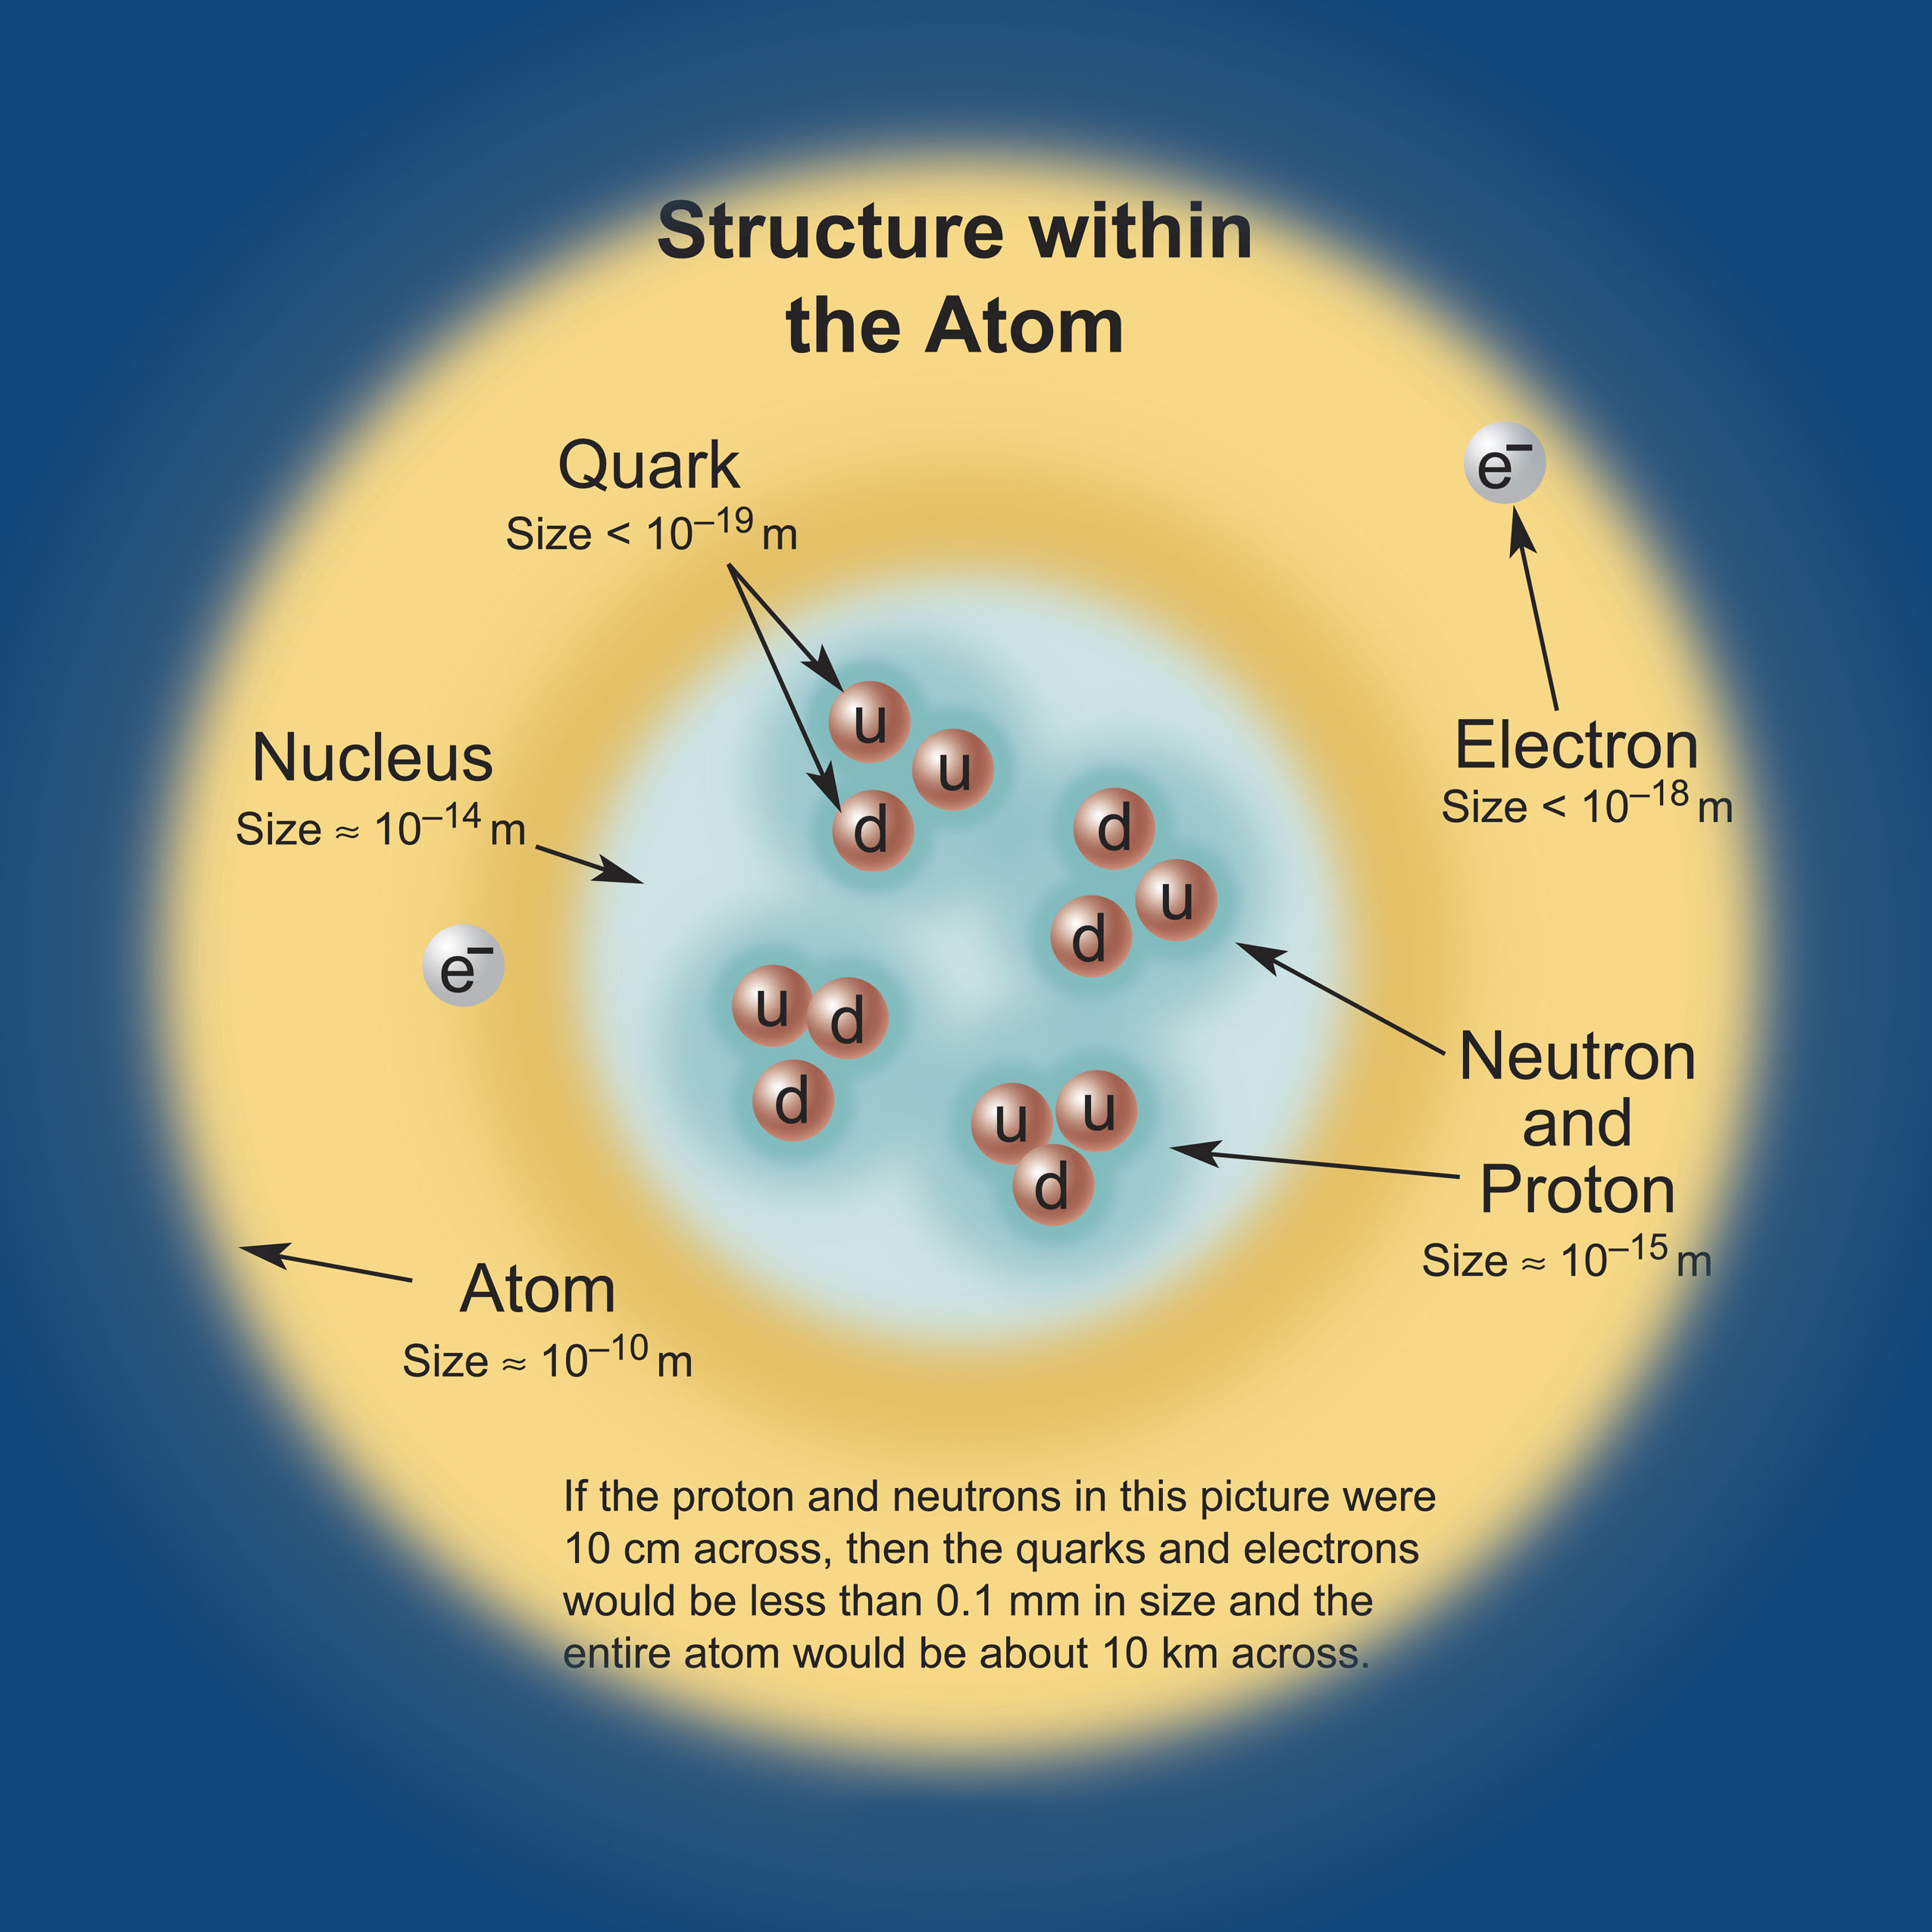
\includegraphics[width=0.70\textwidth]{atom_structure}
    \caption{The structure of an atom. Approximate scale values are indicated.}
    \label{atom_structure}
\end{figure}

Quarks were proposed by Gell-Mann and also by Zweig to explain periodicity in properties of observed subatomic particles.  \cite{griffiths_hep}. Quarks come in three families, or generations, and are arranged into doublets. Each doublet has an "up" quark with the electric charge $-1/3$ and a "down" quark with the charge $+2/3$. For antiquarks signs are reversed. The fact that the charge values were fractional was so revolutionary that Gell-Mann decided not to publish his article in a highly prestigious journal but, expecting a rejection, decided to go with the second tier one \cite{griffiths_hep}. In addition to charge, quarks also have a "flavor" number assigned to them. For instance, a charm quark has $+1$ unit of "charmness", while a strange quark has $-1$ unit of "strangeness". All the other quark flavor fields are zero for them. And this pattern is applied to all the other four quarks to fill the corresponding "quarkness" numbers. Besides, the mass of quarks increases from the first to the third family. No explanation exists in the Standard Model (SM), masses are the parameters in this theory, even though the SM is the most tested theory of fundamental forces and elementary particles, extremely successful and is presently generally accepted by the whole physics community. However, it is hypothesised that the SM could be a part of the larger ultimate theory, the so-called "The Theory of Everything" (TOE), which is to be written (had been a lifelong journey of another genius, Einstein \cite{aps_einstein}). There is hope that the TOE will be able to explain the phenomenon of the quark mass hierarchy. Another important characteristics of quarks has been revealed at the $e^+e^-$ colliders when physicists compared production rates of muons and hadrons. The theory was off by a factor of three. This was the motivation to introduce three quark colors: green, blue, and red. 


%Since it was mentioned that the atoms contain electrons, it is a good time to talk about leptons. 
Electrons that we discussed before were the first leptons to be observed in an experiment. In particle physics, a lepton is an elementary particle with the spin 1?2 that participates in all but strong interactions. All the elementary particles are split into two classes: fermions and bosons. Particles with the half-integer spin 1/2 (quarks and leptons) are called fermions since they obey Fermi-Dirac statistics ~\cite{statmech}. The other class of particles is bosons. They are force carriers, have an integer spin, and are characterised by the Bose-Einstein statistics. 

An electron (a charged lepton) was discovered by Thompson \cite{Davis:1989898} in 1897 when he was studying the properties of a cathode ray. Due to this discovery, that year is considered the beginning of an era of a particle physics: a dozen of particles has been discovered in the next decades. In 1936, another lepton was observed, a muon \cite{Piccioni1996}, in an experiment of Anderson and Neddermeyer who studied cosmic radiation. A muon is almost a copy of an electron, but is 207 times heavier. There is a story that Feynman was able to derive the mass of the muon starting with the mass of an electron, but the world has never seen that calculation published \cite{Bender}. 


Analogously to quark families, leptons are also arranged in generations. Each generation is a doublet that consists of a charged lepton (electron, muon or tau) with the charge $-1$ and a neutral lepton (corresponding electron, muon, or a tau neutrino). An electron and a muon neutrinos have been discovered in 1956 and 1962, respectively. 
The existence of the electron neutrino was deduced from the violation of the conservation of energy in a beta decay, while the muon neutrino \cite{PhysRevLett.9.36} was discovered by Schwartz, Lederman, and Steinberger during an experiment with the pion beam where leptons from the pion decays arrive to the aluminum spark chamber after passing the steel wall. 51 events of interest have been observed after running the experiment for several months.
Those events could not be due to electron neutrinos, since they will interact with the metal and produce electrons. The presence of narrow muon tracks in the chamber in each event, hence  muons, was a clear indication that those neutrinos were of a different kind, they were muon neutrinos. Finally, a tau lepton and a tau neutrino were discovered in 1975 and 2000 correspondingly \cite{PhysRevLett.35.1489, Kodama:2000mp}. With that, all three families of the SM leptons were observed: a long-awaited tau neutrino, which was decades ago theoretically speculated to exist, was finally discovered experimentally. In a like manner to families of quarks, lepton masses grow with the generation, where a tau from the third generation is the heaviest lepton. To classify leptons of different families the lepton numbers have been reserved: 1 unit of electron number to an electron and an electron neutrino, 1 unit of muon number to a muon and an muon neutrino, and 1 unit of tau number to a tau and a tau neutrino. In the SM all neutrinos are massless, however, it has been shown that they have a non-zero mass \cite{Bilenky:2014ema}. This fact is one of the main motivations for theorists to look for extensions of the SM. 

In the SM there are four fundamental forces: gravitational, weak, electromagnetic, and strong forces. 
%At the fundamental level the world is made of quarks and leptons. And there must be rules, at least we expect them to exist, which explain how quarks/leptons interact. These rules are referred to as fundamental forces of nature. 
We will classify all four forces \cite{wolfram} in terms of the relative strength, the range that they can cover, the spin of the mediator, and whether the force's nature is attractive, repulsive, or both. This should be taken with the grain of salt though, since this is quite ambiguous categorisation, but it has a deep pedagogical meaning because it helps to illustrate in which regime each of the forces is dominant. And this is one of the main approaches in solving physics problems: to know which effects are the dominant, which are sub-dominant, and which can be neglected so that correct approximations could be made and it would become possible to do calculations for problems where closed-form solutions do not exits, which is almost all the phenomena around us \cite{Bender}. 

The gravitational force governs the Universe at the macroscopic level: planets, solar systems, etc. The first theory of gravity was formulated by Newton \cite{Chandrasekhar:1187874} and then further developed by Einstein. A good historical perspective is available at \cite{Gutfreund:1980674}. It is worth noting that the gravitational force is not included in the SM. Attempts are ongoing to expand the SM, e.g., adding the graviton as a mediator, but no real success so far has been achieved to create a renormalizable theory that would combine both SM and gravity \cite{butterworth2014smashing}. To surprise of many, gravity is the weakest force, the only reason why the motion of planets and galaxies is governed by gravity is because those are gigantic objects. Gravity effects become the dominant ones at the macroscopic scale because of an enormous number of particles involved in the interaction. If the strength of the strongest force, which is the strong force, is set to 1, then the strength of the gravity will be about $10^{-41}$. It is contemplated that the gravity mediator (the graviton), if exists, would have a charge of zero, zero mass, spin 2, and should be a stable particle. The gravitational force is of the infinite range and its nature is purely attractive, while all other three forces can exhibit both an attractive and a repulsive behaviour. Einstein's general relativity theory is the only proven working theory of gravity as of now, though not a quantum theory. %, and sometimes is called "geometrodynamics". 

The next force we are going to discuss is the weak force. It is mediated by a charged W (charge +1/-1) boson or a neutral Z boson, thus giving name to charged and neutral weak interactions correspondingly. All SM fermions experience the weak force, both quarks and leptons. %For leptons, it is worth mentioning here that neutral leptons have no charge, thus will not participate in the electromagnetic interactions, and all leptons have no color charge, so they feel no strong force \cite{griffiths_hep}. 
The relative strength of the weak force is $10^{-16}$ and the range of applicability is $10^{-3}$ fm. All three weak bosons ($W^+$, $W^-$, and Z) have spin 1 and are quite massive: $m_{W^\pm} = 80. 385$ GeV and $m_{Z}=91.189$ GeV. GeV is the unit of the so-called "natural system of units", in which $\hbar = c = 1$. This system is very popular in the high-energy physics and is widely used in this thesis. Adoption of this system simplifies how many equations look and also makes a fine-structure constant $\alpha \approx 1/137$ dimensionless. Using the natural system of units \cite{Cottingham:1026625} masses, momenta, and energies are measured in electronvolts (eV), with GeV ($10^9 $~eV) and TeV ($10^{12}$~eV) being the most popular units in a modern high-energy physics due to energy regimes involved. 




For leptons charged weak interactions are interesting due to the fact that a primitive interaction vertex can be thought of as a point where a charged lepton is converted to a neutral lepton or vice versa. A good example is a muon decay, which is nothing but a conversion of the muon to a muon neutrino with the help of the W boson, which further decays to an electron and a corresponding electron antineutrino. %Lepton numbers are conserved during weak interactions and conversions happen only within the same family of leptons. However, c
It is worth noting that charged weak interactions do not conserve the flavor of quarks, e.g., members of doublets of the third and the second families can be converted into members of the lower family of quarks. This fact is reflected in the Cabibbo-Kobayashi-Maskawa (CKM) matrix \cite{pdg}, which contains information on the strength of the flavour-changing weak interactions. Since diagonal elements of this matrix are less than one and off-diagonal elements are non-zero, CKM matrix represents a mismatch of quantum states of quarks when they propagate freely and when they take part in the weak interactions. The matrix with non-zero off-diagonal elements means cross-generation interactions are allowed and this is the information that the CKM matrix quantifies.

\begin{equation}
\small
\begin{pmatrix}
|V_{ud}| & |V_{us}| & |V_{ub}| \\
|V_{cd}| & |V_{cs}| & |V_{cb}| \\
|V_{td}| & |V_{ts}| & |V_{tb}|
\end{pmatrix} = \begin{pmatrix}
0.97427 \pm 0.00015 & 0.22534 \pm 0.00065 & 0.00351^{+0.00015}_{-0.00014} \\
0.22520 \pm 0.00065 & 0.97344 \pm 0.00016 & 0.0412^{+0.0011}_{-0.0005} \\
0.00867^{+0.00029}_{-0.00031} & 0.0404^{+0.0011}_{-0.0005} & 0.999146^{+0.000021}_{-0.000046}
\end{pmatrix}.
\label{eq:ckm}
\end{equation}
Moreover, W and Z bosons can couple to each other, so $WWZ, WWWW$, and $WWZZ$ vertices are possible in the SM. Finally, since W boson participates in charged interactions, it also couples to photons, so $\gamma WW$, $\gamma WWZ$, and $WW\gamma\gamma$ vertices are also allowed.

Now, we are moving to the electromagnetic (EM) force. This is one of the main forces that we experience in our everyday life. The reason the reader can sit in the chair and do not fall further down due to gravity, is that electrons of the reader's body repel electrons of the chair. Relative strength of the EM force is $10^{-3}$ and the range of applicability is infinite. A photon, as its mediator, has zero mass, spin 1, and the theory that describes its interaction with leptons and quarks is called quantum electrodynamics (QED), developed in 1940th and 1950th by Tomonaga, Schwinger, Feynman, and Dyson \cite{qed_fathers}. Electric charge is conserved in EM interactions and no single photon-to-fermion vertex is possible, there are always two fermions that must be involved.% in such a way that their net electric charge is zero. 
Lastly, even though Z boson is massive and photon is massless, Z boson is neutral, thus, any interaction where the photon is a force carrier, can be also mediated by the Z boson.


Finally, we can talk about the forth force of the SM - the strong force. This is the strongest known force, where the gluons are the carriers. There are nine types of gluons and each gluon carries one unit of color and one unit of anticolor. But, technically, the ninth gluon is a color invariant, and would give rise to an infinite range of the strong force, which contradicts experiments. That is why modern physics assumes that in our world only eight gluons exist \cite{griffiths_hep, pdg}.

Gluons carry color charge and can couple to each other. For several high order processes in quantum chromodynamics (QCD), 3- and 4-gluon vertices have to be introduced to restore gauge invariance and no higher order vertices are required \cite{Mangano:454171}.
 
Interactions of the elementary particles that are allowed in the SM and corresponding simple vertices are shown at the Fig. \ref{SM_vertices}. 
	
\begin{figure}[H]
  \centering
    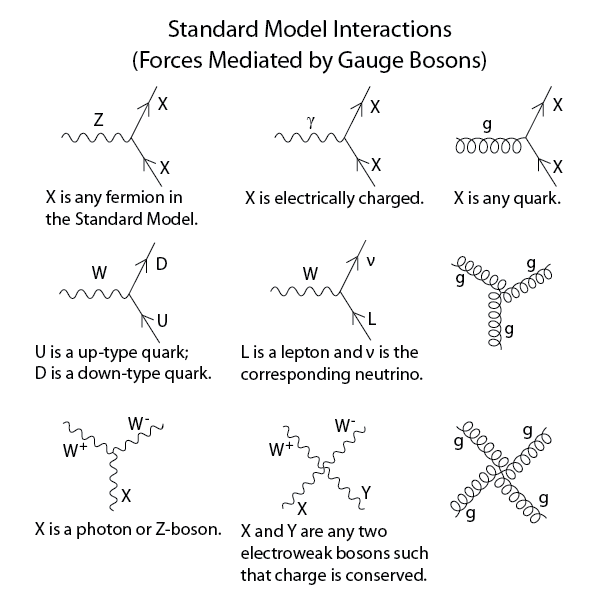
\includegraphics[width=0.80\textwidth]{Standard_Model_Feynman_Diagram_Vertices}
    \caption{All SM interaction and simple vertices. }
    \label{SM_vertices}
\end{figure}



	
The whole SM picture will not be completed without the main particle yet missing until 2012th ... the Higgs boson! (Fig. \ref{sm_interactions2} \cite{strassler}) After the electroweak (EW) unification by Glashow, Salam, and Weinberg \cite{Glashow:1961tr}, it was still not clear what is the origin of the mass of fundamental particles. In 1964, Robert Brout and Fran�ois Englert\cite{PhysRevLett.13.321}, Peter Higgs\cite{PhysRevLett.13.508}, Gerald Guralnik, C. Richard Hagen, and Tom Kibble \cite{PhysRevLett.13.585} (BEHGHK authors), proposed the method by which the particles can acquire mass. 
This technique consists of three stages and we will discuss all three of them:

\begin{figure}[H]
  \centering
    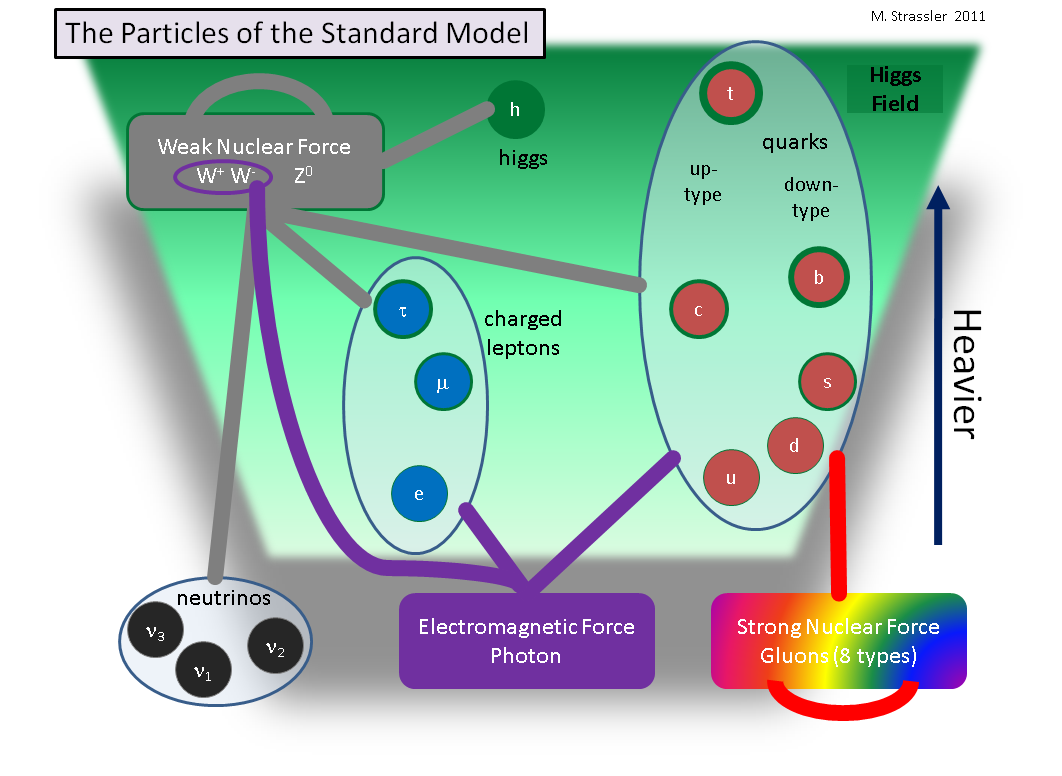
\includegraphics[width=0.80\textwidth]{sm_interactions2}
    \caption{SM particles and force carriers. Self-interactions are also shown. The strength of the coupling to the Higgs boson increases from the bottom to the top, which is illustrated by the shades of the green color (the Higgs field).  }
    \label{sm_interactions2}
\end{figure}



\begin{enumerate}
\item The Brout-Englert-Higgs (BEH) mechanism
%\begin{enumerate}
%\item Nested item 1
%\item Nested item 2
%\end{enumerate}
\item The BEH field
\item The Higgs boson.
%\ldots
\end{enumerate}

The BEH mechanism is simply a spontaneous symmetry breaking (SSB) mechanism, which is a mathematical trick consisting of rewriting the original scalar fields in the EW Lagrangian, rearranging equations, and requiring that the fields are real. What does this lead to? We started with a scalar complex field and a massless vector field and after SSB we obtained a single real scalar field (Higgs boson) and a massive vector field. In our physical world this gives mass to W and Z bosons. 

The BEH field exists everywhere and has been present almost since the Big Bang \cite{who_cares}. It is a property of our world. All the fundamental particles that interact with the BEH field acquire mass. Those, who do not interact directly (at the tree level), have no mass and all their energy is in the form of the momentum, thus they can travel with the speed of light. The more the particle interacts with the BEH field, the higher is the coupling to the Higgs boson or simply the higher is the mass of the particle. For example, the coupling of the Higgs boson to fermions is proportional to the mass of the fermions, while for W and Z bosons it is proportional to the squared mass of bosons, thus top quark and Z bosons are quite massive (see Fig. \ref{coupling_ff} \cite{CMS-PAS-HIG-14-009}). 

\begin{figure}[H]
  \centering
    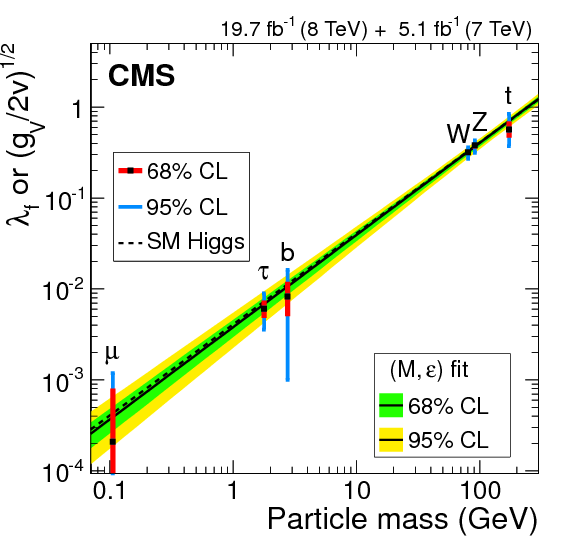
\includegraphics[width=0.80\textwidth]{coupling_ff}
    \caption{Coupling of particles to SM Higgs boson versus the mass of the particle, log-log scale is used.}
    \label{coupling_ff}
\end{figure}



Now let us talk about the Higgs boson. First a little bit of history, an irony of life, actually. The BEH particle is called the Higgs boson, but Peter Higgs was not the first to publish the article on the BEH mechanism, in fact he was the last out of BEHGHK authors! His very first article was rejected since it contained no specific predictions or conclusions drawn from his calculations. This is why he was out-published by others. But this rejection made him write another article where he explicitly predicted an existence of the new boson. And this is what has made all the difference, he was the first to predict a new boson, and this boson now is called the Higgs boson. The Higgs boson is the excitation of the BEH field. Thus, the Higgs bosons can be produced at colliders by pumping more and more energy in a small space-time region exciting the BEH field to "produce" the Higgs bosons. In reality this happens through making the LHC beams more energetic and thus, during the collision, having more energetic gluons (and also quarks). The main production mechanism is called a gluon fusion, when through the top quark loop a single Higgs boson is produced. This accounts for about $90\%$ of the overall LHC Higgs production at the 13 TeV energy. The second mechanism is a vector boson fusion. The third mechanism is the associated production with a weak boson. And the smallest contributor to the Higgs boson production is the ttH process, which stands for the associated production of the Higgs boson with the top anti-top quark pair.% (see Fig. \ref{higgs_production}). 
All mentioned Higgs boson production mechanisms are presented in the form of Feynman diagrams in Fig. \ref{higgs_production}.

\begin{figure}[H]
  \centering
    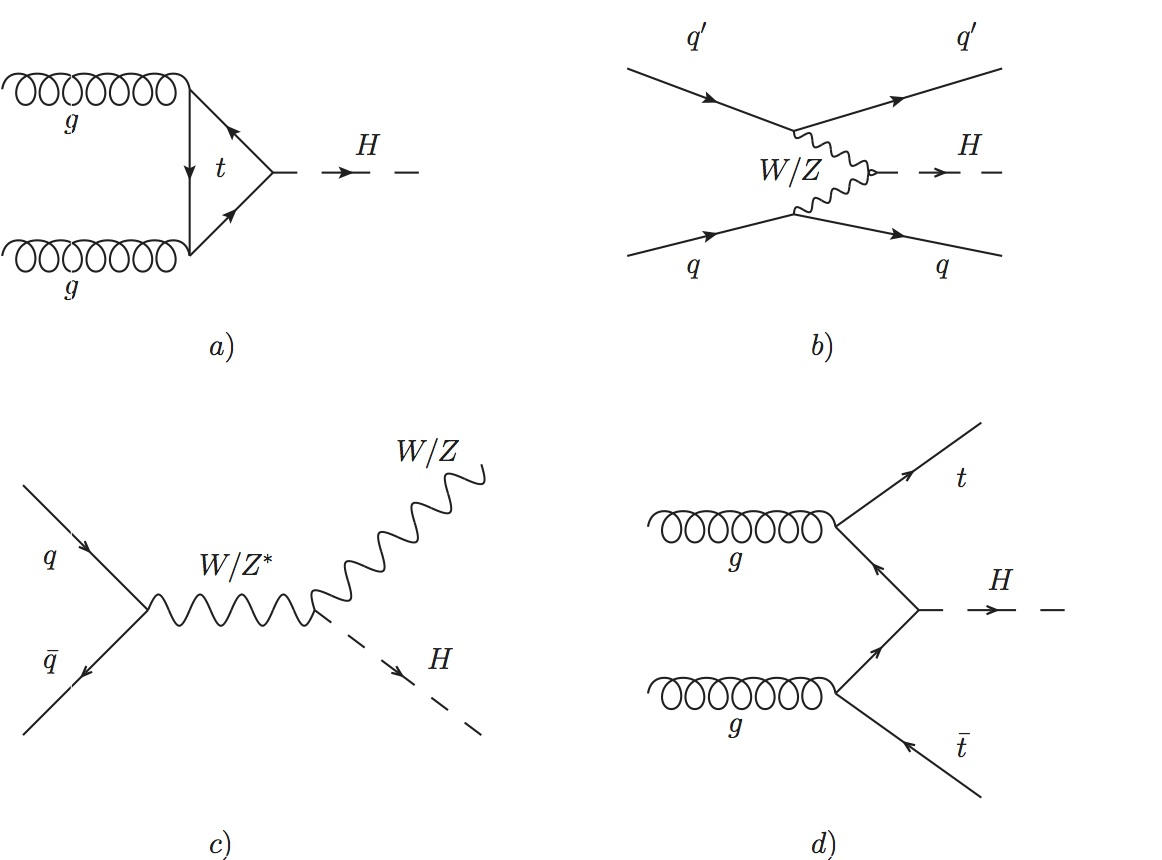
\includegraphics[width=0.90\textwidth]{higgs_production}
    \caption{SM Higgs boson production modes: a) a gluon fashion, b) a vector boson scattering,  c) an associated production with a vector boson, d) an associated production with the top anti-top pair. }
    \label{higgs_production}
\end{figure}


The final important aspect of the Higgs boson physics is the decay channels of the Higgs boson, in other words probabilities with which Higgs boson decays to other particles, so called branching fractions (see Fig. \ref{Higgs_BR_LM_RECT}). This analysis focuses on two Higgs boson decays, $H\to b\bar{b}$ and $H\to ZZ$. The first one has the highest branching ratio, while the second one gives a clean signature when subsequent $Z \to \ell\ell$ decays are selected. 




\begin{figure}[h]
  \centering
    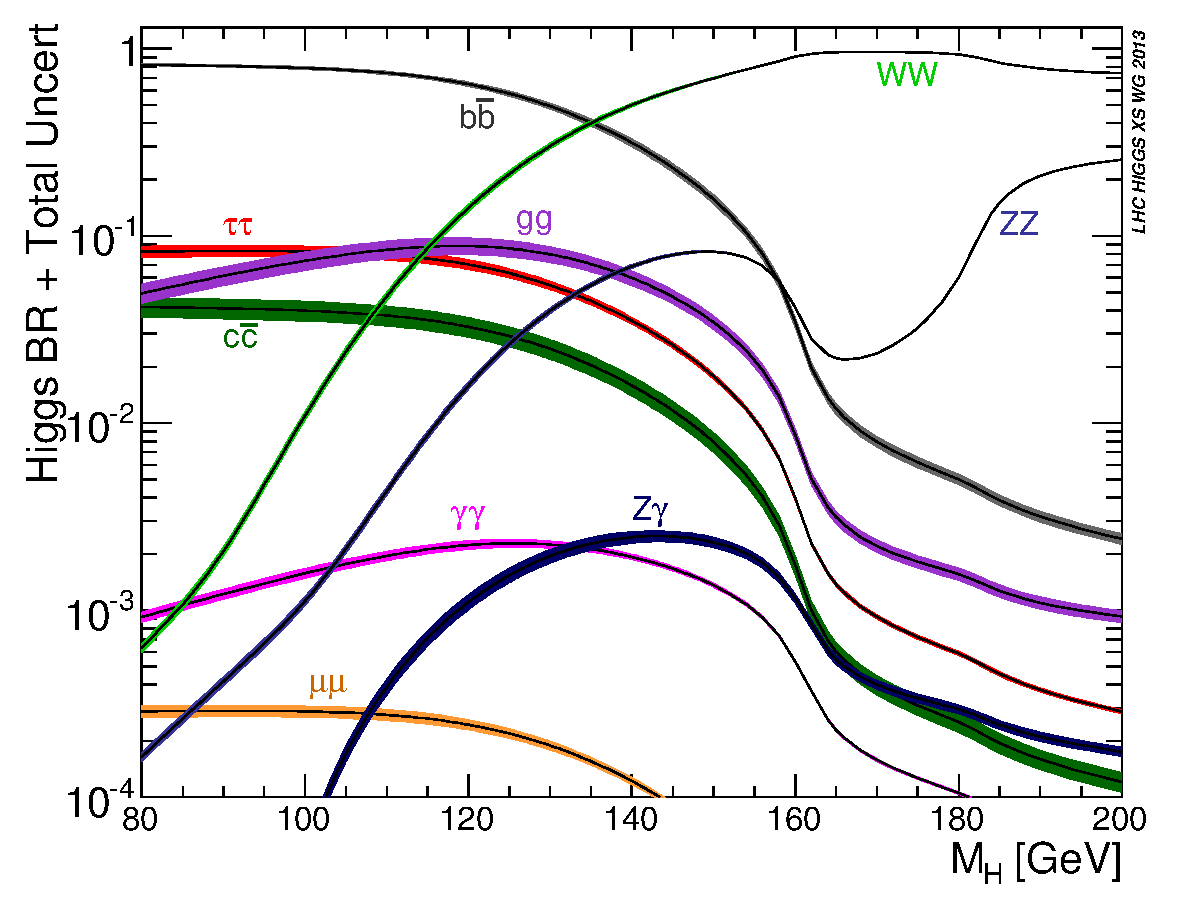
\includegraphics[width=0.90\textwidth]{Higgs_BR_LM_RECT}
    \caption{Higgs boson decay channels. At 125 GeV the dominant decay mode is $H \to b\bar{b}$.}
    \label{Higgs_BR_LM_RECT}
\end{figure}







%\hyphenation{se-para-tion}
\hyphenation{theo-re-ti-cal}
\hyphenation{handed-ness}
\hyphenation{fo-llo-wing}
\hyphenation{ac-cor-ding}

\chapter{Theory}
\label{ch:theory}


In the previous chapter, we introduced the SM and discussed the particles and their interactions that are described by this theory. In this chapter we will start with the general mathematical formalism of the SM. Then, in the second part we will focus on the double Higgs boson physics described in Beyond the Standard Model (BSM) theories.

\section{Lagrangian formalism of the Standard Model}


\indent The SM uses Lagrangian mechanics as the mathematical approach to describe quantitatively the interactions of elementary particles and fields. 
The SM Lagrangian can be split into four main contributions \cite{Mozer:2016wzi}:
\begin{equation}\label{lagr_SM}
\Lagr_{SM} = \Lagr_{Yang-Mills} + \Lagr_{ferm} + \Lagr_{H} + \Lagr_{Yuk} 
\end{equation}

\noindent where

\begin{itemize}
\item $\Lagr_{Yang-Mills}$ represents gauge bosons and their \textcolor{black}{self-}interactions,
\item $\Lagr_{ferm}$ describes fermions and their interactions with the gauge bosons, 
\item $\Lagr_{H}$ characterises the Higgs boson, its self-interaction, and its interaction with the gauge bosons to give them mass, 
\item $\Lagr_{Yuk} $ gives details of fermions and their interactions with the Higgs boson, which, through the Yukawa mechanism, give mass to fermions.
\end{itemize}
 

The first term in the SM Lagrangian in full can be written as:
\beqn\label{lagr_Yang-Mills}
\Lagr_{Yang-Mills} = 	-\frac{1}{4}W^i_{\mu\nu}(x)W_i^{\mu\nu}(x) -\frac{1}{4}B_{\mu\nu}(x)B^{\mu\nu}(x) -\frac{1}{4}G^a_{\mu\nu}(x)G_a^{\mu\nu}(x)
\eeqn

\noindent where

\begin{align}
B_{\mu\nu}(x)   \equiv & \partial_\mu B_\nu -  \partial_\nu B_\mu \label{B_tensor} \\ 
W^i_{\mu\nu}(x) \equiv & \partial_\mu W^i_\nu(x) - \partial_\nu W^i_\mu(x) - g \varepsilon^{ijk}W^j_\mu W^k_\nu \label{W_tensor}\\
G^a_{\mu\nu}(x) \equiv & \partial_\mu G^a_\nu(x) - \partial_\nu G^a_\mu(x) - g_s f^{abc}G^b_\mu G^c_\nu \label{G_tensor}
\end{align}


\noindent with $\mu$ and $\nu$ indices running from 0 to 3, \textit{SU(2)} indexes $i,j,k = 1,2,3$, and \textit{SU(3)} indices given by $a,b,c = 1, ..., 8$. Terms $\partial_\mu$ and $\partial_\nu$ represent four-vector covariant derivatives. According to the Noether's theorem, each symmetry is intrinsically connected to a conservation law \cite{Sardanashvily:2143630}. The invariance of the Lagrangian under certain transformations or, in other words, how the fields in the Lagrangian ($\Lagr_{Yang-Mills} $ in this case) are related to their corresponding underlying symmetries, is explained in the following way: 

\begin{itemize}
\item $B_{\mu\nu}$ corresponds to \textit{$U(1)_Y$} symmetry of the weak hypercharge $Y_k$ with \textit{U(1)} being a unitary one-by-one matrix (a scalar), 
\item $W^i_{\mu\nu}$ corresponds to \textit{$SU(2)_I$} symmetry of the weak isospin $I^i_{w}$. Another common representation is \textit{$SU(2)_L$}, since only left-handed SM fermions are transformed under this symmetry. \textit{$SU(2)_L$} is a unitary two-by-two matrix with the determinant equal to one. 
\item $G^a_{\mu\nu}$ corresponds to \textit{$SU(3)_c$} symmetry of the QCD color charge with \textit{$SU(3)_c$} being a unitary three-by-three matrix with the determinant equal to one.
\end{itemize}

\noindent The "B" field is a kinematic term, "W" and "G" terms describe interactions among the gauge bosons, $g$ and $\varepsilon$ are \textit{$SU(2)_L$} coupling and structure constants, $g_s$ and $f$ are coupling and structure constants for \textit{$SU(3)_c$}.


The second term in the SM Lagrangian is: 
\beqn\label{lagr_ferm}
\Lagr_{ferm}= i \bar{\Psi}_L \slashed{D} \Psi_L  + i \bar{\psi}_{l_{R}}  \slashed{D} \psi_{l_{R}} +
i \bar{\Psi}_Q \slashed{D} \Psi_Q  + i \bar{\psi}_{u_{R}}  \slashed{D} \psi_{u_{R}} +
 i \bar{\psi}_{d_{R}}  \slashed{D} \psi_{d_{R}}
\eeqn

\noindent Notice, that the mass terms are still absent. In Eq. \ref{lagr_ferm}, $\Psi$ represents a doublet of a charged lepton and a corresponding neutral lepton within the same lepton family of \textit{$SU(2)_L$}. The subindex Q is reserved for a family of quarks, and $\psi_R$ describes a right-handed leptonic singlet.  Gauge boson interactions are present due to the derivative term:
\begin{align}\label{cov_der2}
D_\mu = \partial_\mu + ig I_w^i W_\mu^i+ ig' Y_w B_\mu + ig_s T_c^a G_\mu^a
\end{align}

\noindent Physical fields in this notation are represented by a linear combination of W and B fields:
\begin{align}\label{neutral_fields}
A_\mu = &  B_\mu \cos\theta_W + W^3_\mu \sin\theta_W \\ 
Z_\mu = & -B_\mu \sin\theta_W + W^3_\mu \cos\theta_W \nonumber 
\end{align}
\noindent where $\theta_W$ is known as the \ti{Weinberg angle} \cite{Weinberg:799984}.

With the first two terms of the SM Lagrangian --  $\Lagr_{Yang-Mills}$ and $\Lagr_{ferm}$ -- one obtains a valid theory of fermions and bosons; however, these particles are massless in this theory \cite{Wolf:2015kua}, which evidently contradicts reality. However, one cannot simply add mass terms by hand since that would break the Lagrangian gauge invariance. To solve this issue and to ensure that weak bosons are massive, one has to follow a more complex procedure: introduce a Higgs field and an SSB procedure (see section \ref{sec:BEH}). During the SSB procedure, the $SU(2)_L \times U(1)_Y$ symmetry needs to be broken to have massive SM particles. The Higgs mechanism enters the SM Lagrangian through the corresponding Higgs Lagrangian term given by 
\beqn\label{lagr_higgs}
\Lagr_H=(D_\mu\Phi)^\dagger(D^\mu\Phi) - V(\Phi) , \qquad V(\Phi)= - \mu^2(\Phi^\dagger\Phi) + \frac{\lambda}{4}(\Phi^\dagger\Phi)^2
\eeqn

\noindent where

\beqn\label{vev}
\Phi = \binom{\phi^+}{\phi^0 = (v+H + i\chi)/ \sqrt{2}} \quad \text{with} \quad v = 2 \sqrt{\frac{\mu^2}{\lambda}}
\eeqn

\noindent and $\mu$ and $\lambda$ are parameters of the Higgs potential. The Higgs field vacuum expectation value ($vev$) $v$, after the SSB, can be expressed in terms of $\mu$ and $\lambda$. The Higgs potential before and after the SSB is shown in Fig. \ref{hp2d}. The importance of the $\Lagr_H$ in the SM Lagrangian is crucial: after rearranging terms (full derivation is available at \cite{Halzen:100339, Zee_qft}), the bosons finally have masses given by:

\beqn\label{boson_masses}
M_W = \frac{gv}{2}, \quad  M_Z = \frac{M_W}{\cos{\theta_W}}, \quad M_H = \sqrt{2\mu^2}
\eeqn



 
The final contribution to the SM Lagrangian is the Yukawa term, with Yukawa Lagrangian given by:
\beqn\label{lagr_Yuk}
\Lagr_{Yuk}=  - i \bar{\Psi}_{L}  G_l  \psi_{l_{R}} \Phi
- i \bar{\Psi}_{Q}  G_u  \psi_{u_{R}} \tilde{\Phi}
- i \bar{\Psi}_{Q}  G_d \psi_{d_{R}} \Phi + h.c.
\eeqn

\noindent where $\tilde{\Phi} = i \sigma^2 \Phi^*$. The $3 \times 3$ matrices G contain fermion masses, which are free parameters in the SM and have to be determined experimentally. These matrices  describe  the  so-called Yukawa $y_f$ couplings between the single Higgs doublet $\varphi$ and the fermions. In the case of leptons, matrices G can be diagonalised to provide mass eigenstates of definite generation. Using the mass eigenstates, the strength of the coupling of a fermion $y_f$ to a Higgs boson is given by $y_f = m_f /\textit{vev}$, where $m_f$ is the mass of a fermion and \textit{vev} is set by $\mu$ and $\lambda$ parameters, see Eq. \ref{vev}. On contrast, W and Z boson masses are predicted by the SM and are directly related to the weak couplings and the Higgs field parameters, see Eq. \ref{boson_masses}. 
%The mass of each fermion is proportional to the Yukawa coupling ($y_f$ or $\lambda_f$) of the corresponding fermion to the Higgs boson, as shown in Fig. \ref{coupling_ff}.


The Higgs boson mass is proportional to the $\mu$ parameter. In 2012, using precise single Higgs boson mass measurements from both ATLAS and CMS experiments, the value of $\mu$ was determined. Additionally, many physics analyses at CERN have been targeting the measurement of the $\lambda$ parameter, because it is related to the shape of Higgs potential. The simplest potential characterized by $\mu$ and $\lambda$ parameters, sufficient to obtain the SSB phenomenon and give mass to the SM particles, is the so-called "Mexican hat" Higgs potential. This name reflects the fact that the shape of the potential after SSB resembles the Mexican hat, see Fig. \ref{hp2d}. However, the real shape of the Higgs potential may be more complex or different from the Mexican Hat, thus, direct precise determination of the $\mu$ and $\lambda$ parameters is a sensitive tool to test the limitations of the SM and may open doors to the BSM effects. The simplest interaction suitable for probing the higher order terms of the Higgs potential directly is the one where two Higgs bosons (HH) are present. All this makes HH physics, the topic of this thesis, one of the main goals for the future High Luminosity LHC (HL-LHC) that will start operations in 2026. 

\begin{figure}[H]
\centering
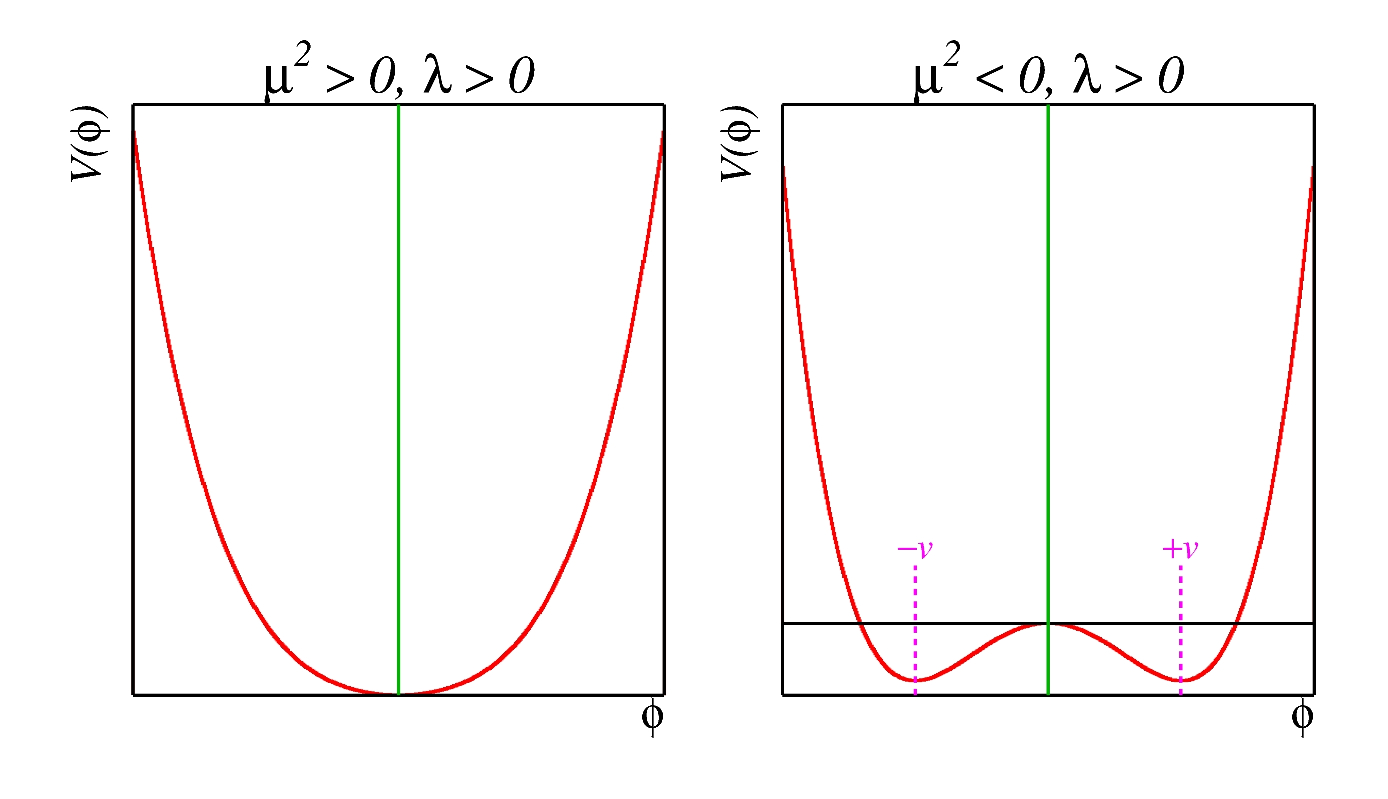
\includegraphics[width=0.7\textwidth]{hp2d}\\
\hspace{1cm} 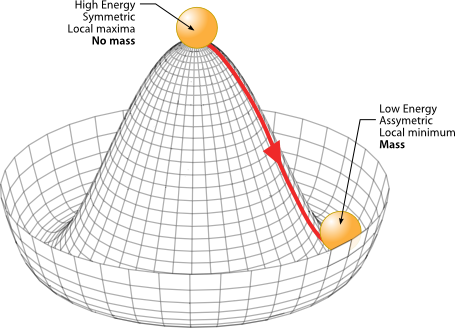
\includegraphics[width=0.44\textwidth]{higgs-hat}
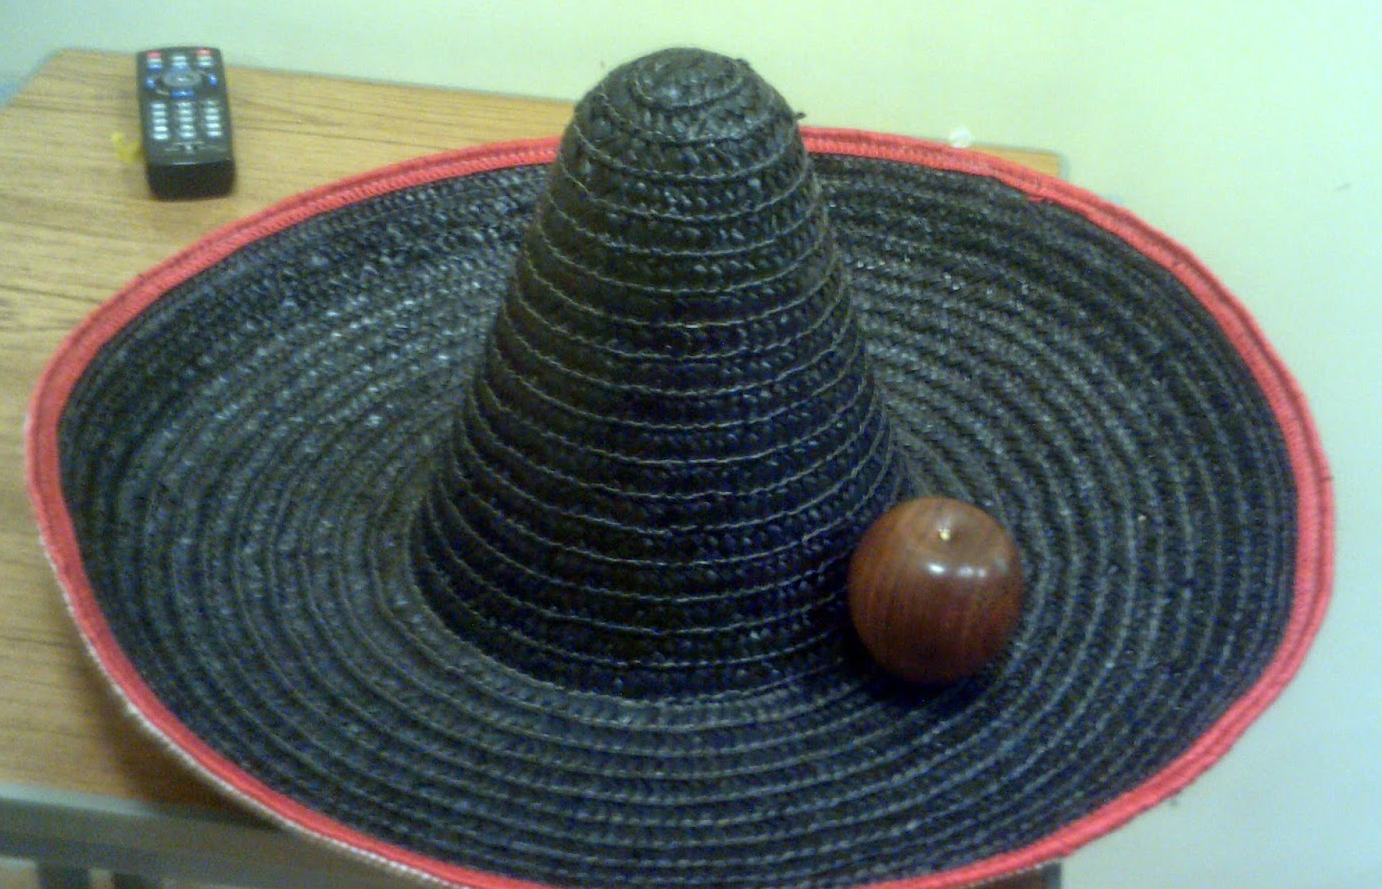
\includegraphics[width=0.4\textwidth]{mexican2}\\
\caption[SSB Potential form]{Top: Shape of the Higgs potential before and after the SSB that is determined at the leading orders by $\mu$ and $\lambda$ parameters \cite{MonroyMontanez:2639240}. Bottom Left: Schematic drawing of the Higgs potential (after the SSB) that resembles a Mexican hat. Bottom Right: A real Mexican hat.}
\label{hp2d}
\end{figure}


\section{Double Higgs in Beyond the Standard Model Theories}

%\textcolor{red}{IN THE INTRO??}
While the mass parameter $\mu$ has been measured fairly accurately, $\lambda$ parameter requires even HL-LHC to run for many years to get enough statistics since HH processes are rare and are of almost three orders of magnitude lower rate than the single Higgs boson production. Technically, the amount of the HL-LHC data is not enough to reach the sensitivity of the SM for HH processes. However, several BSM models predict resonant HH production to which the current LHC data could be sensitive. In these theories, HH is produced through a decay of a heavy resonance, which is not a part of the SM; thus, if such processes are found, a new chapter in HEP will be opened. In this thesis we focus on the resonant production of the HH system, which further decays to leptons and quarks. With the available CMS data, resonant HH analyses are starting to approach the needed sensitivity to many BSM models. 

BSM theories such as \cite{Huang:2017nnw, Dolan:2012ac, Kanemura:2016tan, Sirunyan:2018iwt, Randall:1999ee, Oliveira:2014kla} predict a resonant production of double Higgs boson events through a heavy resonance of a narrow width ($\sim O(1-10)$ GeV) \cite{Sirunyan:2018iwt}. Since the width parameter is proportional to the mass of the particle and its coupling to the Higgs boson, the values of the width larger than the $1-10$ GeV  range would correspond to BSM particles too heavy to be produced at the LHC. Additionally, from the perspective of the experimental physicist, the ``bump hunt'' of a narrow width particle is the well-established technique that led to discoveries of many particles. 


In this dissertation data is compared to predictions from the Warped Extra Dimensions theory (WED) \cite{Oliveira:2014kla}. WED theory addresses the hierarchy problem by adding an additional fifth dimension to the conception of 4-dimensional (4D) space-time. In the framework introduced by Randall and Sundrum (RS) \cite{Randall:1999ee}, 4D space is an Effective Field Theory (EFT) approximation of the higher dimensional space. The extra dimension exists between the gravity (Planck) and weak (TeV) flat 4D branes (see Fig. \ref{branes}) and is called the "bulk". In the bulk, the strength of the gravitational interaction is not uniform. It depends on the coordinate in the 5th dimension and is characterised by the exponentially decaying function.




\begin{figure}[H]
\centering
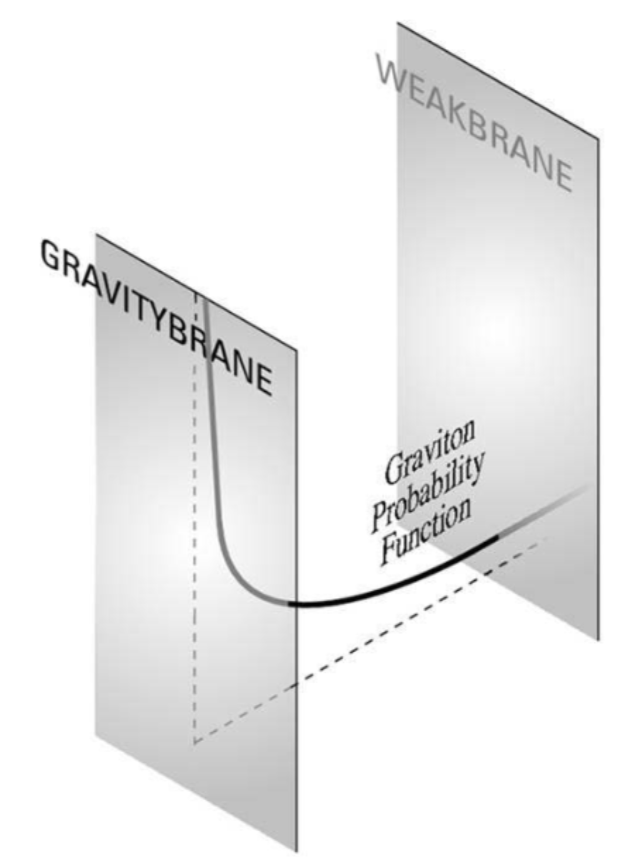
\includegraphics[width=0.4\textwidth]{branes.png}
\caption[RS branes]{5D space in the RS model \cite{Xanda}.}
\label{branes}
\end{figure}




The free parameters of the RS model are the brane separation factor $k$ and the size of the compactified dimension $r_c$. Another name for the brane separation factor is the curvature factor. This factor is given by $k \approx \sqrt{ \frac{\Lambda}{M^2_5}  }$, where $\Lambda$ is the ultraviolet cutoff of the theory and $M_5$ is the 5D Planck mass. %The radius of the extra dimension $r_c$ is proportional to the parameter $1/k$ and the logarithm of $1/vev$. 
The mass hierarchy of the SM particles between the Planck scale and the electroweak scale can be reproduced when free parameters $k$ and $r_c$ satisfy $k \cdot r_c \approx 11$. In this case, the RS model matches the observations: the Higgs boson being closer (in the geometric sense in the fifth dimenstion) to the TeV brane and light fermions being located near the Planck brane, see Fig. \ref{branes}.

In the RS model under study, two new particles appear: a graviton and a radion. When the bulk is compactified, the WED theory predicts the existence of the Kaluza-Klein (KK) \cite{Uzawa:1999pg} excitations of the gravitational field, with the zero-th KK mode being a graviton, the mediator of the gravitational force. The graviton (spin 2) is the first WED particle predicted by the RS model. The graviton can propagate freely in the full higher-dimensional space of the 5D bulk. The other RS particle is a radion (spin 0). Its existence is required to stabilise the size of the extra dimension. The WED space necessarily behaves in a quantum way, and, therefore, its size or length is subject to quantum fluctuations. The fluctuations of the length are parametrised by the radion, which is very similar to how the fluctuations of the EM field are parametrized by the photon. Goldberger and Wise \cite{Goldberger:1999uk} wrote down a potential for the radion and showed how \textit{vev} of the radion sets the length of the extra dimension to its desired value. This is the mechanism for stabilizing the WED length. Without this procedure the radion would be massless and would mediate an infinite-range interaction, which is in conflict with cosmological observations. 


Since LHC had provided us with no evidence of the SM particles interacting with the RS particles, the RS model considered in this thesis hypothesizes that SM particles are confined to branes. Another explanation of the lack of evidence of the RS particles at the LHC could be due to the fact that RS particles are too massive to be produced at the current LHC energies, but this argument is not addressed in this dissertation. 


The theoretical arguments put forward by the authors \cite{Davoudiasl:1999jd} suggest the RS parameters $k$ and $\bar{M}_{Pl}$ to be constrained by the following range of values: $0.01 \leq k / \bar{M}_{Pl} \leq 1$, where the parameter $k$ is of the order of the Planck scale and $\bar{M}_{Pl} = \sqrt{\frac{M^3_5}{k} \cdot (1 - e^{-2\pi k r_c} ) }$ is a reduced 4D $M_{Pl}$. Considered in this measurement, the graviton and radion are RS particles with a KK state mass of the order of TeV \cite{Oliveira:2014kla}. 

With a part of the KK 5D wave function, often called a profile, expressed as $f^{(n)}_X(\phi)$, where n refers to the n$^{th}$ KK mode, the graviton can be decomposed as $\sum_{n=0}^{\infty} h^{(n)}_{\mu\nu}(x_\mu) \cdot f^{(n)}_X(\phi)$. Its zero-th mode corresponds to the massless graviton and the first mode corresponds to the lightest KK graviton (later graviton) which has the mass of the O(TeV). The profiles for all the matter fields are described by a combination of Bessel and exponential functions \cite{Traczyk:2002jh, Goldberger:1999wh,Raychaudhuri:2126967}. The Lagrangian describing the interaction of the graviton with the SM fields is given then by 

\beqn\label{lagr_graviton}
\Lagr_{graviton}=  - \frac{x_1\tilde{k}}{m_G} h^{\mu\nu(1)} \times d_i T^{(i)}_{\mu\nu},  
\eeqn
where $x_1$ = 3.83 is the first zero of the Bessel function for a given profile, $\tilde{k}  = k / \bar{M}_{Pl}$, $h^{\mu\nu}$ is a tensor describing the first KK graviton field, $m_G$ is the mass of the graviton of the order of TeV, $d_i$ is an integral of the profiles of the SM fields and KK graviton, and  $T^{(i)}_{\mu\nu}$ is a 4D canonical energy-momentum tensor \cite{Forger:2003ut} for any SM field $i$. A free parameter $\tilde{k}$ varies from 0.01 to 1 when $m_{G}$ is varied from 100 to 1500 GeV. 

For the radion, the Lagrandian is given by:
\beqn\label{lagr_radion}
\Lagr_{radion}=  - \frac{r}{\Lambda_R} \times a_i T^{\mu (i)}_{\mu},  
\eeqn
where $r$ is a 5D radion field, $\Lambda_R$ is the scale parameter proportional to $k \cdot \sqrt{ ( \frac{M_5}{k} )^3}$, and $a_i$ is the coupling of the radion to the SM field $i$. In the studied RS model the profiles of the graviton and radion arise naturally as being localised at the TeV brane for the coupling of a radion and a graviton to the massive SM fields to have the value of the order of one \cite{WED}. 


In the SM, HH production is dominated by two processes, which are shown using Feynman diagram representation in Fig.\ref{SM_HH}: the "box" and the "triangle" diagrams. They interfere destructively and the total cross section is thus lowered. The total cross section made of box and triangle contributions is denoted as the ``SM'' and is shown in black color in Fig. \ref{hh_comparison} on the right. Additionally, this figure includes a BSM contribution - a non-linear (``nl'') term $t\bar{t}HH$ that vanishes in SM, but may be present in BSM \cite{Contino:2012xk}. The results shown in Fig. \ref{hh_comparison} right, have been produced by theorists \cite{Chen:2014xra} for 100 TeV collider. However, the distributions of the double Higgs mass as well as amplitudes remain to a high degree unchanged between 13-14 and 100 TeV (see Fig. \ref{hh_comparison} on the left) - therefore, one assumes that amplitudes would look similarly for 13 TeV. 

\begin{figure}[H]
  \centering
    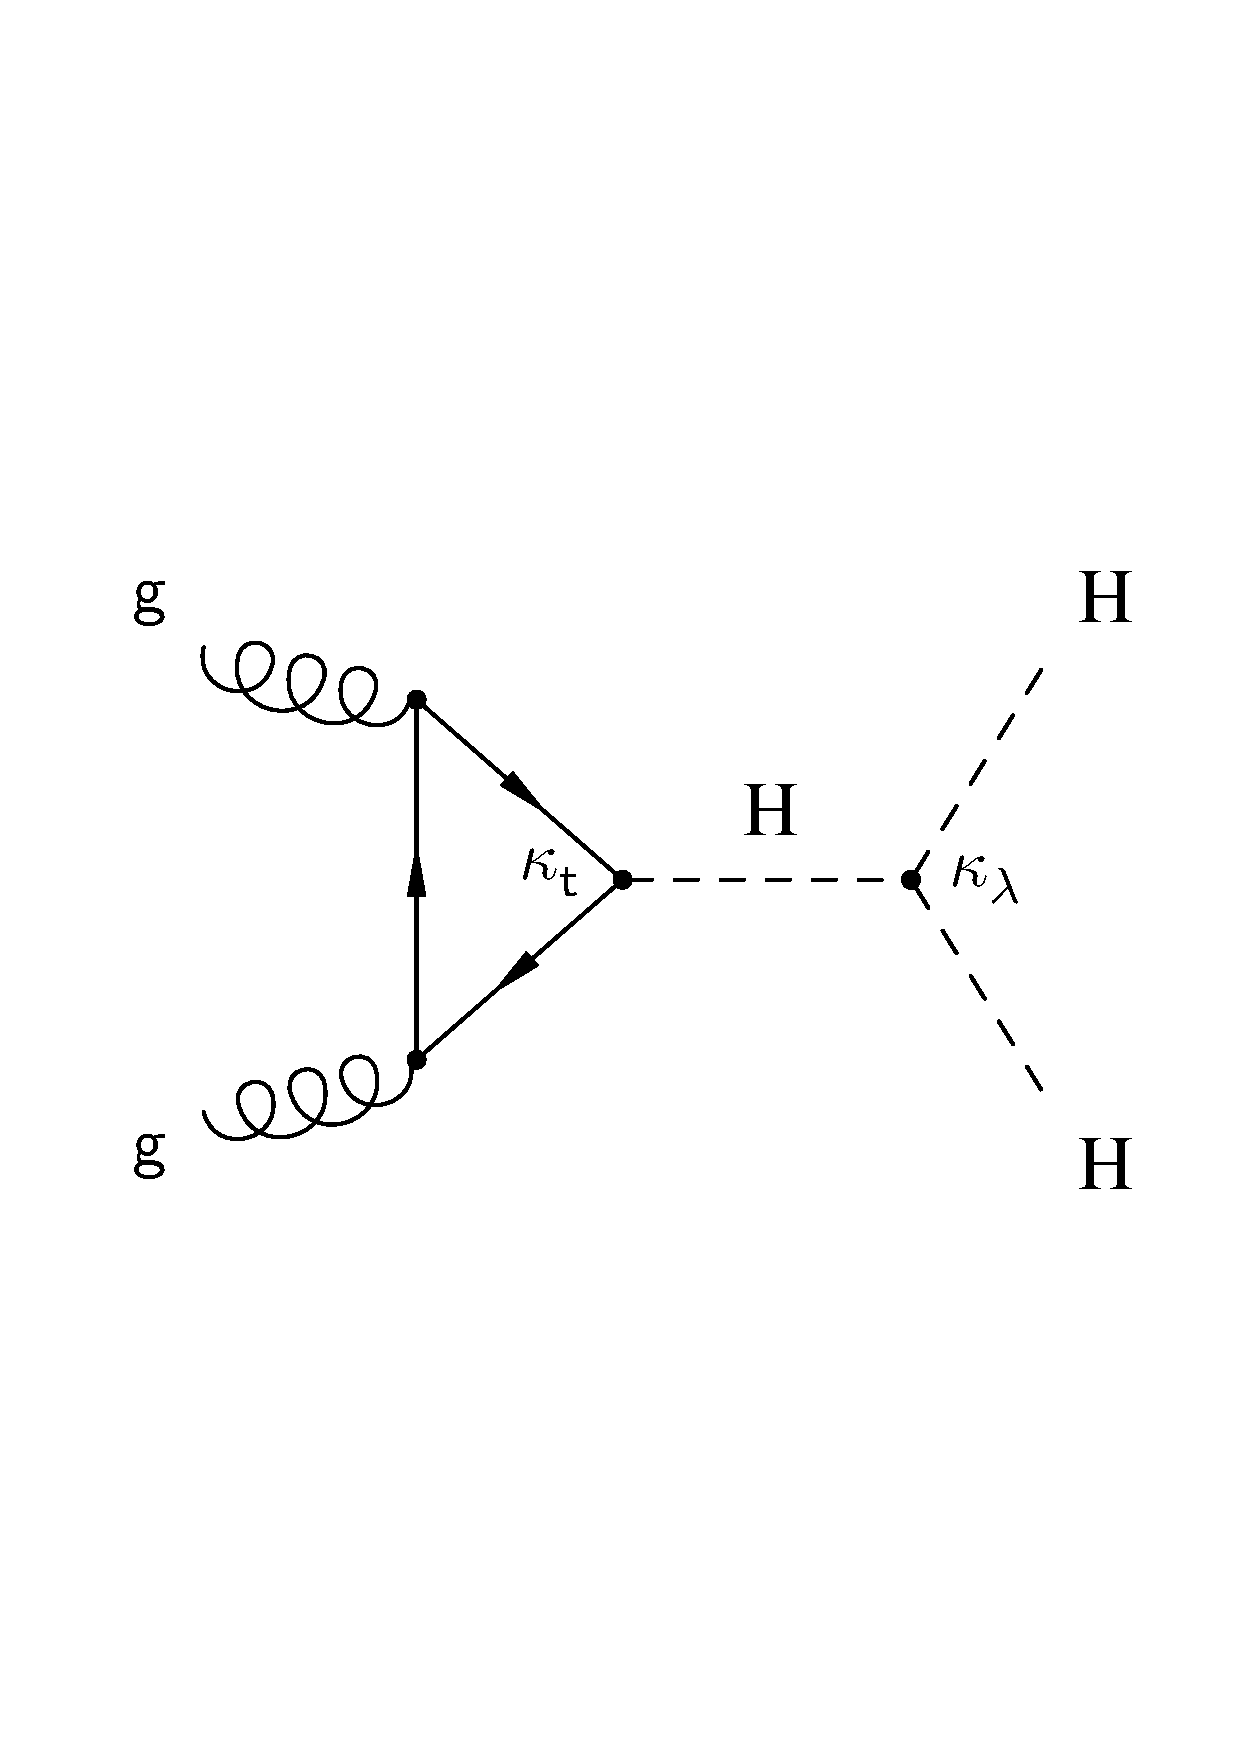
\includegraphics[width=0.49\textwidth]{hh_tri}
     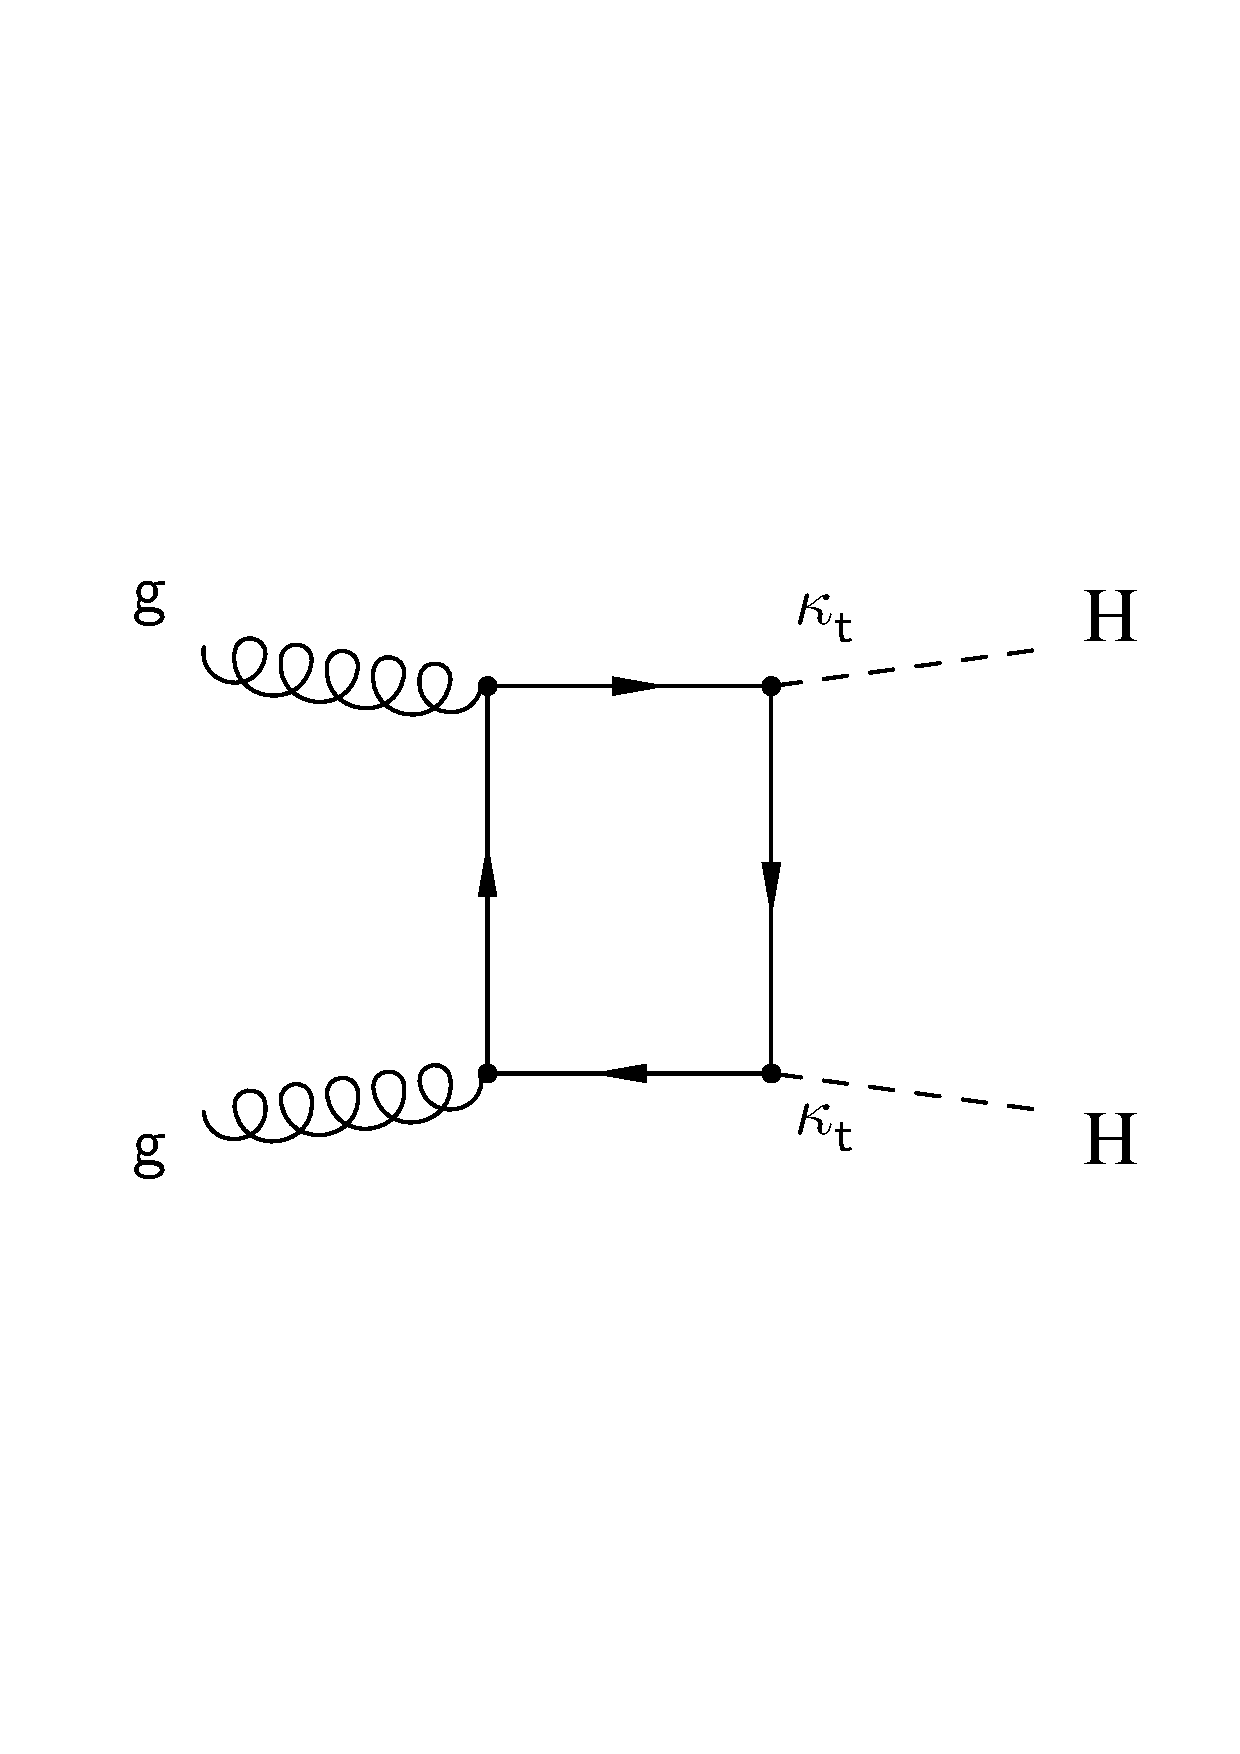
\includegraphics[width=0.44\textwidth]{hh_box_2}
    \caption[SM double Higgs boson production]{SM double Higgs boson production. Left: the triangle diagram with the virtual top quark loop. Right: the box diagram which dominates the overall HH production rate.}
    \label{SM_HH}
\end{figure}

The box diagram dominates the double Higgs boson production and peaks near 400 GeV of the di-Higgs mass \cite{Chen:2014xra}. Even though the Fig. \ref{hh_comparison} on the right illustrates the SM double Higgs production, which is a non-resonant process, the amplitudes are not flat. Two factors contribute: an amplitude decreases with the COM and, at the same time, the kinematic turn on of the production of the di-Higgs system is always present. 



\begin{figure}[H]
  \centering 
    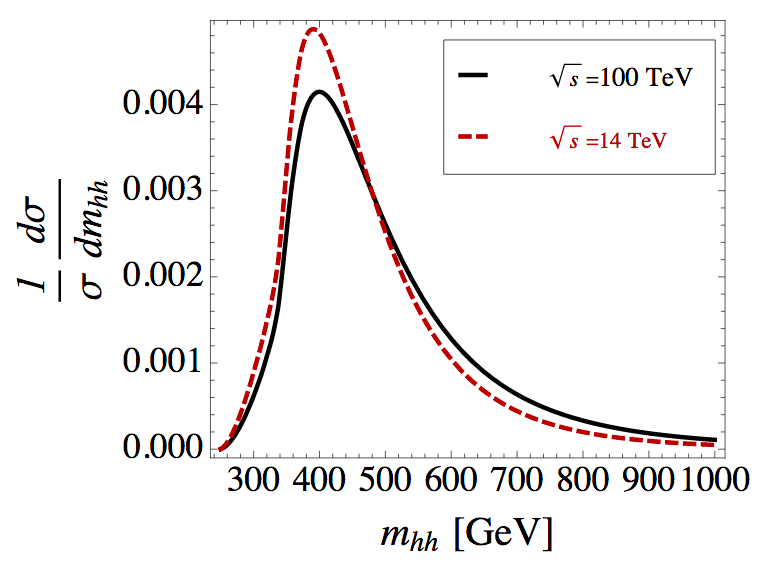
\includegraphics[width=0.49\textwidth]{hh_14_100_comparison}
    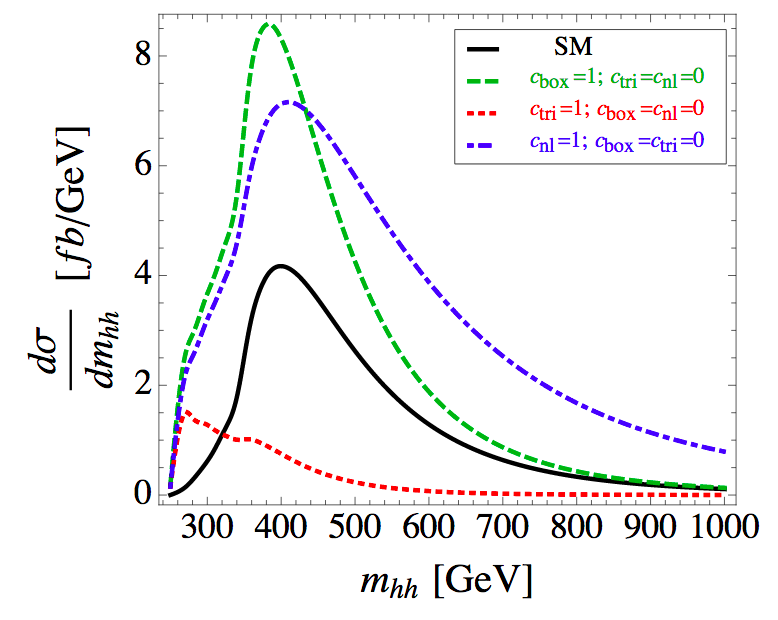
\includegraphics[width=0.49\textwidth]{hh_sm_comparison}
    \caption[Double Higgs mass distribution and the total cross-section]{Left: comparison of the double Higgs boson mass distribution in the SM at the LO at 14 and 100 TeV center-of-mass energy. Right: the total SM HH cross section and the individual contributions \cite{Contino:2012xk}. Green refers to the SM box production, red refers to the SM triangle production, and blue refers to BSM non-linear $t\bar{t}HH$ production, not included in the total SM production in black \cite{Chen:2014xra}. }
    \label{hh_comparison}
\end{figure}




In this measurement, the gravitons and radions in the search are expected to be produced by a BSM "contact interaction" Feynman diagram allowed by the WED scenario. This process is shown in Fig. \ref{HH_signature}.  A graviton and a radion decays to a pair of Higgs bosons are thoroughly studied theoretically \cite{Chen:2014xra, HHXsec, Contino:2012xk}. Experimental results produced by this measurement are compared to the theoretical predictions calculated for the WED model with the standard benchmark parameters $\tilde{k}=0.1$ and $\Lambda_R = 3 $ TeV \cite{Wertz:2632195, Cadamuro:2292733}. These reproduce SM observations and allow the production of the RS particles that can be observed at the LHC. 





\begin{figure}[H]
  \centering
    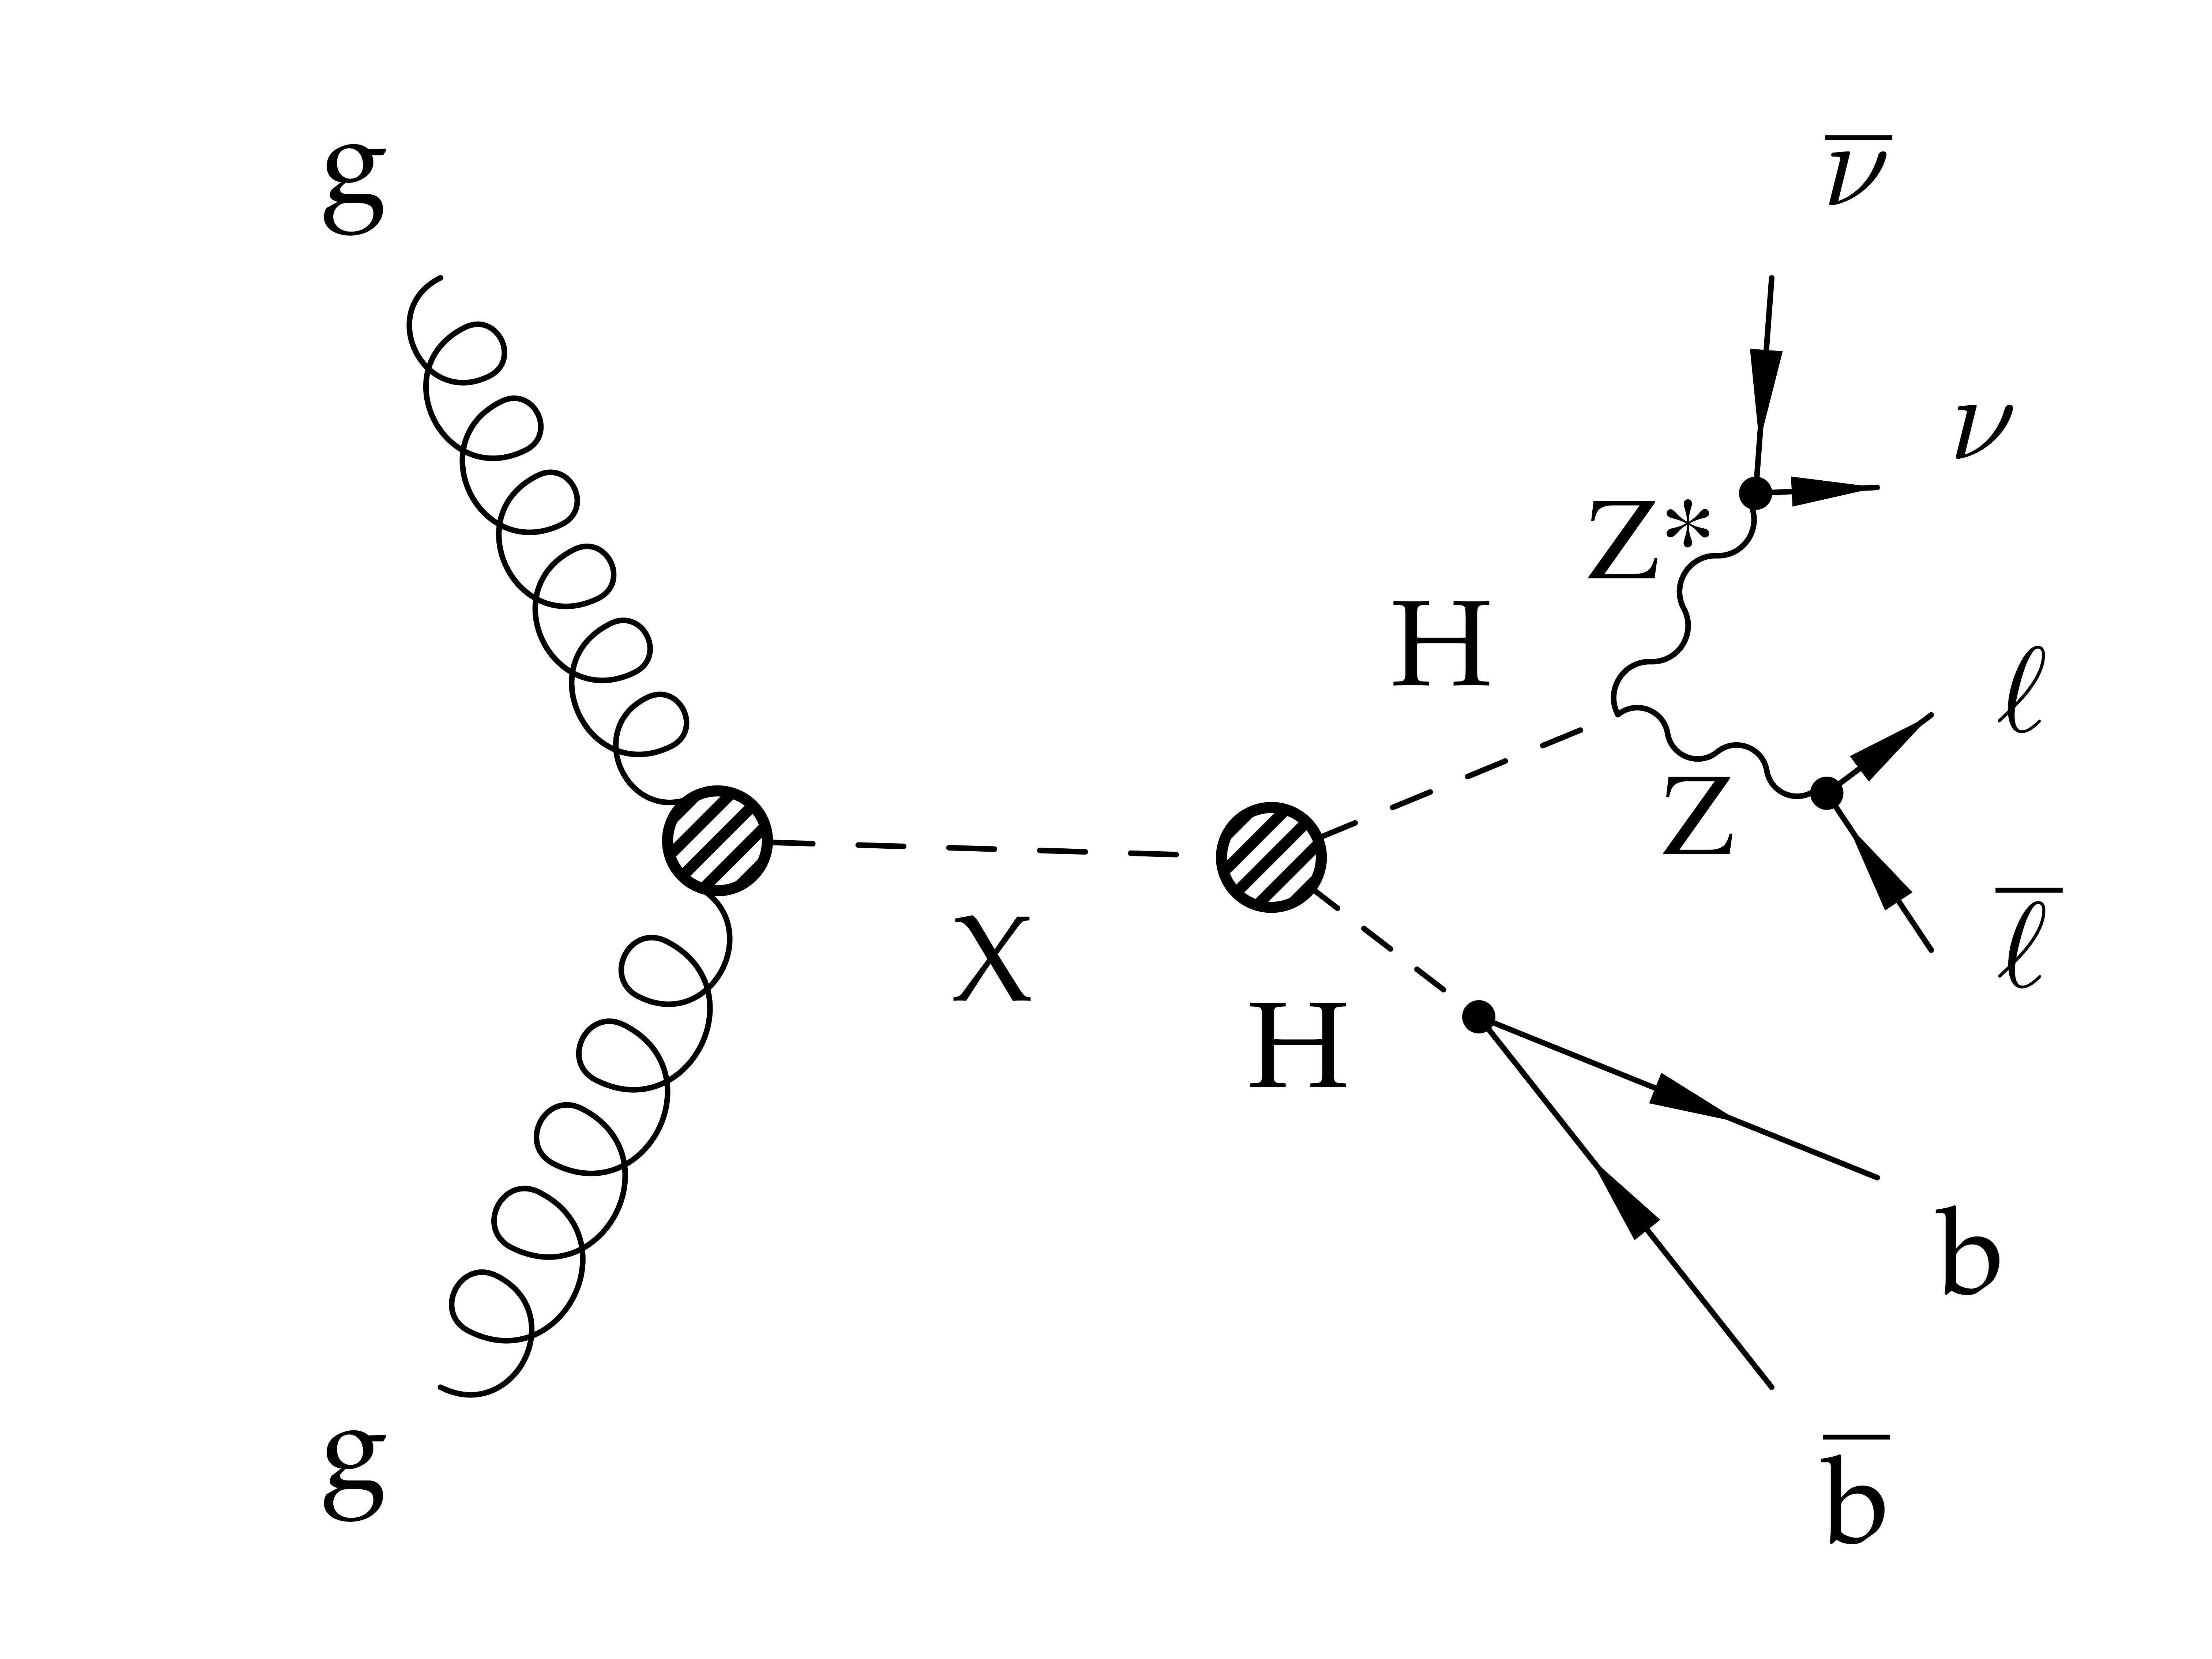
\includegraphics[width=0.50\textwidth]{HH_signature.png}
    \caption{BSM Resonant double Higgs decay in the 2 b, 2 lepton, and 2 neutrino final state. X denotes either graviton or radion particles. }
    \label{HH_signature}
\end{figure}




This thesis separately addresses both resonant graviton and radion decays into two SM Higgs bosons with the subsequent decays of one Higgs boson to a pair of b quarks, and the other Higgs boson to W or Z boson pairs. We select only leptonic W bosons decays. For Z boson decays, the chosen signature is characterised by the on-shell Z boson decaying into a pair of charged leptons and the off-shell Z boson decaying to neutrinos (see Fig. \ref{HH_signature}). The final state that this thesis focuses on consists of two b quarks, two charged leptons, and two neutrinos. Decays of the double Higgs system to this signature are observed on average in $2.8 \%$ of all di-Higgs decays. 


To finish this chapter, it is instructive to show all the decay channels of the double Higgs system to the SM particles, which are summarised in the Fig. \ref{BR}. Both the horizontal and the vertical axes show decays of a single Higgs boson to two SM particles. In this representation, each square on the plot specifies a branching fraction of one of the double Higgs boson decays, with the probability of the decay given by the color field map on the right axis. Our signature corresponds to 4 $\%$ of all $bbZZ$ decays, which are denoted on the map by the photo of the main $bbZZ$ analyser. 

\begin{figure}[H]
  \centering
    \includegraphics[width=0.50\textwidth]{BR2}
    \caption[Double Higgs decay channels]{Double Higgs decay channels. The SM branching fractions are represented by the color palette. In this measurement $bbZZ$ decays are analysed, which are denoted on the map by the photo of the main $bbZZ$ analyser.}
    \label{BR}
\end{figure}






%\setcounter{chapter}{2}

%    https://tex.stackexchange.com/questions/40725/how-to-change-the-font-size-during-the-new-defined-environment
%    http://www.sascha-frank.com/latex-font-size.html
%\begin{normalsize}
\begin{small}
%\begin{footnotesize}



\chapter{LHC and the CMS experiment}
\label{ch:cms}
CERN accelerator complex is a sequence of machines that produces and accelerates "bunches" of $10^{11}$ protons to nearly the speed of light. In the Large Hadron Collider (LHC) the bunches collide at specific interaction points (IP), where the four main experiments are located: ALICE, ATLAS, CMS, and LHCb. We will start this section with the discussion of the LHC machine and then describe the CMS detector. 

\section{The Large Hadron Collider}\label{sec:cms_intro}

%%%%%%%%%%%%%%%%%%%%%%%%%%%%%%%%%%%%%%%%%%%%%%%%%


\subsection{The history of the LHC}

The story of the LHC begins in 1977, when the CERN director general Sir John Adams suggested that the tunnel of the Large Electron-Positron Collider (LEP) can be reused to accommodate the future hadron collider of more than 3 TeV energies \ref{Sadenius}. At the 1984 ECFA-CERN workshop on a "Large Hadron Collider in the LEP Tunnel" \ref{LHC1984}, the physics goals of the LHC were stated: confirmation of the BEH mechanism, search for the Higgs Boson, and exploration of the origin of masses of W and Z bosons. The parameters of the proposed LHC were very ambitious: the centre-of-mass (COM) collision energy of 10 to 20 TeV, and a target instantaneous luminosity of 10$^{33-34}\frac{1}{cm^{2}s}$. 

Large Hadron Collider (LHC) is the most powerful particle accelerator that has ever been built. It is located at the border of France and Switzerland at a depth from 50 to 175 m underground. LHC ring is 26.7 km in circumference and it is the final stage in a sequence of accelerators. We will discuss the whole sequence of accelerators in the following section.



\begin{figure}[H]
  \centering
%  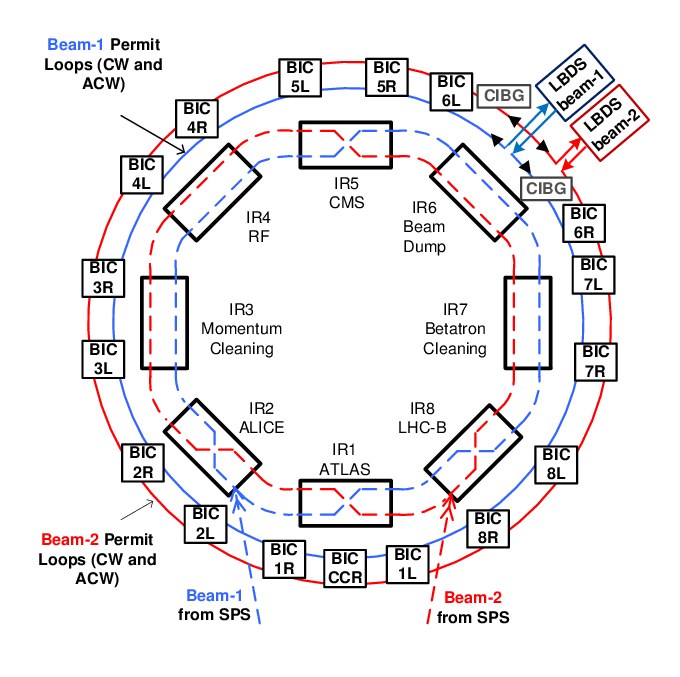
\includegraphics[width=0.75\textwidth]{LHC-beam-permit-loops}\\
  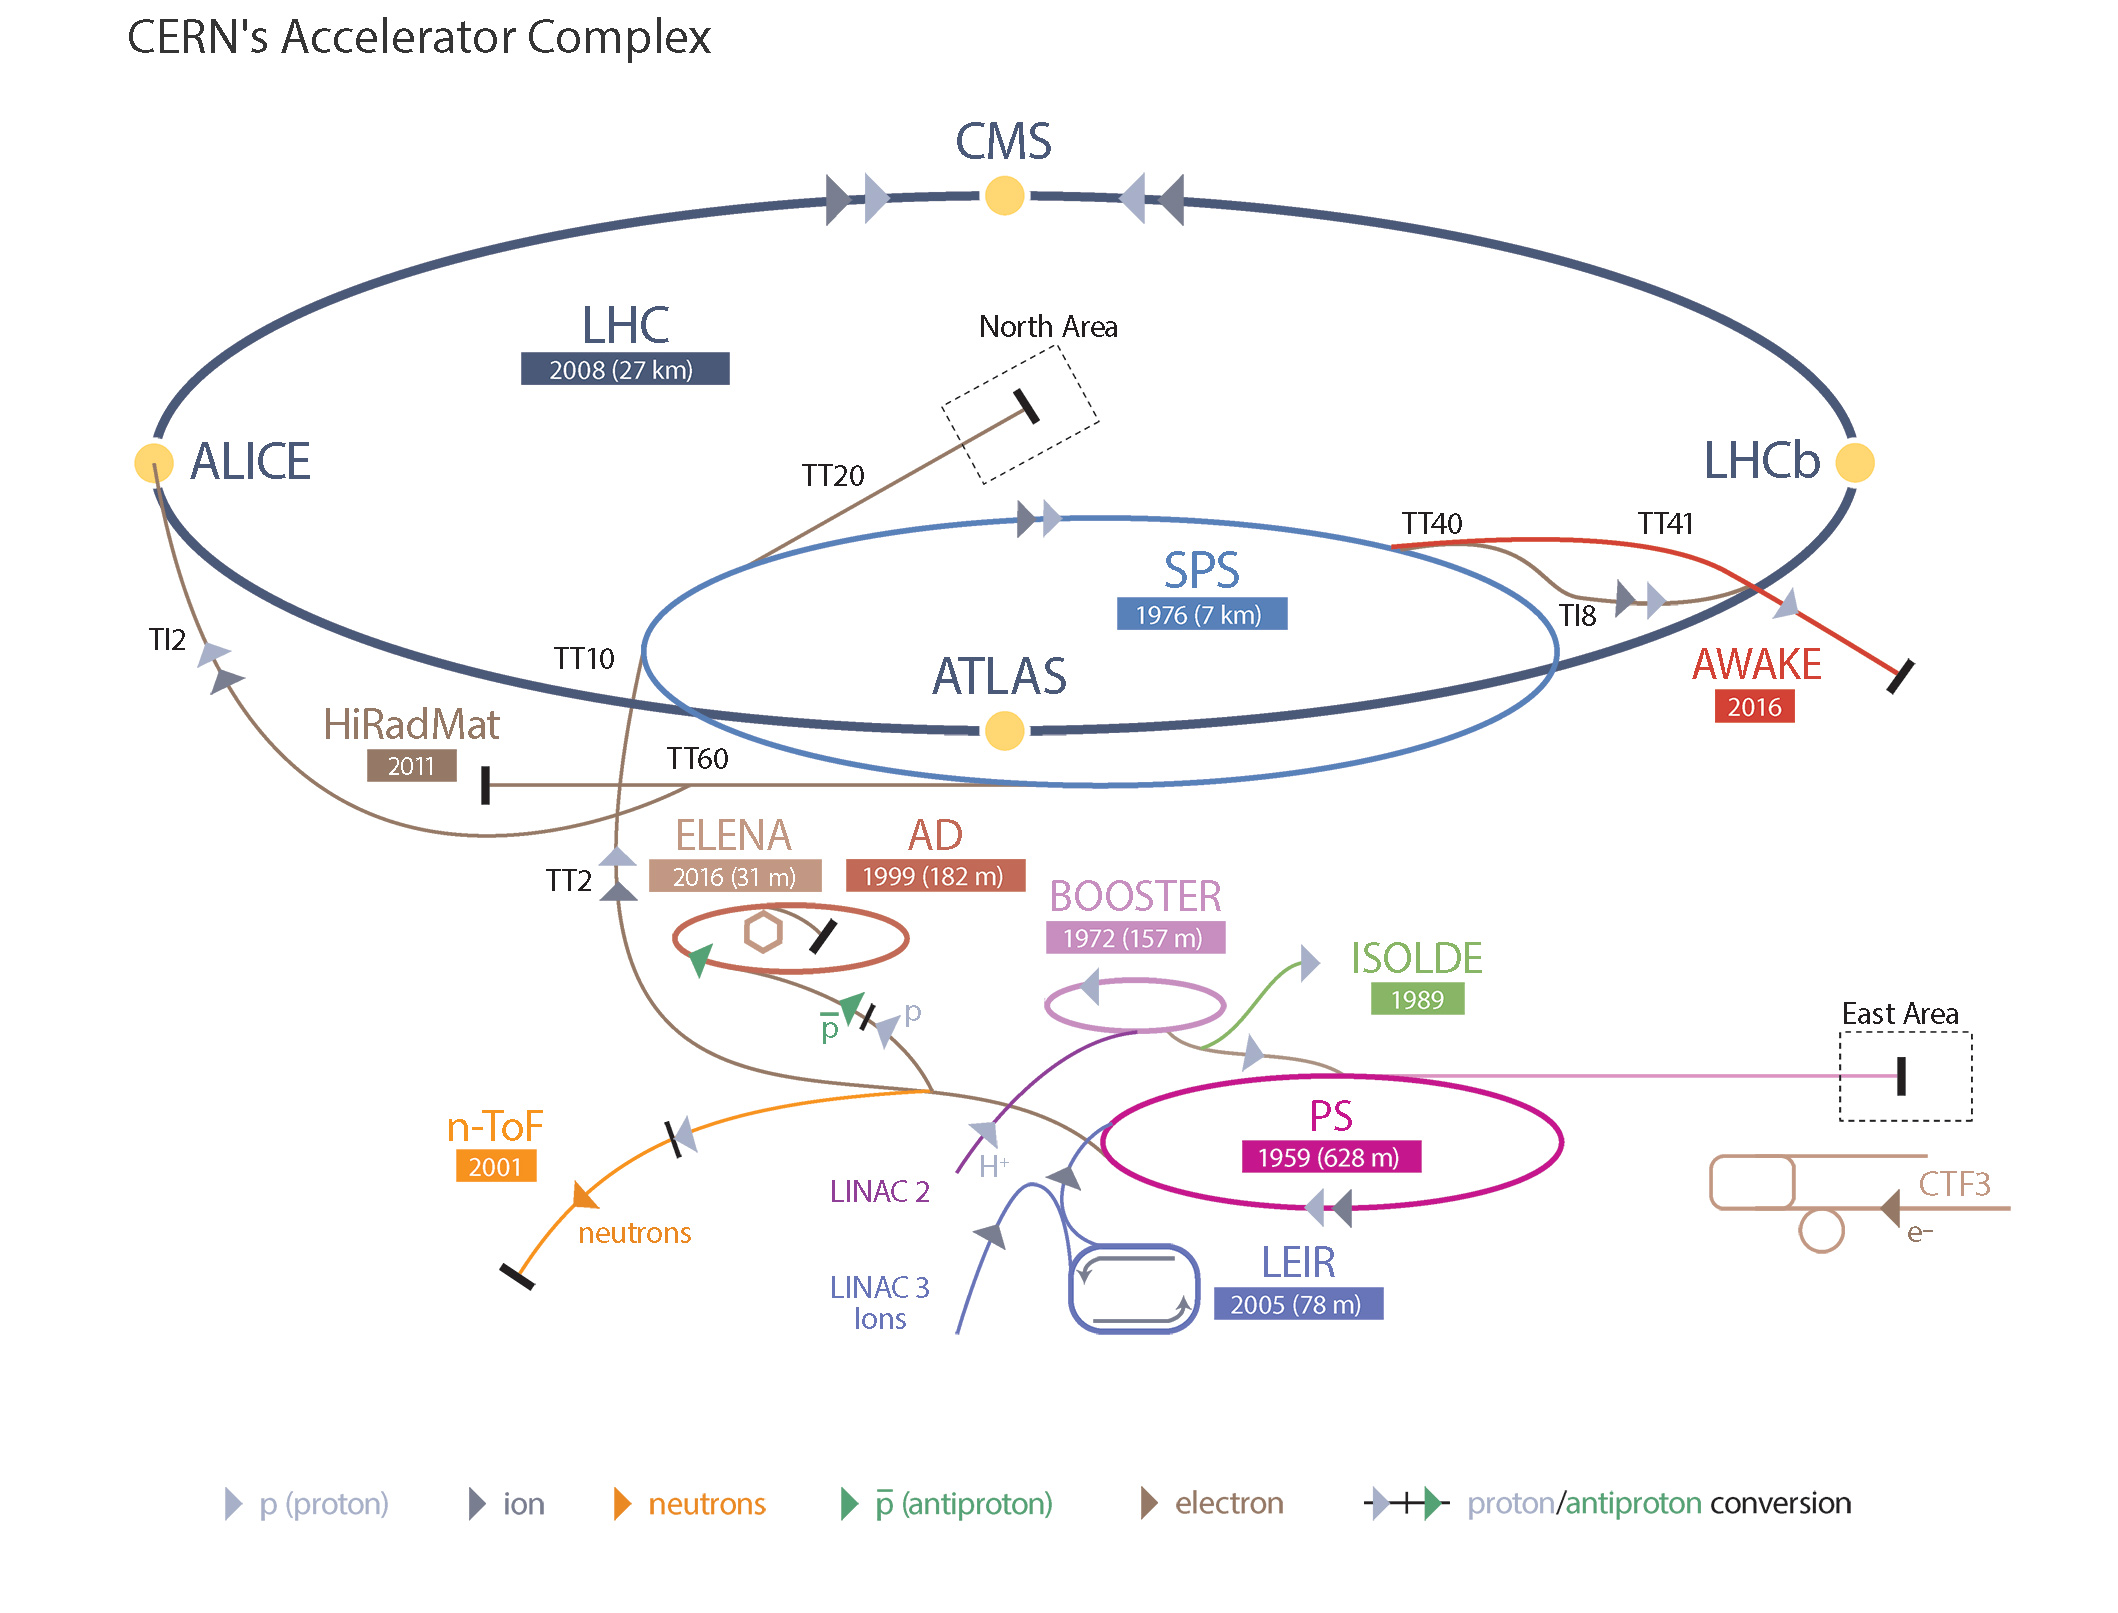
\includegraphics[width=0.75\textwidth]{LHC_default.jpg}
  \caption {Schematic layout of the LHC.}
  \label{lhcmap}
\end{figure}

%%%%%%%%%%%%%%%%%%%%%%%%%%%%%%%%%%%%%%%%%%%%%%%%%


\subsection{The layout of the LHC}

It is a complex process to start proton-proton collision in the LHC at 13 TeV and, therefore, the process consists of several stages (see Fig. \ref{lhcmap}). Everything begins with the bottle of hydrogen. The hydrogen atoms from the bottle are fed into the source chamber of the Linear Accelerator (Linac). In the chamber the hydrogen is heated up to the plasma state until electrons are stripped off of the hydrogen atoms. Then electrons are removed and remaining protons are directed to the first acceleration stage which increases the energy of protons to 50 MeV. After Linac, the beam of protons is injected into the Proton Synchrotron Booster (PSB). PSB contains four rings each accelerating a bunch of protons (a moving collection of protons of a narrow length) to 1.4 GeV. The third stage is the Proton Synchrotron (PS), which splits the incoming beam into 72 bunches separated by 7.5 m. The energy of the protons is increased to 25 GeV. After that, the protons are sent to the Super Proton Synchrotron (SPS), where they are accelerated to 450 GeV. SPS then fills the LHC ring with two beams each consisting of 2808 bunches of protons with nearly $10^{11}$ protons in total. It takes SPS about $O(10)$ minutes to fill each LHC ring with bunches. In the LHC two beams are circulating in opposite directions in two separate beam pipes. During standard data taking beams circulate for $O(10)$ hours.  

%%%%%%%%%%%%%%%%%%%%%%%%%%%%%%%%%%%%%%%%%%%%%%%%%

\subsection{LHC operations}

The first LHC budget plan was finalised in 1996 and the final cost was approved just a few years later. The first proton beam entered the LHC ring in 2008. However, an incident intervened the LHC plans. It was caused by the mechanical damage of the tunnel equipment due to the release of the helium. Thus, the real data taking period (called LHC Run-1) had started only in 2010, lasted for two years, and 7-8 TeV COM energies were used. The recorded dataset contained enough Higgs bosons to claim a discovery of this rarely produced particle. After this achievement, the LHC was closed for the first long shutdown (LS1) that happened in 2012. During this time necessary upgrades of the main detectors and the LHC were performed. This was an unavoidable and essential step to prepare the LHC for more challenging environment of COM energies increased to 13 TeV. 


If we denote the area of 10$^{-28}$ $m^2$ as barn (b), with the femtobarn ($fb$) equal to 10$^{-43}$ $m^2$, then in terms of these new units the LHC can theoretically produce $80-120/fb$ (inverse femtobarns) of data a year. In practice numbers were lower, because LHC operated at the revolution frequency below the nominal, used fewer proton bunches in the beam, etc.  All this resulted in lower than expected instantaneous luminosity, which is a very important term in collider physics and will be explained in the next section.

The LHC Run-2 has started in 2015 and the CMS collected 4.2 $fb^{-1}$ of data that year. Over the course of the 2016 data taking, an integrated luminosity of 35.9 $fb^{-1}$ was recorded. This luminosity is the amount of data that has been collected by the CMS detector and later approved by the CMS physics coordination for the use in the physics analyses. The data set of proton-proton collisions collected in 2016 at 13 TeV COM energy is used in this thesis to analyse double Higgs boson decays. Together with the 2017 and 2018 data taking, almost 150 $fb^{-1}$ have been delivered and recorded by the CMS detector during the whole Run-2 period of four years. 

At the moment of writing this thesis, the LHC has entered the LS2. The next data taking will resume in 2020 and proton-proton collisions will continue for three years with the expected delivered integrated luminosity equal to nearly 300 $fb^{-1}$. This will conclude the LHC Phase-1 programme. 

The new upgraded LHC, the High-Luminosity LHC (LHC) or the Phase-2, will start operations in 2026 and run until 2035. The COM energy will be increased to 14 TeV and one expects to record an unprecedented dataset of 3000 $fb^{-1}$. 

\subsection{Luminocity}

%%%%%%%%%%%%%%%%%%%%%%%%%%%%%%%%%%%%%%%%%%%%%%%%%

The instantaneous luminosity $ \mathcal{L} $ is the coefficient which relates the cross section $\sigma$ of the process to the number of events $N_{events}$ produced during the interaction: $N_{events} = \mathcal{L}  \sigma$. Luminosity is the parameter controlled by the machine and can be written as:

$ \mathcal{L} =\frac{N^2 n_b f_{rev}}{4\pi \sigma_x \sigma_y}$

\noindent where $N_b$ is the number of particle in the colliding bunch, $n_b$ is the number of colliding bunches in the beam, $f_{rev}$ is the revolution frequency of the beam, $\sigma_x$ and $\sigma_y$ are the standard deviations of the beam density profile (BDP) in the transverse plane, where it is assumed that the BDP of both beams can be described by a Gaussian distribution.


To maximise the amount of collected data, the luminosity parameter should be as high as possible. It is worth noting that the luminosity is not constant and decays with time due to the degradation of the initial circulating beams. Theoretical decay time (the time to reach $1/e$ level) is approximately 29 h. In practice, taking into account the decrease of protons in the bunch due to collisions, contributions from the intrabeam scattering, scattering on the residual gas, etc., the real luminosity lifetime is about 15 h. 

A useful variation of the luminosity parameter is a total integrated luminosity. This is the number normally quoted for the dataset collected over the period T:

$L = \int_{0}^{T} \mathcal{L}  dt$.

In collider physics the "beam dump" is a process of burning off exhausted low luminosity beams by intentionally directing them towards the target made of concrete and steel. The time from the start of the collisions to the beam dump is usually called the "run".

We can calculate the amount of data delivered by the LHC during a single run period $O(10)$ h. Performing the integration, we obtain: 

 $L = \mathcal{L}_0 \tau_\mathcal{L}  \left[  1- e^{\frac{-\tau_{run}}{\tau_\mathcal{L} }}  \right]$, 

\noindent where $\mathcal{L}_0$ is the initial peak instantaneous luminosity at the start of the run, $\tau_{run}$ is the total duration of a run, and $\tau_\mathcal{L}$ is the luminosity lifetime. The optimum run time is 12 hours. During the runs, the LHC centre needs to dump the old beams, fill the rings with the new beams, and increase ("ramp") the energy of new beams to 13 TeV. After that a new run can be started. This restarting process normally takes two to six hours.

%%%%%%%%%%%%%%%%%%%%%%%%%%%%%%%%%%%%%%%%%%%%%%%%%


\subsection{LHC infrastructure}

The equipment of the LHC tunnel serves several purposes with the main objective to keep the colliding beams on the circular orbit. This requires a complex synchronised work of bending dipole magnets, cooling systems, accelerating radio frequency cavities, and vacuum insulation systems.

%%%%%%%%%%%%%%%%%%%%%%%%%%%%%%%%%%%%%%%%%%%%%%%%%

\subsubsection{Magnets}\label{sec:magnets}

Most of the LHC circumference is used by 1232 superconducting magnets placed evenly around the tunnel to approximate the circular orbit. These are dipole magnets (see Fig. \ref{dipoles_coils}) that bend the beam and keep it on the circular orbit, that is why they are commonly called "Main Bends" (MB). The proven technology existed since Tevatron and relied on NbTi superconductors. This technology also satisfied the LHC cost and performance requirements, thus, it was decided to reuse the same choice of the alloy for the LHC superconducting dipole magnets that steer the proton beams. 

The dipoles need to produce the magnetic field of 8.3T. % and it requires a current of about 11kA. 
Each dipole is 16.5 $m$ (with ancillaries) long and 570 $mm$ in diameter and is placed inside of the dipole cryostat which is called the "Helium bath". 

This cryostat is a long cylindrical tube 914 $mm$ in diameter made of low-carbon steel, where the dipole mass is cooled down to 1.9 $K$. Even though the inner structure of such cryostat is very complex and includes two beam pipes, two sets of coils for two beam pipes, vacuum pipes etc., one normally calls this compound object simply a dipole magnet. The name "dipole" is reserved for MBs since for each beam pipe the magnet consist of two "poles" that provide a vertical magnetic field similarly to a simple dipole system of magnets. 

\begin{figure}[H]
\centering
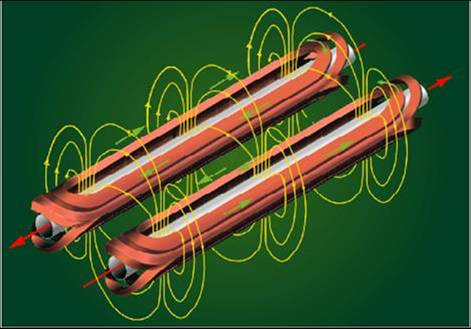
\includegraphics[width=0.65\textwidth]{dipole_1.jpg}\\
\vspace{0.5cm}
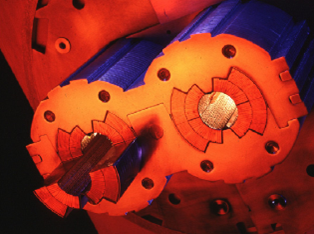
\includegraphics[width=0.65\textwidth]{dipole_2.png}
\caption[LHC dipoles]{LHC dipole magnets. Top: two dipole coils and magnetic field lines. Bottom: two beam pipes with the coils inside of the dipole magnet. }
\label{dipoles_coils}
\end{figure}



A  dipole magnet  must  be  curved to help a chain of dipoles complete 360 degrees. The curvature is 5.1 $mrad$ per dipole, which is equivalent to a  sagitta of  about  9 mm, corresponding to a radius of curvature of 2812.36 m.


The other important set of magnets is quadrupoles. They are used to ensure the proper beam dynamics. In total 392 quadrupole magnets ranging from 5 to 7 metres in length are used to squeeze the beam in transverse direction and to keep it narrow during the run duration. Additional special quadrupole magnets (SQM) are installed right before the IPs to focus the beams even more. That increases the density of protons in the beam and guarantees the maximum luminosity. In addition, SQMs help to decrease the chance of the parasitic collisions when bunches from the same beam or bunches outside of the IP centre interact (see Fig. \ref{quadrupoles}). To further correct the beam path (orbit), about 5000 higher order correcting magnets are used, which are evenly spaced around the circular trajectory of the LHC. 


\begin{figure}[H]
\centering
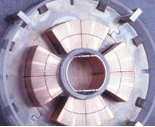
\includegraphics[width=0.4\textwidth]{quad_2.png}
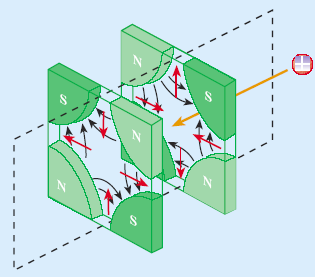
\includegraphics[width=0.37\textwidth]{quad_1.png}\\
\vspace{0.5cm}
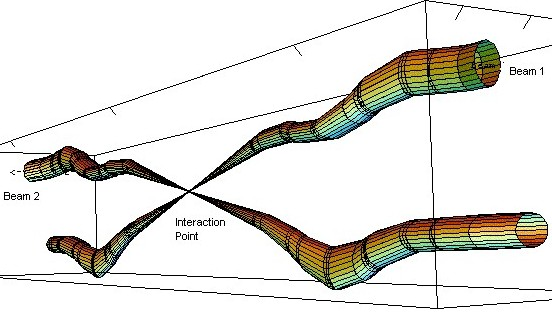
\includegraphics[width=0.7\textwidth]{quad_3.jpg}
\caption[LHC quadrupoles]{LHC quadrupoles. Top left: the coil of the quadrupole magnet. Top right: schematic view of the magnetic fields in the quadrupole. Bottom: two beams and the IP.}
\label{quadrupoles}
\end{figure}


To power the LHC, 1612 electrical circuits are used. Mostly these circuits are needed to power the dipole and quadrupole magnets, which is done in eight evenly spaced location of the LHC. A total of 3286 current leads are needed to connect all the circuits and power cables. More than a thousand of the leads operate between 600 A and 13 kA (see Fig. \ref{13kA_lead}). The other leads operate in the range 60 to 120 A. 

\begin{figure}[H]
  \centering
  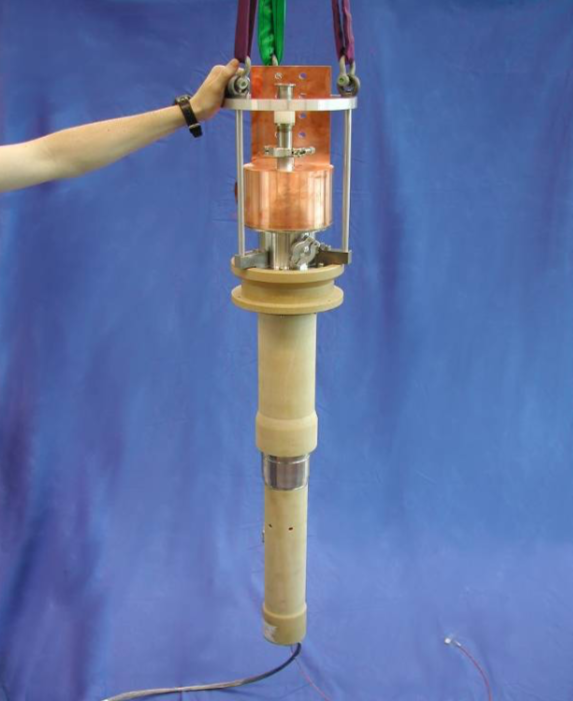
\includegraphics[width=0.5\textwidth]{13kA_lead}
  \caption{13 kA high-temperature superconducting current lead.}\label{13kA_lead}
\end{figure}


%%%%%%%%%%%%%%%%%%%%%%%%%%%%%%%%%%%%%%%%%%%%%%%%%

\subsubsection{Cooling System}\label{sec:cryogenic}

To ensure that dipoles are in the superconducting state, they have to be cooled to 1.9 K using superfluid helium-4. 

The cooling (cryogen) system is needed to keep superconducting LHC magnets at the appropriate temperature. The choice of the cooling gas depends on the magnet type and location. This dictates the required range of temperatures, which differs from system to system by 75 K. The cryogen system uses layered design with the temperature becoming progressively colder going from outside the dipoles closer to the beam pipe. 

The "coldest" part of the cryogen system is designed for the inner part of the dipoles. This system (see Fig. \ref{cryo_T_scale}) must cool down 37 Mkg of the LHC magnets within 15 days to the required temperatures, which is done through the system of pipes that transports and directs the flow of the superfluid helium. The cryogen system must also be able to deal with the fast increases of the pressure flow and flow surges, as it is crucial for the LHC operation to keep dipoles constantly cooled and at the superconducting state.


The LHC tunnel is inclined in the horizontal plane by 1.41$^\circ$. This translates to 120 m difference in the vertical location of two diametrically opposite points of the tunnel with respect to the surface level; and results in the additional hydrostatic pressure that can affect the flow of helium. This has been an important concern during the design of the cryogen system.


Since the cost to cool the LHC equipment to 1.8-1.9 K temperatures is high, several temperature levels are employed (see Fig. \ref{cryo_T_scale}):
 
\begin{itemize}
\item 50 to 75 K for the thermal shielding used in the dipoles,
\item 20 to 300 K for upper ("warm") sections of the high-temperature superconducting current leads,
\item 4.6 to 20 K for lower temperature interception,
\item 4.5 K for radio frequency cavities and lower ("cold") sections of the high-temperature superconducting current leads,
\item 4 K for the transportation system that directs the 1.8 K helium to dipoles,
\item 1.9 K for helium in the superfluid state to cool magnet masses.
\end{itemize}

\begin{figure}[H]
  \centering
  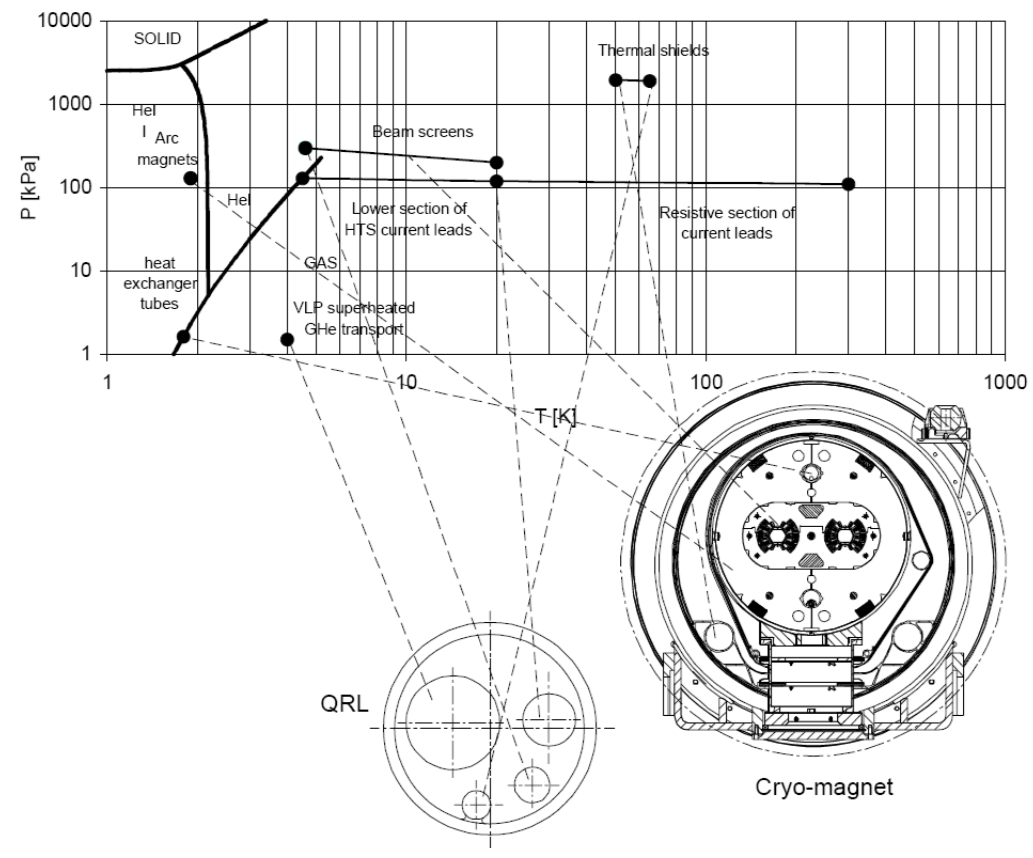
\includegraphics[width=0.7\textwidth]{cryo_T_scale}
  \caption{LHC cryogenic states and the temperature scale.}
  \label{cryo_T_scale}
\end{figure}


%%%%%%%%%%%%%%%%%%%%%%%%%%%%%%%%%%%%%%%%%%%%%%%%%


\subsubsection{Radio Frequency Cavities}\label{sec:rf}


Proton bunches need to be ramped to 7.5 TeV energies. To achieve this 13 TeV COM energy, eight superconducting radio-frequency cavities (RFC) are used per beam. They are located in front of the IPs of four experiments. Electromagnetic waves of 400 MHz with a peak field strength of 5.5 MV/m adjust the speed of protons in bunches. Each RFC (see Fig. \ref{lhc_rfc}) increases the energy of protons by 60 keV per revolution and it takes $O(20)$ minutes to reach 6.5 TeV beam energy. The RFC frequencies are increased gradually by 1 kHz to match the speed up of protons in the bunch as they gain more energy. When the ramp is completed, the RFCs are used to compensate for small energy losses due to the synchrotron radiation (7 keV per revolution). 




\begin{figure}[H]
\centering
%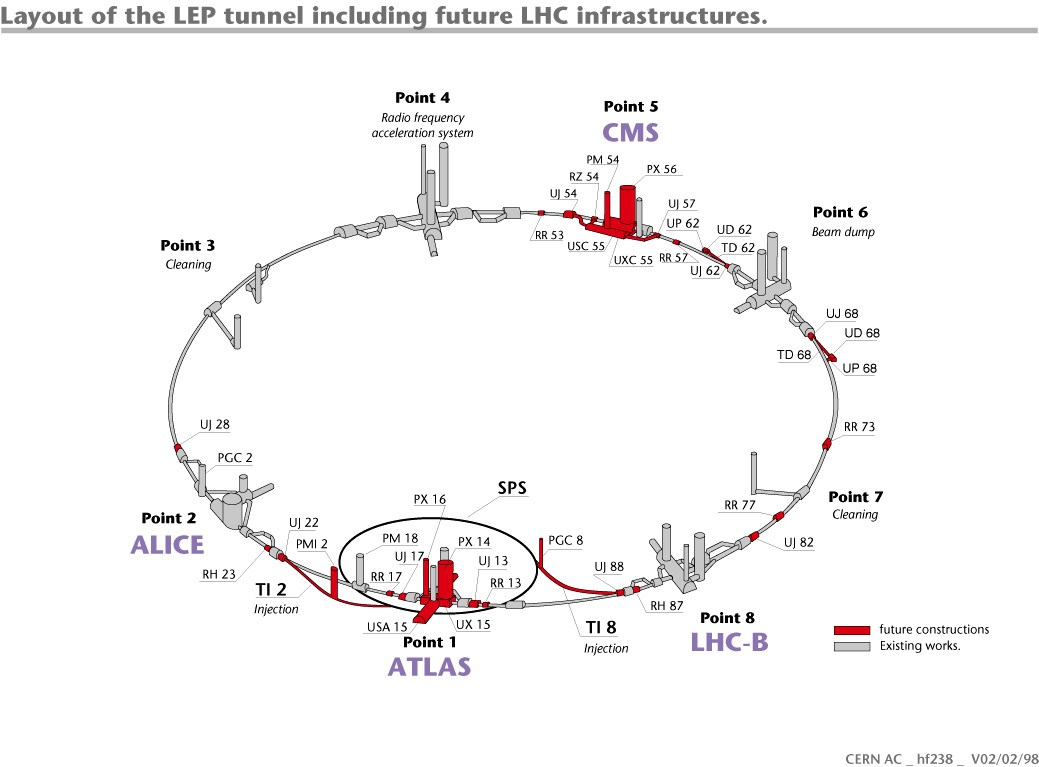
\includegraphics[scale=0.6]{lep}
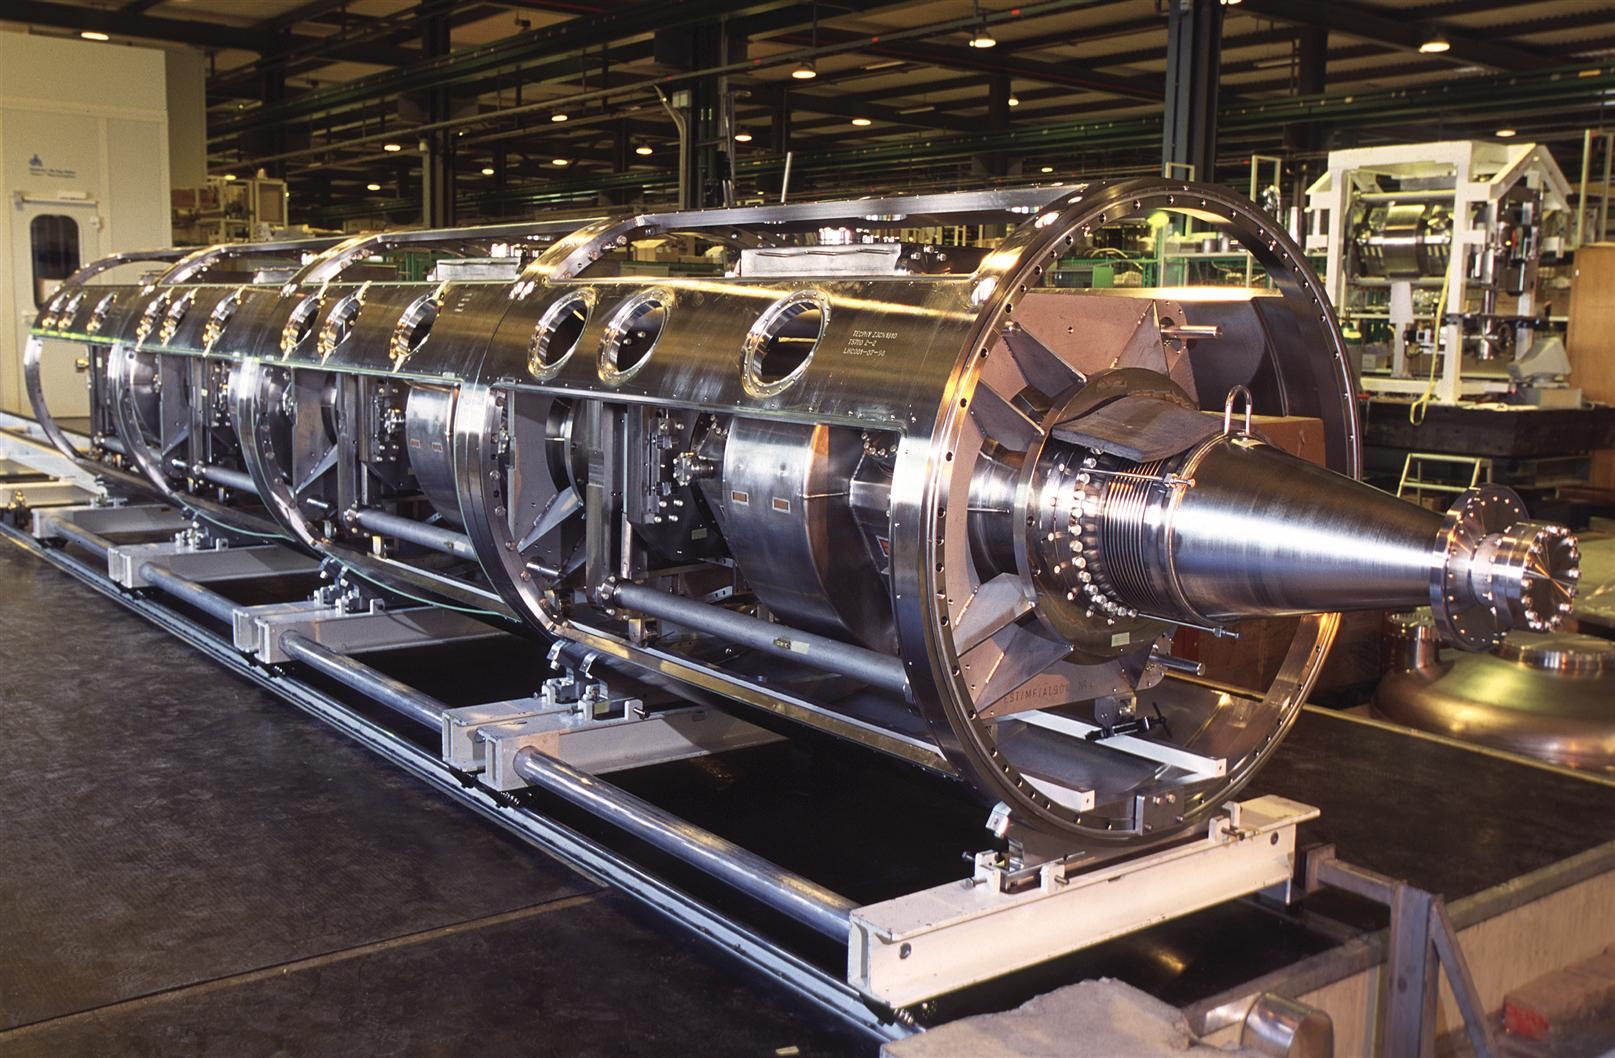
\includegraphics[width=7cm,height=4.2cm]{lhc_rfc}
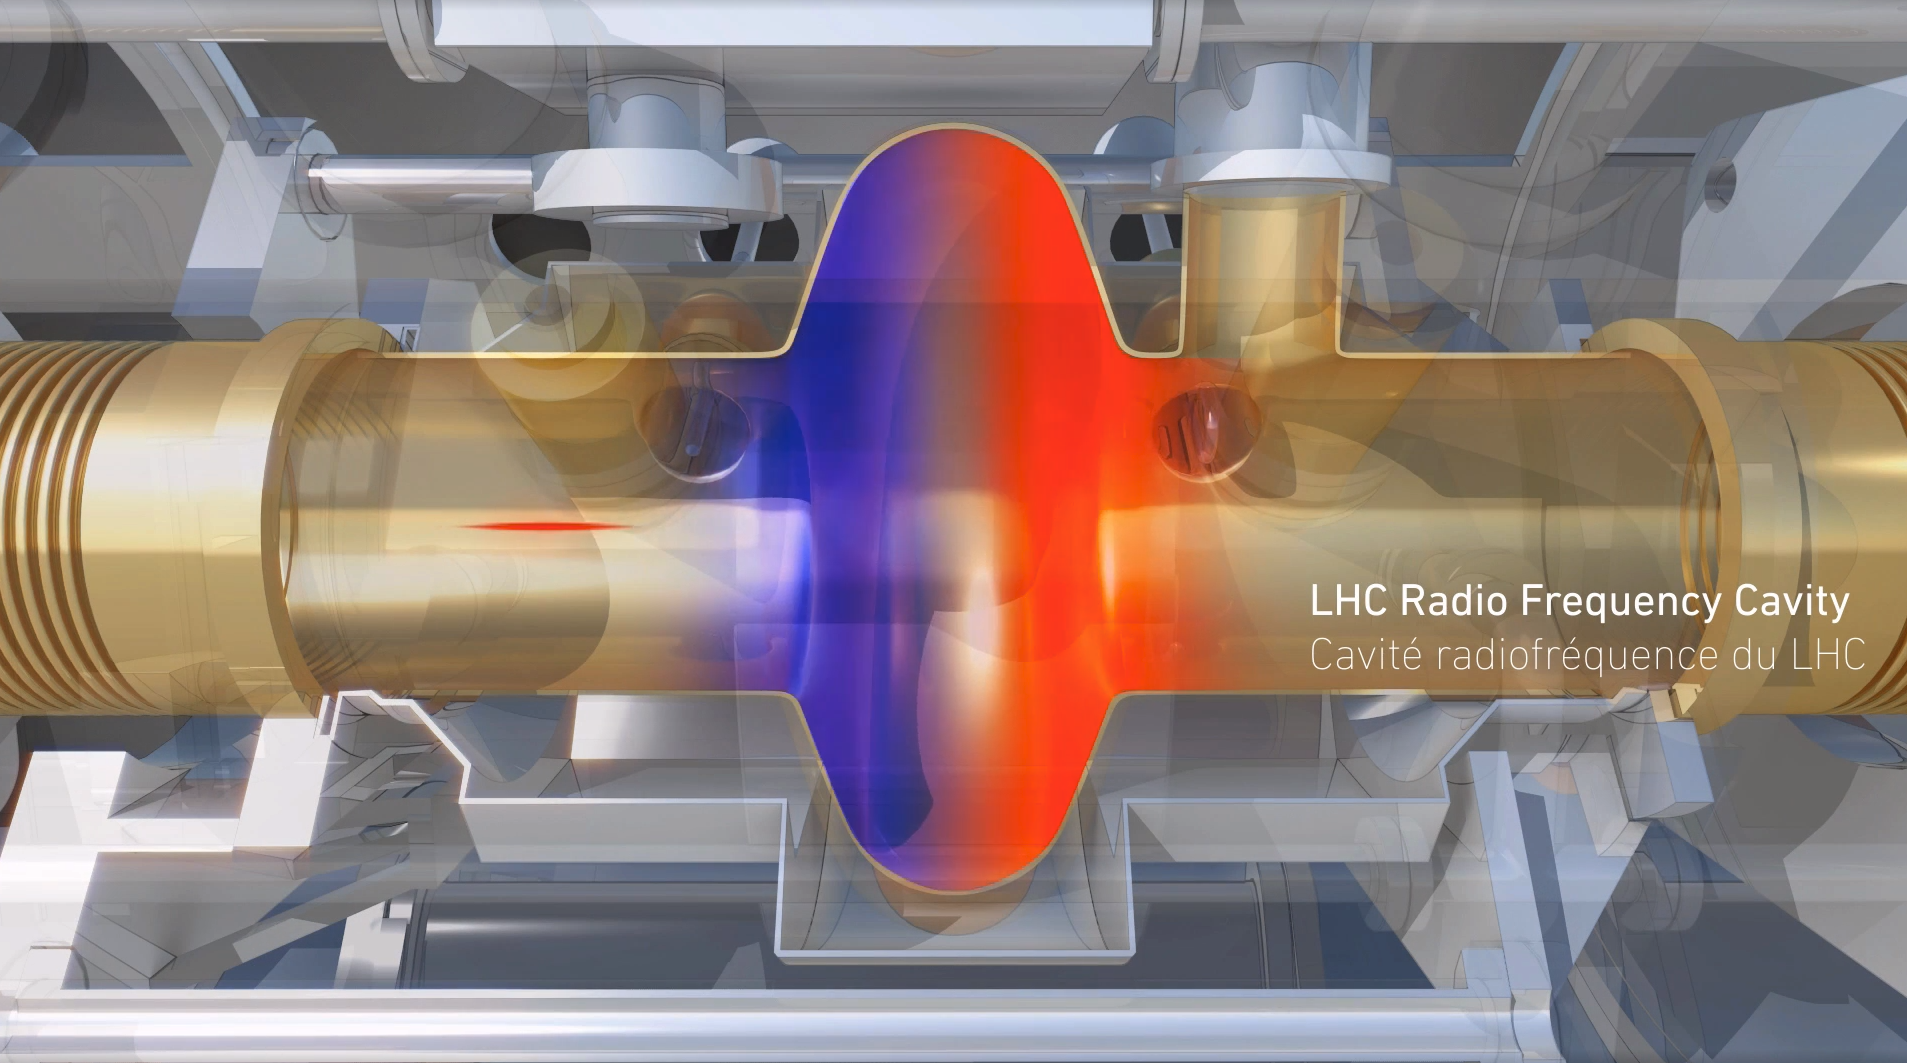
\includegraphics[scale=0.15]{rfc_lhc}
\caption[RF cavities module.]{LHC RF cavities. Left: a cryomodule with four RF cavities. Right: a schematic drawing of a single RF cavity. The colour field is used to denote positive (red) and negative (blue) polarities. A narrow beam traversing the cavity is coming from the left and is shown in red. }
\label{lhc_rfc}
\end{figure}


%%%%%%%%%%%%%%%%%%%%%%%%%%%%%%%%%%%%%%%%%%%%%%%%%


\subsubsection{Vacuum System}\label{sec:vacuum}



The work of the LHC depends on three vacuum systems \cite{LHC_vacuum}. Without them, dipoles will not be at the superfluid state, the beams will not be able to circulate, and no stable collisions would be taken. With a total of 104 kilometres of vacuum pipes, the LHC owns the largest vacuum system in the world. The main types of vacuum systems are:

\begin{itemize}
\item insulation vacuum for cryomagnets,
\item insulation vacuum for the helium distribution line,
\item beam vacuum.
\end{itemize}


The insulation vacuum is needed to ensure the operations at both low temperatures of the magnets and the room temperatures in the tunnel. The insulation vacuum of $10^{-6}$ mbar is used for a total of 15000 cubic metres. To build this vacuum system, the LHC used 250,000 welded joints and 18,000 vacuum seals. 


The vacuum for the helium distribution lines is needed to protect from the heat the flow of the helium-4. This helium flow is used to cool down the dipole mass. Cryogenic distribution lines (QRL) of 3.3 km each are connected to eight cryogenic plants that pump the helium-4 into the LHC. The vacuum in these systems is at $10^{-7}-10^{-10}$ mbar level. 



For the beam pipes the LHC uses ultra-high vacuum of $10^{-10}$ mbar at cryogenic temperature of 5 K. The vacuum is getting progressively closer to $10^{-11}$ mbar near the IPs, because in these locations collisions take place and any additional gas is highly undesirable. This vacuum is the emptiest space in the Solar System. This ultra-high vacuum is needed to reduce the beam degradation due to the beam-gas interactions in the pipe and parasitic collisions of bunches with the collimators near the IPs. 

Vacuum system are affected by the heat produced from the synchrotron radiation emitted by the proton beams when they are bent. To reduce the amount of this heat and to narrow down the beam size in the transverse direction when the beam widens, the LHC uses "beam screens", which operate between 5 and 20 K. 


\begin{figure}[H]
  \centering
  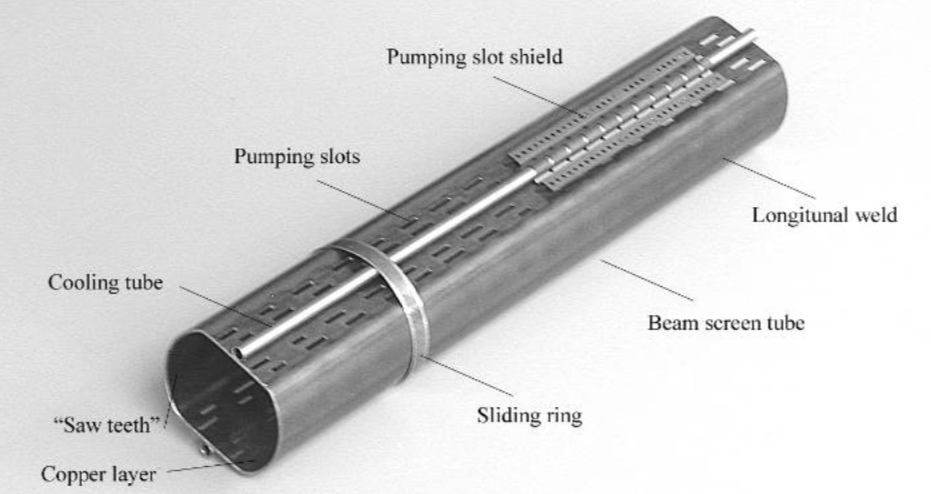
\includegraphics[width=0.7\textwidth]{beam_screen}
  \caption{Beam screen.}\label{beam_screen}
\end{figure}



The beam screens are necessary to reduce the number of protons scattering on the residual gas of the beam pipes, which could lead to a magnet quench and even interrupt the machine operation. 

The table below summarises the main heat sources that degrade the vacuum quality in the beam pipe, where the vacuum must exist at 1.9 K:


\begin{itemize}
\item synchrotron radiation (0.2 $W/m$ per beam),
\item energy loss by nuclear scattering (30 $mW/m$ per beam),
\item image currents (0.2 $W/m$ per beam),
\item electron cloud related effects (vary).
\end{itemize}



Now, that we discussed the LHC collider, we can continue with one of the main LHC detectors - the CMS detector - the one that was used to collect the data analysed in this thesis. 

%%%%%%%%%%%%%%%%%%%%%%%%%%%%%%%%%%%%%%%%%%%%%%%%%


\section{The CMS experiment}

                

The Compact Muon Solenoid (CMS) is a multi-purpose particle detector built to study a variety of complex particle interactions produced by the LHC. CMS is located in the underground cavern at the "Point 5", which is one of the four main IPs of the LHC. The CMS detector with the additional computing infrastructure is able to detect the produced particles, measure their main physics parameters, and to send the related data to computing data centres for persistent storage. 


The CMS detector has a cylindrical shape and consists of a central ("barrel") and two forward ("endcaps") sections (see Fig. \ref{CMS_detector}). 
CMS is the heaviest detector ever built with the mass of nearly 12500 tons. The mass is explained by the amount of the used superconducting metal, which serves as the magnet. The CMS is 21.6 m long and 14.6 m high. The CMS has an onion-like structure of concentric layer of detectors around the IP. In addition, at the outer part it has a large superconducting solenoid to produce inside the detector a homogeneous magnetic field of 3.8 T.

\begin{figure}[H]
  \centering
  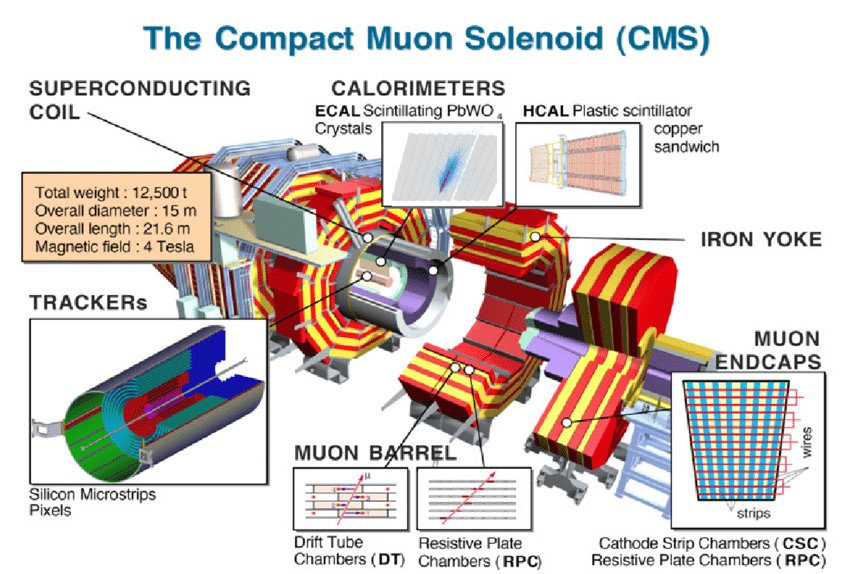
\includegraphics[width=0.8\textwidth]{CMS_detector}\\
  \vspace{1cm}
  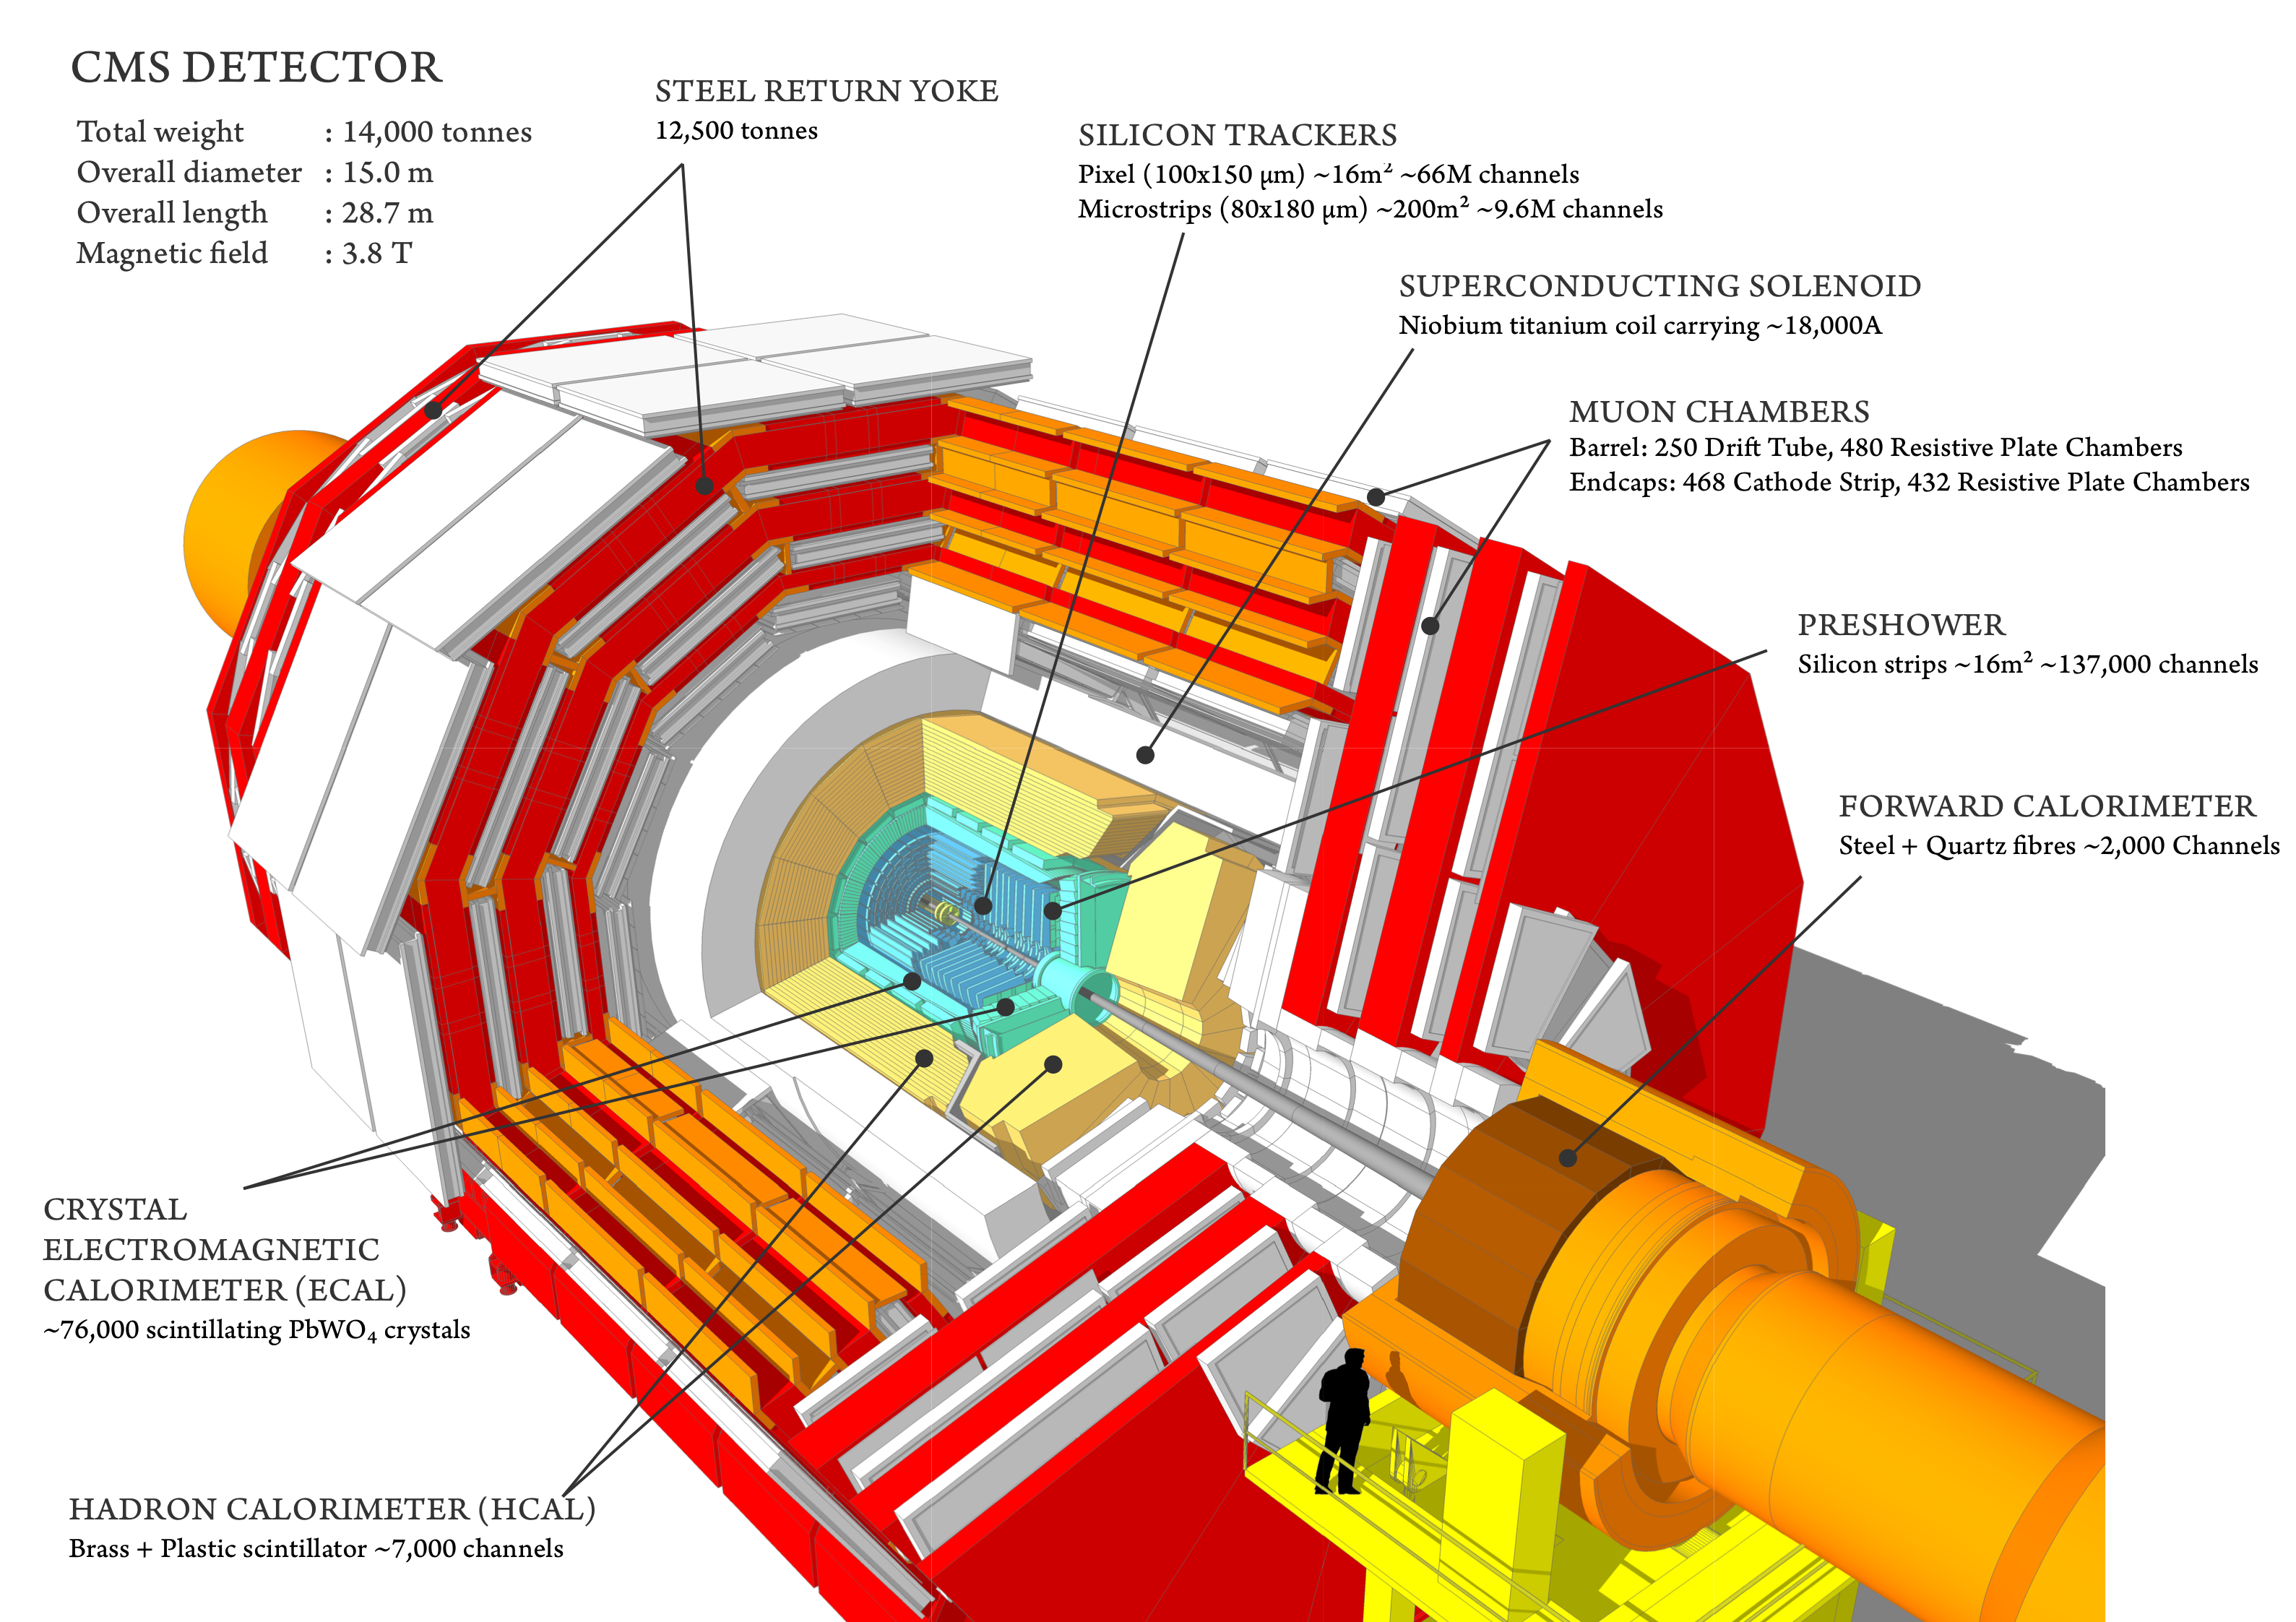
\includegraphics[width=0.8\textwidth]{cms_cross_section}
  \caption{CMS experiment with the main sub-detectors.}
  \label{CMS_detector}
\end{figure}


All sub-detectors can be categorised into trackers and calorimeters \cite{Hauptman:2011zza}. As the particle passes through the material of the tracker, it leaves a "track", which is a path of the emerging particle. Trackers focus on the direction and the track curvature of the charged particles. Tracking information allows the determination of the particle's momentum. 

There are two trackers in CMS: an inner tracking system that encloses the IP and the outer tracking system that is located outside of the solenoid magnet. The first system contains the Pixel and the Strip trackers. The second tracking system is dedicated for the muon detection and is usually called a muon tracker or a muon system. This system is embedded within a steel yoke of the magnet. 

The magnet yoke is made of five barrel wheels. Such an arrangement saves the CMS some space and also is used for the magnetic flux return. Additionally, it serves as a support for the embedded muon system, which is located outside of the ECAL and HCAL systems. Muons are energetic enough to traverse the ECAL and leave the detector. This muon system-magnet yoke structure provides a return field of the magnet of about 2 T and is used to measure the momentum of muons. This "two-directional" magnetic field with respect to the magnetic yoke, causes the muons trajectories to be bent in opposite directions in the inner tracker in contrast to the outer tracker. This important feature of the CMS detector is depicted in the CMS logo (see Fig. \ref{cms_logo}). 

\begin{figure}[H]
  \centering
  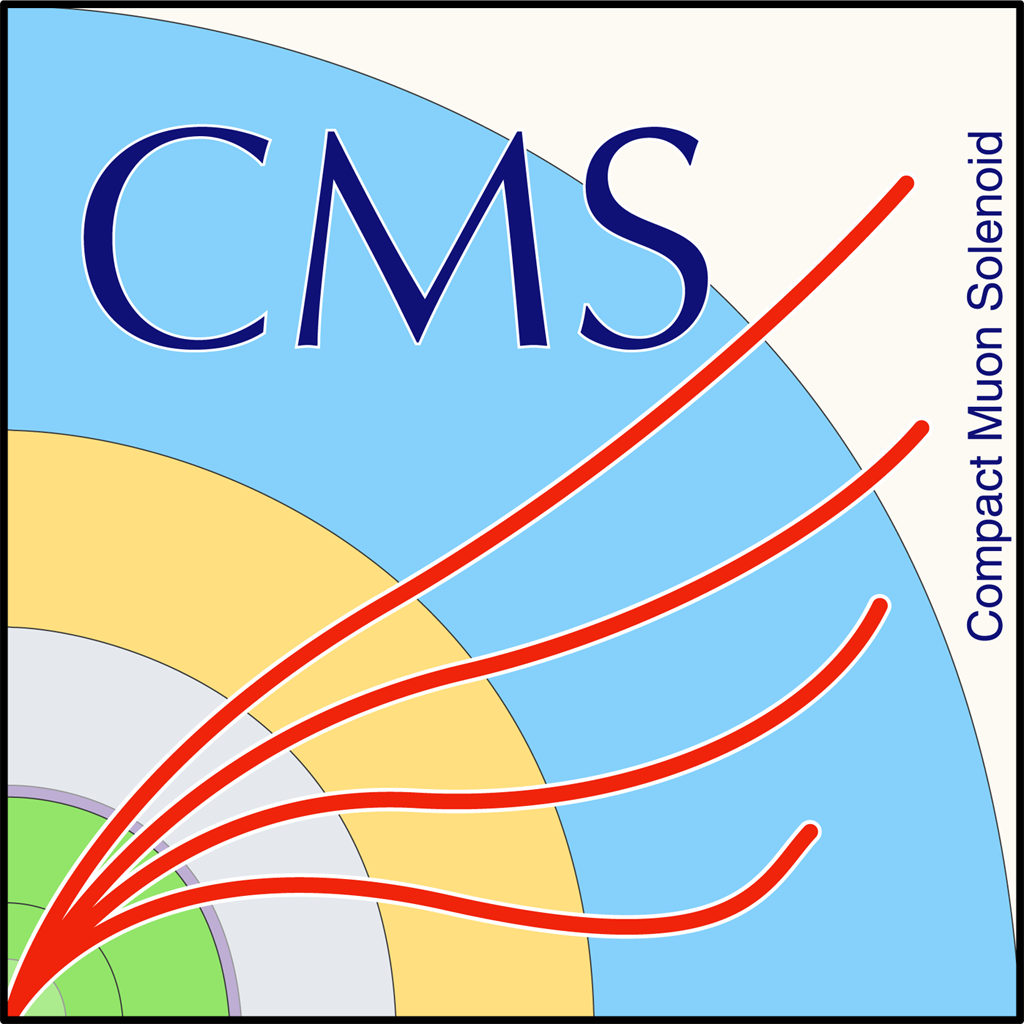
\includegraphics[width=0.4\textwidth]{cms_logo}
  \caption{The logo of the CMS experiment that is showing curved trajectories of the emerging muons.}
  \label{cms_logo}
\end{figure}


The CMS has two calorimeters: the electromagnetic and the hadronic calorimeters. They both rely on high density materials either to sample or to contain almost all the energy of the incoming particles with their secondary interaction products. However, these two systems focus on two different sets of particles. As will be discussed later, electromagnetic calorimeter (ECAL) is dedicated to measuring the energy of photons and electrons, while the hadronic calorimeter is targeting the measurement of the energy of hadrons.
1!
The rate of the incoming data at the LHC is 40 MHz. This corresponds to almost 70 TB produced every second! It is impossible to store that much data, and, most importantly, most of the information in this data is not interesting for future physics analyses. To reduce the data rate, the CMS uses a highly efficient system of triggers. The first one, the Level-1 (L1) trigger, reduces the nominal collision rate of 40 MHz to 100 kHz. The subsequent High-Level Trigger (HLT) further decreases the rate to 1 kHz. With the help of the trigger system, the original 40 TB per second rate is transformed into manageable 1 GB per second that is stored for offline analysis use. 

%%%%%%%%%%%%%%%%%%%%%%%%%%%%%%%%%%%%%%%%%%%%%%%%%


\subsection{The CMS coordinate system}

The CMS uses a a right-handed Cartesian coordinate system to define the axes of the colliding beams (see Fig. \ref{coord}). The centre is located at the IP and the x axis points to the centre of the LHC ring. The y axis points upwards, and the z axis points along the proton beam direction. Since the CMS detector has a cylindrical shape, the polar system is used in the x-y plane: a standard set of the azimuthal angle $\varphi$ and the radial coordinate $r$. The polar angle $\theta$ is defined in the r-z plane and a widely used in this thesis angular variable $\eta$ (called pseudorapidity) is defined as $\eta = \ln \tan(\theta/2) = \ln (\frac{\mid \vec{p}\mid + p_z}{\mid \vec{p}\mid - p_z})$. Additionally, a popular quantity in the collider physics - the rapidity - is given by $y = 1/2 \ln ( \frac{E + p_z}{E - p_z})$. Rapidity is a function of the energy E and longitudinal momentum $p_z$ of the particle (the projection of $\vec{p}$ on the z axis. 
Note that $\eta$ converges to $y$ when the mass is negligible and the particle travels with the speed close to the speed of light. Most angular variables that are used currently in the modern high-energy physics (HEP) are defined in terms of $\eta$ and $\varphi$:
$ \Delta R = \sqrt{(\Delta \eta)^2 + (\Delta \varphi)^2}$, with $\Delta \eta$ and $\Delta \varphi$ being the absolute values of the relative differences of $\eta's$ and $\varphi 's$ of two particles. 

Another extremely useful quantity is the projection of the momentum of a particle on the transverse plane and is called "transverse momentum" $p_T$. This variation of the momentum is independent of the z axis, hence, from the Lorentz boost.  Similarly, the "transverse energy" of a particle is defined as $E_T = \sqrt{m + p_T }$. 


\begin{figure}[H]
  \centering
  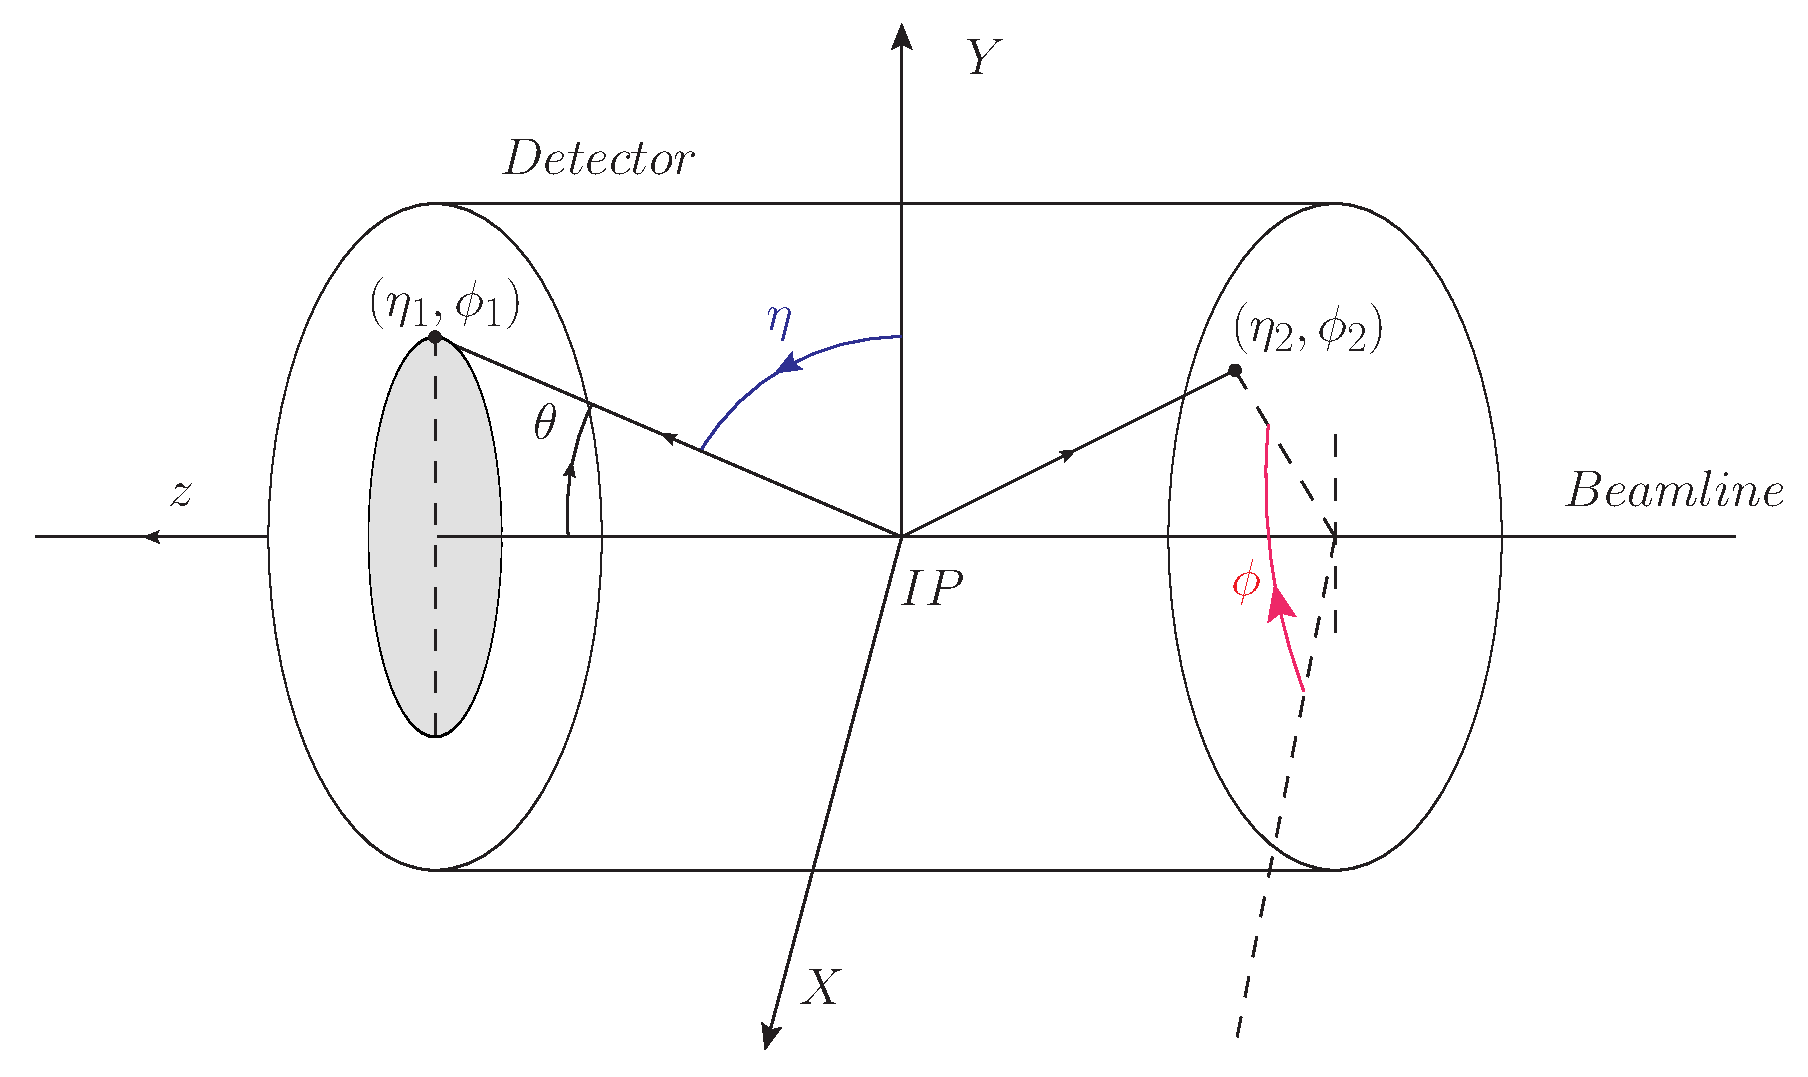
\includegraphics[scale=0.4]{coord}
  \caption[Coordinate system of the CMS detector]{Coordinate system of the CMS detector \ref{MonroyMontanez:2639240}. Two particles (1 and 2) are shown with the corresponding angular variables ($\Delta \eta_1$, $\Delta \varphi_1$) for the first and ($\Delta \eta_2$,$ \Delta \varphi_2$) for the second particle respectively.}
  \label{coord}
\end{figure}

%%%%%%%%%%%%%%%%%%%%%%%%%%%%%%%%%%%%%%%%%%%%%%%%%

\subsection{The Inner Tracker}

The inner tracker \cite{Tracker_phase2} (see Fig. \ref{inner_tracker}) is the closest subdetector to the IP. Using the tracker the experiment measures the trajectories of charged particles and reconstructs decay vertices. Since this system is constantly under the radiation coming from the interactions with the particle flux of nearly 100 MHz/cm at r = 4 cm, the design of the tracker focused on two main requirements: high granularity for precise determination of the vertices and tracks, and robustness against the radiation-hard environment with the operational time of at least 10 years. As a solution to both challenges, the CMS relies on the silicon technology that provides the tracker with the large surface of thin but highly granular active detectors. The tracking system has a diameter of 2.4 m and a length of 5.4 m covering the detector space of $|\eta|< 2.5$. 

The inner most part of the tracker - the Pixel detector ("Pixel")- consists of three layers in the barrel at the radii of 4.4 cm, 7.3 cm, and 10.2 cm respectively. The Pixel also has two detector disks in forward regions. They are positioned 34.5 and 46.6 cm away from the IP. The Pixel is made of 1440 modules which contain 66 million pixel cells. Each cell is 100 by 150 $\mu$ m with 285 $\mu$ m thickness, which allows the determination of "hit" positions (the passage of the particle through the Pixel cells) in two directions z-$\varphi$ in the barrel and r-$\varphi$ in the endcaps.

The spatial resolution of each pixel about 10 $\mu$m in the r-$\varphi$ plane and 20 $\mu$m along the z direction. The spatial information that comes from the tracker is used to determine the main interaction point of the hard scattering ("the primary vertex") and also additional interaction vertices ("pileup"). Tracker also helps to reconstruct the displaced vertices ("the secondary vertices") of the particles that decay relatively fast, e.g., b-jets, which will be discussed later in this chapter. 

\begin{figure}[h!]
  \centering
  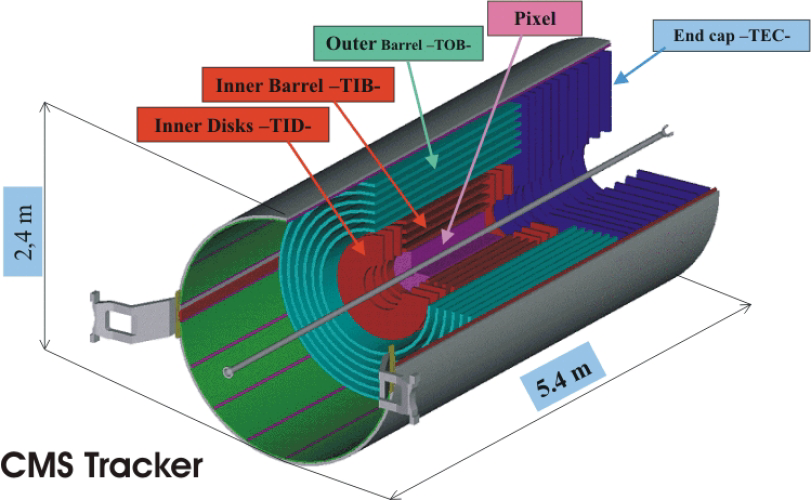
\includegraphics[scale=0.4]{inner_tracker}
  \caption[The inner tracker]{The inner tracker. Pixel and Strip detectors are shown. }
  \label{inner_tracker}
\end{figure}


The outer part of the inner tracker is the strip tracker. It contains several subsystems and is made of almost 9.3 million strips arranged in different configurations in 15148 modules. The first subsystem is the tracker inner barrel (TIB), which consists of the four barrel layers of strip modules. The second subsystem is the tracker inner disks (TIDs), which is made of three disks of strip modules. Increasing the radius to about 60 cm, the tracker outer barrel (TOB) starts. TOB is made of six layers of strips. Finally, to cover high $\eta$ regions, the tracker endcaps (TECs) are used, which are made of two sets of nine disks of strips. 

Each strip is about O(20) cm long. Its thickness varies from 320 $\mu$m  for TIB and TID, to 320 $\mu$m - 500 $\mu$m  for TOB and TEC, respectively. Also width changes from 80 $\mu$m - 141 $\mu$m for TIB and TID, to 97 $\mu$m - 184 $\mu$m  for TOB and TEC, correspondingly. The resolution on the single point in the radial direction is 20 - 50 $\mu$m, and in the z direction it varries from 200 to 500 $\mu$m, depending on the value of r. 

All subsystems of the inner tracker have to be cooled down to about - 20$^{\circ}$.  This requirement is needed to minimise the damage of the tracker caused by the radiation from the collisions and to reduce overheating of the electronics. 

The material of the inner tracker has 0.4 to 1.8 radiation lengths (X$_0$), which corresponds to 0.1 to 0.5 nuclear interaction lengths ($\lambda_i $ ). Numbers vary with the $\eta$.



%%%%%%%%%%%%%%%%%%%%%%%%%%%%%%%%%%%%%%%%%%%%%%%%%


\subsection{The ECAL}


The inner tracker and the ECAL provide the detector with complementary measurements. The tracker focuses on the direction and the momentum of the particle and identifies only charged particles. The ECAL  \cite{ECAL_attendum} (see Fig. \ref{ecal2}), on the other hand, determines the energy of the particles and detects all particles that interact electro-magnetically, including photons and neutral pions. However, primarily the ECAL is designed to measure precisely the energy of electrons and photons. 

The ECAL is a highly granular detector that relies on the lead tungstate crystal (PbWO$_4$) technology. Electrons and photon passing through the crystal interact with its material and their energy is converted into the produced electromagnetic "shower". PbWO$_4$ crystals are known for being a popular choice of the scintillators: interactions with the crystal material produce the scintillation light that is further read out by the electronics. The PbWO$_4$ crystals have a high density (8.28g/cm$^3$), a small radiation length (X$_0 = 0.89$ cm), a short Moliere radius (R = 2.2 cm), and a fast response (80$\%$ of its scintillation light is produced within 25 ns). These characteristics are making PbWO$_4$ crystals ideal candidates for the ECAl, since they guarantee an excellent containment of the electromagnetic shower within the crystals. 

\begin{figure}[H]
  \centering
  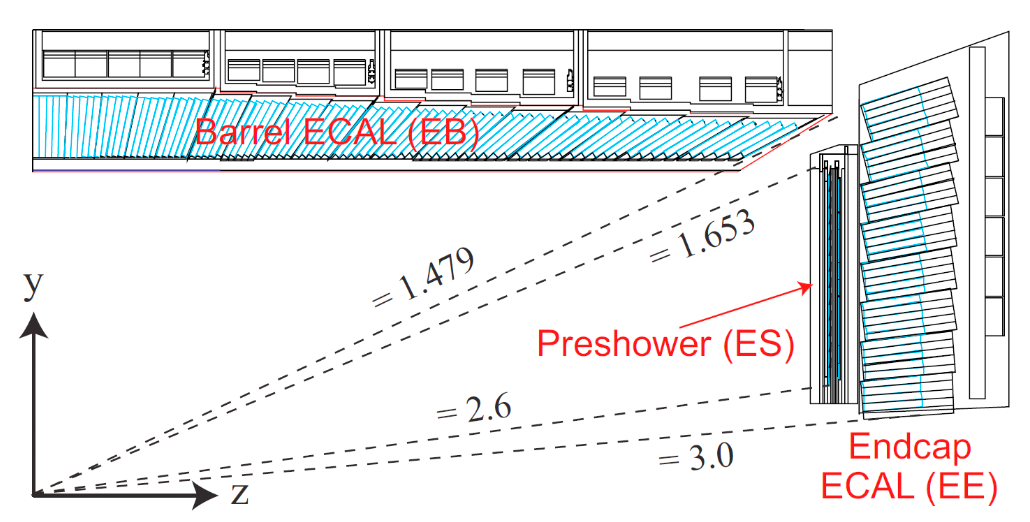
\includegraphics[scale=0.35]{ecal2}
  \caption[The ECAL]{The ECAL and the Preshower detectors.}
  \label{ecal2}
\end{figure}

The ECAL has a barrel part (EB), covering the $|\eta|< 1.479$, and two endcaps (EE) covering 1.479 $< |\eta |  < 3.0$.
In the barrel ECAL is made of 61 200 crystals. Each crystal is 22 by 22 mm with a length of 23 cm. In the endcaps ECAL has 7324 crystals. There each crystal is 28.62 by 28.62 mm with a length of 22 cm. The crystals' layout is following a quasi-geometric projection with axes of crystals slightly tilted to ensure particle trajectories are never aligned with the intercrystal cracks. This layout is optimised for the best particle shower containment with respect to the position of the interaction point.  


The resolution of the ECAL is a function of energy of the incident particle E and can be decomposed into three terms. The first term is a stochastic term that is inversely proportional to the square root of the number N of scintillation photons produced in the interaction. In the main formula N is replaced by E, since N is proportional to E. The second term is a "noise" term that describes the noise in the detector.  The third term is related to detector imperfections and is represented by a constant C. The final dependence of the ECAL energy resolution $\sigma$ on the particle energy E is given by:

  
\begin{equation}
  \left(\frac{\sigma}{E}\right)^2 = \left(\frac{S}{\sqrt{E}}\right)^2 +
  \left(\frac{N}{E}\right)^2 + C^2
  \label{eq:ecal}
\end{equation}

From the dedicated calibration studies, the parameters in the formula above are found to be equal to: S = 2.8$\%$, N = 12$\%$, and C = 0.3$\%$. As a "standard" procedure, the CMS often optimises the performance of the subdetectors for 45 GeV electrons, since they correspond to a classical Drell-Yan decay of Z boson to two electrons. In this case, a typical energy resolution for 45 GeV electrons is about 2$\%$ in EB and 2-5$\%$ for EE. Near the Z peak (91 GeV), the constant terms dominates the resolution.


The ECAL is operated at a temperature of 18 $^{\circ}$ C and the "active width" of the ECAL material corresponds to 25 X$_0$. 

An additional subdetector, called the "Preshower", is installed right in front of the EE and covers 1.653 $ < | \eta |  < $ 2.6. The Preshower is designed to improve the discrimination of single photons from diphoton decays of neutral pions $\pi^0 \rightarrow \gamma \gamma$. This is a sampling calorimeter in which the material that produces the particle shower is distinct from the material that measures the deposited energy. Typically the two materials alternate. 
The Preshower has two lead layers which launch the electromagnetic showers. This "samples" the energy of the particles traversing the Preshower material.  After these layers, 2 mm-wide silicon strips are placed. They measure the deposited energy and transverse profile of the shower shape initiated by the lead layers. The "thickness" of the Preshower material corresponds to 3 X$_0$.

%%%%%%%%%%%%%%%%%%%%%%%%%%%%%%%%%%%%%%%%%%%%%%%%%


\subsection{The HCAL}

Hadrons normally go through the ECAL layers without being stopped. To absorb these particles, the HCAL \cite{HCAL_TDR} (see Fig. \ref{hcal2}) is placed around the ECAL. The HCAL focuses on particles that hadronise. This is a process of the formation of hadrons out of quarks and gluons. The HCAL detects with the charged and neutral hadrons such as pions, kaons, protons, and neutrons. Hadrons also produce collimated streams of secondary particles (jets) and these jets are identified by the HCAL. Additionally, the HCAL is used to measure indirectly the transverse energy of neutrinos, by the momentum imbalance technique, which will be discussed later in this chapter. 

The HCAL is split into HCAL barrel (HB) and HCAL endcap (HE) sections. They cover $ |\eta| < $1.3 and 1.3 $< |\eta| < $3.0 respectively. HB and HE are sampling calorimeters. They are made of a brass absorber and of active plastic scintillating tiles. The brass plates in HB have thickness of 56.5 mm and in HE the thickness if increased to 79 mm. The absorber material corresponds to 5.82 $\lambda_I$ at $\eta = 0$ to almost 10 $\lambda_I$ at $|\eta| < 1.3$.

The gaps in the absorber of the HCAL are filled with an active medium of 70000 plastic scintillator tiles. The scintillation light is guided by wavelength shifting fibres (WLSs) to hybrid photodiodes (HPDs). The scintillator is quite fast with the 68 $\%$ of the light been collected within 25 ns.

\begin{figure}[H]
  \centering
  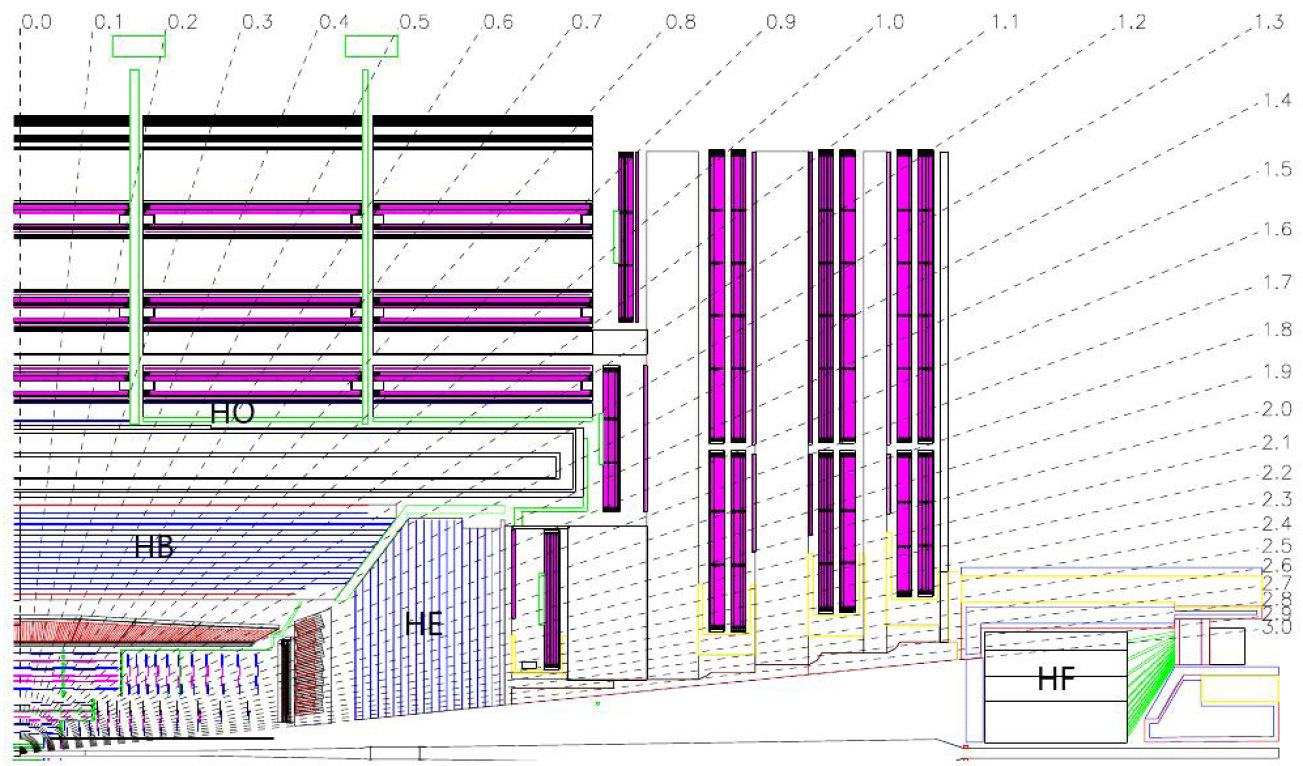
\includegraphics[scale=0.3]{hcal2}
  \caption[The HCAL]{The HCAL with the $\eta$ coverage map.}
  \label{hcal2}
\end{figure}


The CMS also has an outer calorimeter (HO) placed above the HB outside the solenoid. HO is called a tail catcher system and increases the total calorimeter thickness to 11.8 $\lambda_I$ in the barrel, with the magnet coil working as an extra absorption layer. The HO consists of five rings of scintillator tiles. A supplementary iron plate of 19.5 cm in thickness and a second layer of sensitive material are placed around $\eta =$ 0 to enhance the absorber depth there. 

In the forward directions, two forward calorimeters (HF) extend the coverage to  $|\eta| = 5.2$. The HF is composed of steel absorbers and quartz fibres that produce Cherenkov light when the particle in the material travels faster than the light in that medium. The light is further collected by photomultiplier tubes (PMTs). 


Since the HCAL is located between the ECAL and the internal surface of the solenoid, the space allocated for the HCAL is not enough for the HCAL to fully absorb the hadronic showers and this imperfect containment of the hadronic shower limits the performance of the HCAL. Comparing with the formula \ref{eq:ecal}, for the single pions the values are given by:  by S = 115 $\%$, N = 52  $\%$, and C = 5.5 $\%$ \cite{Baiatian_hcal}.


%%%%%%%%%%%%%%%%%%%%%%%%%%%%%%%%%%%%%%%%%%%%%%%%%



\subsection{The Superconding Solenoid}


The NbTi superconducting solenoid (see Fig. \ref{solenoid}) of 6 m in diameter is the core of the CMS experiment. The magnet operates at a temperature of 4.5K. The bulk of the CMS detector weight (90 $\%$) comes from the magnet steel return yoke and structural supports which together weigh 12500 tonnes.
 
 \begin{figure}[H]
  \centering
  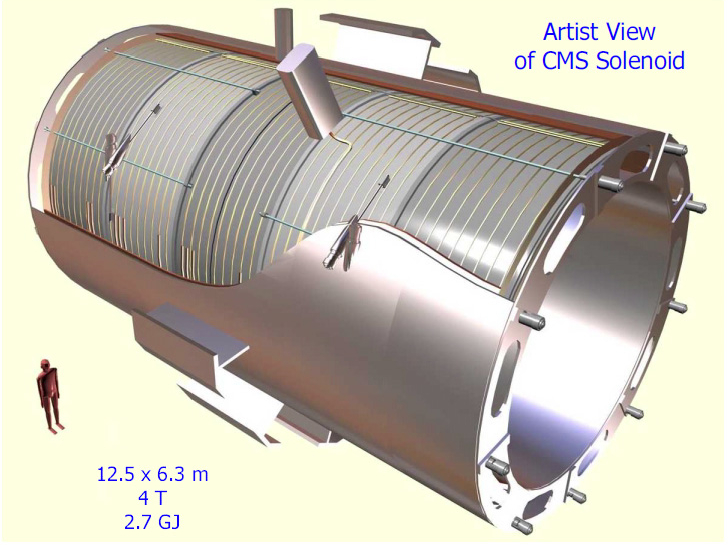
\includegraphics[scale=0.4]{solenoid}
  \caption[The CMS superconducting solenoid]{The CMS superconducting solenoid. The person on the left is shown to emphasise the size of the magnet.}
  \label{solenoid}
\end{figure}

The solenoid is central part in the CMS detector design. The idea was to have a uniform magnetic field capable of bending the trajectories of charged particles as they traverse the detector. When a low energy particle is produced, it has a helical path and will be fully contained within the detector. On the other hand, when a highly energised particle is produced, the trajectory is seen as a "straight" incomplete arc. Both situations lead to imperfect measurement of the momentum. The primary measurements of the tracking system are presumed to be Gaussian distributed; but the momentum of the particle that the tracker measures is not Gaussian distributed. However, the sagitta is Gaussian distributed, and that is why widely used in the particle physics. 

When the particle in the magnetic field passes thorough the material of the detector, the path deviates from the ideal circular line due to random fluctuations and multiple scattering. The sagitta term is used to quantify the depth of the circular arc and is equal to the distance from the centre of the arc to the centre of its base. Since the sagitta is following a Gaussian distribution, it may be approximated by simpler expressions in many calculations of the momentum resolution. 

The magnetic field strength B and the length of the track L are dictated by the design of the detector. Since the momentum resolution is given by $\sigma_p / p^2 \approx \sigma_x / B L^2 $ (see \cite {Hauptman:2011zza}) and improves linearly with magnetic field B, this is the reason why the CMS decided to invest much of the detector space and budget in the magnet. For a track of the length of O(1) m in the magnetic field of O(3) T, the sagitta is equal to 1 mm, which can be measured very precisely. 


%%%%%%%%%%%%%%%%%%%%%%%%%%%%%%%%%%%%%%%%%%%%%%%%%

\subsection{The Muon Tracker}

Many physics analyses in the CMS rely on a precise measurements of the muons in the detector. Although muons are detected by the inner tracker, that information cannot be used by the trigger (will be discussed in the following subsection). Therefore, CMS has an outer tracker or muon tracker \cite{Muon_system_TDR} (see Fig. \ref{cms_muon_system}) located outside the calorimeters and the solenoid. Because of the typical muon energies, muons produced in collisions at the LHC traverse the detector material with the minimal energy losses. To measure energy of muons, the CMS uses the muon tracker, which relies on various gaseous detector technologies. The muon tracker is inserted into the gaps of the flux-return yoke. Tracks in the muon system are used to reconstruct standalone muons, and in combination with the inner tracker, to reconstruct the global muons.

 \begin{figure}[H]
  \centering
  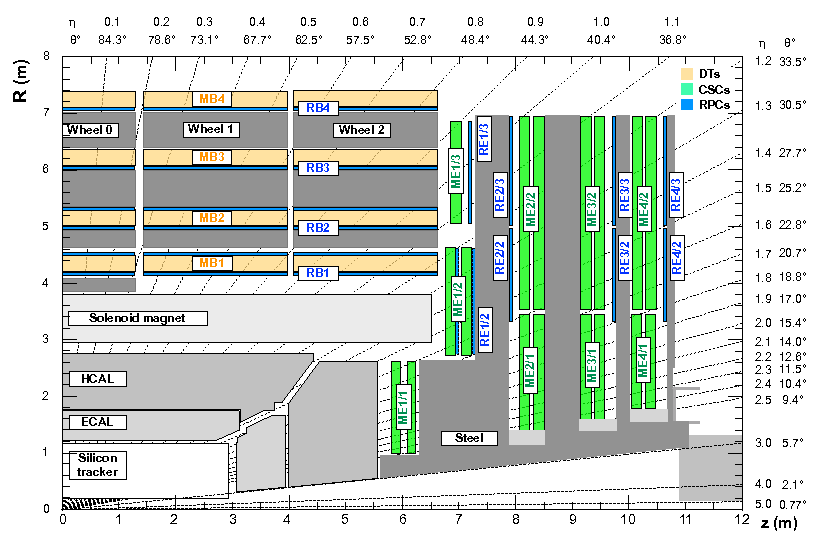
\includegraphics[scale=0.45]{cms_muon_system}
  \caption[The CMS muon tracker]{The CMS muon tracker. DT, CSC, and RPC detectors are shown in yellow, green, and blue respectively.}
  \label{cms_muon_system}
\end{figure}

CMS muon system has three subdetectors: the drift tubes (DTs), the cathode strip chambers detectors (CSCs), and the resistive plate chambers (RPCs). In the barrel region, the CMS is equipped with the DT system, which is 250 drift tubes  arranged into five barrel section ("wheels"). Each wheel is made of four concentric rings of DT stations. The working elements of the DT system - cylindrical cells with the rectangular base of 4.2 by 1.3 cm$^2$ - are tubes with an anode wire in the the mix of argon and CO$_2$ gases. DT cells are 2.4 m long and are organised in three groups of four elements (three "super-layers"). When the muon passes through super-layers, it ionises the gas in the cells and released electrons start moving to anodes. Using the time it takes for electrons to reach the anodes, the muon position and direction can be determined. DT resolution of a single-cell hit positions ranges from 200 $\mu$m in the r-$\varphi$ plane to 200-600 $\mu$m for forward directions. 

CSCs are used in the forward direction to cover the region of 0.9 $ <|\eta|<$2.4. CSCs chambers are multi-wire chambers made of cells  that have a trapezoidal shape. Chambers contain radial copper cathode strips and, perpendicular to those, gold-plated tungsten anode wires. Each cell is filled with the mix of Argon, CO$_2$, and CF$_4$ gases. The strip cells have a single-layer resolution of 300-900 $\mu$m. A CSC chamber provides a spatial resolution of 40 -150 $\mu$m.


To improve the performance of DTs and CSCs, RPCs are used and are covering the barrel and endcaps in the range of $|\eta| <$ 1.9. 
RPCs are double-gap chambers consisting of two resistive 2 mm in thickness Bakelite layers separated by a 2 mm layers filled with a mix of C$_2$H$_2$F$_4$, $i$C$_4$H$_{10}$, and SF$_6$ gases.

RPCs operate in avalanche mode, producing an avalanche when the muon traverses the gas of the cell. RPCs have a spatial resolution of 0.8 - 1.2 cm, which is not as good as the ones provided by other muon subsystems, but RPCs have an advantage in terms of an excellent time resolution - just 3 ns. The barrel and the endcaps contain in total 10 RPC stations.



%%%%%%%%%%%%%%%%%%%%%%%%%%%%%%%%%%%%%%%%%%%%%%%%%%%%%%%%%%%%

\subsection{The Triggers and DAQ}

The CMS trigger \cite{Trigger} is a system responsible for selecting events of interest and storing them for the offline analysis. The trigger has two stages: the L1 trigger (see Fig. \ref{L1trigger}), which reduces the event rate from 40 MHz to 100 kHz, and the HLT trigger, which further decreases the rate to nearly 1 kHz. The L1 trigger consists of the custom hardware that processes a part of the information from calorimeters and outer tracker systems. The HLT trigger is a part of the detector readout system (DRS) and uses the full detector information for event reconstruction. The HLT is a computing farm consisting of 22000 CPU cores that produce a decision on whether to save or to skip the event in an average time of about 220 $\mu$s. DRS is integrated in the higher level data acquisition (DAQ) system \cite{DAQ}. The selected events are collected and sent by the DAQ to the tapes of the CERN Tier-0 for the persistent storage. 


L1 and HLT systems have differences and similarities. They operate at the different time scales and the volumes of data they are processing are completely different. However, the goals of these systems are the same - to identify and reconstruct physics objects and combine their properties to produce an acceptance/rejection decision for each event. 

%%%%%%%%%%%%%%%%%%%%%%%%%%%%%%%%%%%%%%%%%%%%%%%%%


\subsubsection{The L1 Trigger}


L1 system \cite{CMS_TDR} contains a "menu" of 500 algorithms or "seeds" designed to identify useful physics events. These menus include trigger criteria varying from basic single-object identification to complicated selections requiring some topological conditions to be met. Each seed has a set of assigned "Prescale" factors $f$ that reduce the rate of events accepted by a particular trigger algorithm from 100$\%$ to $100/f\%$. Prescale factors are necessary since the luminosity level decreases during the run period. They adjust the trigger rate to keep it constant during the data taking time. 

Since the processing time of the L1 system is very important for the whole CMS operation, the L1 is built using FPGAs and ASICs custom hardware. L1 produces decisions within 3.8 $\mu$s. Data from all the calorimeters is first processed by the L1 regional calorimeter trigger (RCT) and then by a more selective global calorimeter trigger (GCT). 

 \begin{figure}[H]
  \centering
  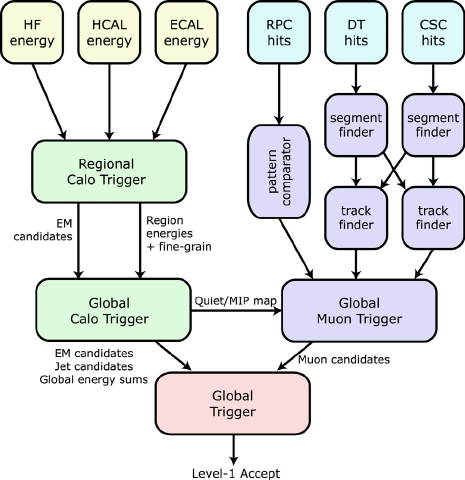
\includegraphics[scale=0.5]{L1trigger}
  \caption[The CMS L1 trigger layout]{The CMS L1 trigger layout.}
  \label{L1trigger}
\end{figure}

The RCT receives the information about energy deposits from all calorimeters and covers the range $|\eta|<$5. The RCT processes this information in parallel and produces e/$\gamma$ candidates as an output. The information from the inner tracker is not available, therefore, L1 identifies both electrons or photons, but cannot distinguish them. L1 also detects jets, taus, missing transverse energy (MET or \ETslash or \PTslash), and muons. L1 RCT is responsible for determining the first estimates of the several main parameters of interest: $p_T$, isolation (described later in this chapter), etc. 

First stage reconstruction uses particle "hits" in the muon detectors and analyses them using track finder algorithms. All three muon detectors of the CMS are used by the L1 muon trigger. Using DT and CSC systems, track segments from the hit information are identified. The pattern recognition algorithms are applied to these segments to reconstruct muon candidates and measure their momenta. 

More complex but slower algorithms then re-use hits for a more precise particle identification using a global muon trigger (GMT). 
The hits from the RPCs are used directly by the pattern comparator trigger (PACT) that reconstructs muon candidates at the high radii. Then several regional track finder algorithms sort the identified muon candidates and send this information to the GMT. Each candidate contains $p_T$ and angular information. 

The GMT then combines the muon information from different subsystems to avoid duplicating the candidates. The GMT also performs more tight track quality checks and may discard a portion of the input candidates it received. 

Finally, the information from the GCT and GMT is combined by a global trigger (GT). The GCT sorts the created e/$\gamma$ candidates, identifies jets, and calculates \ETslash. The final decision of the GT is to store or to skip the event. If the event satisfies the acceptance requirements and is going to be kept, the L1 accept signal (LAS) is generated and propagated by the trigger control and distribution system (TCDS) to all subdetectors. 


The GT is the final step of the CMS L1 trigger system and implements a menu of triggers. The output of this system is used as an input to the HLT algorithms. 

%%%%%%%%%%%%%%%%%%%%%%%%%%%%%%%%%%%%%%%%%%%%%%%%%


\subsubsection{The HLT Trigger}

The selection done by the HLT mimics the offline analysis - for all reconstructed objects in the event: electrons, muons, and jets - the identification criteria is applied to select only events of interest. What these events are each offline analysis defines in a different way, but to name a few, almost all analyses need true prompt leptons, well reconstructed jets, or some other commonly used objects. 


The HLT computing farm has the event filter farm, which consists of filter-builder units (FBU). In the FBU the parts of the events and information from different detector subsystems is combined to produce "complete" events. Then the filter unit unfolds the raw detector data into experiment specific data structure and performs the event reconstruction and trigger filtering. 


The whole event processing procedure of the HLT is centered around the HLT path. The HLT path is a set of algorithmic instructions that in a sequential manner reconstructs physics objects and performs the object selection. The complexity of the steps in the path sequence increases and the quality of the physics objects (the probability to have a correct label) improves too. After this step is completed, selected events are sent to another software processing farm. In this storage manager farm, the date is archived, stored locally on disk, and later sent to the CMS Tier-0 computing center for offline use. 

Most data enters the queue for processing and is ready to be sent to Tier-0 very soon. In some cases the special data, the "parked" data, may be collected and kept until the run is finished. In this situations the CMS tape is used and the data has a high-priority for "parking". This may include "hot topic" analyses such as vector boson fusion or parton distribution studies such as Drell-Yan process.

The output of the HLT is limited by capacities of the Tier-0. This includes the bandwidth of the data transfer as well as the amount of available tape. This complicates the work of the DAQ, since in addition to physics data streams, the calibration streams also need to be stored. These streams, though, use information only from few subdetectors. 


%%%%%%%%%%%%%%%%%%%%%%%%%%%%%%%%%%%%%%%%%%%%%%%%%

\subsubsection{The DAQ system}



The DAQ systems in the modern high energy physics are responsible for any tasks. The challenges are well known: high data rates and volumes, limited tape space and transfer bandwidth. CMS DAQ is based on the homogeneous architecture, scales well with the different beam energy regimes and data rates, and stable  performance  in  a  variety  of  operating  conditions.  

To illustrate an example of a complex computing task that is elegantly solved by the DAQ system, let us discuss in more details the aforementioned FBUs system of the HLT. FBU relies on a single multi-core machine and the communications with other units are done via shared memory. The data from the full detector is used for the filtering process. Complicated offline-like reconstruction algorithms are then used for the full precision event selection. With more CPU cores available for the Run-2, the per-event time budget is increased to "comfortable" 175 ms per event, which is a long enough time to run most of the CMS reconstruction algorithms. 

The current CMS DAQ was developed to address these core requirements: 

\begin{itemize}
\item The data from one or several data transfer lines is available for other lines,
\item the event building is done in parallel profiting from multiple processing units,
\item almost real-time process monitoring,
\end{itemize}


Proper design patterns are used in the software for DAQ, which decouple the user  interface from the implementation. The design also allows for the remote control. The  software  system  can be run on a number of different  operating  systems  and  hardware  platforms.   The memory  management  tools  of  the  underlying  system  are not linked directly to the applications, it is done using a dedicated abstract addressing  scheme.

%%%%%%%%%%%%%%%%%%%%%%%%%%%%%%%%%%%%%%%%%%%%%%%%%
  
\subsection{The CMS design}

Now that we discussed all CMS subdetectors and DAQ, we can look back and summarise in one list what were the requirements on the design of the CMS detector to successfully complete its physics program. Here we refer to the CMS Technical Design Report \cite{CMS_TDR}: 


\begin{itemize}
\item good muon momentum resolution over the momentum scale covering almost a TeV range, good dimuon resolution (mostly $Z \rightarrow \mu \mu$ and $H \rightarrow \mu \mu$) at the O(100) GeV. The capability to determine correctly the charge of the highly energetic muon all the way up to 1 TeV,
\item good momentum resolution of all charged particles in the inner tracker,
\item good diphoton mass resolution with the focus on the $H \rightarrow \gamma \gamma$ discovery channel. Also, the ability to reject $\pi^0 \rightarrow \gamma \gamma$, which is one of the main background processes to many physics analyses.  This requirement mostly concern the performance of the ECAL,
\item good resolution of the missing transverse energy (discussed in the section below) and of the mass of the two-jet system. This task depends heavily on the performance of the HCAL.
\end{itemize}

In the next chapter we will dive deep into the physics analysis of the data produced by the LHC and collected with the CMS detector that has been used to perform the measurement of the double Higgs boson decays.
%%%%%%%%%%%%%%%%%%%%%%%%%%%%%%%%%%%%%%%%%%%%%%%%%


\section{The object reconstruction}\label{sec:cms_reconstruction}

  
  - somewhere a section on physics objects where you discuss that there are tracks, there are jets, there are b-jets, what it means an isolated lepton, what it means missing momentum, and so forth. For example, Ekaterina has a section on particle flow, if I remember right, where she discusses that. Or you can have a section that just discuses the proton-proton collisions environment and explains that many particles created in collisions are unstable and decay right away. What is observable in an experiment such as CMS is longer-lived or stable particles. These include electrons, muons, photons, and some ground state hadrons. At the same time, energetic quarks or gluons hadronize and can be seen in a particle detectors as jets of hadrons (so define jets here). Same for tau leptons, we detect them either as electrons/muons, or hadronic jets. Etc. If you have such a conceptual paragraph here, some time later you can have a particle flow discussion when it is time to be more specific. But discussion at this level above would allow you to then discuss the requirements on CMS design using terms like b-jets or isolated leptons.

  EGAMMA AT LEAST SAY THAT HAS BEEN WORKING AND SHOW SOME PLOTS?

%\end{normalsize}       % 28 to 58 -> 31 pages for the chapter (font 12)
\end{small}             % 28 to 56 -> 29 pages for the chapter (font almost 11)
%\end{footnotesize}  % 28 to 51 -> 24 pages for the chapter (font 10)
 
 

\iffalse  % do not forget to end this with "\fi" to have a block invisible for LaTex


%%%%%%%%%%  - start Hbb abbreviations
% Useful aliases
\newcommand\T{\rule{0pt}{2.3ex}}
\newcommand\B{\rule[-1.0ex]{0pt}{0pt}}



\providecommand{\mll}{\ensuremath{\mathrm{m}_{\ell\ell}}\xspace}
%\providecommand{\mll}{\ensuremath{\mathrm{m_{\textit{ll}}}}\xspace}                                                                         \
                                                                                                                                              
%\providecommand{\mll}{\ensuremath{\mathrm{m}_{\Pl\Pl}}\xspace}                                                                              \
                                                                                                                                              
%\providecommand{\mbb}{\ensuremath{\mathrm{m}_{bb}}\xspace}                                                                                   
\providecommand{\mbb}{\ensuremath{\mathrm{m}_{bb}}\xspace}

\newcommand*{\MGMCatNLO}{\textsc{MadGraph5}\_aMC@NLO\xspace} 





\def\Znn      {\ensuremath{\mathrm{Z}(\cPgn\cPgn)}}
\def\ZnnH     {\ensuremath{\mathrm{Z}(\cPgn\cPgn)\mathrm{H}}}
\def\ZnnV     {\ensuremath{\mathrm{Z}(\cPgn\cPgn)\mathrm{V}}}
\def\ZllH     {\ensuremath{\mathrm{Z}(\ell\ell)\mathrm{H}}}
\def\ZllV     {\ensuremath{\mathrm{Z}(\ell\ell)\mathrm{V}}}
\def\ZmmH     {\ensuremath{\mathrm{Z}(\Pgm\Pgm)\mathrm{H}}}
\def\ZeeH     {\ensuremath{\mathrm{Z}(\Pe\Pe)\mathrm{H}}}
\def\Wln      {\ensuremath{\mathrm{W}(\ell\cPgn)}}
\def\WlnH     {\ensuremath{\mathrm{W}(\ell\cPgn)\mathrm{H}}}
\def\WlnV     {\ensuremath{\mathrm{W}(\ell\cPgn)\mathrm{V}}}
\def\WlnHbb   {\ensuremath{\mathrm{W}(\ell\cPgn)\mathrm{H}(\bbbar)}}
\def\WmnH     {\ensuremath{\mathrm{W}(\Pgm\cPgn)\mathrm{H}}}
\def\WenH     {\ensuremath{\mathrm{W}(\Pe\cPgn)\mathrm{H}}}
\def\WtnH     {\ensuremath{\mathrm{W}(\Pgt\cPgn)\mathrm{H}}}
\def\WtoLN    {\ensuremath{\mathrm{W}\to\ell\cPgn}}
\def\WtoEN    {\ensuremath{\mathrm{W}\to\Pe\cPgn}}
\def\WtoMN    {\ensuremath{\mathrm{W}\to\Pgm\cPgn}}
\def\ZtoBB    {\ensuremath{\mathrm{Z}\to\bbbar}}
\def\ZtoNN    {\ensuremath{\mathrm{Z}\to\cPgn\bar{\cPgn}}}
\def\ZtoLL    {\ensuremath{\mathrm{Z}\to\ell\ell}}
%\newcommand\ZtoLL {\ensuremath{\cPZ\to\ell\ell}}
\def\ZtoMM    {\ensuremath{\mathrm{Z}\to\MM}}
\def\ZtoEE    {\ensuremath{\mathrm{Z}\to\EE}}
\def\WmnJ     {\ensuremath{\mathrm{W}(\Pgm\cPgn)\mathrm{+jets}}}
\def\ZmmJ     {\ensuremath{\mathrm{Z}(\Pgm\Pgm)\mathrm{+jets}}}
\def\ZnnJ     {\ensuremath{\mathrm{Z}(\cPgn\bar{\cPgn})\mathrm{+jets}}}
\def\WJ       {\ensuremath{\mathrm{W}+\mathrm{jets}}}
\def\HBB      {\ensuremath{\mathrm{H}\to\bbbar}}
\def\HZZ      {\ensuremath{\mathrm{H}\rightarrow ZZ}}
\def\HTT      {\ensuremath{\mathrm{H}\to\TT}}
\def\mtW      {\ensuremath{M_{\mathrm{T}}}}
\def\mtop     {\ensuremath{M_{\mathrm{t}}}}
\def\pt       {\ensuremath{p_{\mathrm{T}}}}
\def\ptl      {\ensuremath{p_{\mathrm{T}}^{\ell}}}
\def\MyZ      {\ensuremath{\mathrm{Z}}}
\def\MyW      {\ensuremath{\mathrm{W}}}
\def\MyH      {\ensuremath{\mathrm{H}}}
\def\QCD      {\ensuremath{\mathrm{multijet}}}
\def\Vudscg   {\ensuremath{\mathrm{V+udscg}}}
\def\Wudscg   {\ensuremath{\mathrm{W+udscg}}}
\def\Wenudscg {\ensuremath{\mathrm{W}(\Pe\cPgn)+\mathrm{udscg}}}
\def\Wmnudscg {\ensuremath{\mathrm{W}(\Pgm\cPgn)+\mathrm{udscg}}}
\def\Wenbb    {\ensuremath{\mathrm{W}(\Pe\cPgn)+\bbbar}}
\def\Wmnbb    {\ensuremath{\mathrm{W}(\Pgm\cPgn)+\bbbar}}
\def\Wlnbb    {\ensuremath{\mathrm{W}(\ell\cPgn)+\bbbar}}
\def\Zeebb    {\ensuremath{\mathrm{Z}(\Pe\Pe)+\bbbar}}
\def\Zmmbb    {\ensuremath{\mathrm{Z}(\Pgm\Pgm)+\bbbar}}
\def\Zudsg    {\ensuremath{\mathrm{Z+udsg}}}
\def\Zudscg   {\ensuremath{\mathrm{Z+udscg}}}
\def\Zbb      {\ensuremath{\mathrm{Z}+\bbbar}}
\def\Zeeudscg {\ensuremath{\mathrm{Z}(\Pe\Pe)+\mathrm{udscg}}}
\def\Zmmudscg {\ensuremath{\mathrm{Z}(\Pgm\Pgm)+\mathrm{udscg}}}
\def\Zenbb    {\ensuremath{\mathrm{Z}(\Pe\cPgn)+\bbbar}}
\def\Zmnbb    {\ensuremath{\mathrm{Z}(\Pgm\cPgn)+\bbbar}}
\def\Wbb      {\ensuremath{\mathrm{W\bbbar}}}
\def\W0b      {\ensuremath{\mathrm{W0\b}}}
\def\W1b      {\ensuremath{\mathrm{W1\b}}}
\def\W2b      {\ensuremath{\mathrm{W2\b}}}
\def\Z0b      {\ensuremath{\mathrm{Z0\b}}}
\def\Z1b      {\ensuremath{\mathrm{Z1\b}}}
\def\Z2b      {\ensuremath{\mathrm{Z2\b}}}
\def\Zcc      {\ensuremath{\mathrm{Z\ccbar}}}
\def\Vbb      {\ensuremath{\mathrm{V+\bbbar}}}
\def\Zll      {\ensuremath{Z(\ell\ell)}}
\def\Zmm      {\ensuremath{Z(\mu\mu)}}
\def\Zee      {\ensuremath{Z(ee)}}
\def\Mjj      {\ensuremath{M(\mathrm{jj})}}
\def\ptjj     {\ensuremath{{\pt}(\mathrm{jj})}}
\def\MZ       {\ensuremath{M_{\mathrm{Z}}}}
\def\dRJJ     {\ensuremath{\Delta R(\mathrm{jj})}}
\def\dPhiJJ   {\ensuremath{\Delta\varphi(\mathrm{jj})}}
\def\dEtaJJ   {\ensuremath{\Delta\eta(\mathrm{jj})}}
\def\dphiVH   {\ensuremath{\Delta\phi(\mathrm{V,H})}}
\def\dphiWH   {\ensuremath{\Delta\phi(\mathrm{W,H})}}
\def\dphiZH   {\ensuremath{\Delta\phi(\mathrm{Z,H})}}
\def\dphiMJ   {\ensuremath{\Delta\phi(\mathrm{pfMET,J})}}
\def\dphiMtkM {\ensuremath{\Delta\phi(\mathrm{pfMET,trkMET})}}
\def\dPhiMETlep {\ensuremath{\Delta\phi(\mathrm{pfMET,lep})}}
\def\cosTH    {\ensuremath{\cos{\theta^*}}}
\def\dThPull  {\ensuremath{\Delta\theta_{\mathrm{pull}}}}
\def\ptV      {\ensuremath{p_{\mathrm{T}}(\mathrm{V})}}
\def\ptH      {\ensuremath{p_{\mathrm{T}}(\mathrm{H})}}
\def\ptZ      {\ensuremath{p_{\mathrm{T}}(\mathrm{Z})}}
\def\ptW      {\ensuremath{p_{\mathrm{T}}(\mathrm{W})}}
\def\Naj      {\ensuremath{N_{\mathrm{aj}}}}
\def\Nj      {\ensuremath{N_{\mathrm{jets}}}}
\def\Nal      {\ensuremath{N_{\mathrm{al}}}}
\def\AddJetMaxCSV {\ensuremath{\mathrm{max}\mathrm{CSV}_{\mathrm{aj}}}}
\def\AddJetMaxCMVA {\ensuremath{\mathrm{max}\mathrm{CMVA}_{\mathrm{aj}}}}
\def\AddJetMindR  {\ensuremath{\mathrm{min}\Delta R(\mathrm{H,aj})}}
\def\etaTF    {\ensuremath{\left | \eta \right | < 2.5}}
\def\Bexp     {\ensuremath{B_{\mathrm{exp}}}}
\def\Bobs     {\ensuremath{B_{\mathrm{obs}}}}
\def\Nobs     {\ensuremath{N_{\mathrm{obs}}}}
\def\lumi15     {\ensuremath{2.32\fbinv}~}
%\def\lumi16     {\ensuremath{22.02\fbinv}~}
\def\lumi16     {\ensuremath{12.9\fbinv}~}
\def\lumiEight     {\ensuremath{18.9\fbinv}~}
\def\lumiSeven     {\ensuremath{5.0\fbinv}~}
\def\ppWZ {\ensuremath{\sigma(pp \rightarrow WZ)}}
\def\ppZZ {\ensuremath{\sigma(pp \rightarrow ZZ)}}
\def\muBDT {\ensuremath{\mu = 1.09 {}_{-0.21}^{+0.24}}}
\def\muMbb {\ensuremath{\mu = 0.97 {}_{-0.29}^{+0.32}}}
\def\muWZ {\ensuremath{\mu_{\mathrm{WZ}} = 1.37 {}_{-0.37}^{+0.42}}}
\def\muZZ {\ensuremath{\mu_{\mathrm{ZZ}} = 0.85 {}_{-0.31}^{+0.34}}}
\def\XSZZ {\ensuremath{\sigma (pp \to \mathrm{ZZ}) = 6.5 \pm 1.7(\mathrm{stat.}) \pm 1.0 (\mathrm{syst.}) \pm 0.9 (\mathrm{theo.}) \pm 0.2 (\mathrm{lumi.})\, \rm{pb}}}
\def\XSWZ {\ensuremath{\sigma (pp \to \mathrm{WZ}) = 30.7 \pm 9.3(\mathrm{stat.}) \pm 7.1 (\mathrm{syst.}) \pm 4.1 (\mathrm{theo.}) \pm 1.0 (\mathrm{lumi.})\, \rm{pb}}}
\def\XSZZfid {\ensuremath{\sigma (pp \to \mathrm{ZZ}) = 0.90 \pm 0.23(\mathrm{stat.}) \pm 0.16 (\mathrm{syst.})\, (\mathrm{syst.})\, \rm{pb}}}
\def\XSWZfid {\ensuremath{\sigma (pp \to \mathrm{WZ}) = 4.79 \pm 1.41(\mathrm{stat.}) \pm 1.12 (\mathrm{syst.})\, \rm{pb}}}
\def\theoryXSWZ {\ensuremath{\ppWZ = 22.3 \pm 1.1\, \rm{pb}}}
\def\theoryXSZZ {\ensuremath{\ppZZ = 7.7 \pm 0.4\, \rm{pb}}}
\def\theoryXSWZfid {\ensuremath{\ppWZ = 3.39 \pm 0.17\, \rm{pb}}}
\def\theoryXSZZfid {\ensuremath{\ppZZ = 1.03 \pm 0.05\, \rm{pb}}}

% for taus
\def\mtau       {\ensuremath{\tau}\xspace}
\def\dyjets {\ensuremath{DY+\mathtt{jets}}\xspace}
\def\Wtnudscg {\ensuremath{\mathrm{W}(\mtau\cPgn)+\mathrm{udscg}}}
\def\Wtnbb    {\ensuremath{\mathrm{W}(\mtau\cPgn)+\bbbar}}

\def\minMETMHT      {\ensuremath{\mathrm{min(MET,MHT)}}}
\def\MHT      {\ensuremath{\mathrm{MHT}}}
\def\antiQCDtight      {\ensuremath{\mathrm{anti\mbox{-}QCD_{tight}}}}
\def\antiQCDloose      {\ensuremath{\mathrm{anti\mbox{-}QCD_{loose}}}}
\def\ChHEF1      {\ensuremath{\mathrm{CHF1}}}
\def\CSVmax      {\ensuremath{\mathrm{CSV_{max}}}}
\def\CSVmin      {\ensuremath{\mathrm{CSV_{min}}}}
\def\CMVAmax      {\ensuremath{\mathrm{CMVA_{max}}}}
\def\CMVAmin      {\ensuremath{\mathrm{CMVA_{min}}}}
\def\softActivity {\ensuremath{\mathrm{soft-activity}}}


\newcommand\PQb   {\ensuremath{b}}



%
% copied from PAS
\def\VH       {\ensuremath{\mathrm {VH}}}
\def\mH       {\ensuremath{m_\PH}}
%\def\mH{\ensuremath{\mathrm{m_H}}}
\def\VtoBB    {\ensuremath{\mathrm{V}\to\bbbar}}

\newcommand\Voneb   {\ensuremath{\Vvar+\cPqb}}
\newcommand{\Vvar}{\ensuremath{\cmsSymbolFace{V}}\xspace}
\newcommand\Vtwob   {\ensuremath{\Vvar+\bbbar}}

%%%%%%%%%%  - end Hbb abbreviations





\chapter{Analysis overview}
\label{ch:an_overview}

In 2012, CMS~\cite{HiggsCMS} and
ATLAS~\cite{HiggsAtlas} collaborations officially discovered a Higgs-like particle and with that breakthrough the picture of the
SM \cite{Salam:1961en,Glashow:1961tr,Weinberg:1967tq}
of the particle physics has been completed. 
Most of the basic properties of the Higgs
boson have been measured. 
However, it remains difficult to distinguish several processes with very low
cross sections from the
irreducible SM background processes with a similar signature. 
One such important but rare process is a double Higgs (HH) boson
production. HH directly relates to the Higgs boson self-coupling, and thus,  
has an access to the shape of the Higgs boson potential. In the SM, HH
production is a non-resonant process with a cross section of $\sigma$
=  fb~\cite{HHXsec} at $\sqrt{s}=13$~TeV. 

Several Beyond the Standard
Model (BSM) theories and models, such as supersymmetry, composite Higgs, Warped Extra Dimensions (WED)~\cite{Dolan:2012ac, Huang:2017nnw, Kanemura:2016tan, Oliveira:2014kla, WED}, predict scenarios when the double Higgs boson
cross section is significantly increased and may be observed with the current data.
There may be two different types of the BSM HH production: a non-resonant production,
introducing BSM terms to the SM lagrangian or a resonant production,
in which the process is mediated by a narrow width heavy mass resonance that subsequently would decay to SM Higgs bosons. 
~\cite{WED}. %%\newline
\vspace{1em} % adds some space


In this analysis through the gluon fusion mechanism a heavy narrow
resonance, such as RS1 KK graviton or RS1 radion ("graviton" or "radion" later in the text) \cite{BG1,BG2,BG3} is produced. It decays to two Higgs bosons, which further decay to the bb pair (the first Higgs boson) and the ZZ/WW pair (the other Higgs boson). 
The analysis covers masses of graviton/radion from 250 GeV to 1000 GeV. Since no evidence of the signal has been reported by the previous HH analyses, we proceed directly to setting 95 \% upper confidence
limits on the production of the graviton with a subsequent
decay to Higgs bosons times the branching ratios of the Higgs
boson decaying to a pair of b quarks and the other Higgs boson to two
leptons and two neutrinos respectively (Fig. ~\ref{fig:BGtoHH}). We observe no deviation with the given data and
evaluated uncertainties, the results are compatible with the Standard
Model.


\begin{figure}[!htb]%hbpt?
  \begin{center}
    %\raisebox{0.17\height}
    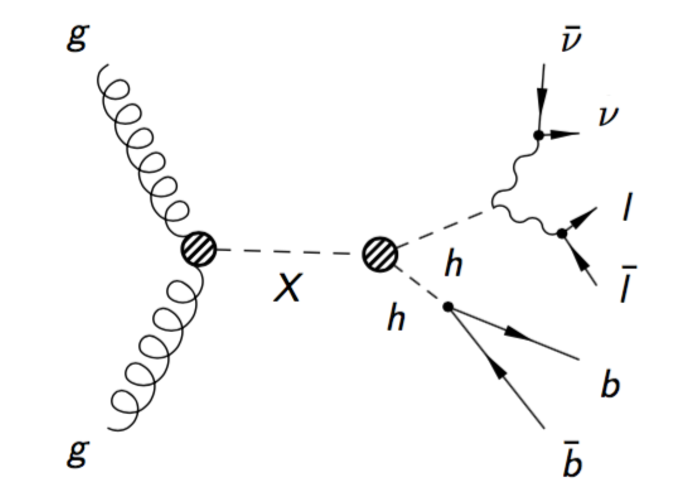
\includegraphics[width=0.45\textwidth]{BGtoHH.pdf}
    \caption{ The Feynman diagram of the graviton/radion production with the subsequent decay to HH. HH system decays to a pair of b quarks and Z bosons. Shown is 2 b quarks, 2 leptons, and 2 neutrinos final state.
    }
    \label{fig:BGtoHH}
  \end{center}
\end{figure}


\section{Analysis Strategy}

The analysis is based on ntuples and object selection from the approved VHbb sister analysis~\cite{VHbb_inspire}. Leptons, b jets, and the missing transverse energy (MET) are reconstructed using the standard CMS procedures~\cite{CMSreco} and the Particle Flow (PF) algorithm~\cite{PFalgo}. b-jets are identified using the Combined MVA v2 (CMVA) algorithm~\cite{BTagtwiki}. Then, on shell Z boson candidates are selected of dilepton pairs of the same flavour with a net charge zero for a pair. Higgs boson candidate decaying to b quarks (Hbb) is reconstructed as a pair of b jets with the highest CMVA output value. Finally, double Higgs boson pseudo-transverse mass, which is used in the shape analysis to extract limits, is constructed computing the transverse mass of the sum of the Lorentz vectors of the two leptons forming the on-shell Z, MET, and a pair of the b jets forming the \HBB. Additionally, a cut on the missing transverse energy is introduced to preserves the orthogonality with the existing HIG-18-013 ``2b 2l 2q'' analysis, which also works with the $bbZZ$ decays. In a similar fashion, the cut on the Z mass ($m_Z > 76$ GeV) is used to orthogonalise the analysis with respect to the HH phase space used in the legacy $bbWW$ analysis where the final signature is identical to ours. Lastly, the cut on the BDT is used to reduce the background contamination in the signal region.

Main backgrounds are \ttbar and Drell-Yan in association with jets. To determine their normalization, we construct two dedicated control region, which are correspondingly \ttbar and Drell-Yan dominated. Then, during the the simultaneous fit of signal region (SR), as well as control region \ttbar (CRTT), and control region Drell-Yan (CRDY), we obtain rates for these processes. Others, minor backgrounds, are single top production, diboson samples (WW, WZ, ZZ), and ZH production and are determined from the Monte Carlo (MC) simulation. 
%We assign systematics uncertainties on the QCD scale corresponding to each process. Also uncertainty associated with the imperfect knowledge of the single top cross section is added.

In the next chapters we will discuss all of the aspects of the analysis in details starting with the chapter on Data. 
 \clearpage




\subsection{Data}
This measurement uses the full dataset of 2016 collected with the CMS detector in pp collisions
at 13 TeV center-of-mass energy with the corresponding integrated luminocity of 35.9 ~\fbinv. 

As the measurement is based on dilepton signatures, the DoubleMuon and DoubleElectron primary
datasets are analyzed and only on-shell \Zll~decays are considered, where $\ell=\Pe, \Pgm$.
 
The run periods and the corresponding integrated luminosities are listed in Table ~\ref{tab:datasets} for DoubleMuon channel, DoubleElectron channel numbers are similar.
\begin{table}[htbp]
\caption{List of used 2016 DoubleMuon data sets.
%\lumi16  across all modes.  
An uncertainty of $2.5\%$ is  assigned for the 2016 data set luminosity~\cite{lumiUnc}}

\label{tab:datasets}
\begin{center}
\scalebox{0.9}{
\begin{tabular}{|c|c|} \hline%\hline
Dataset       & $\int\cal L$ (\fbinv) \\
\hline
%{\tt DoubleMuon\_Run2016B-03Feb2017-v1}       & \multirow{2}{*}{$\sim$5.9}  \\
{\tt DoubleMuon\_Run2016B-03Feb2017-v2}       & {$\sim$5.9}  \\
%{\tt DoubleMuon\_Run2016B-03Feb2017-v2}       &   \\
{\tt DoubleMuon\_Run2016C-03Feb2017-v1}       & $\sim$2.7 \\
{\tt DoubleMuon\_Run2016D-03Feb2017-v1}       & $\sim$4.3 \\
{\tt DoubleMuon\_Run2016E-03Feb2017-v1}       & $\sim$4.1 \\
{\tt DoubleMuon\_Run2016F-03Feb2017-v1}       & $\sim$3.2 \\
{\tt DoubleMuon\_Run2016G-03Feb2017-v1}       & $\sim$3.8 \\
{\tt DoubleMuon\_Run2016H-03Feb2017-v1}       & $\sim$11.8 \\
\hline
Total Lumi                        & 35.9 \\
\hline%\hline
\end{tabular}
}
\end{center}
\end{table}

\subsection{Triggers\label{sec:triggers}}
%% Because the analysis is performed in the dielectron and dimuon channels, unprescaled dilepton 
%% triggers with the lowest available transverse momentum thresholds are utilized. The triggers at the L1 and
%% HLT level are listed in table ~\\ref{tab:trgs2015}. Dielectron trigger requires the leading electron to pass $23$ GeV $p_{T}$ cut and $12$ GeV $p_{T}$ cut for the subleading electron. Offline cuts are $25$ GeV $p_{T}$ cut and $15$ GeV $p_{T}$ cut correspondinly. Dimuon triggers require the leading muon to pass $17$ GeV $p_{T}$ cut and $8$ GeV $p_{T}$ cut for the subleading muon with the $20$ GeV $p_{T}$ cut and $15$ GeV $p_{T}$ cut for offline selection correspondinly. $\eta$ region in the gap is excluded (1.4442 to 1.566). 

Because the analysis is performed in the dielectron and dimuon channels, unprescaled dilepton
triggers with the lowest available transverse momentum thresholds are utilized. The triggers at the level 1 (L1) and high level trigger (HLT) are listed in Table ~\ref{tab:trgs2015}. Dielectron trigger requires the leading electron to pass $23$ GeV $p_{T}$ cut and the trailing (subleading) electron to pass $12$ GeV $p_{T}$ cut, both electrons should be within $\eta < $ 2.5. Dimuon triggers require the leading muon to pass $17$ GeV $p_{T}$ cut and $8$ GeV $p_{T}$ cut for the subleading muon, both muons should be within $\eta < $  2.4. The $\eta$ region (1.4442 to 1.566) in the gap between the barrel and endcap is excluded.



\begin{table}[b]
\caption{Triggers for dimuon and dielectron analysis channels both at L1 and HLT levels.}
% In parenthesis we report the threshold used for data after run2016D.                                                                                                                                    

\label{tab:trgs2015}
\begin{center}
\scalebox{0.75}{
\begin{tabular}{|c|c|c|} \hline%\hline

 Channel                    & L1 Seeds                 & HLT Paths                                                         \\ \hline
 Z$(\Pgm\Pgm)$~\Znn \HBB       & {\tt L1\_SingleMu20}          & {\tt HLT\_Mu17\_TrkIsoVVL\_Mu8\_TrkIsoVVL\_v* OR}                    \\
                              & {\tt }                        & {\tt HLT\_Mu17\_TrkIsoVVL\_TkMu8\_TrkIsoVVL\_v* OR}         \\
                              & {\tt }                        & {\tt HLT\_Mu17\_TrkIsoVVL\_Mu8\_TrkIsoVVL\_DZ\_v* OR}         \\
                              & {\tt }                        & {\tt HLT\_Mu17\_TrkIsoVVL\_TkMu8\_TrkIsoVVL\_DZ\_v*}         \\ \hline

 Z$(\Pe\Pe)$~\Znn \HBB         & {\tt L1\_SingleEG30      OR}  & {\tt HLT\_Ele23\_Ele12\_CaloIdL\_TrackIdL\_IsoVL\_DZ } \\
                              & {\tt L1\_SingleIsoEG22er OR}  & {\tt  }         \\
                              & {\tt L1\_SingleIsoEG24   OR}  & {\tt  }         \\
                              & {\tt L1\_DoubleEG\_15\_10  }  & {\tt  }         \\ \hline
%\hline%\hline
\end{tabular}
}

\end{center}
\end{table}

Before measuring trigger scale factors, identification (ID) and isolation (ISO) cuts are applied, as well as $p_{T}$ cuts of the offline selection. For dielectron trigger leading and subleading electrons have to pass $25$ GeV $p_{T}$ cut and $15$ GeV $p_{T}$ cut correspondinly. Dimuon triggers require the leading muon to pass $20$ GeV $p_{T}$ cut and $15$ GeV $p_{T}$ cut for the subleading muon. 
Dilepton scale factor have been computed for each leg separately, since the cuts on each leg vary (Fig. ~\ref{fig:trigger_eff_diele}). Following the recommendations from the Muon POG, scale factors have been computed separately for two groups: run H and other runs, and then the final scale factors are determined as luminosity averaged scale factors (Figs. ~\ref{fig:trigger_SF_dimu_BCDEFG}, ~\ref{fig:trigger_SF_dimu_H}, ~\ref{fig:trigger_SF_dimu_dZ_H}). 

\begin{figure}
\centering
\subfloat Leg 1
{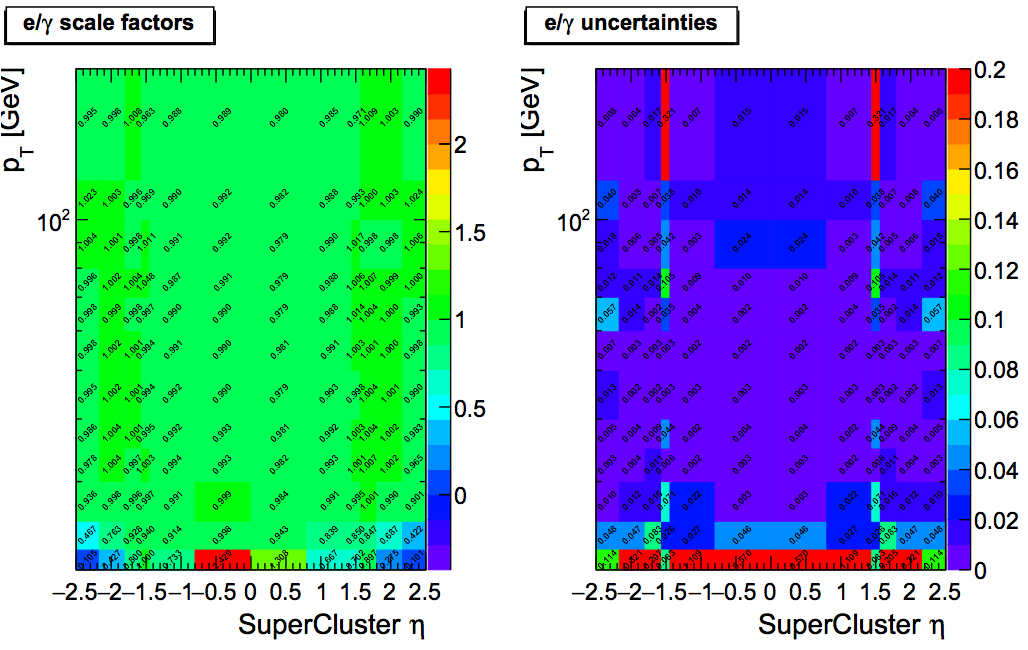
\includegraphics[width=1.0\textwidth]{trigger/electronTriggerEfficiencyelectronTriggerEfficiencyHLT_Leg1_WP90_2016.png} } \\
\subfloat Leg 2
{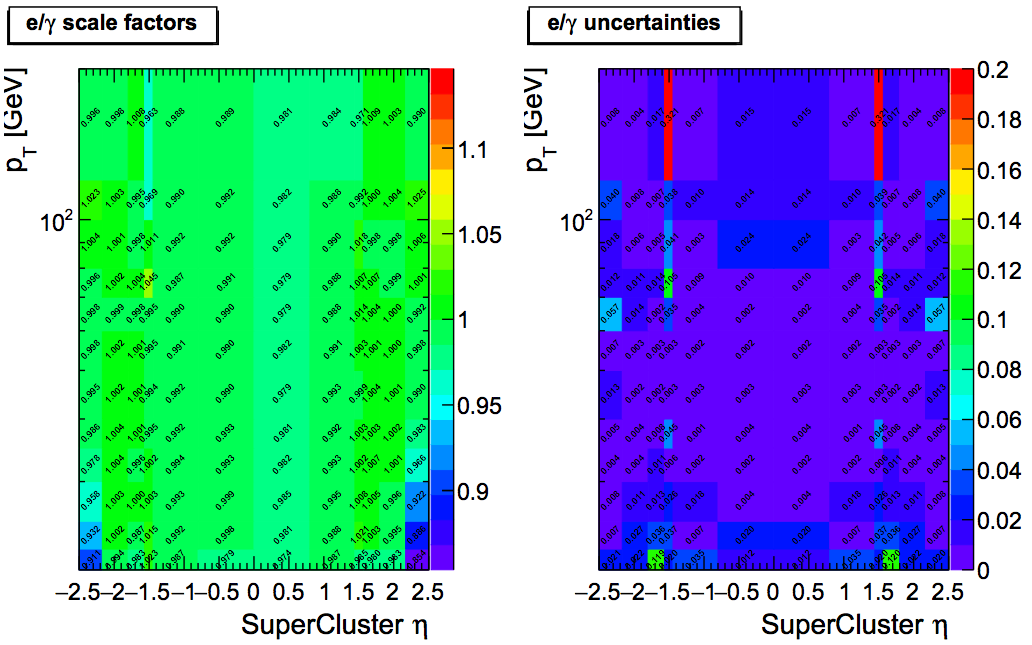
\includegraphics[width=1.0\textwidth]{trigger/electronTriggerEfficiencyelectronTriggerEfficiencyHLT_Leg2_WP90_2016.png} } \\
\caption{Electron scale factors in $p_{T}$ and $\eta$ bins for 2016 data set for the HLT\_Ele23\_Ele12\_CaloIdL\_TrackIdL\_IsoVL\_DZ trigger. ID cut (general purpose MVA WP90) and ISO cuts are applied, then the scale factors are measured. Taken from ~\cite{vhbbAN}}
\label{fig:trigger_eff_diele}
\end{figure}


\begin{figure}
\centering
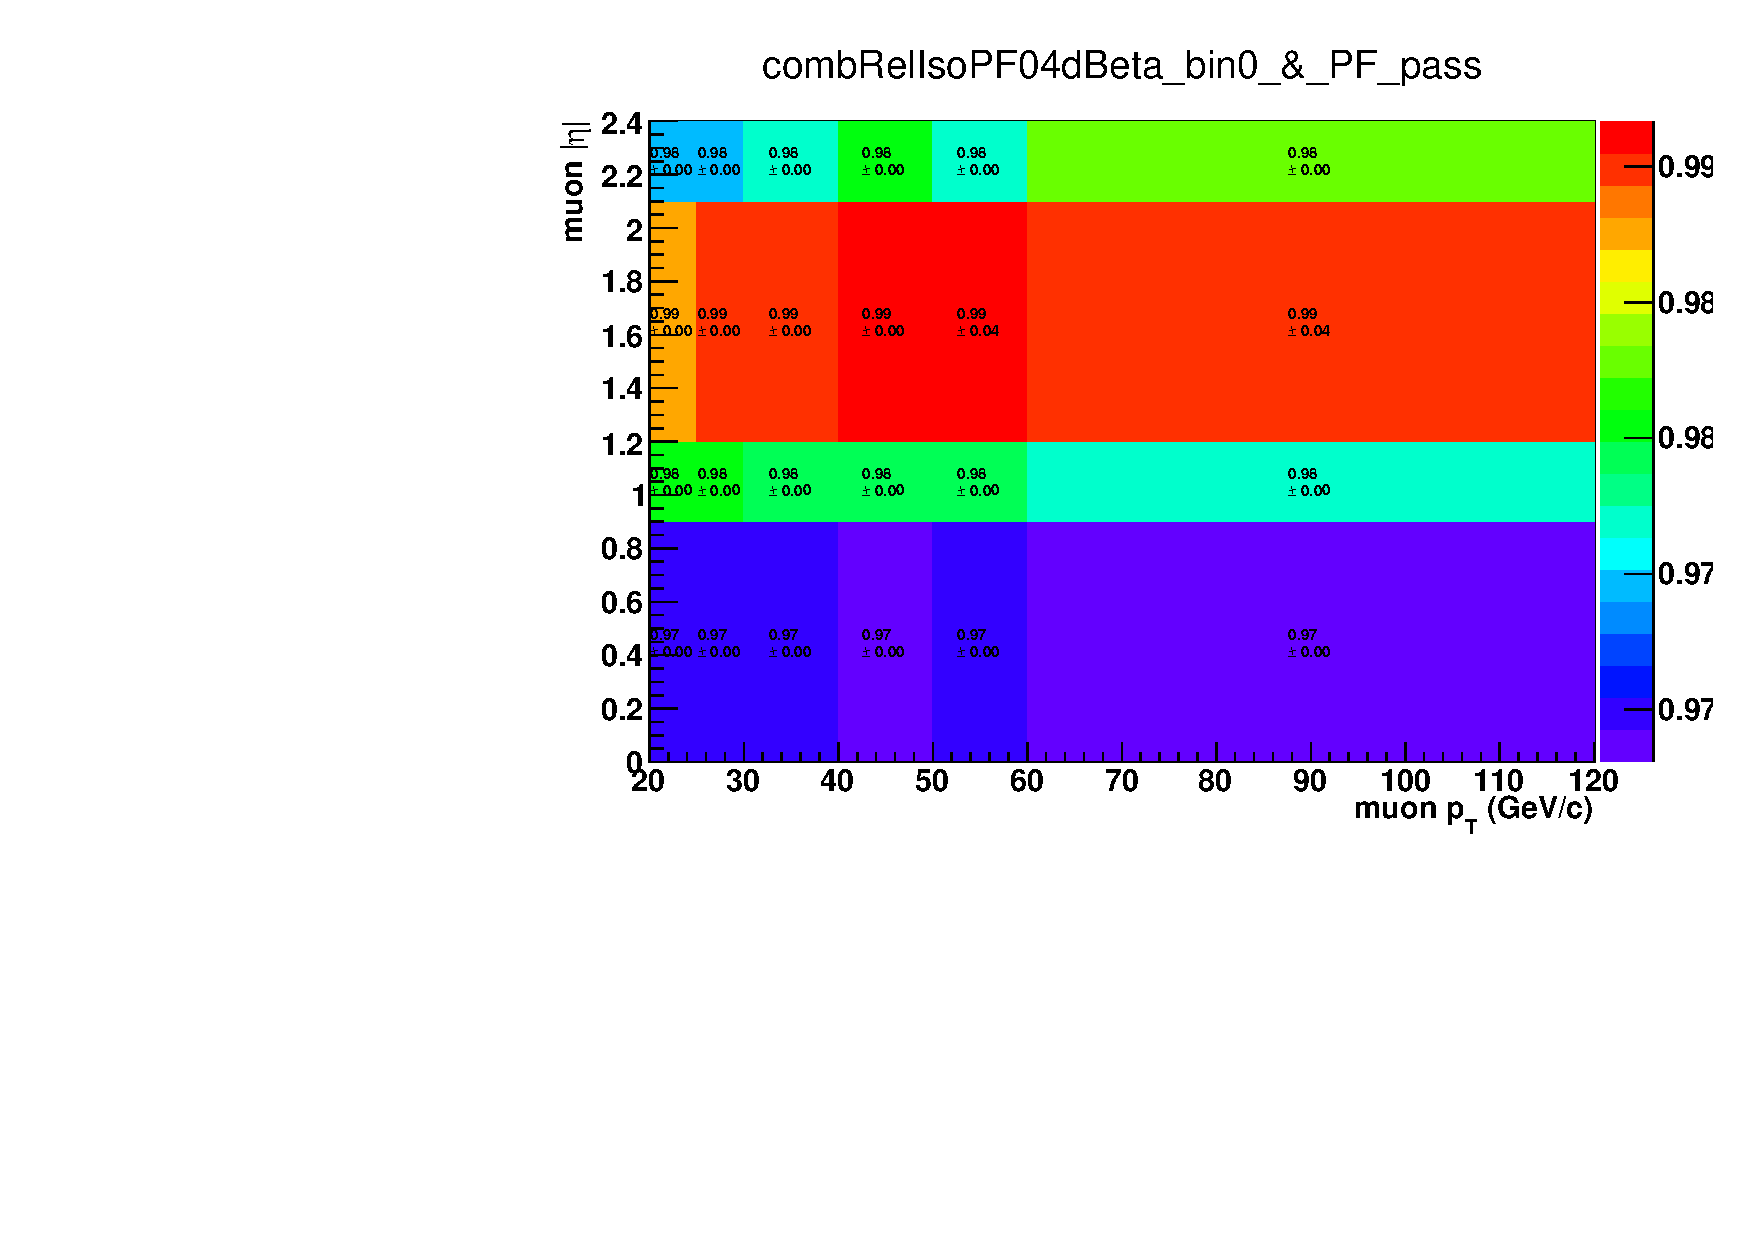
\includegraphics[width=0.475\textwidth]{trigger/Run_BCDEFG_PlotSF_hlt_Mu17_Mu8_OR_TkMu8_leg8_NUM_hlt_Mu17_Mu8_OR_TkMu8_leg8_DEN_LooseIDnISO_PAR_pt_eta_pt_abseta_ratio.pdf}
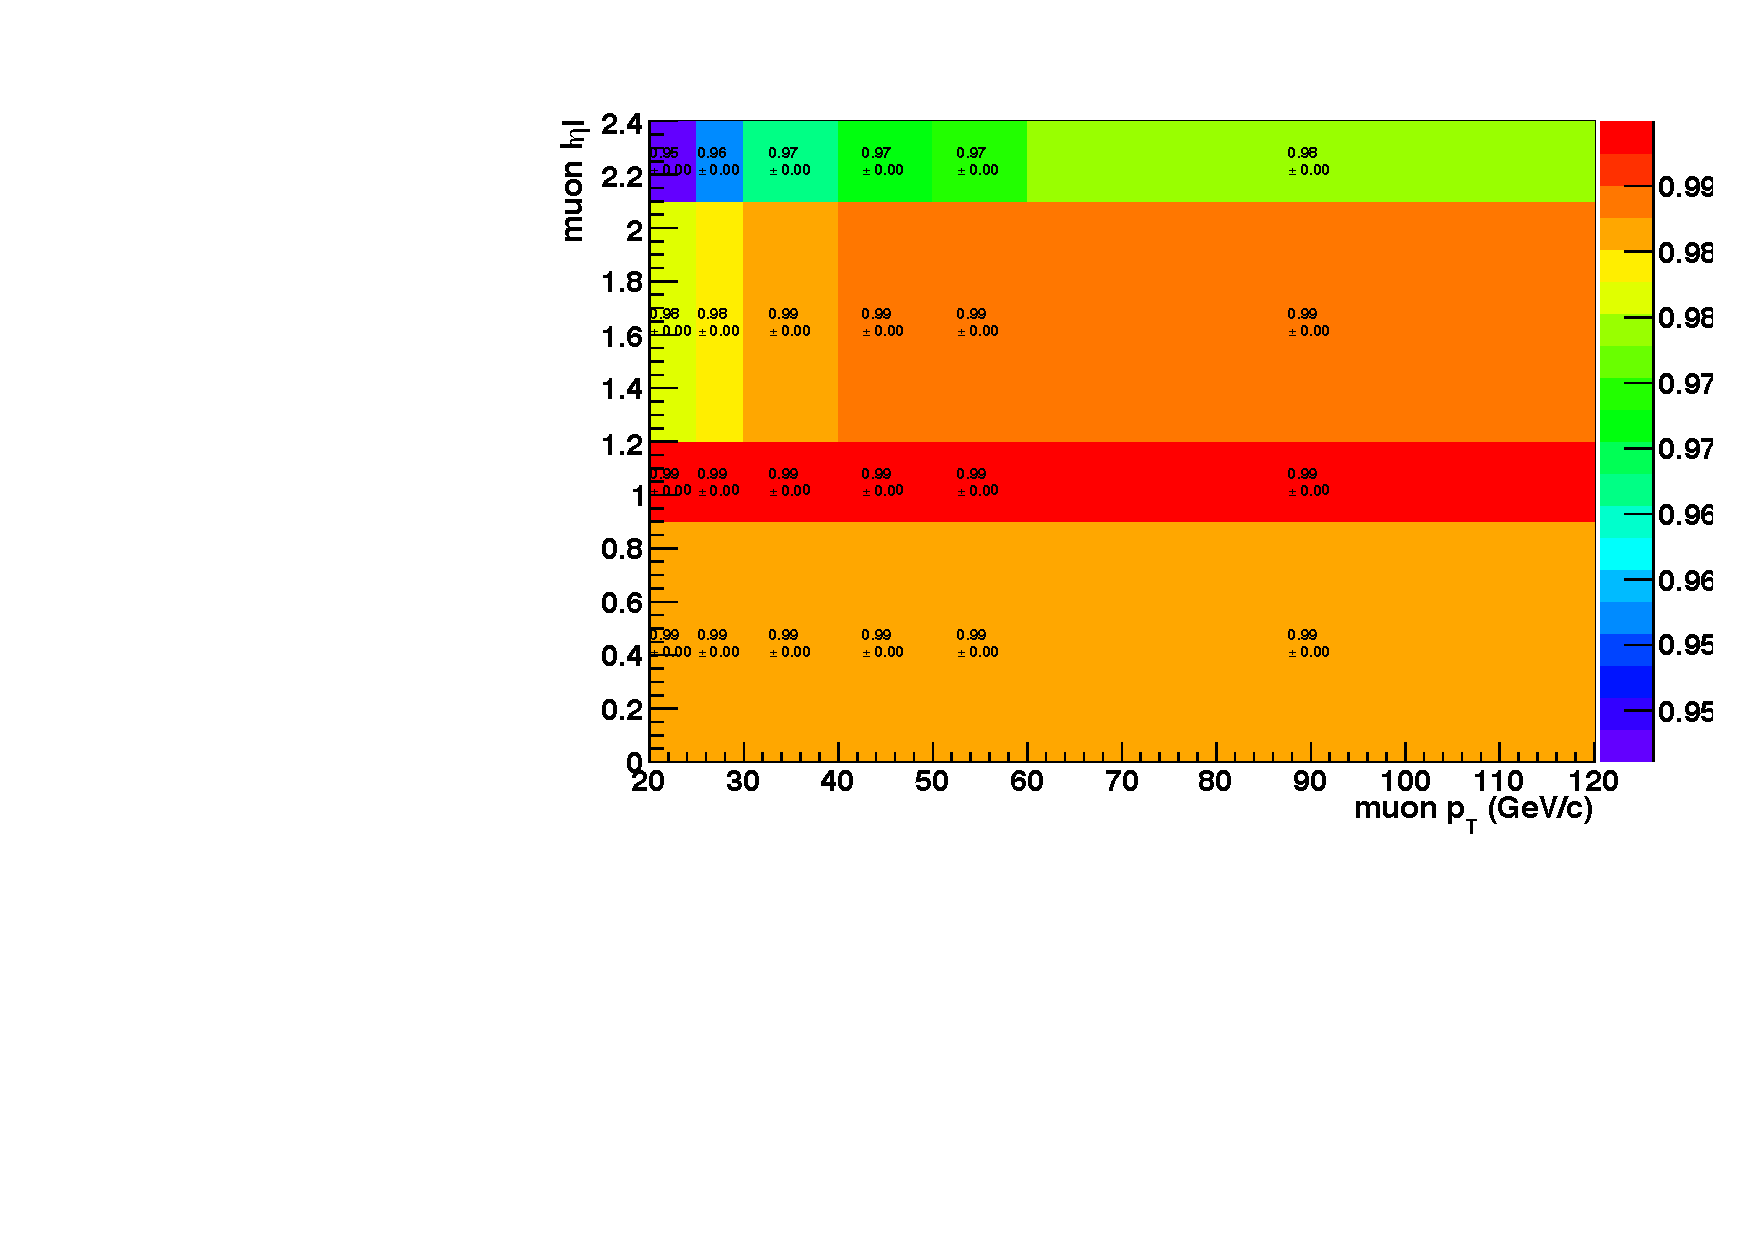
\includegraphics[width=0.475\textwidth]{trigger/Run_BCDEFG_PlotSF_hlt_Mu17Mu8_leg17_NUM_hlt_Mu17Mu8_leg17_DEN_LooseIDnISO_PAR_pt_eta_pt_abseta_ratio.pdf}\\
\caption{Muon scale factors in $p_{T}$ and $\eta$ bins for 2016 data runs B, C, D, E, F, G for the  HLT\_Mu17\_TrkIsoVVL\_Mu8\_TrkIsoVVL\_v* OR HLT\_Mu17\_TrkIsoVVL\_TkMu8\_TrkIs\
oVVL\_v* triggers. Left: Scale factors for 8 GeV leg. Right: Scale factors for 17 GeV leg, provided that the subleading leg passed 8 GeV cut.}
\label{fig:trigger_SF_dimu_BCDEFG}
\end{figure}

\begin{figure}
\centering
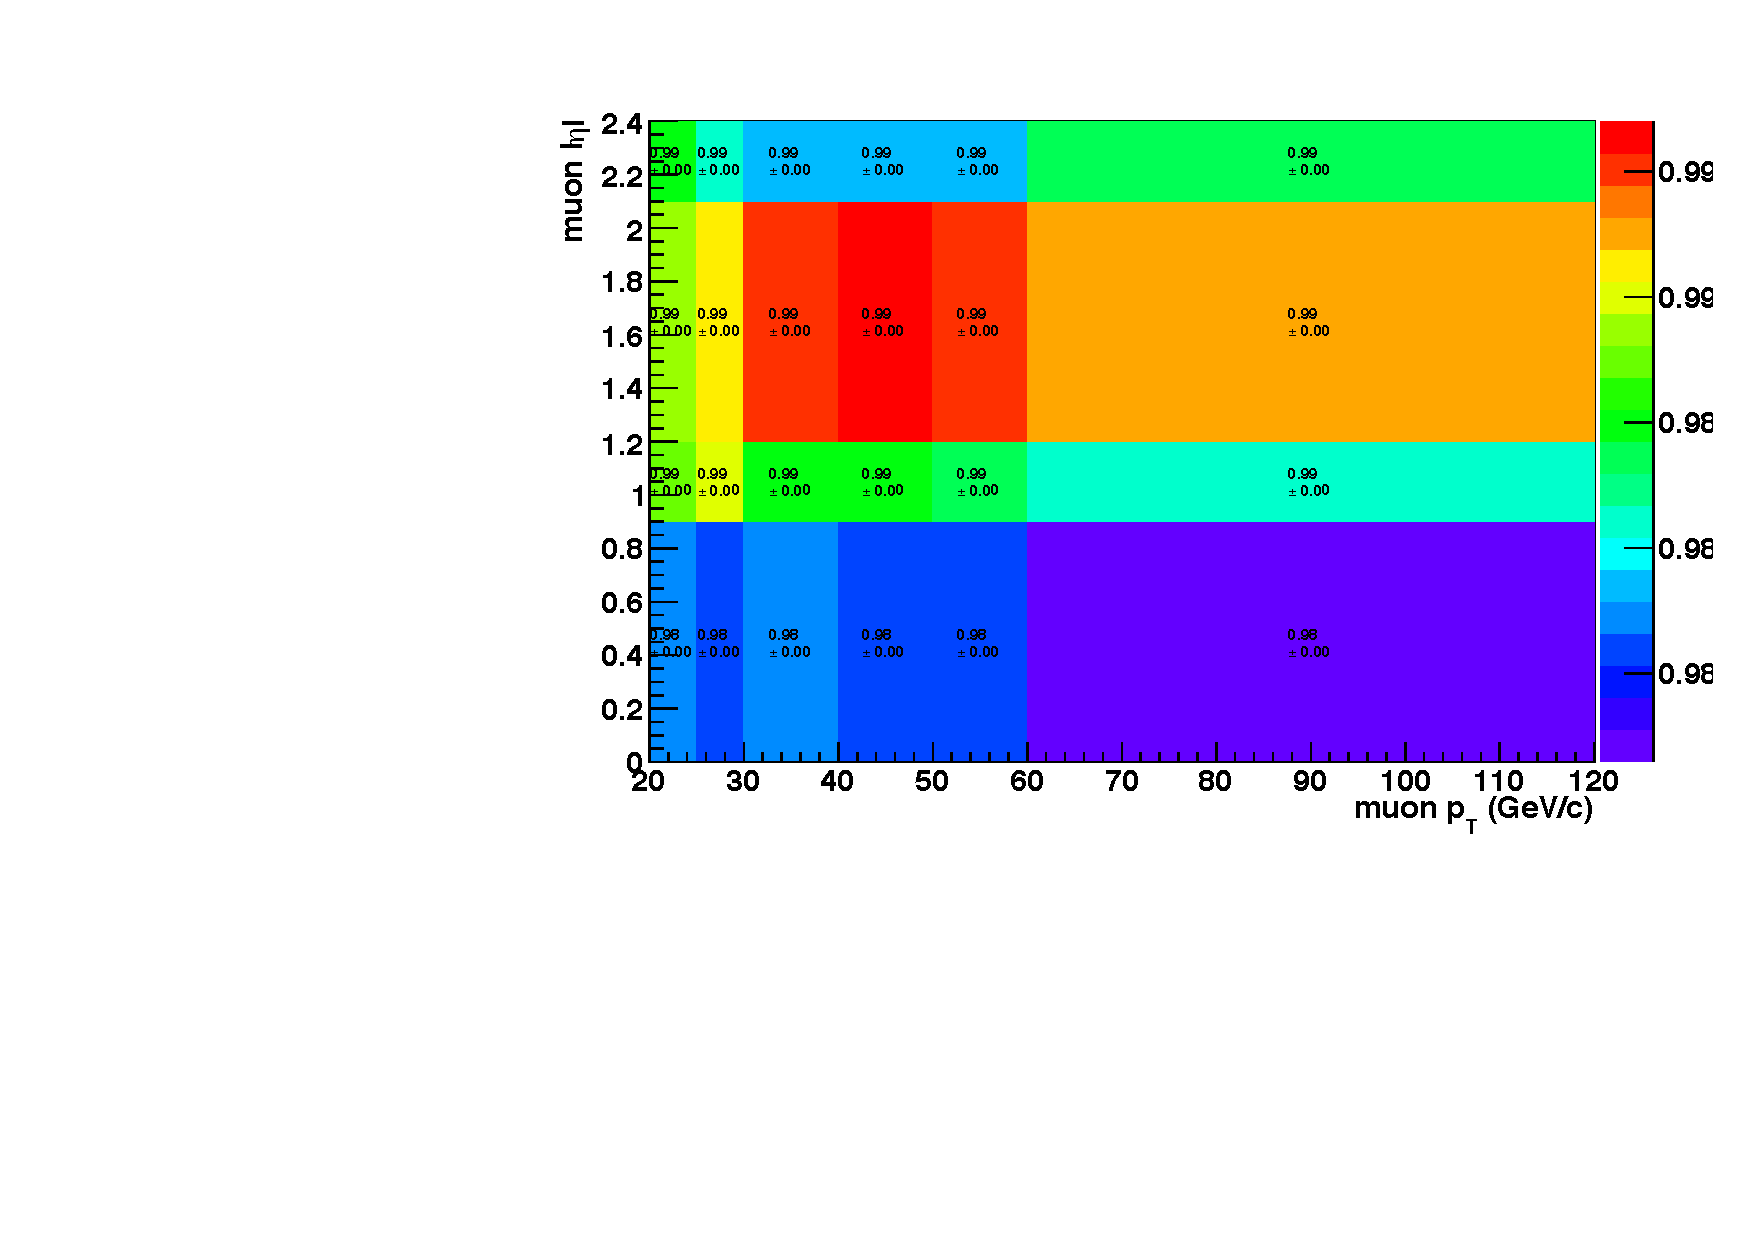
\includegraphics[width=0.475\textwidth]{trigger/Run_H_PlotSF_hlt_Mu17_Mu8_OR_TkMu8_leg8_NUM_hlt_Mu17_Mu8_OR_TkMu8_leg8_DEN_LooseIDnISO_PAR_pt_eta_pt_abseta_ratio.pdf}
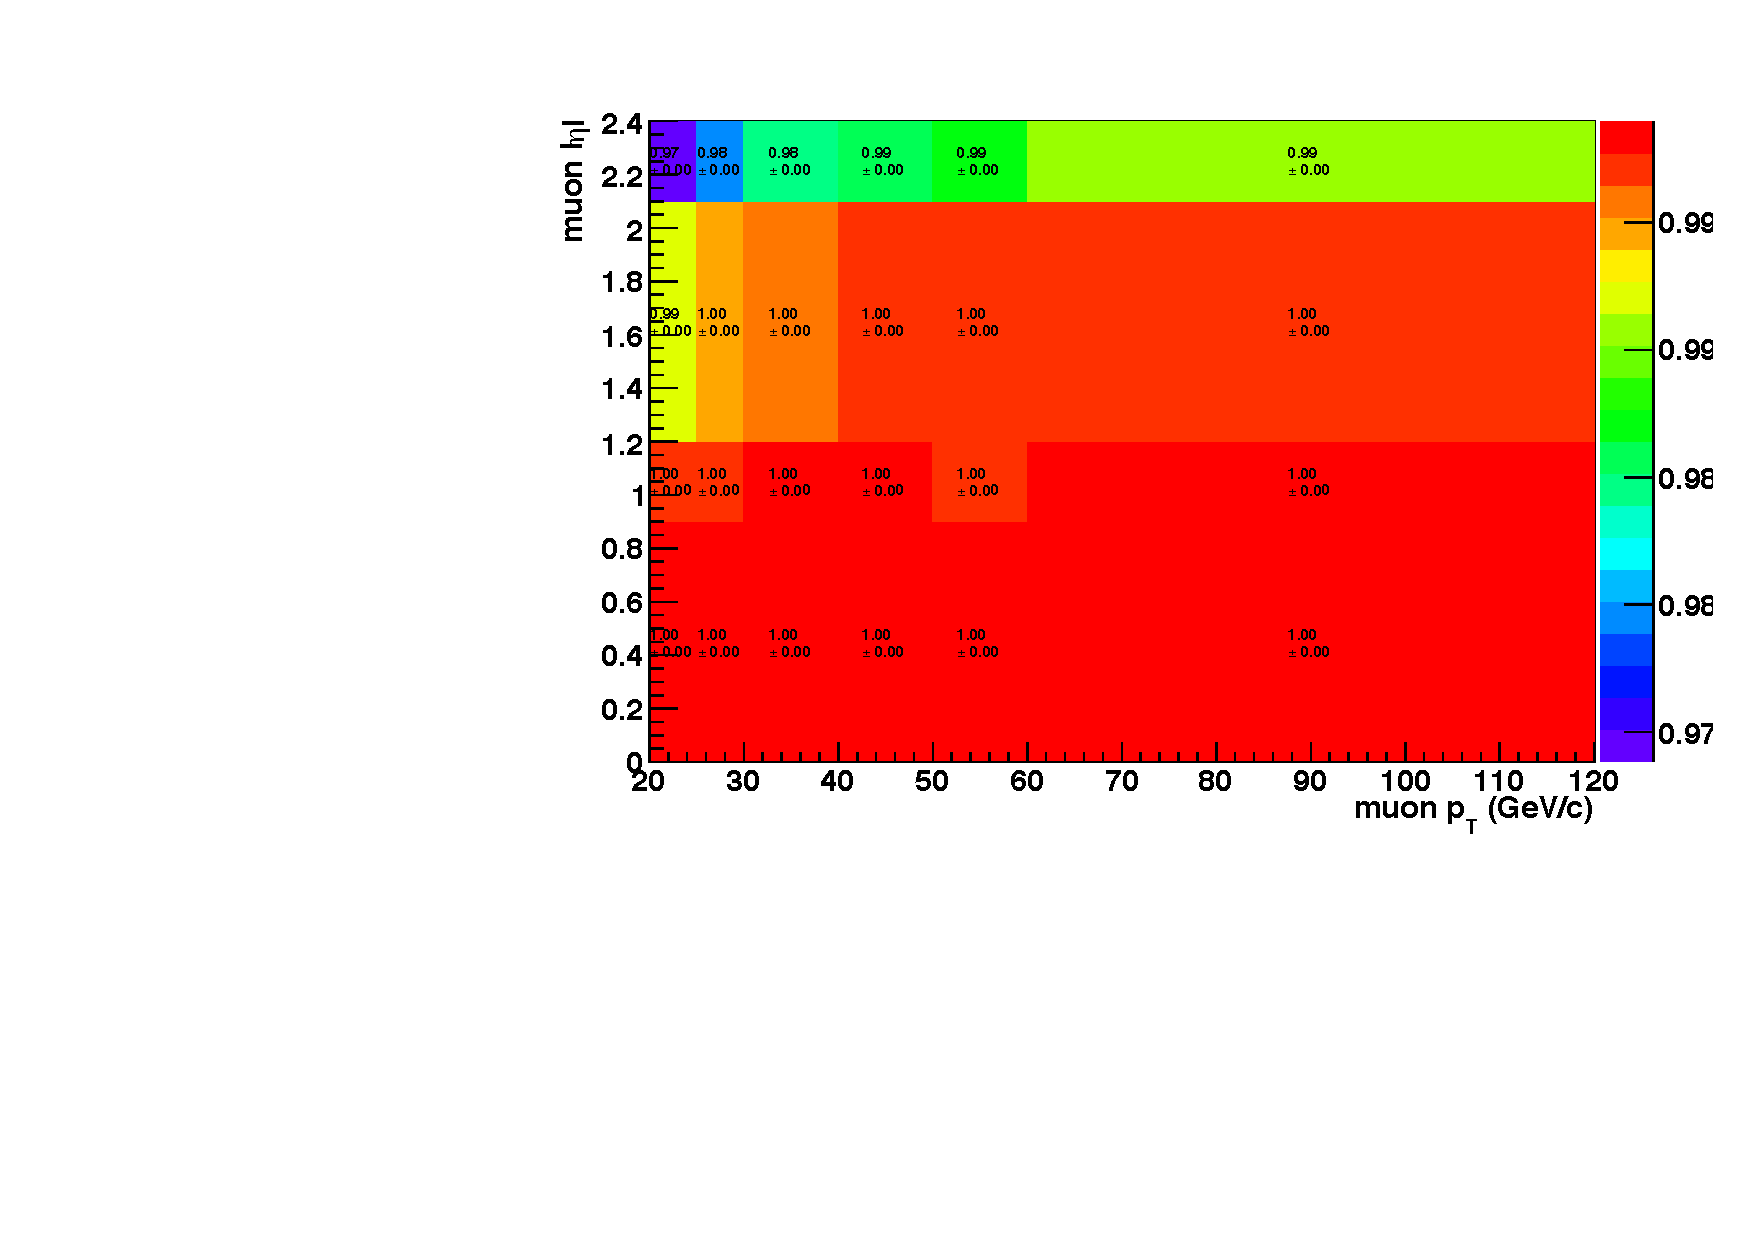
\includegraphics[width=0.475\textwidth]{trigger/Run_H_PlotSF_hlt_Mu17Mu8_leg17_NUM_hlt_Mu17Mu8_leg17_DEN_LooseIDnISO_PAR_pt_eta_pt_abseta_ratio.pdf}\\
\caption{Muon scale factors in $p_{T}$ and $\eta$ bins for 2016 data run H for the  HLT\_Mu17\_TrkIsoVVL\_Mu8\_TrkIsoVVL\_v* OR HLT\_Mu17\_TrkIsoVVL\_TkMu8\_TrkIs\
oVVL\_v* triggers. Left: Scale factors for 8 GeV leg. Right: Scale factors for 17 GeV leg, provided that the subleading leg passed 8 GeV cut.}

\label{fig:trigger_SF_dimu_H}
\end{figure}

\begin{figure}
\centering
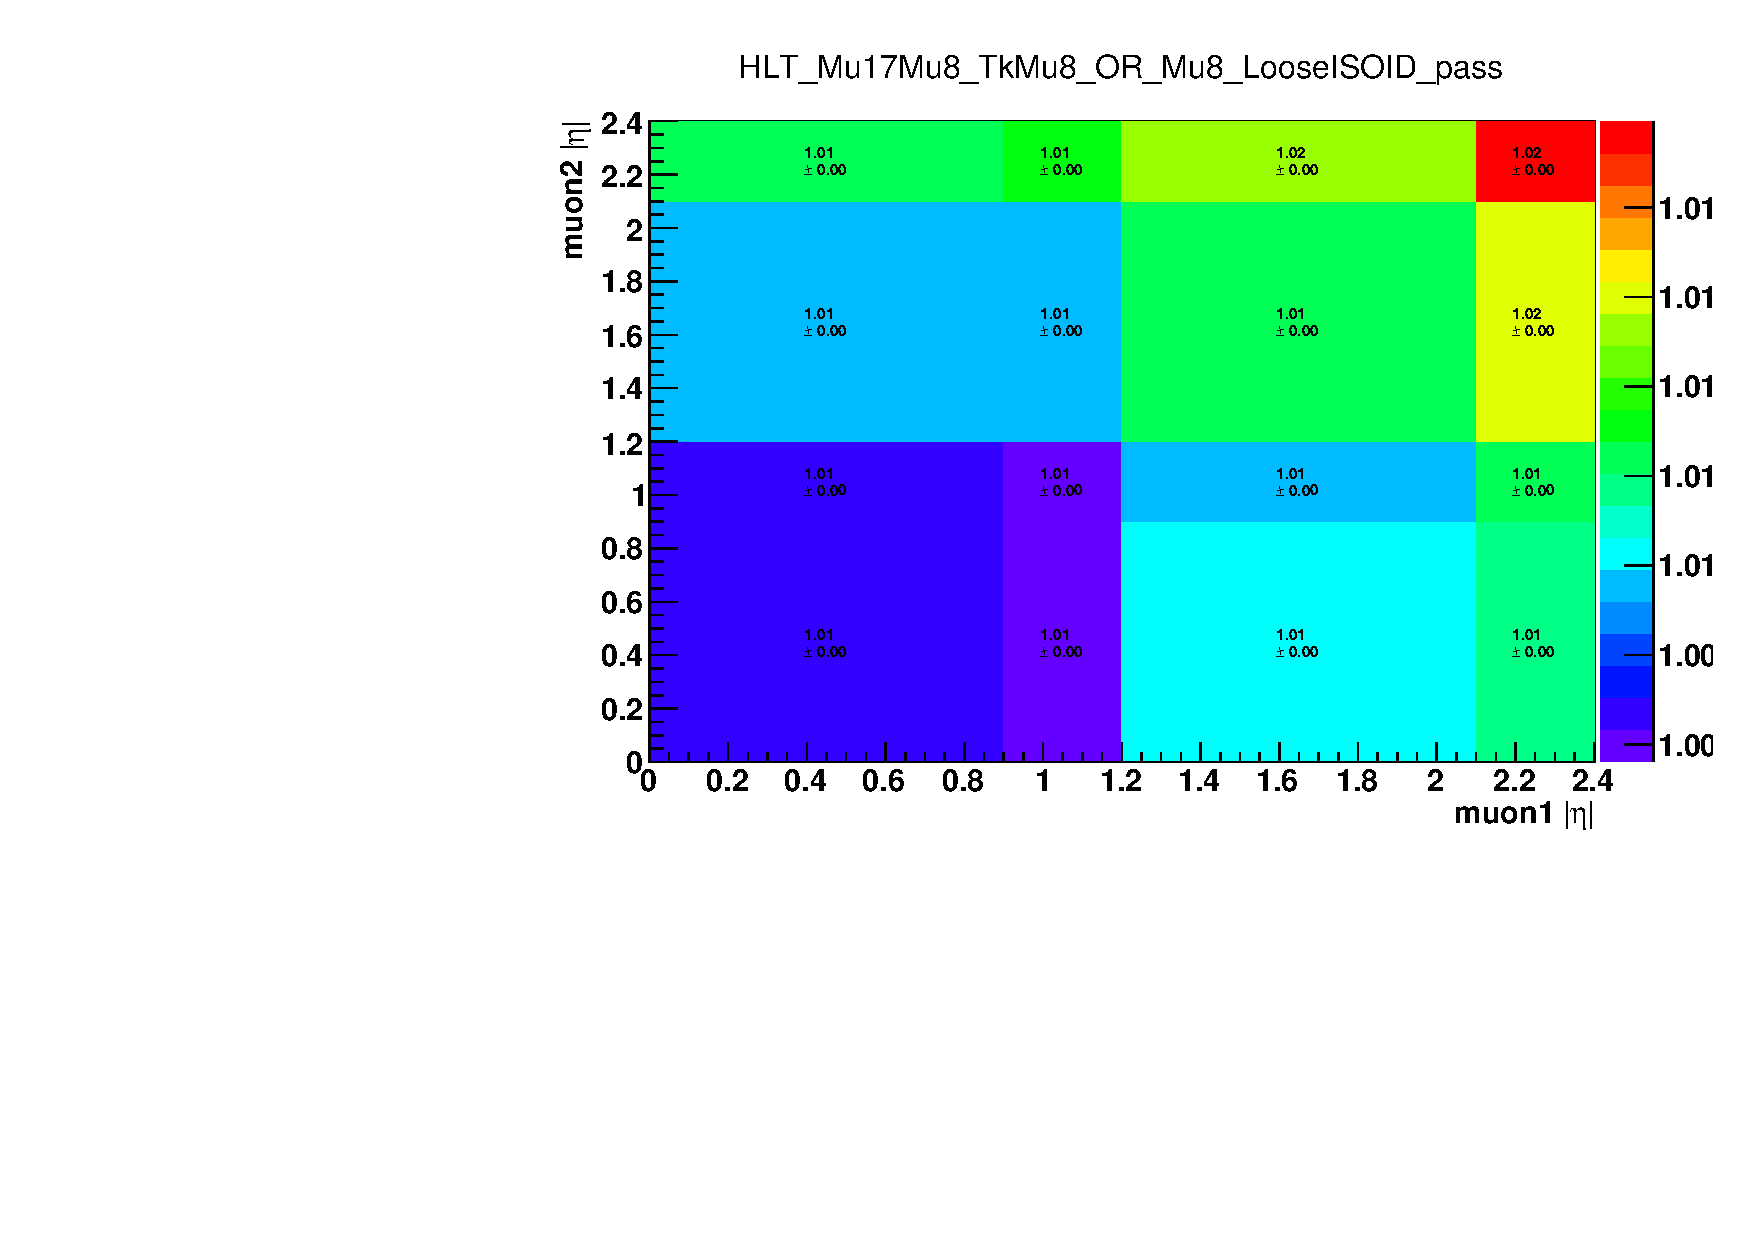
\includegraphics[width=0.85\textwidth]{trigger/PlotSF_dZ_NUM_dZ_DEN_hlt_Mu17_Mu8_OR_TkMu8_loose_PAR_eta1_eta2_abseta_tag_abseta_ratio.pdf}
\caption{Scale factors in $\eta$ bins of the leading and subleading muons for 2016 data set for dZ requirement, measured after muons have passed the HLT\_Mu17\_TrkIsoVVL\_Mu8\_TrkIsoVVL\_v* OR HLT\_Mu17\_TrkIsoVVL\_TkMu8\_TrkIsoVVL\_v* triggers. }
\label{fig:trigger_SF_dimu_dZ_H}
\end{figure}



\begin{figure}
\centering
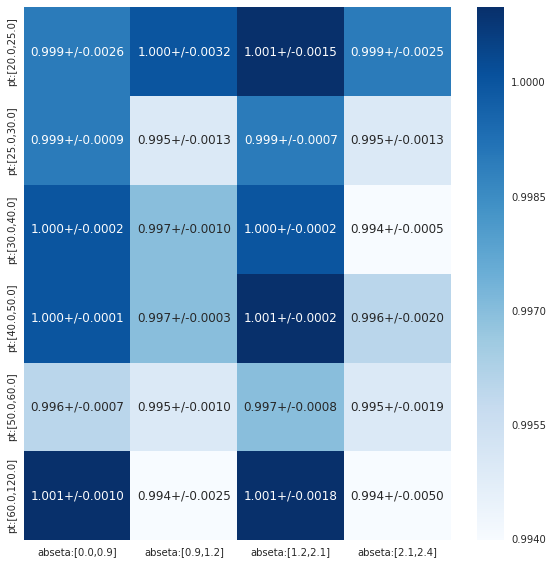
\includegraphics[width=0.5\textwidth]{muon_ID_BCDEFv2.png}
\bigbreak
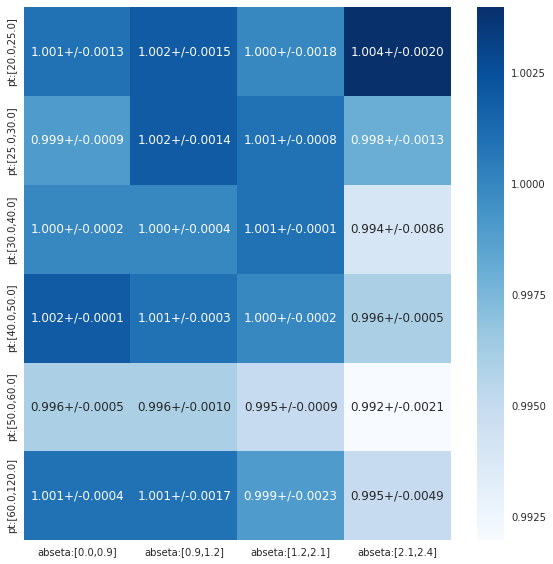
\includegraphics[width=0.5\textwidth]{muon_ID_GHv2.png}
\caption{ Muon ID scale factors in $p_{T}$ and $\eta$ bins. Left: runs B to F. Right: runs G and H.}
\label{fig:muonID_SF}
\end{figure}

\newline
\newline

\begin{figure}
\centering
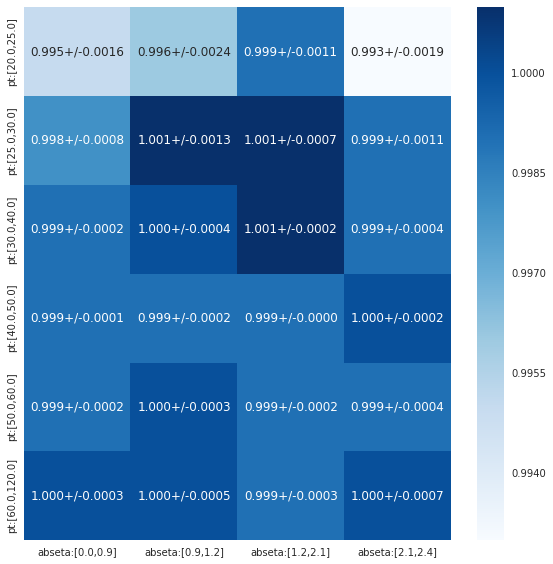
\includegraphics[width=0.5\textwidth]{muon_ISO_BCDEFv2.png}
\bigbreak
\includegraphics[width=0.5\textwidth]{muon_ISO_GHv2.png}
\caption{ Muon ISO scale factors in $p_{T}$ and $\eta$ bins. Left: runs B to F. Right: runs G and H.}
\label{fig:muonISO_SF}
\end{figure}

\newline
\newline

\begin{figure}
\centering
\includegraphics[width=0.9\textwidth]{EIDISO_ZH_out.png}
\caption{ Electron ID+ISO scale factors in $p_{T}$ and $\eta$ bins.}
\label{fig:muonID_SF}
\end{figure}

 \clearpage


%\subsection{Monte~Carlo samples\label{sec:mc}}

\subsection{Signal simulation\label{sec:signalMC}}

MC signal samples of the resonant Higgs boson pair production have been generated at the Leading Order (LO) using the \MADGRAPH~5 version\ ~2.2.2.0  generator ~\cite{Alwall:2014hca}. The gluon fusion production of a heavy narrow resonance is followed by the decay of the resonance into two SM Higgs bosons whose mass is fixed at 125~GeV.

Two signal MC samples are generated to cover the Higgs decay modes contributing to the 2 b jets 2 leptons 2 neutrinos final state of this measurement. The first sample type is a HH decay in to bbZZ channel, where one Higgs boson decays to a pair of b-quarks and the second Higgs boson decays into two Z bosons. In the second sample type bbVV events are generated, where HH can decay through bbWW and bbZZ channels. For both samples, the Z boson-pair and the W boson-pair are set to decay leptonically to two leptons and two neutrinos, where a lepton could be an electron or a muon. The second, bbVV, sample is filtered using the generator level information such that only the events with a W-boson pair (bbWW) are kept, while the Z-pair events are dropped: there are very few of them in the bbVV sample, and most importantly, high statistics bbZZ is taken from the dedicated bbZZ sample of the first type.

Events in the signal bbZZ and bbWW MC samples are normalised to 2~pb HH production cross section, which is a typical value of the heavy resonance production at 300 GeV predicted by the WED. Additionally the normalization includes the branching ratios of the Higgs boson decays contributing to the final state studied here: 0.0012 and 0.0266 for $HH\to bbZZ\to bb\ell\ell\nu\nu$ and $HH\to bbWW\to bb\ell\nu\ell\nu$, respectively \cite{CERNYR4}.

%%There are ten samples in the mass range of 260 to 1000 GeV generated for bbVV analysis and 16 samples for bbZZ from 250 GeV to 1000 GeV. Therefore, this document presents results for the masses where both signals are present. In the future we would consider doing approximations of the bbWW contribution where we have missing samples or generate them privately.

Unless mentioned otherwise, throughout the text plots and numbers represent the graviton study. The data and backgrounds for the radion measurement are the same, thus distributions also show the same good Data MC agreement and can be found for at Figs. ~\ref{fig:MCcomparisons} for the graviton case and ~\ref{fig:MCcomparisons_radion} for the radion case.

\subsection{Background simulation\label{sec:bkgMC}}

In this analysis the main backgrounds are \ttbar and Drell-Yan plus
jets with the mass of the boson greater than 50 GeV. Not all the
background processes pass our tight preselection (see section ~\ref{hhSelection}),
those which do, are single top, dibosons, and ZH backgrounds that are
listed in the Table \ref{tab:bg_mcsamples}:

\begin{table}[htbp]%H]
  %\footnotesize
  \begin{center}
    \caption{Background Monte Carlo samples\label{tab:bg_mcsamples}}
    \begin{tabular}{|c|}%|l|r|r|r|r|r|}
      \hline
      % Sample  & Generator & $m_{H} (\GeV/c^2)$ & $\sigma$ (pb) & events &  $\int\cal L$ (\fbinv) \\
      %\hline
      \multicolumn{5}{|l|}{\texttt{DY1JetsToLL\_M-50\_TuneCUETP8M1\_13TeV-madgraphMLM-pythia8}} \\
%                & \MADGRAPH\,5+\PYTHIA{}\,8 & 725 & 39 800 000 & 54.5 \\
      \multicolumn{5}{|l|}{\texttt{DY2JetsToLL\_M-50\_TuneCUETP8M1\_13TeV-madgraphMLM-pythia8}} \\
%               & \MADGRAPH\,5+\PYTHIA{}\,8 & 725 & 39 800 000 & 54.5 \\
      %\hline
      \multicolumn{5}{|l|}{\texttt{DY3JetsToLL\_M-50\_TuneCUETP8M1\_13TeV-madgraphMLM-pythia8}} \\
%              & \MADGRAPH\,5+\PYTHIA{}\,8 & 394.5 & 19 400 000  & 50.2 \\
      %\hline
      \multicolumn{5}{|l|}{\texttt{DY4JetsToLL\_M-50\_TuneCUETP8M1\_13TeV-madgraphMLM-pythia8}} \\
%             & \MADGRAPH\,5+\PYTHIA{}\,8 & 96.47 & 4 960 000 & 52.2 \\
      \multicolumn{5}{|l|}{\texttt{WW\_TuneCUETP8M1\_13TeV-pythia8}} \\
%            & \PYTHIA{}\,8 & 118.7 & 993 640 &  8.37  \\
      %\hline
      \multicolumn{5}{|l|}{\texttt{WZ\_TuneCUETP8M1\_13TeV-pythia8}} \\
%           & \PYTHIA{}\,8 & 47.13    &   1 000 000   &   21.22  \\
      %\hline
      \multicolumn{5}{|l|}{\texttt{ZZ\_TuneCUETP8M1\_13TeV-pythia8}} \\
%          & \PYTHIA{}\,8 & 16.523     &   985 600   &   59.65  \\
       \multicolumn{5}{|l|}{\texttt{ZH\_HToBB\_ZToLL\_M125\_13TeV\_aMC@NLO}} \\
      %\hline
      \multicolumn{5}{|l|}{\texttt{TT\_TuneCUETP8M1\_13TeV-powheg-pythia8}} \\
       %         & \POWHEG+\PYTHIA{}\,8 & 831.76   & 187 626 200 + 97 994 442&  343  \\
      %\hline
      \multicolumn{5}{|l|}{\texttt{ST\_tW\_top\_5f\_inclusiveDecays\_13TeV-powheg-pythia8\_TuneCUETP8M1}} \\
        %        & \POWHEG+\PYTHIA{}\,8 & 35.6   &   1 000 000   &   28.09  \\
      %\hline
      \multicolumn{5}{|l|}{\texttt{ST\_tW\_antitop\_5f\_inclusiveDecays\_13TeV-powheg-pythia8\_TuneCUETP8M1}} \\
         %       & \POWHEG+\PYTHIA{}\,8 & 35.6   &   999 400   &   28.07  \\
      %\hline\hline
      \multicolumn{5}{|l|}{\texttt{ST\_t-channel\_top\_4f\_leptonDecays\_13TeV-powheg-pythia8}} \\
          %      & \POWHEG+\PYTHIA{}\,8 & 136*0.325   &   999 400   &   22.6 \\
      %\hline
      \multicolumn{5}{|l|}{\texttt{ST\_t-channel\_antitop\_4f\_leptonDecays\_13TeV-powheg-pythia8}} \\
           %     & \POWHEG+\PYTHIA{}\,8 & 81*0.325   & 1 695 400 &  64.4 \\
      %\hline\hline
      \multicolumn{5}{|l|}{\texttt{ST\_s-channel\_4f\_leptonDecays\_13TeV-amcatnlo-pythia8}} \\
      %    & \POWHEG+\PYTHIA{}\,8 & 10.32   &   998 400   &   96.74  \\
\hline%\hline

    \end{tabular}
  \end{center}
  %\label{backgrounds} 
\end{table}



The simulated samples of the background processes such as 
~\ttbar~\cite{Frixione:2007nw} and the single top tW and t-channel
production processes~\cite{Frederix:2012dh} are generated at the
next-to-leading order (NLO) with POWHEG~\cite{Alioli:2009je}, while
single top s-channel production process is generated at NLO with
\MADGRAPH. \ttbar and single top production cross sections are
rescaled to the next-to-next-to-leading order (NNLO). 
Drell-Yan (DY)
process samples in association with 1, 2, 3 or 4 jets are generated
at the leading order using \MADGRAPH with the MLM
matching~\cite{Alwall:2007fs} and rescaled to NNLO using~\textsc{fewz}
program~\cite{Gavin:2010az,Li:2012wna,Gavin:2012sy}. 

As for the electroweak (EWK) order, DY samples have been rescaled to EWK NLO order with the NLO/LO k-factor of 1.23~\cite{DYkfactor}. Diboson samples
are generated at LO with {\PYTHIA}8.212~\cite{Sjostrand:2007gs}.

The main background
       process, which involves SM Higgs boson, is an associated
       production of the Higgs boson with a Z boson (ZH).  ZH process
       is simultated using the generator
%{{\sc MadGraph5_aMC@NLO}}                                                                                                                                                                               
$MadGraph5\_aMC@NLO$
~\cite{cite_aMC@NLO} with FxFx
merging~\cite{Frederix:2012ps} and
rescaled to NNLO with
{\MCFM} generator~\cite{Campbell:2010ff}.


For LO and NLO samples NNPDF3.0 parton distribution functions (PDF)
set is used. {\POWHEG} and {\MADGRAPH} interfaced with
{\PYTHIA}8.212~\cite{Sjostrand:2007gs} are used for the parton
showering and hadronization steps. To describe the underlying event
CUETP9M1 set derived in \cite{Khachatryan:2015pea} is
used. \GEANTfour~\cite{GEANT4} is used to model the response of the
CMS detector.

All the final cross sections denoted as NNLO are calculated at NNLO QCD accuracies and have been computed with the tool they were generated with. They found to be in agreement with the values from the LHC Higgs cross section working group ~\cite{LHCHXSWG, xsecZH, xsecTT, xsecST, xsecVV}.

During the data taking in 2016 the average number of proton-proton interactions per bunch crossing was 24 (denoted as pile up later), and in MC samples this information has been introduced overlapping these interactions with the events of interest.



 \clearpage

The bbZZ analysis uses the standard set of the CMS
reconstructed physics objects. We describe reconstruction of
electrons, muons, jets and b jets, and MET separately below:



\subsection{Electrons\label{sec:electrons}}
The Gaussian Sum Filter algorithm (GSF
Electrons)~\cite{Khachatryan:2015hwa} is used to reconstruct
electrons. The measurement selects electrons, which pass the following selection:
%loose set of preselection cuts in applied,
%namely, 
leading electron $\pt>25\GeV$ and subleading electron $\pt>15\GeV$, $|\eta|<2.5$, 
%$d_{xy}<0.05\cm$, $d_z<0.2\cm$ and 
an isolation cut of 0.06, for which the cone
of $0.3$ is used to compute the $\rho$-subtracted PF
isolation.  Lepton isolation is calculated as a scalar sum of
the transverse momentum $(p_{T})$ of all the charged and
neutral hadrons as well as photons around the lepton
(excluding the cone) divided by the $p_{T}$ of the lepton
itself. 
%POG recommended MVA ID WP Loose is further applied to the set of selected electrons.
%The cut on isolation in the measurement for electrons is $0.06$.

        
        %%To emulate the conditions of the HLT trigger, a set of offline cuts is applied further.

%% \texttt{pt>15 \& (}\\
%% \texttt{(abs(superCluster().eta)<1.4442 \& full5x5\_sigmaIetaIeta<0.012 \& }\\
%% \texttt{hcalOverEcal<0.09 \&}\\
%% \texttt{(ecalPFClusterIso/pt)<0.4 \& (hcalPFClusterIso/pt)<0.25 \&}\\
%% \texttt{(dr03TkSumPt/pt)<0.18 \& abs(deltaEtaSuperClusterTrackAtVtx)<0.0095 \&}\\
%% \texttt{abs(deltaPhiSuperClusterTrackAtVtx)<0.065) || }\\
%% \texttt{(abs(superCluster().eta)>1.5660 \& full5x5\_sigmaIetaIeta<0.033 \&}\\
%% \texttt{hcalOverEcal<0.09 \&}\\
%% \texttt{(ecalPFClusterIso/pt)<0.45 \& (hcalPFClusterIso/pt)<0.28 \&}\\
%% \texttt{(dr03TkSumPt/pt)<0.18)}\\
%% \texttt{).}

        In addition, a specific POG recommended working point is applied, which is a multivariate analysis (MVA) based criteria for classification of signal/background electrons. For this analysis we use the loose working point (another name can be WP90), as described in ~\cite{vhbbAN}. ID and ISO, as well as HLT SFs are applied.
%        \small{\texttt{https://twiki.cern.ch/twiki/bin/viewauth/CMS/ \\MultivariateElectronIdentificationRun2}}
%\normalsize



\subsection{Muons\label{sec:muons}}
        In this analysis we are using global muons reconstructed using the information from the tracker and muon-chamber \cite{CMS-PAS-MUO-10-002,Chatrchyan:2012xi}. The selection of muons is:
leading muon $\pt>20\GeV$ and subleading muon $\pt>15\GeV$, $|\eta|<2.4$,
%re is a loose preselection of $\pt>5\GeV$, $|\eta|<2.4$, $d_{xy}<0.5\cm$, $d_z<1.0\cm$, as well as 
a relative
isolation cut of 0.15, with the cone of $0.4$ used to compute $\Delta\beta$-subtracted PF isolation.
Finally, a tighter selection - POG recommended WP Loose is applied.~\cite{MuonsRun2}. ID, ISO, HLT and traker SFs are applied.
%The offline cut on isolation for muons is $0.15$.
%% Loose muon:
%% \begin{itemize}
%%   \item  Particle-Flow Muon:\\
%% \texttt{isPFMuon()}
%%   \item  is Global or Tracker Muon:\\
%% \texttt{isGlobalMuon() || isTrackerMuon()}
%%  \end{itemize}







\subsection{Jets\label{sec:jets}}
    Particle flow algorithm is used to reconstruct jets\cite{CMS-PAS-PFT-09-001,CMS-PAS-PFT-10-001}, with the help of the  $\text{anti}-k_T$ clustering algorithm having a distance parameter of $R=0.4$~\cite{Cacciari:2005hq,Cacciari:2008gp}.
    Reconstructed jets are further corrected for detector effects using specific correction determined from the data and MC. Only jets passing $|\eta|<2.4$ and  $(\pt > 30\GeV)$ are considered for the analysis. 
    All the necessary jet energy resolution (JER) and jet energy scale (JES) corrections provided by the JetMET group are applied ~\cite{JetMETgroup}.

%following this twiki:
%\begin{center}
 %   \texttt{https://twiki.cern.ch/twiki/bin/viewauth/CMS/JetResolution}    
%\end{center}






\subsection{Identification of b jets\label{sec:bjets}}
MVA technique combining the information about the impact parameter, identified secondary vertices, as well as soft lepton (if any) contained inside of the jet is used by the CMVA algorithm to identify b quark originated jets. The output is a continuous MVA discriminant ranging in value from -1 to +1. Optimal cut is determined by the POG for several working points. We use CMVAv2 medium working point  $(>0.4432)$. We checked all three WPs and WP Medium gives the best limits. b tag and mistag corrections are applied.

%\clearpage


\subsection{Missing transverse energy}\label{sec:MET}

MET type-1 corrected is calculated as an absolute value of the negative vector sum of all the visible PF candidates in the event. Then all the necessary corrections recommended by the POG are applied ~\cite{MissingETRun2Corrections} and on top, a set of filters related to the instrumental effects is employed ~\cite{MissingETOptionalFiltersRun2}. 
%following the twiki:
%\begin{center}
%\texttt{https://twiki.cern.ch/twiki/bin/viewauth/CMS/MissingETRun2Corrections}
%\end{center}
%On top, a set of filters related to the instrumental effects is employed:
%\begin{center}
%\texttt{https://twiki.cern.ch/twiki/bin/view/CMS/MissingETOptionalFiltersRun2}
%\end{center}
 \clearpage

%Two analysis methods are pursued to select samples that can be 
%used to extract the signal yield from the data in an optimal way.
\subsection{Higgs and Z Boson Selection}

Only dilepton pairs having net charge of zero are considered as \ZtoLL~ candidates. 
Pairs of prompt isolated leptons have to have a dilepton mass greater \
than 76 GeV. This ensures the orthogonality with HIG-17-006 bbVV analysis (later also referred to as bbWW analysis) as well as helps selecting decays of real Z bosons.

Higgs boson decays are reconstructed from the b jet pairs utilising only the two with the highest CMVAv2 discriminant value. We do not veto additional b jets. 

Double Higgs object is computed as a sum of Lorentz vectors of the \ZtoLL~ candidate, MET, and a \HBB~ candidate. Then, we compute the transverse mass of that object.

Transverse mass definition that we follow is one of the commonly used and is logical in the sense that we subtract the longitudinal momentum component which leaves us with the transverse momentum components only (while the energy remains the total energy).

More precisely, as the z-component of the neutrinos' momentum is unknown, we form a pseudo transverse mass:

%$M_T...with-tilda = $ (further referred as transverse mass for brevity), where E and pz are the energy and momentum of the candidate defined above.''                \
                                                                                                                                                                       

$\tilde{M}_T(HH) = \sqrt{E^2 - p_{z}^2}$ (further referred as transverse mass for brevity), where $E$ and \
$p_z$ are the energy and the Z-axis component of the Lorentz energy-momentum vector of the HH candidate.

The resulting distribution is what will be used in the binned shape analysis with the Higgs Combination Tool following the section ``Binned shape analysis'' as described at the twiki~\cite{CombinedLimit}.

%:
%\begin{center}
%    \small{\texttt{https://twiki.cern.ch/twiki/bin/view/CMS/SWGuideHiggsAnalysisCombinedLimit}}
%\end{center}

Analysis preselection to reduce ntuples size starts with the requirement on dilepton mass \toprule
 be greater than 50 GeV and the event to contain at least two jets with $p_{T} > 30$ GeV and $|\eta| < 2.4$. In addition to requirements on Higgs bosons decaying to b quarks mentioned above, we define Z bosons as two opposite sign muons with $p_{T} > 20/15$ GeV or two opposite sign electrons with $p_{T} > 25/15$ GeV. 



Later analysis cuts to improve signal-background separation include: the requirement on at least two b jets in the event, out of which two with the highest CMVAv2 score are used to define \HBB ~candidate. The lower end cut on the \HBB mass is set to 20 GeV to remove the low mass resonances while giving BDT as many events in the CRDY as possible at the same time. The upper end cut is not explicitly set for the same purpose. The actual \HBB mass distribution after the analysis selection is concentrated in the range 30 to 220 GeV. Then the Z boson selection cut takes the most energetic two leptons of the opposite sign and requires the their dilepton mass to pass 76 GeV < Z mass < 106 GeV selection used for the signal region definition. This is a standard +- 15 GeV window for Z boson selection whose lower end also preserves othogonality with the existing HIG-17-006 bbVV analysis. HH candidate is approximated by the sum of \ETslash, Z, and \HBB decays. A loose cut on HH transverse \textgreater~ 100 GeV removes evidently background events. Finally, an additional set of \ETslash cuts is used to ensure orthogonality with the existing HIG-18-013 bbZZ analysis focusing on the 2b jets + 2 leptons + 2 quarks, see Table \ref{metCuts}:


\begin{table}
\begin{center}
\caption{\ETslash cut to orthogonalise the analysis with respect to HIG-18-013.}
\begin{tabular}{|c|c|} \hline
{Signal mass, GeV} &  \ETslash cut, GeV\\\hline
260-300     &                                \textgreater~40 \\
350-600     &                                \textgreater~75 \\
650-1000    &                                \textgreater~100 \\
\hline
\end{tabular}
\label{metCuts}
\end{center}
\end{table}



\subsection{\HBB ~and \ZtoLL ~variables to define signal and control regions}

In this analysis we define three regions in the \HBB ~and \ZtoLL
~space. Two regions, CRDY and CRTT, are used to extract the
normalization of corresponding backgrounds. Signal region (Fig. ~\ref{fig:regions}) is chosen by
the set of \HBB~and \ZtoLL ~cuts \ref{fig:regions}. To reduce background contamination in this region, an additional cut on the MVA output is used. Boosted decision trees (BDT) MVA technique is employed to
separate background from signal. Below we describe in details
selection of each region and BDT construction. 

%% Skimming is applied
%% before building BDT to remove unnecessary background, while still
%% keeping a lot of events for BDT training. The set of "HH loose
%% common-sense" \label{hhSelection} skimming/preselection cuts includes: Dilepton (ee/mm)
%% mass $>$ 50 GeV, 2 or more jets: pt $>$ 30 GeV and $|\eta| < 2.4GeV$. Then, we
%% select two or more b-jets, \HBB~ mass should be greater than 20 GeV,
%% exactly two leptons, dilepton mass higher than 76 GeV, transverse mass
%% of HH higher than 100 GeV. The definition of the signal and control regions is illustrated in Fig. \ref{fig:regions}. The signal region is selected in the range of
%% 76 $<$ \mll~ $<$ 106 GeV and %75 $<$ \mbb~ $<$ 175 GeV. This corresponds to the
%% 90 $<$ \mbb~ $<$ 150 GeV. This corresponds to the
%% Z mass +- 15 GeV window. OA
For CRDY we invert \HBB ~cut, keeping in the lower sideband only events
with the mass of Higgs boson higher than 20 GeV to avoid fakes from
QCD. For CRTT we invert \ZtoLL ~cut, keeping only high mass sideband to
ensure the orthogonality with the existing HIG-17-006 bbVV analysis.


\begin{figure}[!htb]%hbpt?                                                                       
  \begin{center}
    %\raisebox{0.17\height}                                                                      
    \includegraphics[width=0.45\textwidthz{regions.png}
    \caption{ Signal region, control region \ttbar, and control region Drell-Yan in the phase space of \ZtoLL \ ~and ~\HBB ~masses.    }
    \label{fig:regions}
  \end{center}
\end{figure}


%% \begin{table}
%% \begin{center}
%% \caption{Efficiency of the BDT selection requirement. Dielectron channel. Left: 300 GeV signal mass hypothesis. Right: 900 GeV case.}
%% \begin{tabular}{|c|c|c|} \hline
%% {Process} &  Efficiency at 300 GeV, \% &  Efficiency at 900 GeV, \% \\\hline

%% signal (bbZZ) &                       85 &                       86 \\
%% signal (bbWW) &                       60 &                       82 \\
%% \ttbar        &                       28 &                       $\sim$ 0 \\
%% Drell-Yan     &                       64 &                       $\sim$ 0 \\
%% Single top    &                       33 &                        1 \\
%% ZH            &                       76 &                        4 \\
%% Dibosons      &                       76 &                        2 \\\hline

%% \end{tabular}
%% \label{EfficiencyBDT}
%% \end{center}
%% \end{table}


\begin{table}                                                                                                                                                                          
\begin{center}                                                                                                                                                                         
\caption{Efficiency of the BDT selection requirement. ee channel (top) and mm channel (bottom). }
\begin{tabular}{|c|c|c|}
\hline
sample & Efficiency at 300 GeV, [\%] &  Efficiency at 900 GeV, [\%] \\
\hline
signal (bbZZ) &                        89.2 &                        94.9 \\
signal (bbWW) &                        75.0 &                        88.4 \\
\ttbar        &                        28.8 &                         0.2 \\
Drell-Yan     &                        74.2 &                         1.2 \\
Single top    &                        33.1 &                         1.1 \\
ZH            &                        88.8 &                        10.7 \\
Dibosons      &                        90.0 &                         5.0 \\
\hline
\end{tabular}

\begin{tabular}{|c|c|c|}
\hline
sample &  Efficiency at 300 GeV, [\%] &  Efficiency at 900 GeV, [\%] \\
\hline
signal (bbZZ) &                        58.1 &                        91.1 \\
signal (bbWW) &                        25.9 &                        96.3 \\
\ttbar        &                        13.6 &                         0.2 \\
Drell-Yan     &                        39.0 &                         0.8 \\
Single top    &                        13.0 &                         0.2 \\
ZH            &                        56.0 &                         8.4 \\
Dibosons      &                        51.4 &                         6.2 \\
\hline
\end{tabular}
\label{EfficiencyBDT}                                                                                                                                                                  
\end{center}                                                                                                                                                                           
\end{table} 





\begin{figure}[tbp]
  \begin{center}
    \includegraphics[width=0.91\textwidth]{ee_yields.png}
    \caption{Yields for ee channel before and after the tight isolation bug fix in the HEPPY. The effect is minimal as can be seen in the final limit. }
    \label{fig:yields_ee}
  \end{center}
\end{figure}



\subsection{Signal and background characteristics}

The signal region is further purified applying the cut in the BDT
output (Table ~\ref{EfficiencyBDT} contains the efficiency numbers for the BDT cut). 
The first set of BDT variables in the early version of the analysis included 30-50 variables, which could potentially discriminate signal from the background. The set containe\
d variables related to the kinematical properties of the signature, as well as a dozen of angular variables. After the first optimization, nine best variables were determined and chosen \
to be used for the analysis. Removal or addition of other variables did not improve the performance. %The same set of nine variables is used in both low and high mass trainings.


Following the procedure adopted by matured HH analyses, we
split the mass range into two: low mass and high mass (\`a la HIG-17-002 and HIG-17-008). These simplification costs some performance loss but allows analysis to proceed with just two BDTs instead of training one BDT per mass point, which would require more than a dozen of trainings per heavy resonance, though, training a dedicated BDT for each
signal mass hypothesis would give a better performance. However, the adopted path saves computational resources. Another reason is impracticality, bbZZ
signature is not the most sensitive, bb$\gamma$$\gamma$ is and the difference in sensitivity is a factor of 30-100 depending on the mass. More in the chapter \ref{sec:mva}.
%In addition, it would require a training of 16 BDTs per particle (BulkGraviton in our case). 
The low/high mass boundary value for HH analyses is chosen typically in the range 300-450
GeV. In our case the performance of the boundary around 300 GeV (area under the ROC curve
for low mass BDT is 0.9138 and 0.9805 for high mass BDT) is
similar to the boundary option at the 450 GeV (area under the ROC curve
for low mass BDT is 0.9086 and 0.9957 for high mass BDT), and to the one in the
middle of the range (area under the ROC curve
for 400 GeV for low mass BDT is 0.9074 and 0.9928 for high mass BDT). 
%https://indico.cern.ch/event/628835/contributions/2639777/attachments/1483653/2302207/Rami_HH_27June2017_v3.pdf
Therefore, we chose the value of 450 GeV, which
is also a choice of the bbbb analysis \cite{bbbb}. Upon running the full chain up to analysis limits, the choice of 450 GeV was confirmed to be the best split point option. As a result, the low
mass BDT includes a mix (with the weight '1') of seven signal samples:
250, 260, 270, 300, 350 400, 450 GeV. The high mass training includes nine
masses: 500, 550, 600, 650, 700, 750, 800, 900, 1000. In each case the
composition of the background is the same, it is a mix (by cross
section) of \ttbar and Drell-Yan plus jets.


Cut flow for ee and mm channels from the gen level up to before the BDT selection is shown on the figures ~\ref{fig:cutFlow}. In the cut flow table ~\ref{fig:cutFlow} the following definitions are used: very loose selection means all GsfElectrons and Muons from the basic collections that match gen-level electrons/muons and pass the very minimal kinematic cuts; loose selection means loose POG selection consisting of kinematic, dxy/dz, iso cuts. The final efficiency values represent these numbers in terms of events ~\ref{cutFlowEvents}:

\begin{table}
\begin{center}
\caption{Number of events surviving analysis cuts corresponding to the last entry in the ~\ref{fig:cutFlow} .}
\begin{tabular}{|c|c|c|} \hline
{Process, mass point} &  ee channel, \% &  mm channel, \% \\\hline
bbZZ, 300 GeV &                    2256     &                    4511 \\
bbWW, 300 GeV &                    53       &                    85 \\
bbZZ, 900 GeV &                    8034     &                    12963 \\
bbWW, 900 GeV &                    12       &                    23 \\\hline
\end{tabular}
\label{cutFlowEvents}
\end{center}
\end{table}






\subsubsection{Data and MC comparison\label{sec:compareDataMC}}
Signal region BDT side-band plots as well as unblind signal region plots show good data-MC agreements.
We are not cutting on BDT for control regions, therefore, all the mass
point have the same background and data distributions. 
That is
why we provide below plots for two mass points: one mass point representing low mass region, 300 GeV, and one mass point representing high mass region, 900 geV. 
% for other pass point only signal distribution will change,
%however, data/background comparison and their ratio will not. At the same time, BDT outputs are mass point specific, because are trained for two different mass regions - low and high mass regions, and are evaluated for each mass point separately. Thus, we show all the BDT plots. 
Signal bbZZ and bbWW rates for all plots are multiplied by some high factors depending on the mass point purely for the visualization purpose and do not go in the real analysis. 

Prefit plots are available in the Appendix ~\ref{sec:datamc}. Control regions only postfit plots have been produced during an extensive discussion with Higgs conveners at HyperNews, and it was shows that upon inclusion of the SR in the fit the data-MC agreement is slightly better. Postfit plots that include SR in simultaneous fit, hence a common jargon name ``Full postfit`` plots, are presented at the figures ~\ref{fig:MCcomparison_mm_300} - ~\ref{fig:MCcomparison_ee_900} and show data and MC comparison in the SR, CRDY, and CRTT. For both ee and mm channels, low and high mass regions. The latest style plots produced for the PAS can be found at Fig.~\ref{fig:MCcomparisons} for the graviton case and Fig.~\ref{fig:MCcomparisons_radion} for the radion case. 



Distributions of nine variables that go into the BDT have been studied in depth during the pre-approval process and are available in the Appendix ~\ref{sec:datamc}. After the tight isolation cut fix in the HEPPY framework the results/shapes are almost unchanged (it is also can be observed from the table of yields ~\ref{fig:yields_ee}).  At the yields table ~\ref{fig:yields_ee}, 450 GeV mass point, since evaluated using the high mass BDT, is called 451 GeV for clarity purposes. 



\begin{figure}[tbp]
  \begin{center}
    \includegraphics[width=0.91\textwidth]{cutflow_mm.png}\\
    \includegraphics[width=0.91\textwidth]{cutflow_ee.png}\\
    \caption{Cut flow for mm (top) and ee (bottom) channels. }
    \label{fig:cutFlow}
  \end{center}
\end{figure}



%% \begin{figure}[tbp]                                                                                                                                           
%%   \begin{center}                                                                                                                                              
%%     \includegraphics[width=0.31\textwidth]{mm_300_july20/hhMt_mm_SR_FullPostfit_plot_july20.png}                                                  
%%     \includegraphics[width=0.31\textwidth]{mm_300_july20/hhMt_mm_CRDY_FullPostfit_plot_july20.png}
%%     \includegraphics[width=0.31\textwidth]{mm_300_july20/hhMt_mm_CRTT_FullPostfit_plot_july20.png}\\                                              
%%     \includegraphics[width=0.31\textwidth]{mm_300_july20/bdt_response_mm_SR_FullPostfit_plot_july20.png}                                         
%%     \includegraphics[width=0.31\textwidth]{mm_300_july20/bdt_response_mm_CRDY_FullPostfit_plot_july20.png}                                           
%%     \includegraphics[width=0.31\textwidth]{mm_300_july20/bdt_response_mm_CRTT_FullPostfit_plot_july20.png}\\                                
%%     \caption{Comparison of data and MC samples. 300 GeV, mm channel, Full Postfit plots. Top: hhMt, bottom: BDT distributions. From left to right: SR, CRDY, CRTT.}
%%     \label{fig:MCcomparison_mm_300}                                                                                                                   
%%   \end{center}                                                                                                                                                
%% \end{figure}                                                                                                                                                  


%% \begin{figure}[tbp]                                                                                                                                           
%%   \begin{center}                                                                                                                                              
%%     \includegraphics[width=0.31\textwidth]{ee_300_july20/hhMt_ee_SR_FullPostfit_plot_july20.png}                                                  
%%     \includegraphics[width=0.31\textwidth]{ee_300_july20/hhMt_ee_CRDY_FullPostfit_plot_july20.png}
%%     \includegraphics[width=0.31\textwidth]{ee_300_july20/hhMt_ee_CRTT_FullPostfit_plot_july20.png}\\                                              
%%     \includegraphics[width=0.31\textwidth]{ee_300_july20/bdt_response_ee_SR_FullPostfit_plot_july20.png}                                         
%%     \includegraphics[width=0.31\textwidth]{ee_300_july20/bdt_response_ee_CRDY_FullPostfit_plot_july20.png}                                           
%%     \includegraphics[width=0.31\textwidth]{ee_300_july20/bdt_response_ee_CRTT_FullPostfit_plot_july20.png}\\                                
%%     \caption{Comparison of data and MC samples. 300 GeV, ee channel, Full Postfit plots. Top: hhMt, bottom: BDT distributions. From left to right: SR, CRDY, CRTT.}
%%     \label{fig:MCcomparison_ee_300}                                                                                                                   
%%   \end{center}                                                                                                                                                
%% \end{figure}                                                                                                                                                  




%% \begin{figure}[tbp]                                                                                                                                           
%%   \begin{center}                                                                                                                                              
%%     \includegraphics[width=0.31\textwidth]{mm_900_july20/hhMt_mm_SR_FullPostfit_plot_july20.png}                                                  
%%     \includegraphics[width=0.31\textwidth]{mm_900_july20/hhMt_mm_CRDY_FullPostfit_plot_july20.png}
%%     \includegraphics[width=0.31\textwidth]{mm_900_july20/hhMt_mm_CRTT_FullPostfit_plot_july20.png}\\                                              
%%     \includegraphics[width=0.31\textwidth]{mm_900_july20/bdt_response_mm_SR_FullPostfit_plot_july20.png}                                         
%%     \includegraphics[width=0.31\textwidth]{mm_900_july20/bdt_response_mm_CRDY_FullPostfit_plot_july20.png}                                           
%%     \includegraphics[width=0.31\textwidth]{mm_900_july20/bdt_response_mm_CRTT_FullPostfit_plot_july20.png}\\                                
%%     \caption{Comparison of data and MC samples. 900 GeV, mm channel, Full Postfit plots. Top: hhMt, bottom: BDT distributions. From left to right: SR, CRDY, CRTT.}
%%     \label{fig:MCcomparison_mm_900}                                                                                                                   
%%   \end{center}                                                                                                                                                
%% \end{figure}                                                                                                                                                  


%% \begin{figure}[tbp]                                                                                                                                           
%%   \begin{center}                                                                                                                                              
%%     \includegraphics[width=0.31\textwidth]{ee_900_july20/hhMt_ee_SR_FullPostfit_plot_july20.png}                                                  
%%     \includegraphics[width=0.31\textwidth]{ee_900_july20/hhMt_ee_CRDY_FullPostfit_plot_july20.png}
%%     \includegraphics[width=0.31\textwidth]{ee_900_july20/hhMt_ee_CRTT_FullPostfit_plot_july20.png}\\                                              
%%     \includegraphics[width=0.31\textwidth]{ee_900_july20/bdt_response_ee_SR_FullPostfit_plot_july20.png}                                         
%%     \includegraphics[width=0.31\textwidth]{ee_900_july20/bdt_response_ee_CRDY_FullPostfit_plot_july20.png}                                           
%%     \includegraphics[width=0.31\textwidth]{ee_900_july20/bdt_response_ee_CRTT_FullPostfit_plot_july20.png}\\                                
%%     \caption{Comparison of data and MC samples. 900 GeV, ee channel, Full Postfit plots. Top: hhMt, bottom: BDT distributions. From left to right: SR, CRDY, CRTT.}
%%     \label{fig:MCcomparison_ee_900}                                                                                                                   
%%   \end{center}                                                                                                                                                
%% \end{figure}                                                                                                                                                  

\begin{figure}[tbp]
  \begin{center}
    \includegraphics[width=0.31\textwidth]{hhMt_mm_CRDY_FullPostfit_plot_nov16_2_graviton.pdf}
    \includegraphics[width=0.31\textwidth]{hhMt_mm_CRTT_FullPostfit_plot_nov16_2_graviton.pdf}
    \includegraphics[width=0.31\textwidth]{hhMt_mm_SR_FullPostfit_plot_nov16_2_graviton.pdf} \\
    \includegraphics[width=0.31\textwidth]{hhMt_ee_CRDY_FullPostfit_plot_nov16_2_graviton.pdf}
    \includegraphics[width=0.31\textwidth]{hhMt_ee_CRTT_FullPostfit_plot_nov16_2_graviton.pdf}
    \includegraphics[width=0.31\textwidth]{hhMt_ee_SR_FullPostfit_plot_nov16_2_graviton.pdf}
    \caption{Transverse mass of the reconstructed HH candidates for data, the simulated signal graviton sample
    for the 300 GeV mass hypothesis, and simulated backgrounds scaled according to the fit results. The top
    row shows the figures for the muon channel while the bottom row is for the electron channel. For each row,
    the left plot is for the Drell-Yan control region, the middle is for the \ttbar control region, and the right
    is for the signal region. Signal normalization choice is discussed in the text. The crosshatched area represe\
nts
    the sum of statistical and systematic uncertainties.}
    \label{fig:MCcomparisons}
%                                                                                                                 
% Comparison of data and simulation.  Transverse mass of                                                          
%      the reconstructed HH candidate for 300 GeV signal mass                                                     
%      hypothesis, electron channel. Left: Drell-Yan control region. Middle: \ttbar                               
%      control region. Right: signal region. }                                                                    
%    \label{MCcomparisons_electrons}                                                                              
  \end{center}
\end{figure}




\begin{figure}[tbp]
  \begin{center}
    \includegraphics[width=0.31\textwidth]{hhMt_mm_CRDY_FullPostfit_plot_nov16_2_radion.pdf}
    \includegraphics[width=0.31\textwidth]{hhMt_mm_CRTT_FullPostfit_plot_nov16_2_radion.pdf}
    \includegraphics[width=0.31\textwidth]{hhMt_mm_SR_FullPostfit_plot_nov16_2_radion.pdf} \\
    \includegraphics[width=0.31\textwidth]{hhMt_ee_CRDY_FullPostfit_plot_nov16_2_radion.pdf}
    \includegraphics[width=0.31\textwidth]{hhMt_ee_CRTT_FullPostfit_plot_nov16_2_radion.pdf}
    \includegraphics[width=0.31\textwidth]{hhMt_ee_SR_FullPostfit_plot_nov16_2_radion.pdf}
    \caption{Transverse mass of the reconstructed HH candidates for data, the simulated signal radion sample
    for the 300 GeV mass hypothesis, and simulated backgrounds scaled according to the fit results. The top
    row shows the figures for the muon channel while the bottom row is for the electron channel. For each row,
    the left plot is for the Drell-Yan control region, the middle is for the \ttbar control region, and the right
    is for the signal region. Signal normalization choice is discussed in the text. The crosshatched area represe\
nts
    the sum of statistical and systematic uncertainties.}
    \label{fig:MCcomparisons_radion}
%                                                                                                                 
% Comparison of data and simulation.  Transverse mass of                                                          
%      the reconstructed HH candidate for 300 GeV signal mass                                                     
%      hypothesis, electron channel. Left: Drell-Yan control region. Middle: \ttbar                               
%      control region. Right: signal region. }                                                                    
%    \label{MCcomparisons_electrons}                                                                              
  \end{center}
\end{figure}





%are presented (See Figs.  ~\ref{fig:MCcomparisons_ee_low_SR_bdt_sideband}, ~\ref{fig:MCcomparisons_ee_low_SR_bdt_sideband_2}, ~\ref{fig:MCcomparisons_ee_low_CRDY}, ~\ref{fig:MCcomparisons_ee_low_CRDY_2}, ~\ref{fig:MCcomparisons_ee_low_CRTT}, ~\ref{fig:MCcomparisons_ee_low_CRTT_2} . Unblinded ee distributions are shown in the Fig. ~\ref{fig:MCcomparisons_ee_low_SR}, ~\ref{fig:MCcomparisons_ee_low_SR_2}.
%Muon channel plots are also shown.(See Figs. ~\ref{fig:MCcomparisons_mm_low_SR_bdt_sideband}, ~\ref{fig:MCcomparisons_mm_low_SR_bdt_sideband_2}, ~\ref{fig:MCcomparisons_mm_low_CRDY}, ~\ref{fig:MCcomparisons_mm_low_CRDY_2}, ~\ref{fig:MCcomparisons_mm_low_CRTT}, ~\ref{fig:MCcomparisons_mm_low_CRTT_2}.  Unblinded mm distributions are shown in the Fig. ~\ref{fig:MCcomparisons_mm_low_SR}, ~\ref{fig:MCcomparisons_mm_low_SR_2}.

%BDT plots for all mass hypotheses for SR can be found on the Fig. ~\ref{fig:bdt_ee_SR} for electron channel and ~\ref{fig:bdt_mm_SR} for the muon channel. BDT distributions in CRDY and CRTT for electon channel are shown on the Figs. ~\ref{fig:bdt_ee_CRDY}, ~\ref{fig:bdt_ee_CRTT}, and for muon channel on the Figs.  ~\ref{fig:bdt_mm_CRDY}, ~\ref{fig:bdt_mm_CRTT}.

%BDT plots in the case of electrons are shown at ~\ref{fig:bdt_ee} and in case case of muons at ~\ref{fig:bdt_mm}.
% for the muon channel. BDT distributions in CRDY and CRTT for electon channel are shown on the Figs. ~\ref{fig:bdt_ee_CRDY}, ~\ref{fig:bdt_ee_CRTT}, and for muon channel on the Figs.  ~\ref{fig:bdt_mm_CRDY}, ~\ref{fig:bdt_mm_CRTT}.


\subsubsection{Scale Factors}
%\subsubsection{HLT Lepton Scale Factors}

Electron ID and ISO scale factors, as well as HLT scale factors (Fig.~\ref{fig:trigger_eff_diele}), have been computed by VHbb group and presented at the EGamma physics object groups (POG) meeting~\cite{egSF}.
Muon ID scale factors, as well as ISO scale factors, have been derived separately for runs G/H and B/C/D/E/F runs and then luminosity averaged ~\cite{muonIDnISO}. Tracker scale factors (~\ref{fig:trigger_eff_diele}) are taken from the Muon POG twiki~\cite{muonTRK}. HLT dimuon scale factors were derived by VHbb group and further approved by the muon POG. These scale factors were derived separately for run H (Fig.~\ref{fig:trigger_SF_dimu_H}) and B/C/D/E/F/G (Fig.~\ref{fig:trigger_SF_dimu_BCDEFG}) runs and then luminosity averaged ~\cite{muonTrigger}. On top, separate scale factors are calculated for the dZ requirement of HLT\_Mu17\_TrkIsoVVL\_Mu8\_TrkIsoVV\
L\_DZ\_v* OR HLT\_Mu17\_TrkIsoVVL\_TkMu8\_TrkIsoVVL\_DZ\_v* triggers, using dilepton events that have already passed the HLT\_Mu17\_TrkIsoVVL\_Mu8\_TrkIsoVVL\_v*\
 OR HLT\_Mu17\_TrkIsoVVL\_TkMu8\_TrkIsoVVL\_v* triggers (Fig. ~\ref{fig:trigger_SF_dimu_dZ_H}).

\clearpage

\chapter{BDT Discriminant}
\label{ch:BDT}

The Toolkit for Multivariate Data Analysis with ROOT (TMVA) package is used to perform BDT training~\cite{Hocker:2007ht}. This ROOT-integrated library enables the usage of the machine learning techniques for the physics data analysis and is commonly used. 

\section{Construction of the BDT}
In this analysis we use the set of nine variables to construct the BDT. These variables are the same in both low and high mass trainings and for both heavy resonances.

Some variables are important only in the specific mass regime, some are ranked highly universally across the whole mass range. For example, in the low mass regime \ETmiss and \HBB~ mass are powerful discriminators against Drell-Yan to leptons plus jets. That is why these
observables are located in the top three variables of the ranking for low mass BDT (Figs. ~\ref{fig:ranking}). In the high mass regime the leverage is in the boost, therefore, $\Delta R = \sqrt{\Delta \phi^2 + \Delta \eta^2}$ variables, as well as $p_{T}$-related variables show high performance (Figs. ~\ref{fig:ranking}). Namely, $p_{T}$ of both Higgs bosons, Z boson, and also
separation $\Delta R $  between two b-jets and also $\Delta R$ between  two leptons. It is worth noting that \HBB~ mass is a powerful discriminator ranked highly for all mass regimes and both channels. Plots of input variables and correlations are shown on the Figs. ~\ref{fig:ele_lowVars}, ~\ref{fig:muon_lowVars}, ~\ref{fig:ele_cors_low}, ~\ref{fig:ele_cors_high}, ~\ref{fig:muon_cors_low}, ~\ref{fig:muon_cors_high}.

\begin{figure}[tbp]
  \begin{center}
   \includegraphics[width=0.35\textwidth]{ee_low.png}
   \includegraphics[width=0.35\textwidth]{ee_high.png}\\
   \includegraphics[width=0.35\textwidth]{mm_low.png}
   \includegraphics[width=0.35\textwidth]{mm_high.png}
    \caption{ Ranking of variables in the BDT training for electron(muon) channel at the top(bottom). Left: low mass BDT. Right: high mass BDT.}
    \label{fig:ranking}
  \end{center}
\end{figure}


\begin{figure}[tbp]
  \begin{center}
   \includegraphics[width=0.6\textwidth]{bdt_response_ee_SR_FullPostfit_plot_nov16_2_radion.pdf}\\
   \includegraphics[width=0.6\textwidth]{bdt_response_mm_SR_FullPostfit_plot_nov16_2_radion.pdf}\\
    \caption{ BDT plots for radion case, electron(muon) channel at the top(bottom). Signal region, 300 GeV mass hypothesis. For electrons cut is at 0.4, for muons at 0.7. More details at the table \ref{suboptCut}.}
    \label{fig:BDTs}
  \end{center}
\end{figure}




\begin{figure}[tbp]
  \begin{center}
   \includegraphics[width=0.95\textwidth]{bdtPlots_eles/low_vars1.pdf}
   \includegraphics[width=0.95\textwidth]{bdtPlots_eles/low_vars2.pdf}
    \caption{ Variables used in the low mass training for electron channel. Index '1' refers to \bbbar and index '0' refers to ZZ.}
    \label{fig:ele_lowVars}
  \end{center}
\end{figure}



\begin{figure}[tbp]
  \begin{center}
   \includegraphics[width=0.95\textwidth]{bdtPlots_eles/high_vars1.pdf}
   \includegraphics[width=0.95\textwidth]{bdtPlots_eles/high_vars2.pdf}
    \caption{ Variables used in the high mass training for electron channel.}
    \label{fig:ele_highVars}
  \end{center}
\end{figure}


It is hard to get high performance in the low mass training, since
this is where all the backgrounds are concentrated (Figs. ~\ref{fig:ele_lowVars}, ~\ref{fig:muon_lowVars}). The rate of background in this region is enormous and most variables have similar distributions for signal and backgrounds. However, BDT performance is noticeably better than what can be achieved using a simple linear discriminant method (Figs. ~\ref{fig:ele_BDTs}, ~\ref{fig:ele_ROCs}, ~\ref{fig:muon_BDTs}, ~\ref{fig:muon_ROCs}). 

Earlier versions of the analysis tried more granular approach to the number of BDTs, up to four BDTs to cover the whole range from 250 to 1000 GeV. But it was shown that this added extra complexity brings almost no improvement, while in fact is error prone and computationally twice more expensive. This is why other HH analyses also split the whole mass range only in two subranges and we followed the same suggestion. The BTD plots for radion case in the signal regions for 300 GeV mass hypothesis are shown at Fig. \ref{fig:BDTs}.



\begin{figure}[tbp]
  \begin{center}
   \includegraphics[width=0.75\textwidth]{bdtPlots_eles/low_bdt.pdf}
   \includegraphics[width=0.75\textwidth]{bdtPlots_eles/high_bdt.pdf}
    \caption{ BDT discriminants for electron channel. Top: low mass training. Bottom: high mass training. }
    \label{fig:ele_BDTs}
  \end{center}
\end{figure}

Performance of the high mass training is perfect (Figs. ~\ref{fig:ele_highVars}, ~\ref{fig:muon_highVars}, ). The ROC curves are close to the top right corner of the efficiencies space, which means a high signal efficiency is achieved along side with the low efficiency of the background. This is due to the
fact that most backgrounds peak in the low mass region. Even linear
discriminant is performing well in this situation (Figs. ~\ref{fig:ele_BDTs}, ~\ref{fig:ele_ROCs}, ~\ref{fig:muon_BDTs}, ~\ref{fig:muon_ROCs}).

\begin{figure}[tbp]
  \begin{center}
   \includegraphics[width=0.75\textwidth]{bdtPlots_eles/low_roc.pdf}
   \includegraphics[width=0.75\textwidth]{bdtPlots_eles/high_roc.pdf}
    \caption{ ROC curves for electron channel. Top: low mass training. Bottom: high mass training. }
    \label{fig:ele_ROCs}
  \end{center}
\end{figure}

\begin{figure}[tbp]
  \begin{center}
   \includegraphics[width=0.75\textwidth]{bdtPlots_eles/low_corS.pdf}
   \includegraphics[width=0.75\textwidth]{bdtPlots_eles/low_corB.pdf}
    \caption{ Input variables correlations for electron channel, low mass training. Top: signal sample mix. Bottom: background sample mix. }
    \label{fig:ele_cors_low}
  \end{center}
\end{figure}


\begin{figure}[tbp]
  \begin{center}
   \includegraphics[width=0.75\textwidth]{bdtPlots_eles/high_corS.pdf}
   \includegraphics[width=0.75\textwidth]{bdtPlots_eles/high_corB.pdf}
    \caption{ Input variables correlations for electron channel, high mass training. Top: signal sample mix. Bottom: background sample mix. }
    \label{fig:ele_cors_high}
  \end{center}
\end{figure}


For completeness purpose and research reproducibility, it is worth mentioning in this paragraph the technical details. The following TMVA specific parameters have been used for the BDT training (most parameters are default ones since no significant improvement was observed when varying the parameters one at a time): NTrees = 800, BoostType=Grad, Shrinkage=0.1, UseBaggedBoost=True, GradBaggingFraction=0.5, SeparationType= GiniIndex, nCuts=30, and MaxDepth=3. %Few modifications did not improve much the performance.


Electrons and muons have been optimised separately but BDT trainings show similar performance (Fig. ~\ref{fig:ele_ROCs} and ~\ref{fig:muon_ROCs}). BDT distributions for data and MC comparison are created with the nominal values for the lepton and b jet scale factors. When shape systematics is considered to produce final limits, BDT shapes are
varied using 'Up' or 'Down' versions of the scale factors and all the input variables to the BDT are modified in the similar fashion as well. The BDT plots shown below are further modified applying postfit values of DY and \ttbar normalizations returned from the Maximum Likelihood fit performed with the real data. 



%% \begin{figure}[tbp]
%%   \begin{center}
%%    \includegraphics[width=0.35\textwidth]{low_muon.png}
%%    \includegraphics[width=0.35\textwidth]{high_muon.png}
%%     \caption{ Ranking of variables in the BDT training for muon channel. Left: low mass BDT. Right: high mass BDT.}
%%     \label{fig:muon_ranking}
%%   \end{center}
%% \end{figure}



\begin{figure}[tbp]
  \begin{center}
   \includegraphics[width=0.95\textwidth]{bdtPlots_muons/low_vars1.pdf}
   \includegraphics[width=0.95\textwidth]{bdtPlots_muons/low_vars2.pdf}
    \caption{Variables used in the low mass training for muon channel. Index '1' refers to \bbbar and index '0' refers to ZZ.}
    \label{fig:muon_lowVars}
  \end{center}
\end{figure}



\begin{figure}[tbp]
  \begin{center}
   \includegraphics[width=0.95\textwidth]{bdtPlots_muons/high_vars1.pdf}
   \includegraphics[width=0.95\textwidth]{bdtPlots_muons/high_vars2.pdf}
    \caption{ Variables used in the high mass training for muon channel.}
    \label{fig:muon_highVars}
  \end{center}
\end{figure}


\begin{figure}[tbp]
  \begin{center}
   \includegraphics[width=0.75\textwidth]{bdtPlots_muons/low_bdt.pdf}
   \includegraphics[width=0.75\textwidth]{bdtPlots_muons/high_bdt.pdf}
    \caption{ BDT discriminants for muon channel. Top: low mass training. Bottom: high mass training. }
    \label{fig:muon_BDTs}
  \end{center}
\end{figure}

\begin{figure}[tbp]
  \begin{center}
   \includegraphics[width=0.75\textwidth]{bdtPlots_muons/low_roc.pdf}
   \includegraphics[width=0.75\textwidth]{bdtPlots_muons/high_roc.pdf}
    \caption{ ROC curves for muon channel. Top: low mass training. Bottom: high mass training. }
    \label{fig:muon_ROCs}
  \end{center}
\end{figure}

\begin{figure}[tbp]
  \begin{center}
   \includegraphics[width=0.75\textwidth]{bdtPlots_muons/low_corS.pdf}
   \includegraphics[width=0.75\textwidth]{bdtPlots_muons/low_corB.pdf}
    \caption{ Input variables correlations for muon channel, low mass training. Top: signal sample mix. Bottom: background sample mix. }
    \label{fig:muon_cors_low}
  \end{center}
\end{figure}


\begin{figure}[tbp]
  \begin{center}
   \includegraphics[width=0.75\textwidth]{bdtPlots_muons/high_corS.pdf}
   \includegraphics[width=0.75\textwidth]{bdtPlots_muons/high_corB.pdf}
    \caption{ Input variables correlations for muon channel, high mass training. Top: signal sample mix. Bottom: background sample mix. }
    \label{fig:muon_cors_high}
  \end{center}
\end{figure}


\clearpage

Systematic uncertainties that affect the sensitivity of our di-Higgs search
come from a variety of sources such as theoretical uncertainties on
cross sections or proton structure, experimental uncertainties related
to the modelling of the detector response, the amount of collected
data, and the discrepancies between the simulated samples and the real data.











Systematic uncertainties can be divided into two broad categories:
those affecting only the yields of selected events from different processes
(the "normalization" uncertainties) and those that, in addition, may
distort the shape of the \mTHH distribution used in the extraction of
the limits (the "shape" uncertainties). %Systematic uncertainties of all types enter the likelihood function of the fit in the limits extraction as independent nuisance parameters.                                                                                                                                                                                                                                                                                                                                                                                                                                                                                                                                                                     

\subsection{Normalization uncertainties}

%Normalization uncertainty for each source of the systematic bias is determined through variation of parameters governing the impact of that bias and measuring the effect of such variation on the yield of signal and background components of the sample. The size of the effect then enters the likelihood fit as a constraint on the corresponding nuisance parameters.                                                                                                                                                                                                                                                                                                                                                                             

The sources of systematic
uncertainties that affect normalizations are discussed below. Some
systematic uncertainties vary depending on the resonance mass hypothesis
and the decay channel of the leptonically decaying \PZ boson, in which cases
ranges of the uncertainty values are listed. Normalization uncertainties
listed in this section do not affect the normalizations of the \ttbar and DY
backgrounds because those are determined from data.

\begin{itemize}

\item{\bf Luminosity} - The estimated uncertainty on the integrated
  luminosity of the CMS data set used in this measurement is $2.5\%$
  ~\cite{CMS-PAS-LUM-17-001}. This uncertainty directly affects the
  expected event yields for the signal processes as well as all
  background processes except for the two dominant backgrounds, DY and
  \ttbar, which have their normalization determined in the
  limits extraction likelihood fit.

\item{\bf Pileup} - Signal and background event yields depend on the
  accuracy of the reproduction of pileup interactions in
  simulation. The effect of this uncertainty on normalizations is
  approximately 6\%, and is found by varying the number of pileup
  interactions in simulated samples up and down within the range
  reflecting the limited knowledge of the total inelastic
  proton-proton interaction cross section at 13~TeV.

\item{\bf Proton PDF} - The systematic bias associated with the limited
  knowledge of the proton structure is evaluated using an ensemble of PDF
  replicas from the NNPDF set \cite{Ball:2014uwa} following the
  PDF4LHC prescription \cite{Botje:2011sn,Alekhin:2011sk} and the RMS
  of the resulting process normalizations is taken as a measure of the
  bias. It is found to be of order 5\%.

\item{\bf QCD scales} - Theoretical uncertainties in the QCD
  factorization and renormalization scales affect the expected yield
  of the signal and background events, excluding the \ttbar and DY
  yields as mentioned earlier. This uncertainty is taken into account
  by varying independently these two scales in simulation of the
  signal samples by factor 0.5, 1, and 2 with respect to the nominal
  values of the scales. The unphysical cases with one of the scales
  fluctuating up while the other fluctuates down are discarded.  In
  each bin of the HH transverse mass distribution the maximum and
  minimum variation are used to build an envelope around the nominal
  shape, thus yielding the effect of the size 4--6\% on the processes'
  yields.

\item{\bf Theoretical cross sections} - The theoretical cross section is
  used to normalize the contribution from the single top
  background. The uncertainty in this cross section is propagated to
  the uncertainty in the background yields for this process and is
  found to be 5--7\%.
%%% DY and ttbar are exempt as stated in the beginning of this section.                                                                                                                                                                                                                                                                                                                                                                                                                                                                                                                                                                                                                                                                                  
%The normalizations of the dominant background                                                                                                                                                                                                                                                                                                                                                                                                                                                                                                                                                                                                                                                                                                           
%  from the DY and \ttbar processes comes from the fit to the data, and                                                                                                                                                                                                                                                                                                                                                                                                                                                                                                                                                                                                                                                                                  
%  thus do not have any systematic bias associated with uncertainties                                                                                                                                                                                                                                                                                                                                                                                                                                                                                                                                                                                                                                                                                    
%  of their theoretical cross sections.                                                                                                                                                                                                                                                                                                                                                                                                                                                                                                                                                                                                                                                                                                                  

\item{\bf Missing transverse momentum} - While the clustered energy in
  jets and leptons undergo energy corrections during event
  reconstruction, neutral hadrons and photons that do not belong to any jet
  ("unclustered energy") and jets with transverse momenta below
  10~GeV lack such corrections. This leads to a small systematic
  bias in the reconstructed missing transverse momentum. The effect of the
  energy scale in the unclustered energy on the magnitude of the
  \ptvecmiss and, subsequently, on the selection efficiency as well as
  the HH transverse mass is studied by shifting the energy of each
  particle not contained in jets or contained in low-\pt jets by its
  uncertainty. Such variations
  affect the event yields of signal and background processes at about
  3\% level but do not have a visible effect on the shape of the HH
  transverse mass, thus this source is categorized as a
  "normalization" systematic source.

\end{itemize}

\subsection{Shape uncertainties}

Several sources of systematic bias affect the shapes and normalizations of various
kinematic distributions, BDT discriminant distributions, and, as a
result, the shape of the \mTHH distributions. The parameters defining
each source are varied within one standard deviation up and down, and
the effect is propagated through all related variables resulting in
the nominal shape of the HH invariant mass distribution and two
modified shapes corresponding to the up and down variations of those
parameters.  %Such triplet of shapes is prepared for each channel, each mass hypothesis, and both for the signal and control regions of the kinematic phase space.                                                                                                                                                                                                                                                                                                                                                                                                                                                                                                                                                                                       

All these shapes are fit simultaneously in the
signal extraction likelihood fit. The discussion of the bias sources
that affect shapes follows.

\begin{itemize}

\item{\bf Lepton efficiency} - The efficiencies for leptons to be
  reconstructed in the detector, to satisfy identification and isolation selection
  criteria and to satisfy the trigger requirements in MC samples are corrected for
  differences between data and simulation. The corrections are derived
  from large samples of \PZ boson decays and are themselves known with
  limited accuracy. The uncertainty on lepton efficiency corrections
  as a function of lepton $p_T$ and $\eta$ is propagated to the final \mTHH distributions.
  The effect of these uncertainties is sub-percent for the muon
  channel and up to 6\% for the electron channel.

\item{\bf Jet energy scale} - The uncertainty on the jet energy scale
  directly affects the HH invariant mass through the dijet invariant
  mass of \Hbb as well as through the \ETslash magnitude. Several
  factors affecting the calibration of the jet energy scale are
  considered independently as they are uncorrelated. Jet energy scale
  is varied within one standard deviation of its uncertainty for each
  of these factors as a function of jet $p_T$ and $\eta$, and the
  effect on the jet kinematics and on the \ETslash is calculated and
  propagated through the steps of the measurement yielding the
  variation of the HH invariant mass shape.  Jet energy scale
  uncertainty, with all factors combined, has the effect on the yields
  of the signal and some background components as large as 5 to 10\%.

\item{\bf Jet energy resolution} - The difference between the energy
  resolution in data and simulation also affects the expected shapes
  of the kinematic distributions via its effect on the dijet invariant
  mass for \Hbb and its effect on the \ETslash. Jet energy resolution
  is varied in simulation by one standard deviation as a function of
  jet $p_T$ and $\eta$ and the effect is propagated through the steps
  of the measurement. Its effect on the \mTHH yield is typically order of 0.5\%.

\item{\bf b-tagging} - The efficiency to tag a \PQb-jet and the
  probability to misidentify a different flavor or a gluon jet as a
  \PQb-jet in MC samples is corrected by factors derived from
  flavor-enhanced jet samples. The uncertainties on these corrections
  are propagated through the measurement steps. The effect of the
  \PQb-tagging efficiency (flavor misidentification) is about 5\% (7--10\%) for the Drell-Yan process and at the sub-percent level for other processes (7--10\%).
% to  about 5\% for the Drell-Yan process, while the flavor misidentification impact is larger and is seen to be in the range 7--10\% for most processes.                                                                                                                                                                                                                                                                                                                                                                                                                                                                                                                                                                                                

\item{\bf Bin-by-bin uncertainties} - Limited size of simulated samples
  results in certain cases in sizable fluctuations of bin content in
  the HH invariant mass shapes from simulation that enter the
  likelihood fit. For each bin of the HH invariant mass distributions
  an individual nuisance parameter is added to the likelihood fit and
  a Gaussian constraint is added using the one standard deviation of
  the yield uncertainty in that bin.


\end{itemize}


\begin{sidewaystable}
\begin{center}
\caption{Yield variations, ee channel, 300 GeV.}
\begin{tabular}{ | c | c | c | c | c | c |c | c | } \hline
 sample & b-tagging &  mistag &  electron IDnISO &  electron tracker &  electron trigger &  jet resolution &  jet scale \\\hline
  DY &              4.3 &     7.4 &              5.4 &               1.1 &               2.1 &             0.2 &        5.3 \\
  TT &              0.5 &     7.4 &              4.7 &               1.1 &               1.9 &             0.0 &        0.5 \\
  signal\_bbzz &    0.2 &     7.6 &              5.0 &               1.1 &               2.0 &             0.7 &        5.8 \\
  signal\_bbww &    0.0 &     7.6 &              6.7 &               1.1 &               2.9 &             0.0 &        1.6 \\\hline
\end{tabular}
\label{normalization_electron}
\end{center}
%---------------------------------------------------------------------                                        
%Vertical lines as column separators                                                                          
\begin{center}
\caption{Yield variations, mm channel, 300 GeV.}
\begin{tabular}{ | c | c | c | c| c | c | c | c| c |}\hline
sample &  b-tagging &  mistag &  muon ID &  muon ISO &  muon tracker &  muon trigger &  jet resolution &  jet scale \\\hline
  DY &              4.9 &     7.0 &      0.2 &       0.1 &           0.1 &           0.4 &             0.2 &        9.4 \\
  TT &              0.9 &     7.2 &      0.2 &       0.1 &           0.0 &           0.4 &             0.6 &        0.7 \\
  signal\_bbzz &    0.3 &     7.7 &      0.2 &       0.1 &           0.0 &           0.4 &             0.5 &        4.4 \\
  signal\_bbww &    0.0 &     9.2 &      0.2 &       0.1 &           0.0 &           0.1 &             0.0 &        8.5 \\\hline
\end{tabular}
\label{yieldVariations}
\end{center}
%\end{table}
\end{sidewaystable}
\begin{sidewaystable}
\begin{center}
\caption{Yield variations, ee channel, 300 GeV.}
\begin{tabular}{ | c | c | c | c | c | c |c | c | } \hline
 sample & b-tagging &  mistag &  electron IDnISO &  electron tracker &  electron trigger &  jet resolution &  jet scale \\\hline
  DY &              4.3 &     7.4 &              5.4 &               1.1 &               2.1 &             0.2 &        5.3 \\
  TT &              0.5 &     7.4 &              4.7 &               1.1 &               1.9 &             0.0 &        0.5 \\
  signal\_bbzz &    0.2 &     7.6 &              5.0 &               1.1 &               2.0 &             0.7 &        5.8 \\
  signal\_bbww &    0.0 &     7.6 &              6.7 &               1.1 &               2.9 &             0.0 &        1.6 \\\hline
\end{tabular}
\label{normalization_electron}
\end{center}
%---------------------------------------------------------------------                                        
%Vertical lines as column separators                                                                          
\begin{center}
\caption{Yield variations, mm channel, 300 GeV.}
\begin{tabular}{ | c | c | c | c| c | c | c | c| c |}\hline
sample &  b-tagging &  mistag &  muon ID &  muon ISO &  muon tracker &  muon trigger &  jet resolution &  jet scale \\\hline
  DY &              4.9 &     7.0 &      0.2 &       0.1 &           0.1 &           0.4 &             0.2 &        9.4 \\
  TT &              0.9 &     7.2 &      0.2 &       0.1 &           0.0 &           0.4 &             0.6 &        0.7 \\
  signal\_bbzz &    0.3 &     7.7 &      0.2 &       0.1 &           0.0 &           0.4 &             0.5 &        4.4 \\
  signal\_bbww &    0.0 &     9.2 &      0.2 &       0.1 &           0.0 &           0.1 &             0.0 &        8.5 \\\hline
\end{tabular}
\label{yieldVariations}
\end{center}
%\end{table}
\end{sidewaystable}
\begin{sidewaystable}
\begin{center}
\caption{Yield variations, ee channel, 300 GeV.}
\begin{tabular}{ | c | c | c | c | c | c |c | c | } \hline
 sample & b-tagging &  mistag &  electron IDnISO &  electron tracker &  electron trigger &  jet resolution &  jet scale \\\hline
  DY &              4.3 &     7.4 &              5.4 &               1.1 &               2.1 &             0.2 &        5.3 \\
  TT &              0.5 &     7.4 &              4.7 &               1.1 &               1.9 &             0.0 &        0.5 \\
  signal\_bbzz &    0.2 &     7.6 &              5.0 &               1.1 &               2.0 &             0.7 &        5.8 \\
  signal\_bbww &    0.0 &     7.6 &              6.7 &               1.1 &               2.9 &             0.0 &        1.6 \\\hline
\end{tabular}
\label{normalization_electron}
\end{center}
%---------------------------------------------------------------------                                        
%Vertical lines as column separators                                                                          
\begin{center}
\caption{Yield variations, mm channel, 300 GeV.}
\begin{tabular}{ | c | c | c | c| c | c | c | c| c |}\hline
sample &  b-tagging &  mistag &  muon ID &  muon ISO &  muon tracker &  muon trigger &  jet resolution &  jet scale \\\hline
  DY &              4.9 &     7.0 &      0.2 &       0.1 &           0.1 &           0.4 &             0.2 &        9.4 \\
  TT &              0.9 &     7.2 &      0.2 &       0.1 &           0.0 &           0.4 &             0.6 &        0.7 \\
  signal\_bbzz &    0.3 &     7.7 &      0.2 &       0.1 &           0.0 &           0.4 &             0.5 &        4.4 \\
  signal\_bbww &    0.0 &     9.2 &      0.2 &       0.1 &           0.0 &           0.1 &             0.0 &        8.5 \\\hline
\end{tabular}
\label{yieldVariations}
\end{center}
%\end{table}
\end{sidewaystable}







%
%
%Systematic uncertainties may change the derived limits. Uncertainties
%that we consider may change the normalization or distort the shape
%that we used for fits. The following sources of the uncertainties have
%been included:
%\begin{itemize}
%
% \item {\bf Luminosity}: an uncertainty of $2.5\%$ is assigned for
%   2016 luminosity. All the processes are affected except those, which normalization is determined using data driven methods: DY and \ttbar normalization
%
% \item {\bf Lepton Efficiency}: identification, isolation, tracker,
%   and trigger scale factors have been determined using the standard EGamma POG and Muon POG technique of the Tag-and-Probe. 
%   Up and Down variations with respect to the nominal value of the scale factor (within the uncertainty on the value) have been propagated to the final HH transverse mass shape that goes to the fit with the Higgs Combination Tool. Each scale factor type (identification, isolation, tracker,
%   and trigger scale factor) is propagated independently. Overall, the effect of the lepton efficiency, when dealing with b jets, is a very minor
%   one.  These uncertainties are included in both electron and muon channels.
%
% \item {\bf MET}: the effect of the JEC and JER on the MET is studied modifying MET variables that go into HH transverse mass shape used in the final fit. The effect of the calibration of unclustered MET, meaning missing energy associated with particles that are not clustered into jets, is found only on the normalization, the shape itself is not distorted. The size of the effect is $~3\%$ depending on the mass hypothesis and the $3\%$ normalization uncertainty is used in the analysis.
%
% \item {\bf Jet Energy Scale}: following JetMET group recommendation we check the effect of this uncertainty
%   on all jet-related variables that enter BDT and/or HH system. The scale value is varied Up and Down and modified HH
%   transverse mass shapes are obtained and used in the final fit.
%
% \item {\bf Jet Energy Resolution}: we vary up and down jet energy
%   resolution by one $\sigma$ and modify all the jet related
%   variables that are a part of the BDT and/or HH system prior to constructing the final shape. Varied HH transverse mass shapes are used in the final fit.
%
% \item {\bf B-jet Tagging and mistag uncertainties}: following the suggestions from the BTV POG
%   b tag and mistag scale factors are applied to all MC samples. The effect of the usage of 
%   light and heavy flavor scale factors is propagated to the final shapes.
%
% %% \item {\bf PDF uncertainties}: impossibility to know precisely the
% %%   content of the colliding proton or gluon is addressed in this
% %%   uncertainty. Using the recommended values from LHC Higgs Cross Section group documented in the CERNYellowReportPageAt13TeV we assign $O(1-5)\%$ uncertainties to quark-quark initiated
% %%   processes and $O(10-20)\%$ uncertainties to gluon-gluon uncertainties depending on the process.
%  
% %% \item {\bf QCD scale variations}: The uncertainty on the QCD normalization scale for each
% %%   individual process is assigned to a corresponding specific theory error suggested by CMS generator group, which maintains a twiki page with a collection of cross sections for Standard Model processes to be used in the CMS analyses. More information on how the cross-sections and the associated theory errors have been determined is available at ~\cite{SMxsec}. 
%
%\item {\bf QCD scale variations}: This uncertainty is estimated by varying the renormalization ($\mu_{R}$) and the factorization ($\mu_{F}$) scales, independently by a factor of 2, meaning from the nominal value of 1 to values of 0.5 and 2. Unphysical situations with one scale fluctuating up and the other fluctuating down are not considered. In each bin of the distribution the maximum (minimum) variation is used as an estimate of the QCD scale uncertainties for all the background and signal samples. The resulting effect has been found on the normalization at the order of $4-6\%$.
%
%
%\item {\bf PDF uncertainties}: impossibility to know precisely the
%   content of the colliding proton or gluon is addressed in this
%   uncertainty. The RMS of each of the 101 NNPDF MC variations of the strong coupling constant for each simulated background and signal processes is calculated and the largest one is assigned as a normalization uncertainty, and is of the order of $5\%$. 
%
%
%
%
%
%%% \item {\bf PDF uncertainties}: impossibility to know precisely the
%%%    content of the colliding proton or gluon is addressed in this
%%%    uncertainty. For each process, the RMS of each of the 101 NNPDF MC variations is calculated and the largest one is assigned as a normalization un\
%%% certainty, and is of the order of $5\%$.
%
%%%  \item {\bf QCD scale variations}: The QCD scale normalization and factorization at $1/2$ and 2 have been applied to each sample and the resulting e\
%%% ffect has been found to be $4-6\%$.
%
%
%
%
%
% %\item {\bf Cross section normalization}: Uncertainty associated with the cross section value for the
%   %\ttbar and single top processes. We used the same numbers as in bbVV analysis.
%
% \item {\bf Pile up }: The effect of pile up on each
%   process is considered. The recommended nominal value of 69.2 mb is used for the total inelastic pp cross section, for Down and Up variations, the values of 66.02 and 72.38 mb are used respectively. The effect is seen only in the normalization and we, thus, switch to the normalization uncertainty and assign the value of $6\%$.
%
%
% \item {\bf Drell-Yan and \ttbar normalizations }: \ttbar and Drell-Yan
%   normalizations we extract from the simultaneous fit of both signal
%   region and DY and \ttbar ~control regions. Normalizations of main backgrounds are allowed to float freely to let the fitter find the best values of the DY and \ttbar normalizations to fit the existing data. HH transverse mass distributions are used in the fit. Separately, an option of control regions only fit has been studied and results were found consistent with the DY and \ttbar normalizations obtained from the fit where signal region was included. Overall, the normalization of \ttbar is near the value
%   '1', deviating up to $\approx10-20\%$ depending on the mass point. DY normalization is deviating higher from the value of '1' since the requirement on 2 b jets and a high boost pushes DY process to higher pT and flavor phase space that is not well modeled in the MC. Therefore, a part of the analysis strategy was to extract these numbers using the real data. The final $\chi^2$ values after the application of \ttbar and Drell-Yan normalizations are near the value '1'.
%
% \item {\bf Bin-by-bin uncertainties } To account for the low statistics in some bins of HH transverse mass distribution in MC, bin-by-bin uncertainties should be used. If the error on the MC in the bin is zero, the bin is skipped entirely. However, if the error is non zero and if the number of effective events for each given process is lower than or equal to zero, a Poisson-constrained parameter will be created. Otherwise a Gaussian-constrained parameter is assigned to this bin. Barlow-Beeston algorithm is used to create these bin-by-bin parameters which scale the total yield in the bin. The advantage of this algorithm is that each nuisance parameter has a simple analytic form and analytic minimization can be performed, which results in the reduction of the fit time and an increase of the fit stability.
%
% \item {\bf Shape uncertainties}: All shape systematic
%   uncertainties are addressed separately and all together are used in the final fit. The following uncertainties are considered as shape
%   uncertainties: each of lepton scale factors, b tag scale factors of
%   both light and heavy flavour, effect of JEC and JER on all the variables used in
%   BDT and/or HH system. For all these shape uncertainties we
%   propagate the source of uncertainty through all the related
%   variables that enter our BDT or region selection all the way to
%   building the HH candidate and obtaining the final shape.  We
%   produce, therefore, final shapes with the 'nominal value' as well
%   as with 1~$\sigma$ 'Up' and 'Down' variations. 
%
%\end{itemize}


%% \begin{center}
%% \begin{figure}[tbp]
%% %\includegraphics[width=0.5\textheight]{impacts_nov7_300GeV.pdf}
%% %\caption{ Impacts plot for 300 GeV case. Actual limit at this mass point is $248.25_{-71.07}^{+103.9}$~pb.}
%% %\includegraphics[width=0.5\textheight]{impacts_april6.pdf}
%% \includegraphics[width=0.5\textheight]{impacts_50_strategy2_july23_300.pdf}
%% \includegraphics[width=0.5\textheight]{impacts_1500_strategy0_july23_900.pdf}
%% \caption{ Impacts plot for 300(top) and 900 (bottom) GeV case.}% Actual limit at this mass point is $248.25_{-71.07}^{+103.9}$~pb.}
%% \label{fig:impactsBBB}
%% \end{figure}
%% \end{center}



%Following the Higgs PAG list of question for the preapproval checks ~\cite{HiggsPAGPreapprovalChecks}, we produce for 300 GeV case fit results for a background-only Asimov toy (Fig.~\ref{mlfit_Asimov}) and a signal+background Asimov toy (Fig.~\ref{mlfit_Asimov}), with the corresponding outputs of running "diffNuisances.py" that can be found at ~\cite{Comparison_of_nuisances_expectedSignal0_350} and ~\cite{Comparison_of_nuisances_expectedSignal1_350}. 





%\begin{table}


%The impacts plot with BBB uncertainties can be found at Fig.\ref{fig:impactsBBB}.%~\ref{pulls}.





\clearpage

%\section{Results}
%\label{sec:results}
\chapter{Statistical Analysis}
\label{ch:statistics}


The results in this measurement are obtained with the maximum likelihood fit. We perform a simultaneous fit of the SR and both CRs for both dielectron and dimuon channels using the likelihood function constructed as a product
of Poisson terms over all bins of the input \mTHH distributions in the three regions (SR, CRDY, CRTT) with Gaussian terms to constrain the nuisance parameters:

\begin{align*}
 L(r_{\text{signal}}, r_{k}|\text{data}) = \prod_{i=1}^{N_{\mathrm{bins}}}\frac{\mu_{i}^{n_{i}}\cdot e^{-\mu_{i}}}{n_{i}!}
\cdot \prod_{j=1}^{N_{\mathrm{nuisances}}} e^{-\frac{1}{2}\theta_{j}^{2}}
\end{align*}

\noindent where the product index $i$ refers to the bin of the input distributions, the product index $j$
refers to uncertainties accounted for by the fit model, and $n_i$ is the number of observed data
events in the bin $i$. The mean value for each of the Poisson distributions is computed as:


\begin{align*}
\mu_{i} &= r_{\text{signal}} \cdot S_{i} + \sum_{k}r_{k}\cdot B_{k,i},
\end{align*}


\noindent where $k$ refers to the background process $k$, and $B_{k,i}$ is the content of the bin $i$ of the background
shape for a process $k$, while $S_i$ is the content of the bin $i$ of the signal shape. The parameter $r_k$
sets the normalization of the background process $k$ while $r_{signal}$ is the signal strength parameter, all $r$ parameters are floating freely in the fit.
Two values of the signal strength parameter are of special interest:  $r_{signal} = 0$ describes the
background-only hypothesis, while $r_{signal} = 1$ corresponds to the case when the HH cross section
matches the cross section used for the initial signal normalization inspired by BSM models, 2pb in our case. 
The terms $\theta_j$ represent the set of nuisance parameters that are introduced into the likelihood
function as Gaussian constraints. 


Figure~\ref{fig:MCcomparisons}(~\ref{fig:MCcomparisons_radion}) shows the HH transverse mass distributions
for the signal and two control regions for both channels for the graviton (radion) resonance mass hypothesis with normalizations and shapes of all
components adjusted according to the best-fit values. The signal
sample is normalized to the cross section of 2~pb, a typical value for
predictions of WED models (e.g., at 300 GeV), and is further scaled, as indicated on the
Figure, to make it clearly visible. %The distributions exhibit a good agreement between data and the sum of the backgrounds.                                                                                                                                                                                                                                                                                                                                                                                                                                                                                                                                                                                                                                                                                                                                                                                




With the given 2016 dataset, the fit results show no evidence for HH production through a narrow
resonance, whose width is negligible in comparison to experimental
resolution, in the mass range from 250~GeV to 1~TeV. Thus, upper 95 \% confidence level limits on the
HH production cross section are set using the modified
frequentist CL$_s$ approach (asymptotic CL$_s$)~\cite{Junk:1999kv,LEP-CLs, HIG-11-011, Cowan:2010js}.

The observed and expected 95\% upper CL limits for the full mass range
and both resonances are listed in Table~\ref{tab:finalLimits}. We produce the standard CMS Brazilian-flag type of plot for the limits, shown in Fig.~\ref{fig:HHlimits}. The green and yellow
bands correspond to one and two standard deviations around
the expected limit respectively. Since 450 GeV is the separation boundary between two mass regions: low mass and high mass, the limit calculation is performed with both of the BDTs at 450 GeV, where the discontinuity is
seen in the figure. The Figure also shows the expected production
cross section for a RS1 KK graviton/RS1 radion in WED models. %For a scenario with the curvature parameter $k/\overline{M}_{Pl}=0.1$ and the size of the extra dimension $kL=35$.                                                                                                                                                                                                                                                                                                                                                                                                                                                                                                                                                                                                                                                                                                                           
This cross section is computed in \cite{Oliveira:2014kla}
under the assumption of no mixing with the SM Higgs boson.











\clearpage


Prior to the derivation of the expected limits, we have done an optimization study finding the best cut value on the BDT discriminant, which would yield the lowest limit. For this study we optimized electron and muon channels separately. Systematical uncertainties were present only as lnN, since we are statistically limited and not systematics dominated. The latter can be seen running the fit with the "-S 0" option, which ignores systematics entirely. For example, for the 300 GeV fit in the muon channels the 'r-value' with the systematics in is 255.25 (neglecting BBB uncertainties), without systematics it is 238.25. The difference is 17 parts in 255.25, which is just 6.7 $\%$.

\subsection{Obtaining the best limit}

As can be seen from the plots ~\ref{fig:ele_bdt_vs_r} and ~\ref{fig:muon_bdt_vs_r}, for high mass region the best cut to use is 0.99 for both electron and muon channels. For low mass region, the situation is different. Depending on the mass point one cut is better than the other. For electron channel for 400 and 450 GeV the optimal cut is 0.925. Then the situation changes, 0.2 for 260 GeV, 0.4 for 270 and 300 GeV, 0.825 for 350 GeV. Running the whole analysis for each separate cut and channel is not possible computationally taking into account the number of samples and shapes one has to process. That is why a reasonable compromise is to observe that for 260 $\to$ 350 GeV included, the suboptimal cut can be 0.4, being well inside the $1\sigma$ error band. For muons the best cuts are: 0.1 for 260 and 270 GeV, 0.5 for 300 GeV, 0.7 for 350 GeV, 0.925 for 400 and 450 GeV. In this case a suboptimal cuts are: 0.1 for 260 and 270 GeV, 0.7 for 300 $\to$ 450 GeV included. This is summarized in the Table~\ref{suboptCut}:

\begin{table}
\begin{center} 
  \caption{Suboptimal BDT cuts used in the analysis}
 \begin{tabular}{ |c|c|c|c|c| } \hline%\hline
   channel & 260 and 270 GeV & 300 and 350 GeV & 400 and 450 GeV & 600 GeV to 1000 GeV \\ \hline
   muons & 0.1 & 0.7 & 0.7 & 0.99 \\ %\hline
   electrons & 0.4 & 0.4 & 0.925 & 0.99\\ \hline%\hline
  \end{tabular}
  \label{suboptCut}
\end{center}   
\end{table}

This way we simplify the analysis to three different BDT cuts per channel and, at the same time, remain optimal within the error bands with respect  to the best cut values. 

\begin{figure}[!htb]%hbpt?        
\includegraphics[width=0.5\textwidth, height=0.2\textheight,  keepaspectratio]{eles_bdt_vs_r/gr_limits__260GeV.pdf}
\includegraphics[width=0.5\textwidth, height=0.2\textheight,  keepaspectratio]{eles_bdt_vs_r/gr_limits__270GeV.pdf}
\includegraphics[width=0.5\textwidth, height=0.2\textheight,  keepaspectratio]{eles_bdt_vs_r/gr_limits__300GeV.pdf}
\includegraphics[width=0.5\textwidth, height=0.2\textheight,  keepaspectratio]{eles_bdt_vs_r/gr_limits__350GeV.pdf}
\includegraphics[width=0.5\textwidth, height=0.2\textheight,  keepaspectratio]{eles_bdt_vs_r/gr_limits__400GeV.pdf}
\includegraphics[width=0.5\textwidth, height=0.2\textheight, keepaspectratio]{eles_bdt_vs_r/gr_limits__450GeV.pdf}
\includegraphics[width=0.5\textwidth, height=0.2\textheight, keepaspectratio]{eles_bdt_vs_r/gr_limits__600GeV.pdf}
\includegraphics[width=0.5\textwidth, height=0.2\textheight, keepaspectratio]{eles_bdt_vs_r/gr_limits__650GeV.pdf}
\includegraphics[width=0.5\textwidth, height=0.2\textheight, keepaspectratio]{eles_bdt_vs_r/gr_limits__900GeV.pdf}
\hspace{1.9cm}
\includegraphics[width=0.5\textwidth, height=0.2\textheight, keepaspectratio]{eles_bdt_vs_r/gr_limits__1000GeV.pdf}
\caption{ Cut on the BDT output vs 'r-value' from Combine. Electron channel.}
\label{fig:ele_bdt_vs_r}                                                       
\end{figure}



\begin{figure}[!htb]%hbpt?        
\includegraphics[width=0.5\textwidth, height=0.2\textheight, keepaspectratio]{muons_bdt_vs_r/gr_limits__260GeV.pdf}
\includegraphics[width=0.5\textwidth, height=0.2\textheight, keepaspectratio]{muons_bdt_vs_r/gr_limits__270GeV.pdf}
\includegraphics[width=0.5\textwidth, height=0.2\textheight, keepaspectratio]{muons_bdt_vs_r/gr_limits__300GeV.pdf}
\includegraphics[width=0.5\textwidth, height=0.2\textheight, keepaspectratio]{muons_bdt_vs_r/gr_limits__350GeV.pdf}
\includegraphics[width=0.5\textwidth, height=0.2\textheight, keepaspectratio]{muons_bdt_vs_r/gr_limits__400GeV.pdf}
\includegraphics[width=0.5\textwidth, height=0.2\textheight, keepaspectratio]{muons_bdt_vs_r/gr_limits__450GeV.pdf}
\includegraphics[width=0.5\textwidth, height=0.2\textheight, keepaspectratio]{muons_bdt_vs_r/gr_limits__600GeV.pdf}
\includegraphics[width=0.5\textwidth, height=0.2\textheight, keepaspectratio]{muons_bdt_vs_r/gr_limits__650GeV.pdf}
\includegraphics[width=0.5\textwidth, height=0.2\textheight, keepaspectratio]{muons_bdt_vs_r/gr_limits__900GeV.pdf}
\hspace{1.9cm}
\includegraphics[width=0.5\textwidth, height=0.2\textheight, keepaspectratio]{muons_bdt_vs_r/gr_limits__1000GeV.pdf}
\caption{ Cut on the BDT output vs 'r-value' from Combine. Muon channel.}
\label{fig:muon_bdt_vs_r}           
\end{figure}

 
\subsection{Results from the fit}
Binned shape analysis is performed using Higgs Combination Tool  \cite{HiggsCombine}.  

We do a simultaneous fit (HH transverse mass distribution is used) of all three
regions - signal region and two control regions, to extract both
signal strength parameter as well as normalizations of \ttbar and
Drell-Yan backgrounds.  We use the following command:  \hfill \break
$\textit{combine 
-M Asymptotic -t -1 -v 3 -m massValue --run blind
comb\_card\_massValue.txt}$.


%Vertical lines as column separators
\begin{table}
\begin{center}
\caption{Normalization for backgrounds, final numbers after the application of all the nuisances during the postfit procedure. Electron channel.}
\begin{tabular}{ | c | c | c | }
  \hline
  channel,mass & TT\_SF & DY\_SF \\
  \hline
  ee 300 GeV    & 0.80 +/- 0.09   &  1.62 +/- 0.23\\
  ee 900 GeV    & 0.79 +/- 0.08    & 1.64 +/- 0.18\\
  \hline
\end{tabular}
\label{normalization_electron}
\end{center}
%---------------------------------------------------------------------
%Vertical lines as column separators
\begin{center}
\caption{Normalisation for backgrounds in the unblinded SR, final numbers after the application of all the nuisances during the postfit procedure. Electron channel.}
\begin{tabular}{ | c | c | c | }
  \hline
  channel,mass & TT\_SF & DY\_SF \\
  \hline
  ee 300 GeV    &  0.8 +/- 0.1    &   1.58 +/- 0.25 \\
%fit_s
 ee 900 GeV    &  0.9 +/- 0.33     &  1.75 +/- 0.49\\
%from  log_PostFitShapesFromWorkspace_ee_SR_hhMt_FullPostfit.txt
  \hline
\end{tabular}
\label{normalization_electron_SR}
\end{center}
\end{table}
%---------------------------------------------------------------------


%\vspace{1cm}
\begin{table}
\begin{center}
\caption{Normalization for backgrounds, final numbers after the application of all the nuisances during the postfit procedure. Muon channel.}
\begin{tabular}{ | c | c | c | }
  \hline
  channel,mass & TT\_SF & DY\_SF \\
  \hline
  mm 300 GeV   & 0.91 +/- 0.07 & 1.44 +/- 0.13\\
  mm 900 GeV   & 0.91 +/- 0.07 & 1.43 +/- 0.13\\

  \hline
\end{tabular}
\label{normalization_muon}
\end{center}
%\vspace{1cm}
\begin{center}
\caption{Normalisation for backgrounds in the unblinded SR, final numbers after the application of all the nuisances during the postfit procedure. Muon channel.}

\begin{tabular}{ | c | c | c | }
  \hline
  channel,mass & TT\_SF & DY\_SF \\
  \hline
  mm 300 GeV   &  0.91 +/- 0.07  & 1.49 +/- 0.15\\
  mm 900 GeV   &  0.91 +/- 0.19  & 1.53 +/- 0.42\\

  \hline
\end{tabular}
\label{normalization_muon_SR}
\end{center}
\end{table}

%% \begin{table}
%% \begin{center}
%%   \caption{Normalization for backgrounds, which were extracted from the simultaneous fit of all regions. Muon channel.}
%%  \begin{tabular}{ |c|c|c| } \hline%\hline
%%    Mass & Drell-Yan normalization & \ttbar normalization \\ \hline
%%    300 GeV & 1.3675e+00         +/-  7.85e-02  & 1.0969e+00         +/-  8.23e-02 \\
%%    900 GeV & 1.3866e+00         +/-  1.42e-01  & 8.6785e-01         +/-  1.04e-01 \\ \hline%\hline
%%   \end{tabular}
%%   \label{normalization_muon}
%% \end{center}
%% \end{table}




%% Here are limits explicitly for one mass point in the low mass region and one mass point in the high mass region.

%% \begin{table}
%% \begin{center}
%% \caption{Expected limits for 300 and 900 GeV for electron, muon, and combined channels.}
%% \label{combLimits}
%% \begin{tabular}{ |c|c|c|  }
%%  \hline
%%  %\hline
%% Channel & 300 GeV & 900 GeV\\
%%  \hline         
%% electron & Expected 50.0\%: r $<$ 433.75 & Expected 50.0\%: r $<$ 3.859\\
%% muon & Expected 50.0\%: r $<$ 255.25 & Expected 50.0\%: r $<$ 3.734\\
%% combined & Expected 50.0\%: r $<$ 218.25 & Expected 50.0\%: r $<$ 2.30\\
%%  \hline %\hline
%% \end{tabular}
%% \end{center}
%% \end{table}




%% \begin{table}
%% \begin{center}
%%  \caption{Normalization for backgrounds, which were extracted from the simultaneous fit of all regions. Electron channel.}
%%  \begin{tabular}{ |c|c|c| }\hline%\hline 
%%          Mass & Drell-Yan normalization & \ttbar normalization \\  \hline 
%%        300 GeV & 1.4678e+00         +/-  8.13e-02 & 9.4753e-01         +/-  6.99e-02\\ 
%%        900 GeV & 1.7415e+00         +/-  1.88e-01 & 8.0511e-01         +/-  1.04e-01 \\ \hline%\hline
%%  \end{tabular}
%%   \label{normalization_electron}
%% \end{center}
%% \end{table}





%% \begin{table}
%% \begin{center}
%%   \caption{Normalization for backgrounds, which were extracted from the simultaneous fit of all regions. Combined data.}
%%  \begin{tabular}{ |c|c|c| } \hline%\hline
%%    Mass & Drell-Yan normalization & \ttbar normalization \\ \hline
%%    300 GeV & 1.3537e+00         +/-  1.28e-01  &   9.4549e-01         +/-  1.06e-01 \\
%%    900 GeV & 1.4974e+00         +/-  1.48e-01  & 8.4310e-01         +/-  1.02e-01\\
%% \hline%\hline
%%   \end{tabular}
%%   \label{normalization_comb}
%% \end{center}
%% \end{table}





The limits in the Table ~\ref{finalLimits} are showing the results for combined data using electron and muon channels. The corresponding plots are shown on the Figs. ~\ref{fig:HHlimits}. %Separately limits for electron and muon channels are shown at the Figs. ~\ref{fig:HHlimits}. 
The values of the DY and \ttbar normalizations in control regions extracted during the simultaneous fit of signal and control regions are shown in the Tables ~\ref{normalization_electron}, ~\ref{normalization_muon}.%, and ~\ref{normalization_comb}. 
Full postfit distributions (the naming emphasizes all regions are used in the fit, signal region included) are shown on the Figs. ~\ref{fig:MCcomparisons} for the graviton case and ~\ref{fig:MCcomparisons_radion} for the radion case. 
%Comprehensive study with per channel distributions and for different mass regions can be found on Figs. ~\ref{fig:MCcomparison_mm_300} - ~\ref{fig:MCcomparison_ee_900}.


The corresponding values of the DY and \ttbar normalizations in the unblinded SR control regions are shown in the Tables ~\ref{normalization_electron_SR}, ~\ref{normalization_muon_SR}.






%% \begin{figure}[!htb]%hbpt?                                                                                                      
%%   \begin{center}                                                                                                                        
%% %    \raisebox{0.17\height}                                                                                                              
%%     %\includegraphics[width=0.65\textwidth]{limitbbZZ_apr29_comb.pdf}                                                                                 
%%     \includegraphics[width=0.65\textwidth]{limitHH_July16_comb.pdf}                                                                                    
%%     \caption{ Expected and observed limits on the HH production. %Top: in the 2 b jets, 2 lepton, 2 neutrinos final state optimized for the bbZZ selection. Bottom: full HH production. 
%%     }                                                                                                                                   
%%     \label{fig:bbZZlimits}                                                                                                                  
%%   \end{center}                                                                                                                          
%% \end{figure}



%% \begin{figure}[!htb]%hbpt?                                                                                                              
%%   \begin{center}                                                                                                                        
%%     %\raisebox{0.17\height}                                                                                                              
%%   \includegraphics[width=0.65\textwidth]{limitHH_July16_ee.pdf} 
%%   \includegraphics[width=0.65\textwidth]{limitHH_July16_mm.pdf}                                                              
%%   \caption{ Expected and observed limits on the full HH production. Top: electron channel. Bottom: muon channel.     }                      
%%   \label{fig:HHlimits}                                                                                                                  
%%   \end{center}                                                                                                                          
%% \end{figure}


\begin{figure}[!htb]%hbpt?                                                                                        
  \begin{center}
%    \raisebox{0.17\height}                                                                                       
    %\includegraphics[width=0.65\textwidth]{limitbbZZ_apr29_comb.pdf}                                     
    %\includegraphics[width=0.65\textwidth]{limitHH_June13_comb.pdf}                                      
    \includegraphics[width=0.65\textwidth]{limitHH_Nov16_graviton.pdf}
    \includegraphics[width=0.65\textwidth]{limitHH_Nov16_radion.pdf}
    \caption{ Expected (dashed line) and observed (solid line) limits on the cross section of a resonant HH produ\
ction
      as a function of the mass of the narrow resonance for both leptonic channels combined. Graviton case is sho\
wn at the top and radion case at the bottom. The red line shows a theoretical prediction for
      the production of a WED particle with certain model assumptions \cite{Oliveira:2014kla}.
      }

      % Expected and observed limits on the HH production.                                                        
     %Top: in the 2 b jets, 2 lepton, 2 neutrinos final state optimized for the bbZZ selection. Bottom: full HH production.                                                                                                        

    \label{fig:HHlimits} %bbZZlimits                                                                              
  \end{center}
\end{figure}




%% \begin{table}
%% \begin{center}
%% \caption{Expected limits for full HH production. Combined data is used.}
%% \label{finalLimits}
%% \begin{tabular}{|c|c|}
%% %\toprule
%% \hline
%%  Mass, GeV &  Expected limit, pb \\\hline
%% %\midrule 
%%        260 &              220.62 \\
%%        270 &              241.75 \\
%%        300 &              248.25 \\
%%        350 &              116.25 \\
%%        400 &               49.97 \\
%%        450 &               28.38 \\
%%        600 &                6.91 \\
%%        650 &                5.73 \\
%%        900 &                2.41 \\
%%       1000 &                2.13 \\\hline

%% \end{tabular}
%% \end{center}
%% \end{table}


%added on april9
%% \begin{table}
%% \begin{center}
%% \caption{Expected limits for full HH production. Combined data is used.}
%% \label{finalLimits}
%% \begin{tabular}{|c|c|}
%% \hline
%%  Mass, GeV &  Expected limit, pb \\\hline
%% 260 & 240.62\\
%% 270 & 217.19\\
%% 300 & 296.09\\
%% 350 & 138.67\\
%% 400 & 66.99\\
%% %450 & 42.5\\
%% 450 & 32.27\\
%% 600 & 8.12\\
%% 650 & 6.33\\
%% 900 & 2.57\\
%% 1000 & 2.28\\\hline

%% \end{tabular}
%% \end{center}
%% \end{table}


%added on april26

%% \begin{table}
%% \begin{center}
%% \caption{Expected limits for full HH production. Combined data is used.}
%% \label{finalLimits}
%% \begin{tabular}{|c|c|c|}
%% \hline
%% Mass, GeV &  Expected limit, pb & Observed limit, pb \\\hline
%% 260.0 & 351.56 & 180.58 \\
%% 270.0 & 305.47 & 157.8 \\
%% 300.0 & 410.94 & 206.66 \\
%% 350.0 & 188.28 & 202.88 \\
%% 400.0 & 101.17 & 187.99 \\
%% 450.0 & 66.41 & 136.78 \\
%% 600.0 & 13.71 & 28.0 \\
%% 650.0 & 11.88 & 23.99 \\
%% 900.0 & 4.67 & 7.0 \\
%% 1000.0 & 4.22 & 6.96 \\\hline
%%\end{tabular}
%%\end{center}
%%\end{table}

%april27
%% \begin{table}
%% \begin{center}
%% \caption{Expected and observed limits for full HH production. Combined data is used.}
%% \label{finalLimits}
%% \begin{tabular}{|c|c|c|}
%% \hline
%% Mass, GeV &  Expected limit, pb & Observed limit, pb \\\hline
%% 260.0 & 351.6 & 180.6 \\
%% 270.0 & 305.5 & 157.8 \\
%% 300.0 & 410.9 & 206.7 \\
%% 350.0 & 188.3 & 202.9 \\
%% 400.0 & 101.2 & 188.0 \\
%% 450.0 & 66.4 & 136.8 \\
%% 600.0 & 13.7 & 28.0 \\
%% 650.0 & 14.1 & 25.8 \\
%% 900.0 & 4.7 & 7.0 \\
%% 1000.0 & 4.2 & 7.0 \\\hline
%% \end{tabular}
%% \end{center}
%% \end{table}




%april29
%% \begin{table}
%% \begin{center}
%% \caption{Expected limits for full HH production. Combined data is used.}
%% \label{finalLimits}
%% \begin{tabular}{|c|c|c|}
%% \hline
%% Mass, GeV &  Expected limit, pb & Observed limit, pb \\\hline
%% 260.0 & 351.6 & 180.6 \\
%% 270.0 & 305.5 & 157.8 \\
%% 300.0 & 410.9 & 206.7 \\
%% 350.0 & 188.3 & 202.9 \\
%% 400.0 & 101.2 & 188.0 \\
%% 450.0 & 66.4 & 136.8 \\
%% 600.0 & 13.7 & 28.0 \\
%% 650.0 & 11.9 & 24.0 \\
%% 900.0 & 4.7 & 7.0 \\
%% 1000.0 & 4.2 & 7.0 \\\hline
%% \end{tabular}
%% \end{center}
%% \end{table}




%june14
%% \begin{table}
%% \begin{center}                                                                                                                                            
%% \caption{Expected limits for full HH production. Combined data is used.}  
%% \label{finalLimits} 
%% \begin{tabular}{|c|c|} 
%% \hline
%%  Mass, GeV &  Expected limit, pb \\\hline
%%        250 &              264.06 \\
%%        260 &              309.38 \\
%%        270 &              318.75 \\
%%        300 &              418.75 \\
%%        350 &              210.16 \\
%%        400 &               92.58 \\
%%        450 &               52.15 \\
%%        500 &               33.91 \\
%%        550 &               18.98 \\
%%        600 &               14.57 \\
%%        650 &               12.15 \\
%%        700 &               11.33 \\
%%        750 &                9.65 \\
%%        800 &                7.66 \\
%%        900 &                5.96 \\
%%       1000 &                4.24 \\\hline
%% \end{tabular}
%% \end{center} 
%% \end{table}


%20july2018
%% \begin{table}
%% \begin{center}
%% \caption{Expected limits for full HH production. Combined data is used.}
%% \label{finalLimits}
%% \begin{tabular}{|c|c|}
%% \hline
%%  Mass, GeV &   Limit, pb \\
%% \hline
%%        250 &      253.5 \\
%%        260 &      272.2 \\
%%        270 &      274.4 \\
%%        300 &      380.0 \\
%%        350 &      330.6 \\
%%        400 &       90.4 \\
%%        450 &       59.8 \\
%%        451 &       87.1 \\
%%        500 &       31.0 \\
%%        550 &       14.5 \\
%%        600 &        9.8 \\
%%        650 &       18.5 \\
%%        700 &       16.1 \\
%%        750 &       13.7 \\
%%        800 &       10.1 \\
%%        900 &        8.1 \\
%%       1000 &        5.8 \\
%% \hline
%% \end{tabular}
%% \end{center}
%% \end{table}


%sept28
\begin{table}
\begin{center}
\caption{The expected and observed HH production cross section upper limits at 95\% CL for different
narrow resonance graviton (top) and radion (bottom) mass hypotheses for both dielectron and dimuon channels combined.}
\label{finalLimits}
\begin{tabular}{|c|c|c|}
%\toprule                                                                                                                                        
\hline
Mass, GeV &  Observed Limit, pb &  Expected Limit, pb \\
\hline
%\midrule                                                                                                                                        
      250 &               253.5 &               589.1 \\
      260 &               272.2 &               585.9 \\
      270 &               274.4 &               537.5 \\
      300 &               380.0 &               434.4 \\
      350 &               330.6 &               309.4 \\
      400 &                90.4 &               119.9 \\
      450 &                59.8 &                63.3 \\
      500 &                31.0 &                36.6 \\
      550 &                14.5 &                20.2 \\
      600 &                 9.8 &                12.7 \\
      650 &                18.5 &                11.1 \\
      700 &                16.1 &                10.1 \\
      750 &                13.7 &                 8.8 \\
      800 &                10.1 &                 6.5 \\
      900 &                 8.1 &                 4.8 \\
     1000 &                 5.8 &                 4.2 \\
%\bottomrule                                                                                                                                     
\hline
\end{tabular}
%% \end{center}                                                                                                                                  
%% \end{table}                                                                                                                                   
%% \begin{table}                                                                                                                                 
%% \begin{center}                                                                                                                                
%\caption{The expected and observed HH production cross section upper limits at 95\% CL for different narrow resonance Radion mass hypotheses for both dielectron and dimuon channels combined.}                                                                                                 
\vspace{1 cm} \ \\
%\label{tab:finalLimits}                                                                                                                         
\begin{tabular}{|c|c|c|}
%\toprule                                                                                                                                        
\hline
Mass, GeV &  Observed Limit, pb &  Expected Limit, pb \\
\hline
%\midrule                                                                                                                                        
     250.0 &               107.3 &               297.7 \\
     260.0 &               170.8 &               410.9 \\
     270.0 &               207.0 &               470.3 \\
     300.0 &               451.7 &               496.9 \\
     350.0 &               532.6 &               496.9 \\
     400.0 &               155.7 &               171.1 \\
     450.0 &                89.3 &                82.0 \\
     500.0 &                36.0 &                54.4 \\
     550.0 &                18.7 &                28.5 \\
     600.0 &                13.2 &                19.6 \\
     650.0 &                24.6 &                17.2 \\
     700.0 &                16.4 &                12.0 \\
     750.0 &                13.9 &                10.4 \\
     800.0 &                12.6 &                 9.8 \\
     900.0 &                 6.9 &                 5.6 \\
    1000.0 &                 5.7 &                 4.5 \\
%\bottomrule                                                                                                                                     
\hline
\end{tabular}
\end{center}
\end{table}


%For the HL-LHC none of the HH analyses can reach the discovery sensitivity, thus the goal for all HH analyses is to contribute to the grand combination and in this collaborative way to achieve the desired sensitivity. The most recent combination results for the spin 0 case are shown at the Fig. \ref{HH_combo}.



%% \begin{figure}[!htb]%hbpt?                                                                                                               
%% \includegraphics[width=0.5\textwidth, height=0.2\textheight,  keepaspectratio]{spin0_combo.png}
%% \caption{ The current combination of HH channels for the spin 0 heavy resonance hypothesis. }
%% \label{HH_combo}
%% \end{figure}









%% %added on dec17
%% \begin{table}
%% \begin{center}
%% \caption{Expected limits for full HH production. Combined data is used.}
%% \label{finalLimits}
%% \begin{tabular}{|c|c|}
%% \hline
%%  Mass, GeV &  Expected limit, pb \\\hline
%%       260 &              274.00 \\
%%        270 &              306.50 \\
%%        300 &              306.00 \\
%%        350 &              141.88 \\
%%        400 &               59.00 \\
%%        450 &               34.12 \\
%%        600 &                7.69 \\
%%        650 &                6.31 \\
%%        900 &                2.59 \\
%%       1000 &                2.25 \\\hline

%% \end{tabular}
%% \end{center}
%% \end{table}

\clearpage

Even for the HL-LHC with almost 3\abinv of data, none of the HH analyses can reach the discovery sensitivity, thus the goal for all HH analyses now and in the nearest future is to contribute to the grand combination and only in this collaborative way to achieve the desired sensitivity. From the recent results of the HL-LHC projection analysis ~\cite{CMS-PAS-FTR-18-019}: "the statistical combination of the five decay channels results in an expected significance for the standard model HH signal of 2.6$\sigma$". This is a clear sign that more data are needed. However, many Higgs analysts would agree that new statistical and MVA tools should be developed/employed. Thus, the next iteration of this analysis will most likely use a sophisticated neural network not only for the signal-background separation, but also for lepton reconstruction, etc. 

The present limits computed for the 2016 dataset are far beyond the sensitivity to rule out the WED theory in the consideration. The most recent grand combination results for the spin 0 case ~\cite{CMS-PAS-HIG-17-030} are shown at the Fig. \ref{HH_combo}. As we can see, 

\begin{figure}[H]%hbpt?                                                                       
  \begin{center}
    \includegraphics[width=0.85\textwidth]{HH_combo.pdf}
    \caption{ Combination of HH channels for 2016 data. Expected (dashed) and observed (solid line) 95\% CL exclusion limits are shown. The results describe the production cross section of a narrow width spin zero resonance decaying into a pair of SM Higgs bosons.  }
    \label{HH_combo}
  \end{center}
\end{figure}










This analysis note presented the search for the double Higgs boson production mediated by the intermediate graviton (and separately) by the radion in the bbZZ channel with the 2 bjets, 2 leptons, 2 neutrinos final state with the $35.9\fbinv$ 2016 dataset. Limits on the process mediated by the heavy resonance are obtained. Results are shown for the combined data utilizing both the dimuon and the dielectron channels. The mass range covered in the measurement is from 250 GeV to 1000 GeV.

This note presents a search for the production of two Higgs bosons
through narrow resonances, a KK graviton (spin-2) and a radion (spin-0), where one of the Higgs bosons decays to
two \Pqb quarks while the other decays to a pair of \PZ bosons which, in
turn, decay to a pair of neutrinos and a pair of electrons or muons.
The search is performed with the $35.9\fbinv$ of 2016 data set
collected by the CMS experiment at the LHC in proton-proton collisions at
$\sqrt{s} = 13 \TeV$.

No statistically significant deviations from the SM predictions for
background processes have been observed, and 95\% upper confidence limits are reported for production cross section
of a KK graviton/radion times the branching fraction of the subsequent decay into an
HH system. The limits are derived for resonance masses in the 250 GeV to 1 TeV range.
%The limits are set for the mass range of the resonance from 250~GeV to 1~TeV.                                                                                            
%While the computed limits do not lead to exclusion of any resonance mass ranges, when added to other double Higgs decay channels' results from CMS, they will enhance th\
e combined exclusion range.                                                                                                                                               


%The results for the resonant HH production have been presented with                                                                                                      
%the $35.9\fbinv$ of 2016 data set collected from the LHC proton-proton collisions at                                                                                     
%$\sqrt{s} = 13 \TeV$. The results are compatible with the SM within                                                                                                      
%the uncertainties. 95 $\%$ CL upper limits (see Table ~\ref{tab:finalLimits}) are set on the production                                                                  
%of a Higgs boson pair through the intermediate RS KK-graviton in the range of masses from 250 to 1000 GeV.                                                               
%%Interpretation of the model independent results for a narrow spin-2 resonance decaying to a pair of Higgs bosons is done within a WED framework for a graviton particle\
.                                                                                                                                                                         

\clearpage

\hyphenation{diffe-rent}
%%%%%%%%%%%%%%%%%%%%% Conclusions %%%%%%%%%%%%%%%%%
\chapter{Conclusions}
\label{ch:Conclusions}


\section[Search for production of a Higgs boson and a single top quark]{Search for production of a Higgs boson and a single top quark in multilepton final states in pp collisions at $\sqrt{s}$ = 13 TeV}



This analysis is the search for the double Higgs boson production mediated by the intermediate graviton (and separately) by the radion in the bbZZ channel with the 2 bjets, 2 leptons, 2 neutrinos final state with the $35.9\fbinv$ 2016 dataset. According to the CMS Physics Coordination, for the paper in PRD this analysis has to be combined with the other $bbZZ$ analysis, which is focused on the 2 bjets, 2 leptons, 2 jets signature. Prior to this $bbZZ$ combination, that each analysis merges the data from both dimuon and dielectron channels. The mass range to be covered in the combined measurement is also from 250 GeV to 1000 GeV.

This note presents a search for the production of two Higgs bosons
through narrow resonances, a KK graviton (spin-2) and a radion (spin-0), where one of the Higgs bosons decays to
two \Pqb quarks while the other decays to a pair of \PZ bosons which, in
turn, decay to a pair of neutrinos and a pair of electrons or muons.
The search is performed with the $35.9\fbinv$ of 2016 data set
collected by the CMS experiment at the LHC in proton-proton collisions at
$\sqrt{s} = 13 \TeV$.

No statistically significant deviations from the SM predictions for
background processes have been observed, and 95\% upper confidence limits are reported for production cross section
of a KK graviton/radion times the branching fraction of the subsequent decay into an
HH system. The limits are derived for resonance masses in the 250 GeV to 1 TeV range.








In this thesis, a search for the production of a Higgs boson in association with a single top quark has been presented, using the CMS detector and the full 2016 data sample of \pp collisions at $\sqrt{s}=13$ TeV, corresponding to an integrated luminosity of 35.9 ~\fbinv. Three channels have been analyzed, looking at the Higgs boson decaying to a pair of W or Z bosons, or two $\tau$ leptons and the leptonic decay of the top: two same-sign leptons ($\mu\mu, e\mu$) and three leptons. This process benefits from an enhancement in the production cross section in the case of anomalous top-Higgs couplings and the results are used to constrain these couplings.

The analysis was performed on the basis of the existing analysis \ti{Search for \ttH in multilepton final states at $\sqrt{s}=13$} TeV \cite{CMS_AN_2017-029}, to which several elements were added: a dedicated signal discrimination strategy based on multivariate analysis, implemented through the usage of boosted decision trees (BDT) which, after a parameter optimization process, showed a better performance compared to several other discriminators like Fisher and K-NN methods. A binned shape fitting on the BDT output was used to extract the signal. The main addition was the interpretation of the results in terms of the ratio of the coupling modifiers (\Ct,\CV), which differs from previous \tH analyses and even from the base \ttH analysis; therefore, it was necessary to adapt the systematic uncertainties and background estimations.

Combining the results from all three channels yields a 95\% confidence level (C.L.) upper limit on the production cross section times branching ratio of events containing a SM Higgs boson of 0.56 pb; the expected limit is 0.24 pb. In the case of the inverted top-Higgs coupling a combined upper limit on the production cross section times branching ratio of 0.64 pb has been set with an expected limit of 0.32 pb.  

Values of the ratio of top-Higgs coupling modifier \Ct and Higgs-vector boson coupling modifier \CV that are outside the range -1.25 to +1.60 are excluded at 95\% C.L for \CV=1.0, which is in agreement with the SM predictions. These results of the analysis have been made public by the CMS collaboration in an analysis note \cite{CMS_AN_2016-378} and a Physics Analysis Summary \cite{CMS_PAS_HIG_17-005}.

The sensitivity of the \tH process to the CP-mixing phase angle ($\alpha_{CP}$) in the Higgs sector was investigated under the assumption of a generic spin-0 particle $X_0$ with CP-symmetry violating interaction with the top quark but SM-like interaction with the W boson, by using Monte Carlo samples generated for several Higgs boson coupling configurations, including the SM scenario ($\cos(\alpha_{CP})$=1) and the ITC scenario ($\cos (\alpha_{CP})$=-1).  

Combining the results from all three channels yields a 95\% confidence level (C.L.) upper limit on the production cross section times branching ratio of events containing a SM Higgs boson of 0.55 pb has been set, while for the case of the ITC scenario a combined upper limit on the production cross section times branching ratio of 0.60 pb has been set; the expected limits are 0.30 pb and 0.24. These limits are in agreement with the results from the \Ct/\CV study; however, in the CP-mixing case it is not possible to exclude any region/value in the $\alpha_{CP}$ phase space.

Currently, a combination with the \tH analysis in the $H \to b\bar{b}$ Higgs decay channel and with a reinterpretation of the \ttH result in the $H\to \gamma\gamma$ decay channel is in preparation for publication.

The sensitivity of the analysis is limited by systematic uncertainties, mainly by those associated to the normalizations of the major background components, \ie, the non-prompt lepton estimation, the scale uncertainties for \ttW and \ttZ, as well as by the uncertainties on the measured lepton efficiency. In the future refinements of the analysis,  the reduction of the systematic uncertainties will be a crucial aspect. In addition, increasing the amount of data analized will allows for a better background contraining, by increasing the number of bins in the final S/B ratio map, so that the dominance of backgrounds can be well stablished by regions and then be better constrained.       
 
\section{Phase 1 FPix upgrade module production}

Building a detector involves many challenges, and the HEP group at UNL accepted the leading role of assembling the modules that compose the forward pixel detector of the CMS detector at CERN. The commissioning of the full pixel module production line started from scratch in late 2012 and by 2015 the same yield level as highly experienced groups was reached; this by itself is a big achievement given the leading role assumed by the students involved. %As a result, the two modules installed in the pilot in 2015 were assembled at UNL.  

The inclusion of the robotic pick-and-place machine in the assembly provided a shorter production time and uniformity of production assembly technique. In total, 45\% (555) of the FPix modules were assembled at UNL.  

Each stage in the production line went through an optimization process to reduce the assembly time while increasing the quality of the produced modules. In particular, in the gluing and encapsulation stages everything was optimized to be done with one hand, turning out to be more efficient since it involved fewer steps and fewer hands-on touches, increasing the yield of the production.

\clearpage

\section*{CMS-CERN official guide}
\small
Many histories have been told about CERN and the plans of crazy scientist there to destroy the planet, or those relating us with investigations in massive destruction weapons and sacrifices to the dark side; the truth be said, we do more exciting things!, and we are willing to show that to everybody; CERN is visited by about 100.000 people a year and we take them to learn about several installations.

\begin{figure}[h]
     \includegraphics[width=0.24\textwidth,height=0.16\textwidth]{guide/1.png}  
     \includegraphics[width=0.24\textwidth,height=0.16\textwidth]{guide/2.png}
     \includegraphics[width=0.24\textwidth,height=0.16\textwidth]{guide/3.png}
     \includegraphics[width=0.24\textwidth,height=0.16\textwidth]{guide/4.png}\\
     \includegraphics[width=0.24\textwidth,height=0.16\textwidth]{guide/5.png}
     \includegraphics[width=0.24\textwidth,height=0.16\textwidth]{guide/6.png}
     \includegraphics[width=0.24\textwidth,height=0.16\textwidth]{guide/7.png}
     \includegraphics[width=0.24\textwidth,height=0.16\textwidth]{guide/8.png}\\
     \includegraphics[width=0.24\textwidth,height=0.16\textwidth]{guide/9.png}
     \includegraphics[width=0.24\textwidth,height=0.16\textwidth]{guide/tour.pdf}
     \includegraphics[width=0.24\textwidth,height=0.16\textwidth]{guide/10.png}
     \includegraphics[width=0.24\textwidth,height=0.16\textwidth]{guide/11.png}\\
     \includegraphics[width=0.24\textwidth,height=0.16\textwidth]{guide/12.png}
     \includegraphics[width=0.24\textwidth,height=0.16\textwidth]{guide/13.png}
     \includegraphics[width=0.24\textwidth,height=0.16\textwidth]{guide/14.png}
     \includegraphics[width=0.24\textwidth,height=0.16\textwidth]{guide/15.png}
   \end{figure}

When I had hard times, fighting against analysis code, and I had forgotten the excitement of the HEP world, it was enough to take a group of enthusiastic people willing to learn about particle physics and show them the most incredible machine ever built - I might be a bit biased here - to recharge courage and feel alive again. The pictures show that they enjoyed the visits and certainly I did it too. It is true, we create black holes and all kind of strange particles! but even in the worst case scenario, if a black hole eat us, we will get a free ride to Switzerland and who does not want to go to Switzerland!     


\clearpage


\fi



\backmatter

%% Start the correct formatting for the appendices
\appendix
%\chapter{Datasets and triggers}

\begin{table}[ht!]
  \centering 
  \begin{tabular}{l}\hline
    Dataset name  \\ \hline
    \verb|/JetHT/Run2016X-23Sep2016-vY/MINIAOD|\\          
    \verb|/HTMHT/Run2016X-23Sep2016-vY/MINIAOD|\\         
    \verb|/MET/Run2016X-23Sep2016-vY/MINIAOD|\\            
    \verb|/SingleElectron/Run2016X-23Sep2016-vY/MINIAOD|\\ 
    \verb|/SingleMuon/Run2016X-23Sep2016-vY/MINIAOD|\\   
    \verb|/SinglePhoton/Run2016X-23Sep2016-vY/MINIAOD|\\   
    \verb|/DoubleEG/Run2016X-23Sep2016-vY/MINIAOD|\\     
    \verb|/MuonEG/Run2016X-23Sep2016-vY/MINIAOD|\\     
    \verb|/DoubleMuon/Run2016X-23Sep2016-vY/MINIAOD|\\
    \verb|/Tau/Run2016B-23Sep2016-v3/MINIAOD|\\\hline
    \verb|/JetHT/Run2016H-PromptReco-v3/MINIAOD|\\        
    \verb|/HTMHT/Run2016H-PromptReco-v3/MINIAOD|\\        
    \verb|/MET/Run2016H-PromptReco-v3/MINIAOD|\\          
    \verb|/SingleElectron/Run2016H-PromptReco-v3/MINIAOD|\\
    \verb|/SingleMuon/Run2016H-PromptReco-v3/MINIAOD|\\   
    \verb|/SinglePhoton/Run2016H-PromptReco-v3/MINIAOD|\\ 
    \verb|/DoubleEG/Run2016H-PromptReco-v3/MINIAOD|\\     
    \verb|/MuonEG/Run2016H-PromptReco-v3/MINIAOD|\\       
    \verb|/DoubleMuon/Run2016H-PromptReco-v3/MINIAOD|\\\hline 
  \end{tabular}
  \caption[Full 2016 dataset.]{Full 2016 dataset used in the analysis. In the first section of the table are listed the 23Sep2016 samples; in the Run2016X-23Sep-vY label, X:B-G tag the run period while Y:1,3 tag the version of the data sample. Second section list the PromptReco version of the dataset.}\label{tab:dataset}
\end{table}

\begin{table}
  \centering \footnotesize
  \begin{tabular}{ll}\hline
    Same-sign dilepton (==2 muons)\\\hline
    \verb|HLT_Mu17_TrkIsoVVL_Mu8_TrkIsoVVL_DZ_v*|\\
    \verb|HLT_Mu17_TrkIsoVVL_TkMu8_TrkIsoVVL_DZ_v*|\\
    \verb|HLT_IsoMu22_v*|\\
    \verb|HLT_IsoTkMu22_v*|\\
    \verb|HLT_IsoMu22_eta2p1_v*| \\
    \verb|HLT_IsoTkMu22_eta2p1_v*| \\
    \verb|HLT_IsoMu24_v*| \\
    \verb|HLT_IsoTkMu24_v*|\\\hline
    Same-sign dilepton (==2 electrons)\\\hline
    \verb|HLT_Ele23_Ele12_CaloIdL_TrackIdL_IsoVL_DZ_v*|\\
    \verb|HLT_Ele27_eta2p1_WPLoose_Gsf_v*|\\
    \verb|HLT_Ele27_WPTight_Gsf_v*| \\
    \verb|HLT_Ele25_eta2p1_WPTight_Gsf_v*| \\\hline
    Same-sign dilepton (==1 muon, ==1 electron)\\\hline
    \verb|HLT_Mu23_TrkIsoVVL_Ele8_CaloIdL_TrackIdL_IsoVL_v*|\\
    \verb|HLT_Mu8_TrkIsoVVL_Ele23_CaloIdL_TrackIdL_IsoVL_v*|\\
    \verb|HLT_Mu23_TrkIsoVVL_Ele8_CaloIdL_TrackIdL_IsoVL_DZ_v*| \\
    \verb|HLT_Mu8_TrkIsoVVL_Ele23_CaloIdL_TrackIdL_IsoVL_DZ_v*| \\
    \verb|HLT_IsoMu22_v*|\\
    \verb|HLT_IsoTkMu22_v*|\\
    \verb|HLT_IsoMu22_eta2p1_v*| \\
    \verb|HLT_IsoTkMu22_eta2p1_v*| \\
    \verb|HLT_IsoMu24_v*| \\
    \verb|HLT_IsoTkMu24_v*| \\
    \verb|HLT_Ele27_WPTight_Gsf_v*| \\
    \verb|HLT_Ele25_eta2p1_WPTight_Gsf_v*| \\
    \verb|HLT_Ele27_eta2p1_WPLoose_Gsf_v*|\\\hline
    Three lepton\\\hline
    \verb|HLT_DiMu9_Ele9_CaloIdL_TrackIdL_v*|\\
    \verb|HLT_Mu8_DiEle12_CaloIdL_TrackIdL_v*|\\
    \verb|HLT_TripleMu_12_10_5_v*|\\
    \verb|HLT_Ele16_Ele12_Ele8_CaloIdL_TrackIdL_v*|\\
    \verb|HLT_Mu23_TrkIsoVVL_Ele8_CaloIdL_TrackIdL_IsoVL_v*|\\
    \verb|HLT_Mu23_TrkIsoVVL_Ele8_CaloIdL_TrackIdL_IsoVL_DZ_v*| \\
    \verb|HLT_Mu8_TrkIsoVVL_Ele23_CaloIdL_TrackIdL_IsoVL_v*|\\
    \verb|HLT_Mu8_TrkIsoVVL_Ele23_CaloIdL_TrackIdL_IsoVL_DZ_v|* \\
    \verb|HLT_Ele23_Ele12_CaloIdL_TrackIdL_IsoVL_DZ_v*|\\
    \verb|HLT_Mu17_TrkIsoVVL_Mu8_TrkIsoVVL_DZ_v*|\\
    \verb|HLT_Mu17_TrkIsoVVL_TkMu8_TrkIsoVVL_DZ_v*|\\
    \verb|HLT_IsoMu22_v*|\\
    \verb|HLT_IsoTkMu22_v*|\\
    \verb|HLT_IsoMu22_eta2p1_v*|\\
    \verb|HLT_IsoTkMu22_eta2p1_v*|\\
    \verb|HLT_IsoMu24_v*|\\
    \verb|HLT_IsoTkMu24_v*|\\
    \verb|HLT_Ele27_WPTight_Gsf_v*|\\
    \verb|HLT_Ele25_eta2p1_WPTight_Gsf_v*|\\
    \verb|HLT_Ele27_eta2p1_WPLoose_Gsf_v*|\\
    \hline
  \end{tabular}
  \caption[HLT paths]{Table of high-level triggers considered in the analysis.} \label{tab:triggers}
\end{table}

\begin{table}[!htbp]
  \centering
  \scriptsize
  \begin{tabular}{lllllll}
    &       & \multicolumn{2}{c}{\tHq} & \multicolumn{2}{c}{\tHW} & \\\hline
    \CV\ & \Ct\  & sum of    & cross         & sum of    & cross        & \\
    &       & weights   & section [pb]  & weights   & section [pb] & LHE weights       \\\hline
    1.0  & -3.0  & 35.700022 & 2.991         & 11.030445 & 0.6409       & LHEweight\_wgt[446]\\
    1.0  & -2.0  & 20.124298 & 1.706         & 5.967205  & 0.3458       & LHEweight\_wgt[447]\\
    1.0  & -1.5  & 14.043198 & 1.205         & 4.029093  & 0.2353       & LHEweight\_wgt[448]\\
    1.0  & -1.25 & 11.429338 & 0.9869        & 3.208415  & 0.1876       & LHEweight\_wgt[449]\\
    1.0  & -1.0  &           & 0.7927        &           & 0.1472       & \\
    1.0  & -0.75 & 7.054998  & 0.6212        & 1.863811  & 0.1102       & LHEweight\_wgt[450]\\
    1.0  & -0.5  & 5.294518  & 0.4723        & 1.339886  & 0.07979      & LHEweight\_wgt[451]\\
    1.0  & -0.25 & 3.818499  & 0.3505        & 0.914880  & 0.05518      & LHEweight\_wgt[452]\\
    1.0  & 0.0   & 2.627360  & 0.2482        & 0.588902  & 0.03881      & LHEweight\_wgt[453]\\
    1.0  & 0.25  & 1.719841  & 0.1694        & 0.361621  & 0.02226      & LHEweight\_wgt[454]\\
    1.0  & 0.5   & 1.097202  & 0.1133        & 0.233368  & 0.01444      & LHEweight\_wgt[455]\\
    1.0  & 0.75  & 0.759024  & 0.08059       & 0.204034  & 0.01222      & LHEweight\_wgt[456]\\
    1.0  & 1.0   & 0.705305  & 0.07096       & 0.273617  & 0.01561      & LHEweight\_wgt[457]\\
    1.0  & 1.25  & 0.936047  & 0.0839        & 0.442119  & 0.02481      & LHEweight\_wgt[458]\\
    1.0  & 1.5   & 1.451249  & 0.1199        & 0.709538  & 0.03935      & LHEweight\_wgt[459]\\
    1.0  & 2.0   & 3.335034  & 0.2602        & 1.541132  & 0.08605      & LHEweight\_wgt[460]\\
    1.0  & 3.0   & 10.516125 & 0.8210        & 4.391335  & 0.2465       & LHEweight\_wgt[461]\\\hline
    &       &           &               &           &              & \\\hline
    1.5  & -3.0  & 45.281492 & 3.845         & 13.426212 & 0.7825       & LHEweight\_wgt[462]\\
    1.5  & -2.0  & 27.606715 & 2.371         & 7.809713  & 0.4574       & LHEweight\_wgt[463]\\
    1.5  & -1.5  & 20.476088 & 1.784         & 5.594971  & 0.3290       & LHEweight\_wgt[464]\\
    1.5  & -1.25 & 17.337465 & 1.518         & 4.635978  & 0.2749       & LHEweight\_wgt[465]\\
    1.5  & -1.0  & 14.483302 & 1.287         & 3.775902  & 0.2244       & LHEweight\_wgt[466]\\
    1.5  & -0.75 & 11.913599 & 1.067         & 3.014744  & 0.1799       & LHEweight\_wgt[467]\\
    1.5  & -0.5  & 9.628357  & 0.874         & 2.352505  & 0.1410       & LHEweight\_wgt[468]\\
    1.5  & -0.25 & 7.627574  & 0.702         & 1.789184  & 0.1081       & LHEweight\_wgt[469]\\
    1.5  & 0.0   & 5.911882  & 0.5577        & 1.324946  & 0.08056      & LHEweight\_wgt[470]\\
    1.5  & 0.25  & 4.479390  & 0.4365        & 0.959295  & 0.05893      & LHEweight\_wgt[471]\\
    1.5  & 0.5   & 3.331988  & 0.3343        & 0.692727  & 0.04277      & LHEweight\_wgt[472]\\
    1.5  & 0.75  & 2.469046  & 0.2558        & 0.525078  & 0.03263      & LHEweight\_wgt[473]\\
    1.5  & 1.0   & 1.890565  & 0.2003        & 0.456347  & 0.02768      & LHEweight\_wgt[474]\\
    1.5  & 1.25  & 1.596544  & 0.1689        & 0.486534  & 0.02864      & LHEweight\_wgt[475]\\
    1.5  & 1.5   & 1.586983  & 0.1594        & 0.615638  & 0.03509      & LHEweight\_wgt[476]\\
    1.5  & 2.0   & 2.421241  & 0.2105        & 1.170602  & 0.06515      & LHEweight\_wgt[477]\\
    1.5  & 3.0   & 7.503280  & 0.5889        & 3.467546  & 0.1930       & LHEweight\_wgt[478]\\\hline
    &       &           &               &           & \\ \hline
    0.5  & -3.0  & 27.432685 & 2.260         & 8.929074  & 0.5136       & LHEweight\_wgt[479]\\
    0.5  & -2.0  & 13.956013 & 1.160         & 4.419093  & 0.2547       & LHEweight\_wgt[480]\\
    0.5  & -1.5  & 8.924438  & 0.7478        & 2.757611  & 0.1591       & LHEweight\_wgt[481]\\
    0.5  & -1.25 & 6.835341  & 0.5726        & 2.075247  & 0.1204       & LHEweight\_wgt[482]\\
    0.5  & -1.0  & 5.030704  & 0.4273        & 1.491801  & 0.08696      & LHEweight\_wgt[483]\\
    0.5  & -0.75 & 3.510528  & 0.2999        & 1.007273  & 0.05885      & LHEweight\_wgt[484]\\
    0.5  & -0.5  & 2.274811  & 0.1982        & 0.621663  & 0.03658      & LHEweight\_wgt[485]\\
    0.5  & -0.25 & 1.323555  & 0.1189        & 0.334972  & 0.01996      & LHEweight\_wgt[486]\\
    0.5  & 0.0   & 0.656969  & 0.06223       & 0.147253  & 0.008986     & LHEweight\_wgt[487]\\
    0.5  & 0.25  & 0.274423  & 0.02830       & 0.058342  & 0.003608     & LHEweight\_wgt[488]\\
    0.5  & 0.5   & 0.176548  & 0.01778       & 0.068404  & 0.003902     & LHEweight\_wgt[489]\\
    0.5  & 0.75  & 0.363132  & 0.03008       & 0.177385  & 0.009854     & LHEweight\_wgt[490]\\
    0.5  & 1.0   & 0.834177  & 0.06550       & 0.385283  & 0.02145      & LHEweight\_wgt[491]\\
    0.5  & 1.25  & 1.589682  & 0.1241        & 0.692099  & 0.03848      & LHEweight\_wgt[492]\\
    0.5  & 1.5   & 2.629647  & 0.2047        & 1.097834  & 0.06136      & LHEweight\_wgt[493]\\
    0.5  & 2.0   & 5.562958  & 0.4358        & 2.206057  & 0.1246       & LHEweight\_wgt[494]\\
    0.5  & 3.0   & 14.843102 & 1.177         & 5.609519  & 0.3172       & LHEweight\_wgt[495]\\ \hline
  \end{tabular}
  \caption[\CV\ and \Ct\ combinations.]{\CV\ and \Ct\ combinations generated for the two signal samples and their NLO cross sections. The \tHq\ cross section is multiplied by the branching fraction of the enforced leptonic decay of the top quark (0.324) \cite{THQProdTwiki}.}\label{tab:reweight}
\end{table}

\begin{table}
  \footnotesize
  \centering \scriptsize
  \begin{tabular}{ll}
    Sample                                                                          & $\sigma$ [pb] \\\hline
    \verb|TTWJetsToLNu_TuneCUETP8M1_13TeV-amcatnloFXFX-madspin-pythia8|             & 0.2043 \\
    \verb|TTZToLLNuNu_M-10_TuneCUETP8M1_13TeV-amcatnlo-pythia8|                     & 0.2529 \\
    \verb|/store/cmst3/group/susy/gpetrucc/13TeV/u/TTLL_m1to10_LO_NoMS_for76X/|     & 0.0283 \\
    \verb|WGToLNuG_TuneCUETP8M1_13TeV-madgraphMLM-pythia8|                          & 585.8 \\
    \verb|ZGTo2LG_TuneCUETP8M1_13TeV-amcatnloFXFX-pythia8|                          & 131.3 \\
    \verb|TGJets_TuneCUETP8M1_13TeV_amcatnlo_madspin_pythia8|                       & 2.967 \\
    \verb|TGJets_TuneCUETP8M1_13TeV_amcatnlo_madspin_pythia8|                       & 2.967 \\
    \verb|TTGJets_TuneCUETP8M1_13TeV-amcatnloFXFX-madspin-pythia8|                  & 3.697 \\
    \verb|WpWpJJ_EWK-QCD_TuneCUETP8M1_13TeV-madgraph-pythia8|                       & 0.03711 \\
    \verb|ZZZ_TuneCUETP8M1_13TeV-amcatnlo-pythia8|                                  & 0.01398 \\
    \verb|WWZ_TuneCUETP8M1_13TeV-amcatnlo-pythia8|                                  & 0.1651 \\
    \verb|WZZ_TuneCUETP8M1_13TeV-amcatnlo-pythia8|                                  & 0.05565 \\
    \verb|WW_DoubleScattering_13TeV-pythia8|                                        & 1.64 \\
    \verb|tZq_ll_4f_13TeV-amcatnlo-pythia8_TuneCUETP8M1|                            & 0.0758 \\
    \verb|ST_tWll_5f_LO_13TeV-MadGraph-pythia8|                                     & 0.01123 \\
    \verb|TTTT_TuneCUETP8M1_13TeV-amcatnlo-pythia8|                                 & 0.009103 \\
    \verb|WZTo3LNu_TuneCUETP8M1_13TeV-powheg-pythia8|                               & 4.4296 \\
    \verb|ZZTo4L_13TeV_powheg_pythia8|                                              & 1.256 \\ \hline
    \verb|TTJets_SingleLeptFromTbar_TuneCUETP8M1_13TeV-madgraphMLM-pythia8|         & 182.1754 \quad *  \\
    \verb|TTJets_SingleLeptFromT_TuneCUETP8M1_13TeV-madgraphMLM-pythia8|            & 182.1754 \quad *  \\
    \verb|TTJets_DiLept_TuneCUETP8M1_13TeV-madgraphMLM-pythia8|                     & 87.3  \quad *\\
    \verb|DYJetsToLL_M-10to50_TuneCUETP8M1_13TeV-amcatnloFXFX-pythia8|              & 18610 \\
    \verb|DYJetsToLL_M-50_TuneCUETP8M1_13TeV-madgraphMLM-pythia8|                   & 6024 \\
    \verb|WJetsToLNu_TuneCUETP8M1_13TeV-amcatnloFXFX-pythia8|                       & 61526.7 \\
    \verb|ST_tW_top_5f_inclusiveDecays_13TeV-powheg-pythia8_TuneCUETP8M1|           & 35.6 \\
    \verb|ST_tW_antitop_5f_inclusiveDecays_13TeV-powheg-pythia8_TuneCUETP8M1|       & 35.6 \\
    \verb|ST_t-channel_4f_leptonDecays_13TeV-amcatnlo-pythia8_TuneCUETP8M1|         & 70.3144\\
    \verb|ST_t-channel_antitop_4f_leptonDecays_13TeV-powheg-pythia8_TuneCUETP8M1|   & 26.2278\\
    \verb|ST_s-channel_4f_leptonDecays_13TeV-amcatnlo-pythia8_TuneCUETP8M1|         & 3.68064 \\
    \verb|WWTo2L2Nu_13TeV-powheg|                                                   & 10.481 \\\hline
    \verb|ttWJets_13TeV_madgraphMLM|                                                & 0.6105 \\
    \verb|ttZJets_13TeV_madgraphMLM|                                                & 0.5297/0.692 \\\hline
    
  \end{tabular}
  \caption[List of background samples used in this analysis (CMSSW 80X).]{List of background samples used in this analysis (CMSSW 80X). The first section of the table lists the samples used in simulation to extract the final yields and shapes; the second section lists the samples of the processes for which the yields are estimated from data. The MC simulation is used to design the data driven methods and in the derivation of the associated systematic uncertainties. The third section lists the leading order \ttW and \ttZ samples, which in addition to the ones market with a *, where used in the BDT training.} \label{tab:bgsamples}
\end{table}

\begin{table}[h!]
  \centering
  \footnotesize
  \begin{tabular}{rr|ccc|cc}
        $f_t$  & \Ct/\CV\ & Bg-only exp. & SM exp. & Obs.\ lim. & Best fit $r$ [pb] & Best fit $\sigma$ \\ \hline
        -0.973 & -6.000 & $0.328~_{-0.090}^{+0.136}$ & $0.507~_{-0.158}^{+0.206}$ & 0.603 & $0.013~_{-0.007}^{+0.007}$ & $0.305~_{-0.169}^{+0.155}$  \\
        -0.941 & -4.000 & $0.335~_{-0.098}^{+0.137}$ & $0.509~_{-0.166}^{+0.215}$ & 0.627 & $0.036~_{-0.020}^{+0.018}$ & $0.322~_{-0.174}^{+0.157}$  \\
        -0.900 & -3.000 & $0.335~_{-0.096}^{+0.138}$ & $0.510~_{-0.172}^{+0.215}$ & 0.639 & $0.075~_{-0.039}^{+0.036}$ & $0.334~_{-0.173}^{+0.160}$  \\
        -0.862 & -2.500 & $0.334~_{-0.097}^{+0.139}$ & $0.505~_{-0.173}^{+0.217}$ & 0.649 & $0.119~_{-0.061}^{+0.056}$ & $0.341~_{-0.174}^{+0.160}$  \\
        -0.800 & -2.000 & $0.330~_{-0.095}^{+0.141}$ & $0.500~_{-0.176}^{+0.212}$ & 0.656 & $0.202~_{-0.103}^{+0.097}$ & $0.345~_{-0.176}^{+0.165}$  \\
        -0.692 & -1.500 & $0.325~_{-0.095}^{+0.139}$ & $0.485~_{-0.172}^{+0.209}$ & 0.660 & $0.369~_{-0.191}^{+0.178}$ & $0.340~_{-0.176}^{+0.164}$  \\
        -0.640 & -1.333 & $0.325~_{-0.097}^{+0.139}$ & $0.482~_{-0.173}^{+0.210}$ & 0.659 & $0.456~_{-0.238}^{+0.231}$ & $0.334~_{-0.174}^{+0.169}$  \\
        -0.610 & -1.250 & $0.321~_{-0.095}^{+0.140}$ & $0.474~_{-0.169}^{+0.210}$ & 0.653 & $0.505~_{-0.272}^{+0.252}$ & $0.328~_{-0.177}^{+0.164}$  \\
   \tbf{-0.500} & \tbf{-1.000} & $\mathbf{0.315~_{-0.093}^{+0.142}}$ & $\mathbf{0.450~_{-0.160}^{+0.213}}$ & \tbf{0.638} & $\mathbf{0.685~_{-0.396}^{+0.395}}$ & $\mathbf{0.304~_{-0.176}^{+0.175}}$  \\ 
        -0.410 & -0.833 & $0.312~_{-0.095}^{+0.138}$ & $0.424~_{-0.147}^{+0.210}$ & 0.615 & $0.819~_{-0.526}^{+0.498}$ & $0.276~_{-0.177}^{+0.168}$ \\
        -0.360 & -0.750 & $0.307~_{-0.093}^{+0.138}$ & $0.409~_{-0.136}^{+0.200}$ & 0.593 & $0.874~_{-0.601}^{+0.581}$ & $0.256~_{-0.176}^{+0.170}$ \\
        -0.308 & -0.667 & $0.301~_{-0.092}^{+0.138}$ & $0.384~_{-0.124}^{+0.198}$ & 0.566 & $0.915~_{-0.689}^{+0.655}$ & $0.231~_{-0.174}^{+0.165}$ \\
        -0.200 & -0.500 & $0.292~_{-0.090}^{+0.136}$ & $0.345~_{-0.109}^{+0.181}$ & 0.497 & $0.895~_{-0.871}^{+0.879}$ & $0.166~_{-0.162}^{+0.163}$ \\
        -0.100 & -0.333 & $0.278~_{-0.086}^{+0.132}$ & $0.303~_{-0.092}^{+0.156}$ & 0.409 & $0.679~_{-0.679}^{+1.159}$ & $0.092~_{-0.092}^{+0.157}$ \\
        -0.059 & -0.250 & $0.268~_{-0.083}^{+0.129}$ & $0.283~_{-0.085}^{+0.152}$ & 0.365 & $0.515~_{-0.515}^{+1.285}$ & $0.059~_{-0.059}^{+0.148}$ \\
        -0.027 & -0.167 & $0.260~_{-0.081}^{+0.125}$ & $0.266~_{-0.077}^{+0.135}$ & 0.328 & $0.297~_{-0.297}^{+1.434}$ & $0.029~_{-0.029}^{+0.142}$ \\
         0.000 &  0.000 & $0.254~_{-0.079}^{+0.123}$ & $0.252~_{-0.073}^{+0.123}$ & 0.294 & $0.002~_{-0.002}^{+1.776}$ & $0.000~_{-0.000}^{+0.132}$ \\
         0.027 &  0.167 & $0.275~_{-0.086}^{+0.132}$ & $0.284~_{-0.084}^{+0.148}$ & 0.357 & $0.650~_{-0.650}^{+2.514}$ & $0.040~_{-0.040}^{+0.154}$ \\
         0.059 &  0.250 & $0.297~_{-0.093}^{+0.141}$ & $0.329~_{-0.099}^{+0.171}$ & 0.458 & $2.015~_{-2.015}^{+3.098}$ & $0.119~_{-0.119}^{+0.183}$ \\
         0.100 &  0.333 & $0.322~_{-0.099}^{+0.148}$ & $0.405~_{-0.135}^{+0.220}$ & 0.611 & $4.147~_{-3.103}^{+2.802}$ & $0.246~_{-0.184}^{+0.166}$ \\
         0.200 &  0.500 & $0.324~_{-0.096}^{+0.141}$ & $0.505~_{-0.181}^{+0.212}$ & 0.730 & $5.982~_{-2.559}^{+2.174}$ & $0.413~_{-0.177}^{+0.150}$ \\
         0.308 &  0.667 & $0.281~_{-0.082}^{+0.122}$ & $0.462~_{-0.159}^{+0.172}$ & 0.651 & $4.186~_{-1.574}^{+1.492}$ & $0.382~_{-0.144}^{+0.136}$ \\
         0.360 &  0.750 & $0.268~_{-0.079}^{+0.116}$ & $0.442~_{-0.154}^{+0.160}$ & 0.620 & $3.392~_{-1.253}^{+1.214}$ & $0.364~_{-0.135}^{+0.130}$ \\
         0.410 &  0.833 & $0.258~_{-0.075}^{+0.112}$ & $0.427~_{-0.147}^{+0.162}$ & 0.599 & $2.754~_{-1.022}^{+0.999}$ & $0.351~_{-0.130}^{+0.127}$ \\
    \tbf{0.500} & \tbf{ 1.000} & $\mathbf{0.244~_{-0.072}^{+0.105}}$ & $\mathbf{0.401~_{-0.137}^{+0.154}}$ & \tbf{0.562} & $\mathbf{1.821~_{-0.671}^{+0.657}}$ & $\mathbf{0.328~_{-0.121}^{+0.118}}$\\
         0.610 &  1.250 & $0.240~_{-0.070}^{+0.104}$ & $0.394~_{-0.133}^{+0.154}$ & 0.545 & $1.072~_{-0.403}^{+0.399}$ & $0.315~_{-0.119}^{+0.118}$ \\
         0.640 &  1.333 & $0.242~_{-0.071}^{+0.105}$ & $0.398~_{-0.136}^{+0.156}$ & 0.547 & $0.921~_{-0.352}^{+0.354}$ & $0.316~_{-0.121}^{+0.122}$ \\
         0.692 &  1.500 & $0.244~_{-0.071}^{+0.106}$ & $0.401~_{-0.136}^{+0.159}$ & 0.543 & $0.678~_{-0.261}^{+0.262}$ & $0.312~_{-0.120}^{+0.120}$ \\
         0.800 &  2.000 & $0.256~_{-0.075}^{+0.109}$ & $0.416~_{-0.138}^{+0.169}$ & 0.552 & $0.317~_{-0.129}^{+0.123}$ & $0.311~_{-0.127}^{+0.121}$ \\
         0.862 &  2.500 & $0.268~_{-0.078}^{+0.114}$ & $0.433~_{-0.142}^{+0.169}$ & 0.558 & $0.170~_{-0.072}^{+0.070}$ & $0.310~_{-0.130}^{+0.127}$ \\
         0.900 &  3.000 & $0.276~_{-0.080}^{+0.118}$ & $0.442~_{-0.144}^{+0.177}$ & 0.563 & $0.102~_{-0.044}^{+0.042}$ & $0.308~_{-0.134}^{+0.128}$ \\
         0.941 &  4.000 & $0.290~_{-0.084}^{+0.122}$ & $0.459~_{-0.149}^{+0.184}$ & 0.566 & $0.046~_{-0.021}^{+0.020}$ & $0.304~_{-0.140}^{+0.134}$ \\
         0.973 &  6.000 & $0.306~_{-0.081}^{+0.122}$ & $0.474~_{-0.150}^{+0.192}$ & 0.571 & $0.016~_{-0.008}^{+0.007}$ & $0.300~_{-0.150}^{+0.131}$ \\
    \hline
  \end{tabular}
  \caption[Expected and observed upper limits.]{Expected (for background only, and for a SM-like Higgs signal) and observed 95\% C.L. upper limits (in pb), and best fit signal strength $r$ and corresponding best fit cross section for the combined $\tH+\ttH$ cross section times modified branching ratio for the combination of all three channels, for different values of $\Ct/\CV$ or the equivalent $\ft$ numbers.}
  \label{tab:xslimits}
\end{table}

%\chapter{Aditional plots}

\section{Pre-selection kinematic variables} \label{app:presel_plots}

Figures~\ref{fig:input_vars_3l_xsec}, \ref{fig:input_vars_2lss_xsec_mumu} and~\ref{fig:input_vars_2lss_xsec_emu} show the distributions of some relevant kinematic variables, normalized to the cross section of the respective processes and to the integrated luminosity.
\newpage
\begin{figure} [!h]
  \centering
  \includegraphics[width=0.26\textwidth]{3lsignal/Lep3Pt.pdf}
  \includegraphics[width=0.26\textwidth]{3lsignal/dEtaFwdJetBJet_40.pdf}
  \includegraphics[width=0.26\textwidth]{3lsignal/dEtaFwdJet2BJet_40.pdf}\\
  \includegraphics[width=0.26\textwidth]{3lsignal/dEtaFwdJetClosestLep_40.pdf} 
  \includegraphics[width=0.26\textwidth]{3lsignal/dPhiHighestPtSSPair.pdf}
  \includegraphics[width=0.26\textwidth]{3lsignal/maxEtaJet25_40.pdf}\\
  \includegraphics[width=0.26\textwidth]{3lsignal/minDRll.pdf}
  \includegraphics[width=0.26\textwidth]{3lsignal/nJet25.pdf} 
  \includegraphics[width=0.26\textwidth]{3lsignal/nJetEta1_40.pdf}\\
  \includegraphics[width=0.26\textwidth]{3lsignal/totCharge.pdf}
  \caption[Input variables to the BDT, $3l$ channel.]{Distributions of input variables to the BDT for signal discrimination, three lepton channel, normalized to their cross section and to 35.9 \fbinv.}
  \label{fig:input_vars_3l_xsec}
\end{figure}

\begin{figure} [!h]
  \centering
  \includegraphics[width=0.26\textwidth]{signalregion_2lss/mumu/Lep2Pt.pdf}
  \includegraphics[width=0.26\textwidth]{signalregion_2lss/mumu/dEtaFwdJetBJet_40.pdf}
  \includegraphics[width=0.26\textwidth]{signalregion_2lss/mumu/dEtaFwdJet2BJet_40.pdf}\\
  \includegraphics[width=0.26\textwidth]{signalregion_2lss/mumu/dEtaFwdJetClosestLep_40.pdf}
  \includegraphics[width=0.26\textwidth]{signalregion_2lss/mumu/dPhiHighestPtSSPair.pdf}
  \includegraphics[width=0.26\textwidth]{signalregion_2lss/mumu/maxEtaJet25_40.pdf}\\
  \includegraphics[width=0.26\textwidth]{signalregion_2lss/mumu/minDRll.pdf}
  \includegraphics[width=0.26\textwidth]{signalregion_2lss/mumu/nJet25.pdf} 
  \includegraphics[width=0.26\textwidth]{signalregion_2lss/mumu/nJetEta1_40.pdf}\\
  \includegraphics[width=0.26\textwidth]{signalregion_2lss/mumu/totCharge.pdf}
  \caption[Input variables to the BDT, $2lss - \mumu$ channel]{Distributions of input variables to the BDT for signal discrimination, in \mumu\ channel, normalized to their cross section and to 35.9 \fbinv.}
  \label{fig:input_vars_2lss_xsec_mumu}
\end{figure}

\begin{figure} [!h]
  \centering
  \includegraphics[width=0.26\textwidth]{signalregion_2lss/emu/Lep2Pt.pdf}
  \includegraphics[width=0.26\textwidth]{signalregion_2lss/emu/dEtaFwdJetBJet_40.pdf}
  \includegraphics[width=0.26\textwidth]{signalregion_2lss/emu/dEtaFwdJet2BJet_40.pdf}\\
  \includegraphics[width=0.26\textwidth]{signalregion_2lss/emu/dEtaFwdJetClosestLep_40.pdf} 
  \includegraphics[width=0.26\textwidth]{signalregion_2lss/emu/dPhiHighestPtSSPair.pdf}
  \includegraphics[width=0.26\textwidth]{signalregion_2lss/emu/maxEtaJet25_40.pdf}\\
  \includegraphics[width=0.26\textwidth]{signalregion_2lss/emu/minDRll.pdf}
  \includegraphics[width=0.26\textwidth]{signalregion_2lss/emu/nJet25.pdf} 
  \includegraphics[width=0.26\textwidth]{signalregion_2lss/emu/nJetEta1_40.pdf}\\
  \includegraphics[width=0.26\textwidth]{signalregion_2lss/emu/totCharge.pdf}
  \caption[Input variables to the BDT, $2lss-\emu$ channel]{Distributions of input variables to the BDT for signal discrimination, in $\emu$ channel, normalized to their cross section and to 35.9 \fbinv.}
  \label{fig:input_vars_2lss_xsec_emu}
\end{figure}

%% \begin{figure} [!h]
%%   \centering
%%   \includegraphics[width=0.22\textwidth]{signalregion_2lss/ee/Lep2Pt.pdf}
%%   \includegraphics[width=0.22\textwidth]{signalregion_2lss/ee/dEtaFwdJetBJet_40.pdf}
%%   \includegraphics[width=0.22\textwidth]{signalregion_2lss/ee/dEtaFwdJet2BJet_40.pdf}
%%   \includegraphics[width=0.22\textwidth]{signalregion_2lss/ee/dEtaFwdJetClosestLep_40.pdf} \\
%%   \includegraphics[width=0.22\textwidth]{signalregion_2lss/ee/dPhiHighestPtSSPair.pdf}
%%   \includegraphics[width=0.22\textwidth]{signalregion_2lss/ee/maxEtaJet25_40.pdf}
%%   \includegraphics[width=0.22\textwidth]{signalregion_2lss/ee/minDRll.pdf}
%%   \includegraphics[width=0.22\textwidth]{signalregion_2lss/ee/nJet25.pdf} \\
%%   \includegraphics[width=0.22\textwidth]{signalregion_2lss/ee/nJetEta1_40.pdf}
%%   \includegraphics[width=0.22\textwidth]{signalregion_2lss/ee/totCharge.pdf}
%%   \caption{Distributions of input variables to the BDT for signal discrimination, in $\ee$ channel, normalized to their cross section and to 35.9\fbinv.}
%%   \label{fig:input_vars_2lss_xsec_ee}
%% \end{figure}

\section{BDTG input variables for $2lss$ channel }

\begin{figure} [!h]
  \centering
  \includegraphics[width=0.32\textwidth]{Lep2Pt_mumu.pdf}
  \includegraphics[width=0.32\textwidth]{dEtaFwdJetBJet_mumu.pdf}
  \includegraphics[width=0.32\textwidth]{dEtaFwdJet2BJet_mumu.pdf}\\
  \includegraphics[width=0.32\textwidth]{dEtaFwdJetClosestLep_mumu.pdf}
  \includegraphics[width=0.32\textwidth]{dPhiHighestPtSSPair_mumu.pdf}
  \includegraphics[width=0.32\textwidth]{maxEtaJet25_mumu.pdf}\\
  \includegraphics[width=0.32\textwidth]{minDRll_mumu.pdf}
  \includegraphics[width=0.32\textwidth]{nJet25_mumu.pdf}
  \includegraphics[width=0.32\textwidth]{nJetEta1_mumu.pdf}\\
  \includegraphics[width=0.32\textwidth]{totCharge_mumu.pdf}
  \caption[Input variables to the BDT, $2lss$ channel]{Distributions of input variables to the BDT for signal discrimination, normalized to the equal area, for the $2lss$ channel.}
  \label{fig:input_vars_2lss}
\end{figure}  

\newpage

\section{Input variables distributions from BDTG classifiers}

\begin{figure} [!h]
  \centering
  \includegraphics[width=\textwidth]{6var_tt.pdf}
  \includegraphics[width=0.66\textwidth]{4var_tt.pdf}
  \caption[BDT input variables. Discrimination against \ttbar\ in $2lss$ channel.]{BDT input variables as seen by BDTG classifier for the $2lss$ channel, \tHq signal (blue) discriminated against \ttbar\ background (red).}
  \label{mva_input_2lss_tt}
\end{figure}

\begin{figure} [!h]
  \centering
  \includegraphics[width=\textwidth]{6var_ttv.pdf}
  \includegraphics[width=0.66\textwidth]{4var_ttv.pdf}
  \caption[BDT input variables. Discrimination against \ttV\ in $2lss$ channel.]{BDT input variables as seen by BDTG classifier for the $2lss$ channel, \tHq signal(blue) discriminated against \ttV\ background (red).}
  \label{mva_input_2lss_ttv}
\end{figure}

\begin{figure} [!h]
  \centering
  \includegraphics[width=\textwidth]{mva_input1_tt.pdf}
  \includegraphics[width=\textwidth]{mva_input2_tt.pdf}
  \caption[BDT input variables. Discrimination against \ttbar in $3l$ channel.]{BDT input variables as seen by BDTG classifier for the $3l$ channel, \tHq signal (blue) discriminated against \ttbar\ background (red).}
  \label{mva_input_tt}
\end{figure}

\begin{figure} [!h]
  \centering
  \includegraphics[width=\textwidth]{mva_input1_ttv.pdf}
  \includegraphics[width=\textwidth]{mva_input2_ttv.pdf}
  \caption[BDT input variables. Discrimination against \ttV\ in $3l$ channel.]{BDT input variables as seen by BDTG classifier for the $3l$ channel, \tHq signal (blue) discriminated against \ttV\ background (red).}
\label{mva_input_ttv}
\end{figure}

\clearpage
\section{Pulls and impacts}\label{pulls_impacts_add}

\begin{figure} [!th]
  \centering  
  \includegraphics[width=0.75\textwidth,height=0.42\textheight]{limits/impacts/impacts2.pdf}\\
  \includegraphics[width=0.75\textwidth,height=0.42\textheight]{limits/impacts/sm/impacts2.pdf}
  \caption[Additional post-fit pulls and impacts.]{Post-fit pulls and impacts of the next 20 nuisance parameters with largest impacts for the fit on the observed data, for the ITC (top) and SM (bottom) hypotheses. Continuation of pulls and impacts shown in Figure \ref{fig:impacts}}
  \label{fig:impacts2}
\end{figure}

  \begin{figure} [!h]
    \centering
    \includegraphics[width=0.75\textwidth]{limits/impacts/asimov/impacts2.pdf}\\
    \caption[Additional post-fit pulls an impacts for a fit to the Asimov dataset.]{Post-fit pulls and impacts of the next 20 nuisance parameters with largest impacts for a fit to the Asimov dataset with fixed signal strength, for the $\Ct/\CV=-1.0$ hypothesis. Continuation of pulls and impacts shown in Figure \ref{fig:impacts_asimov2}}
    \label{fig:impacts_asimov2}
  \end{figure}

%\chapter{Binning and selection optimization}\label{app:ad_binning}

\section{Binning and selection optimization}\label{app:binopt}

The effect of the choice of pre-selection cuts and the number of bins of the 1D histogram on the cross section limit is evaluated by varying the most important cuts and re-calculating the limit in each case. In this analysis, the optimization was performed in the $3l$ channel, by evaluating the upper limits on the \tHq+\ \tHW\ expected signal strength only (without \ttH component), always evaluated at $\Ct=-1.0$, $\CV=1.0$.

Table~\ref{cut_limit} shows several variations explored, compared with a baseline; the baseline is similar to the selection reported in Table~\ref{tab:cuts} but only a loose CSV jet and a Z veto of $\pm10$ GeV are required. 

\begin{table}[h!]
\centering
\begin{tabular}{lll}
Selection                         & Variation                & Expected limit \\ \hline
Baseline                          &                          & $<2.93$\\
Loose CSV tags                    & $\geq 1 \to \geq 2$      & $<3.81$\\
Medium CSV tags                   & $\geq 0 \to \geq 1$      & $<2.76$\\
Light forward jet $\eta$          & $\geq 0 \to \geq 1$      & $<2.94$\\
Light forward jet $\eta$          & $\geq 0 \to \geq 1.5$    & $<3.00$\\
MET>30 GeV                        &                          & $<2.91$\\
Z veto ($|m_{\ell\ell}-m_Z|$)     & $>10$GeV $\to >15$ GeV   & $<2.79$\\
One medium CSV + 15 GeV\ Z veto   & combined                 & $<2.62$\\\hline
\end{tabular}
\caption[Selection cuts optimization.]{Signal strength limit variation as a function of tighter cuts. The baseline selection corresponds to a looser selection compared to the one reported in Table ~\ref{tab:cuts} where only a CSV-loose \bjet is required, and the Z veto is loosened to $\pm10$ GeV. The optimal selection determined here corresponds to the baseline plus the two variations in the last row.}
\label{cut_limit}
\end{table}

The optimal limit is found when requiring a slightly tighter selection with respect to the baseline. The optimal selection is reported in Table~\ref{tab:cuts}.

The signal strength limit also depends on the chosen binning in the 2D plane as the S/B ratio varies across the plane, hence, several sizes and binning combinations were tested in order to improve the limit. Figure~\ref{bins} shows some of the binning combinations tested; in the default combination all the bins have the same size, while the best limit was found for a set of 10 bins. The bin borders and the resulting limits are shown in Table ~\ref{bin_limits}.

\begin{figure} [!h]
 \centering
 \includegraphics[width=\textwidth]{bin_scheme.pdf} 
\caption{Binning combination scheme.}
\label{bins}
\end{figure}

\begin{table}[h!]
\centering
\begin{tabular}{llllllll}\hline
Number of bins  & \multicolumn{6}{c}{Bin borders}  & Expected limit \\%\hline 
                &$x_1$&$x_2$&$x_3$&$y_1$&$y_2$&$y_3$&\\\hline           
16 (default)    &-0.5 & 0.0 & 0.5 &-0.5 & 0.0 & 0.5 & $<2.91$\\
16              &-0.5 & 0.3 & 0.7 &-0.5 & 0.3 & 0.7 & $<2.83$\\
10              &-0.5 & 0.0 & 0.5 &-0.5 & 0.0 & 0.5 & $<2.93$\\
10              &-0.5 & 0.0 & 0.7 &-0.5 & 0.0 & 0.7 & $<2.86$\\
10              &-0.5 & 0.0 & 0.7 &-0.5 & 0.0 & 0.5 & $<2.84$\\
10              &-0.5 & 0.0 & 0.5 &-0.5 & 0.0 & 0.7 & $<2.87$\\
\textbf{10}     &\textbf{-0.5} &\textbf{0.4} &\textbf{0.7} &\textbf{-0.5} &\textbf{0.4} &\textbf{0.7} &$\mathbf{<2.81}$\\\hline
\end{tabular}
\caption[Limit variation as a function of bin size, $3l$ channel.]{Limit variation as a function of bin size. The final bin borders used in the $3l$ channel are indicated in bold.}
\label{bin_limits}
\end{table}

Combining the optimization of binning and using the tighter pre-selection cuts, the expected limit in the $3l$ channel alone reaches \textbf{r<2.59}.

A similar binning optimization was made for $2lss$ channel, including other binning combinations. First, the $3l$ channel binning was used to estimate the expected limit, then, bin borders were varied to obtain the best possible expected limit. The bin borders and the resulting signal strength limits for the same-sign dimuon channel are shown in Table~\ref{bin_limits_2lss}.

\begin{table}[h!]
\centering
\begin{tabular}{llllllll}\hline
Number of bins  & \multicolumn{6}{c}{Bin borders}  & Expected limit \\
                &$x_1$&$x_2$&$x_3$&$y_1$&$y_2$&$y_3$&\\\hline
16              &-0.5 & 0.4 & 0.7 &-0.5 & 0.4 & 0.7 & $<1.72$\\
12              &-0.5 & 0.4 & 0.7 &-0.5 & 0.4 & 0.7 & $<1.72$\\
12              &-0.3 & 0.4 & 0.7 &-0.5 & 0.4 & 0.7 & $<1.71$\\
12              &-0.3 & 0.3 & 0.7 &-0.5 & 0.4 & 0.7 & $<1.71$\\
12              &-0.3 & 0.3 & 0.7 &-0.4 & 0.4 & 0.7 & $<1.70$\\
12              &-0.3 & 0.3 & 0.7 &-0.3 & 0.4 & 0.7 & $<1.70$\\
12              &-0.3 & 0.3 & 0.7 &-0.3 & 0.2 & 0.7 & $<1.68$\\
12              &-0.3 & 0.3 & 0.7 &-0.3 & 0.1 & 0.7 & $<1.70$\\
12              &-0.3 & 0.3 & 0.7 &-0.3 & 0.2 & 0.6 & $<1.70$\\
10              &-0.5 & 0.4 & 0.7 &-0.5 & 0.4 & 0.7 & $<1.75$\\
\textbf{10}     &\textbf{-0.3} &\textbf{ 0.3} &\textbf{ 0.7} &\textbf{-0.3} &\textbf{ 0.2} &\textbf{ 0.6} &$\mathbf{<1.69}$\\\hline
\end{tabular}
\caption[Limit variation as a function of bin size, $2lss$ channel.]{Limit variation as a function of bin size in the same-sign dimuon channel. (In bold: the final bin borders used in the $2lss$ channel.)}
\label{bin_limits_2lss}
\end{table}

The expected limit was found to be \textbf{r<1.69} for optimized bin borders in 10 bins and optimized pre-selection cuts.

\section{Other binning strategies}
Two additional strategies of clustering regions in the 2D plane of $BDTG_{tt}$ vs $BDTG_{ttV}$ into bins were attempted, following studies done and documented in great detail in Reference~\cite{CMS_AN_2017-029}. A brief description is provided in the following.

\textbf{Clustering by S/B ratio}\\
In this method, the 2D plane is clustered into a given number of bins corresponding to regions where S/B is within a certain range. The bin borders are determined such that the number of background events in each bin is approximately equal. The resulting regions for $2lss$ and $3l$  events are shown in Figure ~\ref{fig:sbbinning}, while the expected distribution of signal and dominant backgrounds are shown in Figure~\ref{fig:sbfinalbins}.

\begin{figure} [!h]
  \centering
  \includegraphics[width=0.45\textwidth]{binning/hTargetBinning_2lss.png}
  \includegraphics[width=0.45\textwidth]{binning/hTargetBinning_3l.png}
  \caption{Binning by S/B regions for $2lss$ (left) and $3l$ (right).}
  \label{fig:sbbinning}
\end{figure}

\begin{figure} [!h]
  \centering
  \includegraphics[width=0.45\textwidth]{binning/likelihoodBased_1d_2lss.pdf}
  \includegraphics[width=0.45\textwidth]{binning/likelihoodBased_1d_3l.pdf}
  \caption[Final bins (corresponding to S/B regions in the 2D plane)]{Final bins (corresponding to S/B regions in the 2D plane) for $2lss$ and $3l$ (right).}
  \label{fig:sbfinalbins}
\end{figure}

Using this method, the resulting limits (for the $\Ct=-1, \CV=1$ scenario) are about 20\% worse than with the binning in Section \ref{sec:binopt}: \mumu\ changed from 1.82 to 2.15, $3l$ changed from 1.52 to 1.75.

\textbf{$k$-Means geometric clustering}\\
This method employs a recursive application of the $k$-means algorithm (see Appendix D in Reference~\cite{CMS_AN_2017-029}) to separate the 2D plane into geometric regions. The resulting clustering (using the \ttH\ multilepton code on \tHq\ signal and \ttbar\ and \ttV\ background events) is shown in Figure ~\ref{fig:kmeansbinning}. The expected distribution of events for the signal and dominant backgrounds in these bins is shown in Fig.~\ref{fig:kmeansfinalbins}.
\begin{figure} [!h]
  \centering
  \includegraphics[width=0.45\textwidth]{binning/voronoi_2l_trial0.png}
  \includegraphics[width=0.45\textwidth]{binning/voronoi_3l_trial0.png}
  \caption[Binning into geometric regions using a $k$-means algorithm.]{Binning into geometric regions using a $k$-means algorithm for $2lss$ (left) and $3l$ (right).}
  \label{fig:kmeansbinning}
\end{figure}

\begin{figure} [!h]
  \centering
  \includegraphics[width=0.45\textwidth]{binning/recursiveNoOrdering_2l_trial0.png}
  \includegraphics[width=0.45\textwidth]{binning/recursiveNoOrdering_3l_trial0.png}
  \caption[Final bins using a $k$-means algorithm.]{Final bins using a $k$-means algorithm for $2lss$ (left) and $3l$ (right). Note that the bin numbering here is such that signal-like bins are lower.}
  \label{fig:kmeansfinalbins}
\end{figure}

Similarly to the S/B ratio binning, the limits using the $k$-means clustering are significantly worse than those of the bins described before. In the \mumu\ channel, the limit deteriorates from 1.82 to 2.05, whereas in $3l$ it changes from 1.58 to 1.78.

%\chapter{BDTG output variation with \CV and \Ct }\label{sec:bdtvscvct}

The BDTG classifier output was described in Section \label{secc:signal_disc} in the \Ct=-1,\CV=1 scenario; the change of BDTG classifiers output shape when varying the \CV/\Ct\ coupling scenario is shown in Figure~\ref{fig:bdtvscvct} in the $3l$ channel for five different values of \Ct, with \CV\ fixed at $1.0$.
\begin{figure} [!h]
  \centering
  \includegraphics[width=0.45\textwidth]{controlplots/bdtvscvct/thqMVA_ttv_3l.pdf}
  \includegraphics[width=0.45\textwidth]{controlplots/bdtvscvct/thqMVA_tt_3l.pdf} \\
  \caption[BDTG output variation with \CV/\Ct]{Change of the BDTG classifiers output when varying \Ct\ coupling (\CV\ is fixed at $1.0$). Training vs.\ \ttV\ (right) and vs.\ \ttbar\ (left).}
  \label{fig:bdtvscvct}
\end{figure}

Given that the BDT classifier output shape does not change, it is enought to train the BDTG in one of the \Ct/\CV points. It was chosen the SM point.  


%\chapter{\tHq-\ttH overlap}\label{app:overlap}

This section provides a quick overview of the differences and commonalities in event selections between this analysis and the \ttH\ multilepton search~\cite{CMS_AN_2017-029}. The object selections of the two analysis are perfectly synchronized due to shared frameworks and samples. The only exception is the usage of forward jets ($|\eta|>2.4, \pt>40$ GeV) in this analysis. Such jets are not considered in the \ttH\ analysis.

Table~\ref{tab:seldiffs} gives an overview of the main differences in the event selections. Here, $E^{miss}_{T\quad\text{LD}}$ is defined as $\MET\times0.00397 + H_{T}^{miss}\times0.00265$. Untagged jets in the \tHq\ analysis are jets that do not pass the CSV loose working point and are either central ($|\eta<2.4|, \pt>25$ GeV) or forward ($|\eta<2.4|, \pt>40$ GeV). All jets in the \ttH\ analysis are selected with $\pt>25$ GeV. Lepton $\pt$ cuts and the trigger selections are identical.

\begin{table}[h!]
\centering
\begin{tabular}{l|cc}
	Channel & \tHq & \ttH \\ \hline
	3l   & Z veto, 15 GeV\ & Z veto, 10 GeV\\\ 
	     & $N_\text{jets}^\text{b, med.}\geq1$ &
	       $N_\text{jets}^\text{b, med.}\geq1$ OR
	       $N_\text{jets}^\text{b, loose}\geq2$ \\\ 
	     & $\geq1$ un-tagged jet & $E^{miss}_{T\quad\text{LD}}> 0.2$ OR $N_\text{jets}^\text{centrl.}\geq4$ \\ \hline
	2lss & $N_\text{jets}^\text{b, med.}\geq1$ &
	       $N_\text{jets}^\text{b, med.}\geq1$ OR
	       $N_\text{jets}^\text{b, loose}\geq2$ \\\ 
	     & $\geq1$ un-tagged jet & $N_\text{jets}^\text{central}\geq4$ \\
\end{tabular}
\caption[Differences in event selection \tHq-\ttH\ multilepton analysis.]{Differences in event selection between this analysis and the \ttH\ multilepton analysis.}\label{tab:seldiffs}
\end{table}

Table~\ref{tab:overlap} shows the total event yields in the individual channels, and the yield of shared events between each channel, for the \tHq\ signal sample, the \ttH\ signal sample, and the data.
In the data, for the $3l$ channel, about $80\%$ of events passing the \tHq\ selection also pass the \ttH\ selection, constituting about $70\%$ of that channel. In the $2lss$ channel, about $50\%$ of data events passing the \tHq\ selection also pass the \ttH\ selection, but these events constitute almost $90\%$ of the \ttH\ selection in those channels. Similar overlaps are also seen in the \tHq\ and \ttH\ signal samples.

There is no migration between different channels and different selections, \ie, no events passing the selection of a given \tHq\ channel pass the selection of any other channels of \ttH\ and vice versa.

\begin{table}[h!]
\centering
% \begin{tabular}{cc|cccc}
% \textbf{\tHq\ sample} &       &               &              &             & \\\hline
%                       & Total & $\mumu(\ttH)$ & $\emu(\ttH)$ & \ee($\ttH$) & \threel($\ttH$)\\
% Total                 &       & 2353          & 3600         & 1106        & 2923              \\\hline
% $\mumu$(tHq)          & 7400  & 2166          & 0            & 0           & 0                 \\
% $\emu$(tHq)           & 11158 & 0             & 3321         & 0           & 0                 \\
% \ee(tHq)              & 3550  & 0             & 0            & 1025        & 0                  \\
% \threel(tHq)          & 3115  & 0             & 0            & 0           & 2347              \\\hline
% \textbf{\ttH\ sample} &       &               &              &             & \\\hline
%                       & Total & $\mumu(\ttH)$ & $\emu(\ttH)$ & \ee($\ttH$) & \threel($\ttH$)\\
% Total                 &       & 28703         & 42521        & 12869       & 30598             \\\hline
% $\mumu$(tHq)          & 32612 & 26547         & 0            & 0           & 0                 \\
% $\emu$(tHq)           & 48088 & 0             & 39164        & 0           & 0                 \\
% \ee(tHq)              & 15476 & 0             & 0            & 11896       & 0                 \\
% \threel(tHq)          & 26627 & 0             & 0            & 0           & 25288             \\\hline
% \textbf{Data}         &       &               &              &             & \\\hline
%                       & Total & $\mumu(\ttH)$ & $\emu(\ttH)$ & \ee($\ttH$) & \threel($\ttH$)\\
% Total                 &       & 160           & 280          & 90          & 154               \\\hline
% $\mumu$(tHq)          & 280   & 140           & 0            & 0           & 0                 \\
% $\emu$(tHq)           & 525   & 0             & 242          & 0           & 0                 \\
% \ee(tHq)              & 208   & 0             & 0            & 79          & 0                 \\
% \threel(tHq)          & 126   & 0             & 0            & 0           & 104               \\
\begin{tabular}{lrrrrr}
\textbf{\tHq\ sample} & \tHq\ & \ttH\ & Common & (\% \tHq) & (\% \ttH) \\ \hline
\mumu\                & 7400  & 2353  & 2166   & 29.3         & 92.1  \\
\emu\                 & 11158 & 3600  & 3321   & 29.8         & 92.2  \\
\ee\                  & 3550  & 1106  & 1025   & 28.9         & 92.7  \\
\threel\              & 3115  & 2923  & 2347   & 75.3         & 80.3  \\
 & & & & & \\
\textbf{\ttH\ sample} & \tHq\ & \ttH\ & Common & (\% \tHq) & (\% \ttH) \\ \hline
\mumu\                & 32612 & 28703 & 26547  & 81.4         & 92.5    \\
\emu\                 & 48088 & 42521 & 39164  & 81.4         & 92.1    \\
\ee\                  & 15476 & 12869 & 11896  & 76.9         & 92.4    \\
\threel\              & 26627 & 30598 & 25288  & 95.0         & 82.6    \\
 & & & & & \\
\textbf{Data}         & \tHq\ & \ttH\ & Common & (\% \tHq) & (\% \ttH) \\ \hline
\mumu\                & 280   & 160   & 140    & 50.0         & 87.5  \\
\emu\                 & 525   & 280   & 242    & 46.1         & 86.4  \\
\ee\                  & 208   & 90    & 79     & 38.0         & 87.8  \\
\threel\              & 126   & 154   & 104    & 82.5         & 67.5  \\

\end{tabular}
\caption[Individual and shared event yields \tHq-\ttH\ multilepton selections.]{Individual and shared event yields between this analysis (\tHq) and \ttH\ multilepton selections. }
\label{tab:overlap}
\end{table}

%\chapter{Forward jet impact plots}\label{app:forward_jet_impact}

The impact of the data/MC disagreement for forward jet $\eta$ is observed to be reduced with higher $\pt$ cuts. With a cut of 25 GeV in the \pt of the forward jet, the forward jet nuisance have the biggest impact in the fit (it is in the first place in Figure~\ref{fig:impact25}); when the \pt cut is increased to 30 GeV and 40 GeV, there is a reduction in the impact of the forward jet \etac nuisance in the fit as shown in Figures ~\ref{fig:impact30} and ~\ref{fig:impact40}. 

\begin{figure} [!h]
 \centering
 \includegraphics[width=1.0\textwidth]{limits/impacts/impacts_25.pdf}\\
\caption[Post-fit pulls and impacts with $\pt$ cut $25$ GeV for the forward jet]{Post-fit pulls and impacts of the 20 nuisance parameters with $\pt$ cut of $25$ GeV for the forward jet.}
\label{fig:impact25}
\end{figure}

\begin{figure} [!h]
 \centering
 \includegraphics[width=1.0\textwidth]{limits/impacts/impacts_30.pdf}\\
\caption[Post-fit pulls and impacts with $\pt$ cut $30$ GeV for the forward jet]{Post-fit pulls and impacts of the 20 nuisance parameters with $\pt$ cut of $30$ GeV for the forward jet.}
\label{fig:impact30}
\end{figure}

\begin{figure} [!h]
 \centering
 \includegraphics[width=1.0\textwidth]{limits/impacts/impacts_40.pdf}\\
\caption[Post-fit pulls and impacts with $\pt$ cut $25$ GeV for the forward jet]{Post-fit pulls and impacts of the 20 nuisance parameters with $\pt$ cut of $40$ GeV for the forward jet.}
\label{fig:impact40}
\end{figure}

%\chapter{Cross section and branching ratio scalings}\label{sec:xsbrscalings}

\begin{table}[h!]
  \centering
  \footnotesize
  \begin{tabular}{ll rrrrrrrrr}\hline
   \CV\ & \Ct\   & HWW    & HZZ    & H$\tau\tau$& H$\mu\mu$ & Hbb & Hcc & H$\gamma\gamma$ & H$Z\gamma$ & Hgg \\ \hline
   0.5  & -6.0   & 0.0827 & 0.0827 & 11.9098 & 11.9098 & 0.3308 & 0.3308 & 0.3308 & 0.3308 & 0.3308 \\
   0.5  & -4.0   & 0.1417 & 0.1417 & 9.0699  & 9.0699  & 0.5669 & 0.5669 & 0.5669 & 0.5669 & 0.5669 \\
   0.5  & -3.0   & 0.1889 & 0.1889 & 6.7999  & 6.7999  & 0.7555 & 0.7555 & 0.7555 & 0.7555 & 0.7555 \\
   0.5  & -2.5   & 0.2173 & 0.2173 & 5.4325  & 5.4325  & 0.8692 & 0.8692 & 0.8692 & 0.8692 & 0.8692 \\
   0.5  & -2.0   & 0.2478 & 0.2478 & 3.9647  & 3.9647  & 0.9912 & 0.9912 & 0.9912 & 0.9912 & 0.9912 \\
   0.5  & -1.5   & 0.2782 & 0.2782 & 2.5034  & 2.5034  & 1.1126 & 1.1126 & 1.1126 & 1.1126 & 1.1126 \\
   0.5  & -1.333 & 0.2877 & 0.2877 & 2.0448  & 2.0448  & 1.1508 & 1.1508 & 1.1508 & 1.1508 & 1.1508 \\
   0.5  & -1.25  & 0.2922 & 0.2922 & 1.8264  & 1.8264  & 1.1689 & 1.1689 & 1.1689 & 1.1689 & 1.1689 \\
   0.5  & -1.0   & 0.3048 & 0.3048 & 1.2194  & 1.2194  & 1.2194 & 1.2194 & 1.2194 & 1.2194 & 1.2194 \\
   0.5  & -0.833 & 0.3122 & 0.3122 & 0.8665  & 0.8665  & 1.2487 & 1.2487 & 1.2487 & 1.2487 & 1.2487 \\
   0.5  & -0.75  & 0.3154 & 0.3154 & 0.7097  & 0.7097  & 1.2617 & 1.2617 & 1.2617 & 1.2617 & 1.2617 \\
   0.5  & -0.667 & 0.3184 & 0.3184 & 0.5666  & 0.5666  & 1.2736 & 1.2736 & 1.2736 & 1.2736 & 1.2736 \\
   0.5  & -0.5   & 0.3235 & 0.3235 & 0.3235  & 0.3235  & 1.2938 & 1.2938 & 1.2938 & 1.2938 & 1.2938 \\
   0.5  & -0.333 & 0.3272 & 0.3272 & 0.1451  & 0.1451  & 1.3087 & 1.3087 & 1.3087 & 1.3087 & 1.3087 \\
   0.5  & -0.25  & 0.3285 & 0.3285 & 0.0821  & 0.0821  & 1.3139 & 1.3139 & 1.3139 & 1.3139 & 1.3139 \\
   0.5  & -0.167 & 0.3294 & 0.3294 & 0.0367  & 0.0367  & 1.3177 & 1.3177 & 1.3177 & 1.3177 & 1.3177 \\
   0.5  & 0.0    & 0.3302 & 0.3302 & 0.0000  & 0.0000  & 1.3207 & 1.3207 & 1.3207 & 1.3207 & 1.3207 \\
   0.5  & 0.167  & 0.3294 & 0.3294 & 0.0367  & 0.0367  & 1.3177 & 1.3177 & 1.3177 & 1.3177 & 1.3177 \\
   0.5  & 0.25   & 0.3285 & 0.3285 & 0.0821  & 0.0821  & 1.3139 & 1.3139 & 1.3139 & 1.3139 & 1.3139 \\
   0.5  & 0.333  & 0.3272 & 0.3272 & 0.1451  & 0.1451  & 1.3087 & 1.3087 & 1.3087 & 1.3087 & 1.3087 \\
   0.5  & 0.5    & 0.3235 & 0.3235 & 0.3235  & 0.3235  & 1.2938 & 1.2938 & 1.2938 & 1.2938 & 1.2938 \\
   0.5  & 0.667  & 0.3184 & 0.3184 & 0.5666  & 0.5666  & 1.2736 & 1.2736 & 1.2736 & 1.2736 & 1.2736 \\
   0.5  & 0.75   & 0.3154 & 0.3154 & 0.7097  & 0.7097  & 1.2617 & 1.2617 & 1.2617 & 1.2617 & 1.2617 \\
   0.5  & 0.833  & 0.3122 & 0.3122 & 0.8665  & 0.8665  & 1.2487 & 1.2487 & 1.2487 & 1.2487 & 1.2487 \\
   0.5  & 1.0    & 0.3048 & 0.3048 & 1.2194  & 1.2194  & 1.2194 & 1.2194 & 1.2194 & 1.2194 & 1.2194 \\
   0.5  & 1.25   & 0.2922 & 0.2922 & 1.8264  & 1.8264  & 1.1689 & 1.1689 & 1.1689 & 1.1689 & 1.1689 \\
   0.5  & 1.333  & 0.2877 & 0.2877 & 2.0448  & 2.0448  & 1.1508 & 1.1508 & 1.1508 & 1.1508 & 1.1508 \\
   0.5  & 1.5    & 0.2782 & 0.2782 & 2.5034  & 2.5034  & 1.1126 & 1.1126 & 1.1126 & 1.1126 & 1.1126 \\
   0.5  & 2.0    & 0.2478 & 0.2478 & 3.9647  & 3.9647  & 0.9912 & 0.9912 & 0.9912 & 0.9912 & 0.9912 \\
   0.5  & 2.5    & 0.2173 & 0.2173 & 5.4325  & 5.4325  & 0.8692 & 0.8692 & 0.8692 & 0.8692 & 0.8692 \\
   0.5  & 3.0    & 0.1889 & 0.1889 & 6.7999  & 6.7999  & 0.7555 & 0.7555 & 0.7555 & 0.7555 & 0.7555 \\
   0.5  & 4.0    & 0.1417 & 0.1417 & 9.0699  & 9.0699  & 0.5669 & 0.5669 & 0.5669 & 0.5669 & 0.5669 \\
   0.5  & 6.0    & 0.0827 & 0.0827 & 11.9098 & 11.9098 & 0.3308 & 0.3308 & 0.3308 & 0.3308 & 0.3308 \\\hline
    \end{tabular}
    \caption[Scalings of Higgs decay branching ratios vs.\ \Ct\ and \CV=0.5\ ]{Scalings of Higgs decay branching ratios vs.\ \Ct\ and \CV=0.5.}\label{tab:brscalingK6_0p5}
 \end{table}

\begin{table}[h!]
  \centering
  \footnotesize
  \begin{tabular}{ll rrrrrrrrr}\hline
   \CV\ & \Ct\   & HWW    & HZZ    & H$\tau\tau$& H$\mu\mu$ & Hbb    & Hcc    & H$\gamma\gamma$ & H$Z\gamma$ & Hgg \\ \hline
   1.0  & -6.0   & 0.3122 & 0.3122 & 11.2408    & 11.2408   & 0.3122 & 0.3122 & 0.3122          & 0.3122     & 0.3122 \\
   1.0  & -4.0   & 0.5144 & 0.5144 & 8.2305     & 8.2305    & 0.5144 & 0.5144 & 0.5144          & 0.5144     & 0.5144 \\
   1.0  & -3.0   & 0.6651 & 0.6651 & 5.9862     & 5.9862    & 0.6651 & 0.6651 & 0.6651          & 0.6651     & 0.6651 \\
   1.0  & -2.5   & 0.7517 & 0.7517 & 4.6979     & 4.6979    & 0.7517 & 0.7517 & 0.7517          & 0.7517     & 0.7517 \\
   1.0  & -2.0   & 0.8412 & 0.8412 & 3.3647     & 3.3647    & 0.8412 & 0.8412 & 0.8412          & 0.8412     & 0.8412 \\
   1.0  & -1.5   & 0.9271 & 0.9271 & 2.0859     & 2.0859    & 0.9271 & 0.9271 & 0.9271          & 0.9271     & 0.9271 \\
   1.0  & -1.333 & 0.9534 & 0.9534 & 1.6941     & 1.6941    & 0.9534 & 0.9534 & 0.9534          & 0.9534     & 0.9534 \\
   1.0  & -1.25  & 0.9658 & 0.9658 & 1.5091     & 1.5091    & 0.9658 & 0.9658 & 0.9658          & 0.9658     & 0.9658 \\
   1.0  & -1.0   & 1.0000 & 1.0000 & 1.0000     & 1.0000    & 1.0000 & 1.0000 & 1.0000          & 1.0000     & 1.0000 \\
   1.0  & -0.833 & 1.0196 & 1.0196 & 0.7075     & 0.7075    & 1.0196 & 1.0196 & 1.0196          & 1.0196     & 1.0196 \\
   1.0  & -0.75  & 1.0283 & 1.0283 & 0.5784     & 0.5784    & 1.0283 & 1.0283 & 1.0283          & 1.0283     & 1.0283 \\
   1.0  & -0.667 & 1.0362 & 1.0362 & 0.4610     & 0.4610    & 1.0362 & 1.0362 & 1.0362          & 1.0362     & 1.0362 \\
   1.0  & -0.5   & 1.0495 & 1.0495 & 0.2624     & 0.2624    & 1.0495 & 1.0495 & 1.0495          & 1.0495     & 1.0495 \\
   1.0  & -0.333 & 1.0593 & 1.0593 & 0.1175     & 0.1175    & 1.0593 & 1.0593 & 1.0593          & 1.0593     & 1.0593 \\
   1.0  & -0.25  & 1.0627 & 1.0627 & 0.0664     & 0.0664    & 1.0627 & 1.0627 & 1.0627          & 1.0627     & 1.0627 \\
   1.0  & -0.167 & 1.0652 & 1.0652 & 0.0297     & 0.0297    & 1.0652 & 1.0652 & 1.0652          & 1.0652     & 1.0652 \\
   1.0  & 0.0    & 1.0672 & 1.0672 & 0.0000     & 0.0000    & 1.0672 & 1.0672 & 1.0672          & 1.0672     & 1.0672 \\
   1.0  & 0.167  & 1.0652 & 1.0652 & 0.0297     & 0.0297    & 1.0652 & 1.0652 & 1.0652          & 1.0652     & 1.0652 \\
   1.0  & 0.25   & 1.0627 & 1.0627 & 0.0664     & 0.0664    & 1.0627 & 1.0627 & 1.0627          & 1.0627     & 1.0627 \\
   1.0  & 0.333  & 1.0593 & 1.0593 & 0.1175     & 0.1175    & 1.0593 & 1.0593 & 1.0593          & 1.0593     & 1.0593 \\
   1.0  & 0.5    & 1.0495 & 1.0495 & 0.2624     & 0.2624    & 1.0495 & 1.0495 & 1.0495          & 1.0495     & 1.0495 \\
   1.0  & 0.667  & 1.0362 & 1.0362 & 0.4610     & 0.4610    & 1.0362 & 1.0362 & 1.0362          & 1.0362     & 1.0362 \\
   1.0  & 0.75   & 1.0283 & 1.0283 & 0.5784     & 0.5784    & 1.0283 & 1.0283 & 1.0283          & 1.0283     & 1.0283 \\
   1.0  &  0.833 & 1.0196 & 1.0196 & 0.7075     & 0.7075    & 1.0196 & 1.0196 & 1.0196          & 1.0196     & 1.0196 \\
   1.0  & 1.0    & 1.0000 & 1.0000 & 1.0000     & 1.0000    & 1.0000 & 1.0000 & 1.0000          & 1.0000     & 1.0000 \\
   1.0  & 1.25   & 0.9658 & 0.9658 & 1.5091     & 1.5091    & 0.9658 & 0.9658 & 0.9658          & 0.9658     & 0.9658 \\
   1.0  & 1.333  & 0.9534 & 0.9534 & 1.6941     & 1.6941    & 0.9534 & 0.9534 & 0.9534          & 0.9534     & 0.9534 \\
   1.0  & 1.5    & 0.9271 & 0.9271 & 2.0859     & 2.0859    & 0.9271 & 0.9271 & 0.9271          & 0.9271     & 0.9271 \\
   1.0  & 2.0    & 0.8412 & 0.8412 & 3.3647     & 3.3647    & 0.8412 & 0.8412 & 0.8412          & 0.8412     & 0.8412 \\
   1.0  & 2.5    & 0.7517 & 0.7517 & 4.6979     & 4.6979    & 0.7517 & 0.7517 & 0.7517          & 0.7517     & 0.7517 \\
   1.0  & 3.0    & 0.6651 & 0.6651 & 5.9862     & 5.9862    & 0.6651 & 0.6651 & 0.6651          & 0.6651     & 0.6651 \\
   1.0  & 4.0    & 0.5144 & 0.5144 & 8.2305     & 8.2305    & 0.5144 & 0.5144 & 0.5144          & 0.5144     & 0.5144 \\
   1.0  & 6.0    & 0.3122 & 0.3122 & 11.2408    & 11.2408   & 0.3122 & 0.3122 & 0.3122          & 0.3122     & 0.3122 \\\hline
    \end{tabular}
    \caption[Scalings of Higgs decay branching ratios vs.\ \Ct\ and \CV=1.0 ]{Scalings of Higgs decay branching ratios vs.\ \Ct\ and \CV=1.0.}\label{tab:brscalingK6_1}
 \end{table}

\begin{table}[h!]
  \centering
  \footnotesize
  \begin{tabular}{ll rrrrrrrrr}\hline
   \CV\ & \Ct\   & HWW    & HZZ    & H$\tau\tau$& H$\mu\mu$ & Hbb & Hcc & H$\gamma\gamma$ & H$Z\gamma$ & Hgg \\ \hline
   1.5  & -6.0   & 0.6424 & 0.6424 & 10.2785 & 10.2785 & 0.2855 & 0.2855 & 0.2855 & 0.2855 & 0.2855 \\
   1.5  & -4.0   & 1.0028 & 1.0028 & 7.1307  & 7.1307  & 0.4457 & 0.4457 & 0.4457 & 0.4457 & 0.4457 \\
   1.5  & -3.0   & 1.2477 & 1.2477 & 4.9909  & 4.9909  & 0.5545 & 0.5545 & 0.5545 & 0.5545 & 0.5545 \\
   1.5  & -2.5   & 1.3802 & 1.3802 & 3.8338  & 3.8338  & 0.6134 & 0.6134 & 0.6134 & 0.6134 & 0.6134 \\
   1.5  & -2.0   & 1.5115 & 1.5115 & 2.6870  & 2.6870  & 0.6718 & 0.6718 & 0.6718 & 0.6718 & 0.6718 \\
   1.5  & -1.5   & 1.6322 & 1.6322 & 1.6322  & 1.6322  & 0.7254 & 0.7254 & 0.7254 & 0.7254 & 0.7254 \\
   1.5  & -1.333 & 1.6682 & 1.6682 & 1.3175  & 1.3175  & 0.7414 & 0.7414 & 0.7414 & 0.7414 & 0.7414 \\
   1.5  & -1.25  & 1.6851 & 1.6851 & 1.1702  & 1.1702  & 0.7489 & 0.7489 & 0.7489 & 0.7489 & 0.7489 \\
   1.5  & -1.0   & 1.7310 & 1.7310 & 0.7693  & 0.7693  & 0.7693 & 0.7693 & 0.7693 & 0.7693 & 0.7693 \\
   1.5  & -0.833 & 1.7570 & 1.7570 & 0.5419  & 0.5419  & 0.7809 & 0.7809 & 0.7809 & 0.7809 & 0.7809 \\
   1.5  & -0.75  & 1.7684 & 1.7684 & 0.4421  & 0.4421  & 0.7860 & 0.7860 & 0.7860 & 0.7860 & 0.7860 \\
   1.5  & -0.667 & 1.7788 & 1.7788 & 0.3517  & 0.3517  & 0.7906 & 0.7906 & 0.7906 & 0.7906 & 0.7906 \\
   1.5  & -0.5   & 1.7962 & 1.7962 & 0.1996  & 0.1996  & 0.7983 & 0.7983 & 0.7983 & 0.7983 & 0.7983 \\
   1.5  & -0.333 & 1.8089 & 1.8089 & 0.0891  & 0.0891  & 0.8039 & 0.8039 & 0.8039 & 0.8039 & 0.8039 \\
   1.5  & -0.25  & 1.8133 & 1.8133 & 0.0504  & 0.0504  & 0.8059 & 0.8059 & 0.8059 & 0.8059 & 0.8059 \\
   1.5  & -0.167 & 1.8165 & 1.8165 & 0.0225  & 0.0225  & 0.8073 & 0.8073 & 0.8073 & 0.8073 & 0.8073 \\
   1.5  & 0.0    & 1.8191 & 1.8191 & 0.0000  & 0.0000  & 0.8085 & 0.8085 & 0.8085 & 0.8085 & 0.8085 \\
   1.5  & 0.167  & 1.8165 & 1.8165 & 0.0225  & 0.0225  & 0.8073 & 0.8073 & 0.8073 & 0.8073 & 0.8073 \\
   1.5  & 0.25   & 1.8133 & 1.8133 & 0.0504  & 0.0504  & 0.8059 & 0.8059 & 0.8059 & 0.8059 & 0.8059 \\
   1.5  & 0.333  & 1.8089 & 1.8089 & 0.0891  & 0.0891  & 0.8039 & 0.8039 & 0.8039 & 0.8039 & 0.8039 \\
   1.5  & 0.5    & 1.7962 & 1.7962 & 0.1996  & 0.1996  & 0.7983 & 0.7983 & 0.7983 & 0.7983 & 0.7983 \\
   1.5  & 0.667  & 1.7788 & 1.7788 & 0.3517  & 0.3517  & 0.7906 & 0.7906 & 0.7906 & 0.7906 & 0.7906 \\
   1.5  & 0.75   & 1.7684 & 1.7684 & 0.4421  & 0.4421  & 0.7860 & 0.7860 & 0.7860 & 0.7860 & 0.7860 \\
   1.5  & 0.833  & 1.7570 & 1.7570 & 0.5419  & 0.5419  & 0.7809 & 0.7809 & 0.7809 & 0.7809 & 0.7809 \\
   1.5  & 1.0    & 1.7310 & 1.7310 & 0.7693  & 0.7693  & 0.7693 & 0.7693 & 0.7693 & 0.7693 & 0.7693 \\
   1.5  & 1.25   & 1.6851 & 1.6851 & 1.1702  & 1.1702  & 0.7489 & 0.7489 & 0.7489 & 0.7489 & 0.7489 \\
   1.5  & 1.333  & 1.6682 & 1.6682 & 1.3175  & 1.3175  & 0.7414 & 0.7414 & 0.7414 & 0.7414 & 0.7414 \\
   1.5  & 1.5    & 1.6322 & 1.6322 & 1.6322  & 1.6322  & 0.7254 & 0.7254 & 0.7254 & 0.7254 & 0.7254 \\
   1.5  & 2.0    & 1.5115 & 1.5115 & 2.6870  & 2.6870  & 0.6718 & 0.6718 & 0.6718 & 0.6718 & 0.6718 \\
   1.5  & 2.5    & 1.3802 & 1.3802 & 3.8338  & 3.8338  & 0.6134 & 0.6134 & 0.6134 & 0.6134 & 0.6134 \\
   1.5  & 3.0    & 1.2477 & 1.2477 & 4.9909  & 4.9909  & 0.5545 & 0.5545 & 0.5545 & 0.5545 & 0.5545 \\
   1.5  & 4.0    & 1.0028 & 1.0028 & 7.1307  & 7.1307  & 0.4457 & 0.4457 & 0.4457 & 0.4457 & 0.4457 \\
   1.5  & 6.0    & 0.6424 & 0.6424 & 10.2785 & 10.2785 & 0.2855 & 0.2855 & 0.2855 & 0.2855 & 0.2855 \\\hline
    \end{tabular}
    \caption[Scalings of Higgs decay branching ratios vs.\ \Ct\ and \CV=1.5]{Scalings of Higgs decay branching ratios vs.\ \Ct\ and \CV=1.5.}\label{tab:brscalingK6_1p5}
 \end{table}
\begin{landscape}
\begin{table}[h!]                                                                                                                                                                          
  \centering                                                                                                                                                                               
  \footnotesize                                                                                                                                                                            
  \begin{tabular}{ll rrr rrr rrr}\hline                                                                                                                                                          
   \CV\ & \Ct\  & ttHWW  & ttHZZ  & ttH$\tau\tau$& tHqWW & tHqZZ & tHq$\tau\tau$& tHWWW & tHWZZ & tHW$\tau\tau$ \\ \hline   
   0.5 & -6.0   & 2.9775 & 2.9775 & 428.7530 & 9.2066 & 9.2066 & 1325.7460 & 9.7660 & 9.7660 & 1406.3049 \\
   0.5 & -4.0   & 2.2675 & 2.2675 & 145.1182 & 7.5740 & 7.5740 & 484.7357  & 7.8819 & 7.8819 & 504.4411 \\
   0.5 & -3.0   & 1.7000 & 1.7000 & 61.1988  & 6.1214 & 6.1214 & 220.3702  & 6.2562 & 6.2562 & 225.2227 \\
   0.5 & -2.5   & 1.3581 & 1.3581 & 33.9529  & 5.1857 & 5.1857 & 129.6430  & 5.2277 & 5.2277 & 130.6931 \\
   0.5 & -2.0   & 0.9912 & 0.9912 & 15.8589  & 4.1227 & 4.1227 & 65.9633   & 4.0762 & 4.0762 & 65.2197 \\
   0.5 & -1.5   & 0.6259 & 0.6259 & 5.6327   & 2.9838 & 2.9838 & 26.8544   & 2.8645 & 2.8645 & 25.7805  \\
   0.5 & -1.333 & 0.5112 & 0.5112 & 3.6333   & 2.6025 & 2.6025 & 18.4974   & 2.4648 & 2.4648 & 17.5190 \\
   0.5 & -1.25  & 0.4566 & 0.4566 & 2.8538   & 2.4154 & 2.4154 & 15.0962   & 2.2700 & 2.2700 & 14.1878 \\
   0.5 & -1.0   & 0.3048 & 0.3048 & 1.2194   & 1.8696 & 1.8696 & 7.4784    & 1.7078 & 1.7078 & 6.8310 \\
   0.5 & -0.833 & 0.2166 & 0.2166 & 0.6012   & 1.5271 & 1.5271 & 4.2386    & 1.3605 & 1.3605 & 3.7760 \\
   0.5 & -0.75  & 0.1774 & 0.1774 & 0.3992   & 1.3657 & 1.3657 & 3.0729    & 1.1987 & 1.1987 & 2.6970 \\
   0.5 & -0.667 & 0.1417 & 0.1417 & 0.2521   & 1.2111 & 1.2111 & 2.1553    & 1.0451 & 1.0451 & 1.8598 \\
   0.5 & -0.5   & 0.0809 & 0.0809 & 0.0809   & 0.9236 & 0.9236 & 0.9236    & 0.7640 & 0.7640 & 0.7640 \\
   0.5 & -0.333 & 0.0363 & 0.0363 & 0.0161   & 0.6720 & 0.6720 & 0.2981    & 0.5249 & 0.5249 & 0.2328 \\
   0.5 & -0.25  & 0.0205 & 0.0205 & 0.0051   & 0.5618 & 0.5618 & 0.1405    & 0.4231 & 0.4231 & 0.1058 \\
   0.5 & -0.167 & 0.0092 & 0.0092 & 0.0010   & 0.4622 & 0.4622 & 0.0516    & 0.3334 & 0.3334 & 0.0372 \\
   0.5 & 0.0    & 0.0000 & 0.0000 & 0.0000   & 0.2953 & 0.2953 & 0.0000    & 0.1909 & 0.1909 & 0.0000 \\
   0.5 & 0.167  & 0.0092 & 0.0092 & 0.0010   & 0.1755 & 0.1755 & 0.0196    & 0.1010 & 0.1010 & 0.0113 \\
   0.5 & 0.25   & 0.0205 & 0.0205 & 0.0051   & 0.1339 & 0.1339 & 0.0335    & 0.0762 & 0.0762 & 0.0191 \\
   0.5 & 0.333  & 0.0363 & 0.0363 & 0.0161   & 0.1043 & 0.1043 & 0.0463    & 0.0647 & 0.0647 & 0.0287 \\
   0.5 & 0.5    & 0.0809 & 0.0809 & 0.0809   & 0.0809 & 0.0809 & 0.0809    & 0.0809 & 0.0809 & 0.0809 \\
   0.5 & 0.667  & 0.1417 & 0.1417 & 0.2521   & 0.1044 & 0.1044 & 0.1859    & 0.1480 & 0.1480 & 0.2634 \\
   0.5 & 0.75   & 0.1774 & 0.1774 & 0.3992   & 0.1329 & 0.1329 & 0.2991    & 0.1993 & 0.1993 & 0.4485 \\
   0.5 & 0.833  & 0.2166 & 0.2166 & 0.6012   & 0.1720 & 0.1720 & 0.4775    & 0.2620 & 0.2620 & 0.7272 \\
   0.5 & 1.0    & 0.3048 & 0.3048 & 1.2194   & 0.2811 & 0.2811 & 1.1243    & 0.4200 & 0.4200 & 1.6801 \\
   0.5 & 1.25   & 0.4566 & 0.4566 & 2.8538   & 0.5119 & 0.5119 & 3.1993    & 0.7270 & 0.7270 & 4.5438 \\
   0.5 & 1.333  & 0.5112 & 0.5112 & 3.6333   & 0.6041 & 0.6041 & 4.2939    & 0.8449 & 0.8449 & 6.0051 \\
   0.5 & 1.5    & 0.6259 & 0.6259 & 5.6327   & 0.8096 & 0.8096 & 7.2863    & 1.1020 & 1.1020 & 9.9179 \\
   0.5 & 2.0    & 0.9912 & 0.9912 & 15.8589  & 1.5402 & 1.5402 & 24.6428   & 1.9827 & 1.9827 & 31.7238 \\
   0.5 & 2.5    & 1.3581 & 1.3581 & 33.9529  & 2.3549 & 2.3549 & 58.8716   & 2.9329 & 2.9329 & 73.3233 \\
   0.5 & 3.0    & 1.7000 & 1.7000 & 61.1988  & 3.1686 & 3.1686 & 114.0678  & 3.8625 & 3.8625 & 139.0502 \\
   0.5 & 4.0    & 2.2675 & 2.2675 & 145.1182 & 4.6200 & 4.6200 & 295.6829  & 5.4873 & 5.4873 & 351.1881 \\
   0.5 & 6.0    & 2.9775 & 2.9775 & 428.7530 & 6.6207 & 6.6207 & 953.3740  & 7.6698 & 7.6698 & 1104.4467 \\\hline
  \end{tabular}
  \caption[Scalings of $\sigma\times$BR for the signal components and \CV=0.5\ ]{Scalings of cross section times BR, for the different \ttH, \tHq, \tHW\ signal components and \CV=0.5\ .}\label{tab:xsbrscalingK6_0p5}
\end{table}

\begin{table}[h!]
  \centering
  \footnotesize
  \begin{tabular}{ll rrr rrr rrr}\hline
   \CV\ & \Ct\  & ttHWW  & ttHZZ  & ttH$\tau\tau$& tHqWW & tHqZZ & tHq$\tau\tau$& tHWWW & tHWZZ & tHW$\tau\tau$ \\ \hline
   1.0 & -6.0   & 11.2408 & 11.2408 & 404.6686 & 40.4768 & 40.4768 & 1457.1666 & 41.3681 & 41.3681 & 1489.2533 \\
   1.0 & -4.0   & 8.2305  & 8.2305  & 131.6886 & 34.2339 & 34.2339 & 547.7422  & 33.8480 & 33.8480 & 541.5676 \\
   1.0 & -3.0   & 5.9862  & 5.9862  & 53.8759  & 28.5396 & 28.5396 & 256.8562  & 27.3983 & 27.3983 & 246.5850 \\
   1.0 & -2.5   & 4.6979  & 4.6979  & 29.3616  & 24.8511 & 24.8511 & 155.3195  & 23.3557 & 23.3557 & 145.9734 \\
   1.0 & -2.0   & 3.3647  & 3.3647  & 13.4590  & 20.6360 & 20.6360 & 82.5440   & 18.8497 & 18.8497 & 75.3987 \\
   1.0 & -1.5   & 2.0859  & 2.0859  & 4.6933   & 16.0557 & 16.0557 & 36.1254   & 14.0919 & 14.0919 & 31.7068 \\
   1.0 & -1.333 & 1.6941  & 1.6941  & 3.0102   & 14.4942 & 14.4942 & 25.7545   & 12.5059 & 12.5059 & 22.2216 \\
   1.0 & -1.25  & 1.5091  & 1.5091  & 2.3579   & 13.7201 & 13.7201 & 21.4377   & 11.7273 & 11.7273 & 18.3239 \\
   1.0 & -1.0   & 1.0000  & 1.0000  & 1.0000   & 11.4220 & 11.4220 & 11.4220   & 9.4484  & 9.4484  & 9.4484 \\
   1.0 & -0.833 & 0.7075  & 0.7075  & 0.4909   & 9.9372  & 9.9372  & 6.8953    & 8.0059  & 8.0059  & 5.5552 \\
   1.0 & -0.75  & 0.5784  & 0.5784  & 0.3254   & 9.2212  & 9.2212  & 5.1869    & 7.3200  & 7.3200  & 4.1175 \\
   1.0 & -0.667 & 0.4610  & 0.4610  & 0.2051   & 8.5229  & 8.5229  & 3.7917    & 6.6579  & 6.6579  & 2.9620 \\
   1.0 & -0.5   & 0.2624  & 0.2624  & 0.0656   & 7.1807  & 7.1807  & 1.7952    & 5.4076  & 5.4076  & 1.3519 \\
   1.0 & -0.333 & 0.1175  & 0.1175  & 0.0130   & 5.9375  & 5.9375  & 0.6584    & 4.2814  & 4.2814  & 0.4748 \\
   1.0 & -0.25  & 0.0664  & 0.0664  & 0.0042   & 5.3616  & 5.3616  & 0.3351    & 3.7730  & 3.7730  & 0.2358 \\
   1.0 & -0.167 & 0.0297  & 0.0297  & 0.0008   & 4.8163  & 4.8163  & 0.1343    & 3.3009  & 3.3009  & 0.0921 \\
   1.0 & 0.0    & 0.0000  & 0.0000  & 0.0000   & 3.8183  & 3.8183  & 0.0000    & 2.4676  & 2.4676  & 0.0000 \\
   1.0 & 0.167  & 0.0297  & 0.0297  & 0.0008   & 2.9624  & 2.9624  & 0.0826    & 1.7981  & 1.7981  & 0.0501 \\
   1.0 & 0.25   & 0.0664  & 0.0664  & 0.0042   & 2.5928  & 2.5928  & 0.1620    & 1.5284  & 1.5284  & 0.0955 \\
   1.0 & 0.333  & 0.1175  & 0.1175  & 0.0130   & 2.2612  & 2.2612  & 0.2507    & 1.3014  & 1.3014  & 0.1443 \\
   1.0 & 0.5    & 0.2624  & 0.2624  & 0.0656   & 1.7115  & 1.7115  & 0.4279    & 0.9742  & 0.9742  & 0.2435 \\
   1.0 & 0.667  & 0.4610  & 0.4610  & 0.2051   & 1.3198  & 1.3198  & 0.5871    & 0.8188  & 0.8188  & 0.3643 \\
   1.0 & 0.75   & 0.5784  & 0.5784  & 0.3254   & 1.1834  & 1.1834  & 0.6657    & 0.8042  & 0.8042  & 0.4524 \\
   1.0 & 0.833  & 0.7075  & 0.7075  & 0.4909   & 1.0852  & 1.0852  & 0.7530    & 0.8301  & 0.8301  & 0.5760 \\
   1.0 & 1.0    & 1.0000  & 1.0000  & 1.0000   & 1.0000  & 1.0000  & 1.0000    & 1.0000  & 1.0000  & 1.0000 \\
   1.0 & 1.25   & 1.5091  & 1.5091  & 2.3579   & 1.1380  & 1.1380  & 1.7782    & 1.5278  & 1.5278  & 2.3872 \\
   1.0 & 1.333  & 1.6941  & 1.6941  & 3.0102   & 1.2492  & 1.2492  & 2.2197    & 1.7691  & 1.7691  & 3.1434 \\
   1.0 & 1.5    & 2.0859  & 2.0859  & 4.6933   & 1.5628  & 1.5628  & 3.5163    & 2.3434  & 2.3434  & 5.2727 \\
   1.0 & 2.0    & 3.3647  & 3.3647  & 13.4590  & 3.1023  & 3.1023  & 12.4092   & 4.6362  & 4.6362  & 18.5449 \\
   1.0 & 2.5    & 4.6979  & 4.6979  & 29.3616  & 5.2667  & 5.2667  & 32.9167   & 7.4799  & 7.4799  & 46.7493 \\
   1.0 & 3.0    & 5.9862  & 5.9862  & 53.8759  & 7.7435  & 7.7435  & 69.6914   & 10.5403 & 10.5403 & 94.8625 \\
   1.0 & 4.0    & 8.2305  & 8.2305  & 131.6886 & 12.7892 & 12.7892 & 204.6276  & 16.4642 & 16.4642 & 263.4266 \\
   1.0 & 6.0    & 11.2408 & 11.2408 & 404.6686 & 20.9516 & 20.9516 & 754.2573  & 25.5403 & 25.5403 & 919.4497 \\\hline
  \end{tabular}
  \caption[Scalings of $\sigma\times$BR for the signal components and \CV=1.0\ ]{Scalings of cross section times BR, for the different \ttH, \tHq, \tHW\ signal components and \CV=1.0\ .}\label{tab:xsbrscalingK6_1}
\end{table}

\begin{table}[h!]
  \centering
  \footnotesize
  \begin{tabular}{ll rrr rrr rrr}\hline
   \CV\ & \Ct\  & ttHWW   & ttHZZ & ttH$\tau\tau$& tHqWW   & tHqZZ & tHq$\tau\tau$& tHWWW & tHWZZ & tHW$\tau\tau$ \\ \hline
   1.5 & -6.0   & 23.1266 & 23.1266 & 370.0260   & 96.1923 & 96.1923 & 1539.0768  & 95.1080 & 95.1080 & 1521.7272 \\
   1.5 & -4.0   & 16.0441 & 16.0441 & 114.0913   & 81.6690 & 81.6690 & 580.7570   & 77.3512 & 77.3512 & 550.0531 \\
   1.5 & -3.0   & 11.2295 & 11.2295 & 44.9178    & 68.8703 & 68.8703 & 275.4812   & 62.9086 & 62.9086 & 251.6344 \\
   1.5 & -2.5   & 8.6261  & 8.6261  & 23.9614    & 60.7939 & 60.7939 & 168.8720   & 54.1622 & 54.1622 & 150.4505 \\
   1.5 & -2.0   & 6.0458  & 6.0458  & 10.7481    & 51.7152 & 51.7152 & 91.9381    & 44.6227 & 44.6227 & 79.3293 \\
   1.5 & -1.5   & 3.6725  & 3.6725  & 3.6725     & 41.9469 & 41.9469 & 41.9469    & 34.6991 & 34.6991 & 34.6991 \\
   1.5 & -1.333 & 2.9643  & 2.9643  & 2.3410     & 38.6171 & 38.6171 & 30.4971    & 31.4016 & 31.4016 & 24.7987 \\
   1.5 & -1.25  & 2.6330  & 2.6330  & 1.8284     & 36.9629 & 36.9629 & 25.6687    & 29.7807 & 29.7807 & 20.6810 \\
   1.5 & -1.0   & 1.7310  & 1.7310  & 0.7693     & 32.0233 & 32.0233 & 14.2326    & 25.0144 & 25.0144 & 11.1175 \\
   1.5 & -0.833 & 1.2192  & 1.2192  & 0.3760     & 28.7953 & 28.7953 & 8.8803     & 21.9653 & 21.9653 & 6.7740 \\
   1.5 & -0.75  & 0.9948  & 0.9948  & 0.2487     & 27.2234 & 27.2234 & 6.8058     & 20.5014 & 20.5014 & 5.1254 \\
   1.5 & -0.667 & 0.7914  & 0.7914  & 0.1565     & 25.6778 & 25.6778 & 5.0772     & 19.0767 & 19.0767 & 3.7720 \\
   1.5 & -0.5   & 0.4491  & 0.4491  & 0.0499     & 22.6628 & 22.6628 & 2.5181     & 16.3435 & 16.3435 & 1.8159 \\
   1.5 & -0.333 & 0.2006  & 0.2006  & 0.0099     & 19.7986 & 19.7986 & 0.9758     & 13.8117 & 13.8117 & 0.6807 \\
   1.5 & -0.25  & 0.1133  & 0.1133  & 0.0031     & 18.4397 & 18.4397 & 0.5122     & 12.6364 & 12.6364 & 0.3510 \\
   1.5 & -0.167 & 0.0507  & 0.0507  & 0.0006     & 17.1281 & 17.1281 & 0.2123     & 11.5203 & 11.5203 & 0.1428 \\
   1.5 & 0.0    & 0.0000  & 0.0000  & 0.0000     & 14.6443 & 14.6443 & 0.0000     & 9.4640  & 9.4640  & 0.0000 \\
   1.5 & 0.167  & 0.0507  & 0.0507  & 0.0006     & 12.3858 & 12.3858 & 0.1535     & 7.6760  & 7.6760  & 0.0951 \\
   1.5 & 0.25   & 0.1133  & 0.1133  & 0.0031     & 11.3529 & 11.3529 & 0.3154     & 6.8916  & 6.8916  & 0.1914 \\
   1.5 & 0.333  & 0.2006  & 0.2006  & 0.0099     & 10.3820 & 10.3820 & 0.5117     & 6.1783  & 6.1783  & 0.3045 \\
   1.5 & 0.5    & 0.4491  & 0.4491  & 0.0499     & 8.6227  & 8.6227  & 0.9581     & 4.9621  & 4.9621  & 0.5513 \\
   1.5 & 0.667  & 0.7914  & 0.7914  & 0.1565     & 7.1299  & 7.1299  & 1.4098     & 4.0411  & 4.0411  & 0.7990 \\
   1.5 & 0.75   & 0.9948  & 0.9948  & 0.2487     & 6.4888  & 6.4888  & 1.6222     & 3.6932  & 3.6932  & 0.9233 \\
   1.5 & 0.833  & 1.2192  & 1.2192  & 0.3760     & 5.9148  & 5.9148  & 1.8241     & 3.4176  & 3.4176  & 1.0540 \\
   1.5 & 1.0    & 1.7310  & 1.7310  & 0.7693     & 4.9627  & 4.9627  & 2.2057     & 3.0782  & 3.0782  & 1.3681 \\
   1.5 & 1.25   & 2.6330  & 2.6330  & 1.8284     & 4.0340  & 4.0340  & 2.8014     & 3.0873  & 3.0873  & 2.1440 \\
   1.5 & 1.333  & 2.9643  & 2.9643  & 2.3410     & 3.8531  & 3.8531  & 3.0429     & 3.2206  & 3.2206  & 2.5434 \\
   1.5 & 1.5    & 3.6725  & 3.6725  & 3.6725     & 3.6725  & 3.6725  & 3.6725     & 3.6725  & 3.6725  & 3.6725 \\
   1.5 & 2.0    & 6.0458  & 6.0458  & 10.7481    & 4.4580  & 4.4580  & 7.9254     & 6.3144  & 6.3144  & 11.2255 \\
   1.5 & 2.5    & 8.6261  & 8.6261  & 23.9614    & 6.8533  & 6.8533  & 19.0368    & 10.4359 & 10.4359 & 28.9887 \\
   1.5 & 3.0    & 11.2295 & 11.2295 & 44.9178    & 10.3536 & 10.3536 & 41.4143    & 15.4728 & 15.4728 & 61.8913 \\
   1.5 & 4.0    & 16.0441 & 16.0441 & 114.0913   & 18.9646 & 18.9646 & 134.8595   & 26.5208 & 26.5208 & 188.5926 \\
   1.5 & 6.0    & 23.1266 & 23.1266 & 370.0260   & 35.9359 & 35.9359 & 574.9741   & 46.2619 & 46.2619 & 740.1909 \\\hline
    \end{tabular}                                                                                                                                                                          
    \caption[Scalings of $\sigma\times$BR for the signal components and \CV=1.5\ ]{Scalings of cross section times BR, for the different \ttH, \tHq, \tHW\ signal components and \CV=1.5\ .}\label{tab:xsbrscalingK6_1p5}                              
 \end{table}   

\end{landscape}

\begin{table}[h!]
  \centering
  \footnotesize
  \begin{tabular}{l| ccc | cc}\hline
    $\cos(\alpha_{CP})$& Exp.                     & SM exp.                  & Obs.  & Best fit $\sigma [pb]$.  & Best fit r               \\ \hline
    -1.0             & $0.299^{0.130}_{-0.088}$ & $0.396^{0.190}_{-0.135}$ & 0.594 & $0.284^{0.183}_{-0.171}$ & $0.650^{0.418}_{-0.391}$ \\
    -0.9             & $0.297^{0.130}_{-0.088}$ & $0.388^{0.184}_{-0.132}$ & 0.578 & $0.268^{0.182}_{-0.171}$ & $0.686^{0.466}_{-0.438}$ \\
    -0.8             & $0.294^{0.129}_{-0.088}$ & $0.377^{0.179}_{-0.127}$ & 0.562 & $0.251^{0.181}_{-0.171}$ & $0.725^{0.522}_{-0.493}$ \\
    -0.7             & $0.292^{0.129}_{-0.087}$ & $0.377^{0.165}_{-0.132}$ & 0.545 & $0.235^{0.179}_{-0.170}$ & $0.768^{0.587}_{-0.556}$ \\
    -0.6             & $0.288^{0.128}_{-0.086}$ & $0.368^{0.155}_{-0.128}$ & 0.523 & $0.215^{0.177}_{-0.169}$ & $0.798^{0.658}_{-0.627}$ \\
    -0.5             & $0.285^{0.127}_{-0.086}$ & $0.365^{0.166}_{-0.132}$ & 0.500 & $0.194^{0.176}_{-0.167}$ & $0.813^{0.739}_{-0.701}$ \\
    -0.4             & $0.281^{0.126}_{-0.085}$ & $0.357^{0.150}_{-0.128}$ & 0.479 & $0.175^{0.174}_{-0.165}$ & $0.840^{0.833}_{-0.792}$ \\
    -0.3             & $0.279^{0.125}_{-0.084}$ & $0.350^{0.150}_{-0.125}$ & 0.463 & $0.162^{0.173}_{-0.162}$ & $0.884^{0.943}_{-0.884}$ \\
    -0.2             & $0.277^{0.124}_{-0.084}$ & $0.346^{0.153}_{-0.117}$ & 0.453 & $0.153^{0.172}_{-0.153}$ & $0.954^{1.068}_{-0.954}$ \\
    -0.1             & $0.277^{0.124}_{-0.084}$ & $0.345^{0.155}_{-0.123}$ & 0.454 & $0.154^{0.171}_{-0.154}$ & $1.075^{1.197}_{-1.075}$ \\
    0.0              & $0.279^{0.125}_{-0.084}$ & $0.353^{0.161}_{-0.130}$ & 0.469 & $0.167^{0.173}_{-0.164}$ & $1.304^{1.356}_{-1.282}$ \\
    0.1              & $0.285^{0.127}_{-0.086}$ & $0.371^{0.160}_{-0.137}$ & 0.504 & $0.197^{0.177}_{-0.167}$ & $1.683^{1.508}_{-1.427}$ \\
    0.2              & $0.293^{0.129}_{-0.087}$ & $0.390^{0.159}_{-0.143}$ & 0.556 & $0.246^{0.180}_{-0.171}$ & $2.234^{1.639}_{-1.552}$ \\
    0.3              & $0.300^{0.130}_{-0.089}$ & $0.416^{0.178}_{-0.152}$ & 0.610 & $0.303^{0.182}_{-0.171}$ & $2.860^{1.723}_{-1.612}$ \\
    0.4              & $0.302^{0.129}_{-0.088}$ & $0.422^{0.193}_{-0.143}$ & 0.644 & $0.349^{0.177}_{-0.166}$ & $3.331^{1.693}_{-1.587}$ \\
    0.5              & $0.296^{0.125}_{-0.086}$ & $0.434^{0.157}_{-0.145}$ & 0.651 & $0.374^{0.165}_{-0.159}$ & $3.452^{1.527}_{-1.467}$ \\
    0.6              & $0.284^{0.120}_{-0.082}$ & $0.425^{0.136}_{-0.141}$ & 0.639 & $0.377^{0.155}_{-0.150}$ & $3.261^{1.339}_{-1.298}$ \\
    0.7              & $0.270^{0.114}_{-0.078}$ & $0.408^{0.118}_{-0.133}$ & 0.616 & $0.366^{0.147}_{-0.140}$ & $2.910^{1.167}_{-1.111}$ \\
    0.8              & $0.258^{0.109}_{-0.074}$ & $0.386^{0.120}_{-0.120}$ & 0.594 & $0.354^{0.141}_{-0.132}$ & $2.530^{1.006}_{-0.945}$ \\
    0.9              & $0.246^{0.104}_{-0.071}$ & $0.358^{0.128}_{-0.105}$ & 0.570 & $0.341^{0.135}_{-0.126}$ & $2.161^{0.857}_{-0.798}$ \\
    1.0              & $0.238^{0.101}_{-0.069}$ & $0.351^{0.125}_{-0.101}$ & 0.555 & $0.331^{0.132}_{-0.121}$ & $1.851^{0.736}_{-0.679}$ \\\hline
  \end{tabular}
  \caption[Expected and observed upper limits for CP-mixing angles.]{Expected (for background only, and for a SM-like Higgs signal) and observed 95\% C.L. upper limits (in pb), and best fit signal strength $r$ a\
    nd corresponding best fit cross section for the combined $\tH+\ttH$ cross section times branching ratio for the combination of all three channels, for different values of $\cos(\alpha_{CP})$.}\label{tab:cp_xsec}
\end{table}


%% Appendices go here (if you have them)

%% Bibliography goes here (You better have one)
%% BibTeX is your friend
\addcontentsline{toc}{chapter}{Bibliography}
%\bibliographystyle{abbrv}
\bibliographystyle{unsrt}


%use following if all content of bibtex file should be shown
\nocite{*}


  
%\bibliographystyle{abbrv}
%use following if all content of bibtex file should be shown
%\nocite{*}
%\bibliography{../sections/tf}

%bibliography file "bibl.bib".
\bibliography{nuthesis/sections/bibl}

%% Index go here (if you have one)
\end{document}
\endinput

\begin{thebibliography}{300}

\end{thebibliography}

%\bibitem{maxwell} J.C. Maxwell. ``A dynamical theory of the electromagnetic field''. Philosophical Transactions of the Royal Society of London. 155: 459–512.(1865) doi:10.1098/rstl.1865.0008
%\bibitem{planck} M. Planck. ``Über das Gesetz der Energieverteilung im Normalspektrum''. Annalen der Physik. 4 (3): 553.(1901).
%\bibitem{photoeffect} A. Einstein ``Über einen die Erzeugung und Verwandlung des Lichtes betreffenden heuristischen Gesichtspunkt''. Annalen der Physik. 17 (6): 132–148, (1905).
%\bibitem{brownian} A. Einstein. ``Über die von der molekularkinetischen Theorie der Wärme geforderte Bewegung von in ruhenden Flüssigkeiten suspendierten Teilchen''. Annalen der Physik. 17 (8): 549–560, (1905).
%\bibitem{relativity} A. Einstein. ``Zur Elektrodynamik bewegter Körper''. Annalen der Physik. 17 (10): 891–921, (1905).
%\bibitem{energy} A. Einstein, ``Ist die Trägheit eines Körpers von seinem Energieinhalt abhängig?''. Annalen der Physik. 18 (13): 639–641, (1905).   
%\bibitem{ligo} B. P. Abbott et al. ``Observation of Gravitational Waves from a Binary Black Hole Merger''. PRL 116, 061102 (2016).


\bibitem{Feynman_atoms} R. P. Feynman. "The Feynman Lectures on Physics", Addison-Wesley, Volume 1, 1963
\url{http://www.feynmanlectures.caltech.edu/}

\bibitem{griffiths_hep} D.J. Griffiths, ``Introduction to elementary particles''. 2nd ed. Wiley-VCH, (2012).


\bibitem{schwinger} J. Schwinger. ``Quantum Electrodynamics. I. A Covariant Formulation''. Physical Review. 74 (10): 1439-61, (1948). \url{https://doi.org/10.1103/PhysRev.74.1439} 
\bibitem{feynman} R. P. Feynman. ``Space-Time Approach to Quantum Electrodynamics''. Physical Review. 76 (6): 769-89, (1949). \url{https://doi.org/10.1103/PhysRev.76.769}
\bibitem{tomonaga} S. Tomonaga. ``On a Relativistically Invariant Formulation of the Quantum Theory of Wave Fields''. Progress of Theoretical Physics. 1 (2): 27-42, (1946). \url{https://doi.org/10.1143/PTP.1.27}
\bibitem{griffiths} D.J. Griffiths, ``Introduction to electrodynamics''. 4th ed. Pearson, (2013).
\bibitem{mandl} F. Mandl, G. Shaw. ``Quantum field theory.'' Chichester, Wiley (2009).
\bibitem{halzen} F. Halzen, and A.D. Martin, ``Quarks and leptons: An introductory course in modern particle physics''. New York: Wiley, (1984) .
\bibitem{smpicture} File: Standard\_Model\_of\_Elementary\_Particle\_dark.svg. (2017, June 12) Wikimedia Commons, the free media repository. Retrieved November 27, 2017 from \url{https://www.collegiate-advanced-electricity.com/single-post/2017/04/10/The-Standard-Model-of-Particle-Physics}.
\bibitem{noether}  E. Noether, ``Invariante Variationsprobleme'', Nachrichten von der Gesellschaft der Wissenschaften zu G\"ottingen, mathematisch-physikalische Klasse, vol. 1918, pp. 235-257, (1918).
\bibitem{pdg} C. Patrignani et al. (Particle Data Group), Chin. Phys. C, 40, 100001 (2016) and 2017 update.  
\bibitem{goldhaber} M. Goldhaber, L. Grodzins, A.W. Sunyar ``Helicity of Neutrinos'', Phys. Rev. 109, 1015 (1958).
\bibitem{nu_mass} Palanque-Delabrouille N et al. ``Neutrino masses and cosmology with Lyman-alpha forest power spectrum'', JCAP 11 011 (2015).
\bibitem{gellman} M. Gell-Mann. ``A Schematic Model of Baryons and Mesons''. Physics Letters. 8 (3): 214-215 (1964).
\bibitem{zweig} G. Zweig. ``An SU(3) Model for Strong Interaction Symmetry and its Breaking'' (PDF). CERN Report No.8182/TH.401 (1964).
\bibitem{zweig2} G. Zweig. ``An SU(3) Model for Strong Interaction Symmetry and its Breaking: II'' (PDF). CERN Report No.8419/TH.412(1964).
\bibitem{gell_ni} M. Gell-Mann. ``The Interpretation of the New Particles as Displaced Charged Multiplets''. Il Nuovo Cimento 4: 848. (1956).
\bibitem{gell_ni2} T. Nakano, K, Nishijima. ``Charge Independence for V-particles''. Progress of Theoretical Physics 10 (5): 581-582. (1953).  
\bibitem{C} N. Cabibbo, ``Unitary symmetry and leptonic decays'' Physical Review Letters, vol. 10, no. 12, p. 531, (1963).
\bibitem{KM} M.Kobayashi, T.Maskawa, ``CP-violation in the renormalizable theory of weak interaction,'' Progress of Theoretical Physics, vol. 49, no. 2, pp. 652-657, (1973).
\bibitem{ckm} File: Weak Decay (flipped).svg. (2017, June 12). Wikimedia Commons, the free media repository. Retrieved November 27, 2017 from \url{https://commons.wikimedia.org/w/index.php?title=File:Weak\_Decay\_(flipped)\\.svg\&oldid=247498592}.
\bibitem{hyperphys} Georgia Tech University. Coupling Constants for the Fundamental Forces(2005). Retrieved January 10, 2018, from \url{http://hyperphysics.phy-astr.gsu.edu/hbase/Forces/couple.html\#c2}
\bibitem{matt} M. Strassler. (May 31, 2013).The Strengths of the Known Forces. Retrieved January 10, 2018, from \url{https://profmattstrassler.com/articles-and-posts/particle-physics-basics/the-known-forces-of-nature/the-strength-of-the-known-forces/}
\bibitem{glashow} S.L. Glashow. ``Partial symmetries of weak interactions'', Nucl. Phys. 22 579-588, (1961).
\bibitem{salam} A. Salam, J.C. Ward. ``Electromagnetic and weak interactions'', Physics Letters 13 168-171, (1964).
\bibitem{weinberg} S. Weinberg, ``A model of leptons'', Physical Review Letters, vol. 19, no. 21, p. 1264, (1967).
\bibitem{peskin} M. Peskin, D. Schroeder, ``An introduction to quantum field theory''. Perseus Books Publishing L.L.C., (1995).  
\bibitem{pich} A. Pich. ``The Standard Model of Electroweak Interactions'' \url{https://arxiv.org/abs/1201.0537}
\bibitem{wmass1}G. Arnison et al. (UA1 Collaboration), Phys. Lett. B 122, 103 (1983).
\bibitem{wmass2} M. Banner et al. (UA2 Collaboration), Phys. Lett. B 122, 476 (1983).
\bibitem{zmass1}G. Arnison et al. (UA1 Collaboration), Phys. Lett. B 126, 398 (1983).
\bibitem{zmass2}P. Bagnaia et al. (UA2 Collaboration), Phys. Lett. B 129, 130 (1983).
\bibitem{broken_symmetry} F.Bellaiche. (2012, 2 September). ``What's this Higgs boson anyway?''. Retrieved from: \url{https://www.quantum-bits.org/?p=233} 
\bibitem{endres} M. Endres et al. Nature 487, 454-458 (2012) doi:10.1038/nature11255
\bibitem{englert} F. Englert, R. Brout. ``Broken Symmetry and the Mass of Gauge Vector Mesons''. Physical Review Letters. 13 (9): 321-23.(1964) doi:10.1103/PhysRevLett.13.321
\bibitem{higgs} P.Higgs. ``Broken Symmetries and the Masses of Gauge Bosons''. Physical Review Letters. 13 (16): 508-509,(1964). doi:10.1103/PhysRevLett.13.508.
\bibitem{ghk} G.Guralnik, C.R. Hagen  and T.W.B. Kibble. ``Global Conservation Laws and Massless Particles''. Physical Review Letters. 13 (20): 585-587, (1964). doi:10.1103/PhysRevLett.13.585.
\bibitem{hcms} CMS collaboration. ``Observation of a new boson at a mass of 125 GeV with the CMS experiment at the LHC''. Physics Letters B. 716 (1): 30-61 (2012). arXiv:1207.7235. doi:10.1016/j.physletb.2012.08.021
\bibitem{hatlas} ATLAS collaboration. ``Observation of a New Particle in the Search for the Standard Model Higgs Boson with the ATLAS Detector at the LHC''. Physics Letters B. 716 (1): 1-29 (2012). arXiv:1207.7214.  doi:10.1016/j.physletb.2012.08.020.
\bibitem{hmass} ATLAS collaboration; CMS collaboration (26 March 2015). ``Combined Measurement of the Higgs Boson Mass in pp Collisions at $\sqrt{s}=7$ and 8 TeV with the ATLAS and CMS Experiments''. Physical Review Letters. 114 (19): 191803. arXiv:1503.07589. doi:10.1103/PhysRevLett.114.191803.
\bibitem{pp_coll} LHC\@ InternationalMasterclasses``When protons collide''. Retrieved from \url{http://atlas.physicsmasterclasses.org/en/zpath\_protoncollisions.htm}
\bibitem{hcswg} CMS Collaboration, ``SM Higgs Branching Ratios and Total Decay Widths (up-date in CERN Report4 2016)''. \url{https://twiki.cern.ch/twiki/bin/view/LHCPhysics/CERNYellowReportPageBR} , last accessed on 17.12.2017.
\bibitem{riley} R.Grant V. ``Determination of Higgs branching ratios in $H\to W^+W^-\to l\nu jj$ and $H\to ZZ \to l^+l^-jj$ channels''. Physics Department, University of Tennessee (Dated: October 31, 2012). Retrieved from \url{http://aesop.phys.utk.edu/ph611/2012/projects/Riley.pdf}
\bibitem{denner} LHC Higgs Cross Section Working Group, Denner, A., Heinemeyer, S. et al. ``Standard model Higgs-boson branching ratios with uncertainties''. Eur. Phys. J. C (2011) 71: 1753. \url{https://doi.org/10.1140/epjc/s10052-011-1753-8}
\bibitem{florian} D. de Florian et al., LHC Higgs Cross Section Working Group, CERN-2017-002-M, arXiv:1610.07922[hep-ph] (2016).
\bibitem{comb_ht_couplings} ATLAS and CMS Collaborations, ``Measurements of the Higgs boson production and decay rates and constraints on its couplings from a combined ATLAS and CMS analysis of the LHC pp collision data at $\sqrt{s}$ = 7 and 8 TeV,'' (2016). CERN-EP-2016-100, ATLAS-HIGG-2015-07, CMS-HIG-15-002.  
\bibitem{lhiggs} J. A. Aguilar-Saavedra, R. Benbrik, S. Heinemeyer, and M. Perez-Victoria, ``Handbook of vector-like quarks: Mixing and single production'', Phys. Rev. D 88 (2013) 094010, doi:10.1103/PhysRevD.88.094010, arXiv:1306.0572.
\bibitem{greljo}A. Greljo, J. F. Kamenik, and J. Kopp, ``Disentangling flavor violation in the top-Higgs sector at the LHC'', JHEP 07 (2014) 046, doi:10.1007/JHEP07(2014)046, arXiv:1404.1278.
\bibitem{maltoni2} F. Demartin, F. Maltoni, K. Mawatari, and M. Zaro, ``Higgs production in association with a single top quark at the LHC,'' European Physical Journal C, vol. 75, p. 267, (2015). doi:10.1140/epj
c/s10052-015-3475-9, arXiv:1504.00611.
\bibitem{demartin} F. Demartin, B. Maier, F. Maltoni, K. Mawatari, and M. Zaro, ``tWH associated production at the LHC'', European Physical Journal C, vol. 77, p. 34, (2017). arXiv:1607.05862
\bibitem{maltoni1} F. Maltoni, K. Paul, T. Stelzer, and S. Willenbrock, ``Associated production of Higgs and single top at hadron colliders'', Phys.Rev. D64 (2001) 094023, [hep-ph/0106293].
\bibitem{biswas} S. Biswas, E. Gabrielli, F. Margaroli, and B. Mele, ``Direct constraints on the top-Higgs coupling from the 8 TeV LHC data,'' Journal of High Energy Physics, vol. 07, p. 073, (2013).
\bibitem{farina} M. Farina, C. Grojean, F. Maltoni, E. Salvioni, and A. Thamm, ``Lifting degeneracies in Higgs couplings using single top production in association with a Higgs boson,'' Journal of High Energy Physics, vol. 05, p. 022, (2013).
\bibitem{tait} T.M. Tait and C.-P. Yuan, ``Single top quark production as a window to physics beyond the standard model'', Phys. Rev. D 63 (2000) 014018 [hep-ph/0007298].

\bibitem{thqw_xsec} CMS Collaboration, ``Modelling of the single top-quark production in association with the Higgs boson at 13 TeV.'' \url{https://twiki.cern.ch/twiki/bin/viewauth/CMS/SingleTopHiggsGeneration13TeV}, last accessed on 16.01.2018.
\bibitem{thb_xsec} CMS Collaboration, ``SM Higgs production cross sections at $\sqrt{s} = 13$ TeV.'' \url{https://twiki.cern.ch/twiki/bin/view/LHCPhysics/CERNYellowReportPageAt13TeV}, last accessed on 16.01.2018.
\bibitem{dawson} S. Dawson, The effective W approximation, Nucl. Phys. B 249 (1985) 42.
\bibitem{biswas2} S. Biswas, E. Gabrielli and B. Mele, JHEP 1301 (2013) 088 [arXiv:1211.0499 [hep-ph]].

\bibitem{yellow} LHC Higgs Cross Section Working Group, ``Handbook of LHC Higgs Cross Sections: 4.Deciphering the Nature of the Higgs Sector'', arXiv:1610.07922.
\bibitem{ellis} J. Ellis, D. S. Hwang, K. Sakurai, and M. Takeuchi.``Disentangling Higgs-Top Couplings in Associated Production'', JHEP 1404 (2014) 004, [arXiv:1312.5736].
\bibitem{cms_ht_couplings} CMS Collaboration, V. Khachatryan et al., ``Precise determination of the mass of the Higgs boson and tests of compatibility of its couplings with the standard model predictions using proton collisions at 7 and 8 TeV,'' arXiv:1412.8662.
\bibitem{atlas_ht_couplings} ATLAS Collaboration, G. Aad et al., ``Updated coupling measurements of the Higgs boson with the ATLAS detector using up to 25 fb$^-1$ of proton-proton collision data'', ATLAS-CONF-2014-009.


%%   %%%%%%%%%% references  CMS chapter%%%%%%%%%%%%

\bibitem{cern} File:Cern-accelerator-complex.svg. Wikimedia Commons, the free media repository. Retrieved January, 2018 from \url{https://commons.wikimedia.org/wiki/File:Cern-accelerator-complex.svg}
\bibitem{lep} J.L. Caron , ``Layout of the LEP tunnel including future LHC infrastructures.'', (Nov, 1993). A C Collection. Legacy of AC. Pictures from 1992 to 2002. Retrieved from \url{https://cds.cern.ch/record/841542}
\bibitem{rfq} M. Vretenar, ``The radio-frequency quadrupole''. CERN Yellow Report CERN-2013-001, pp.207-223 DOI:10.5170/CERN-2013-001.207. arXiv:1303.6762
\bibitem{lyndon} L.Evans. P. Bryant (editors). ``LHC Machine''. JINST 3 S08001 (2008).
\bibitem{rfq2} CERN Photographic Service.``Radio-frequency quadrupole, RFQ-1'', March 1983, CERN-AC-8303511. Retrieved from \url{https://cds.cern.ch/record/615852}.
\bibitem{video} CERN Photographic Service ``Animation of CERN's accelerator network'', 14 October 2013. DOI: 10.17181/cds.1610170 Retrieved from \url{https://videos.cern.ch/record/1610170}
\bibitem{linac} C.Sutton. ``Particle accelerator''.Encyclopedia Britannica. July 17, 2013. Retrieved from \url{https://www.britannica.com/technology/particle-accelerator}.
\bibitem{lhc_rfc} L.Guiraud. ``Installation of LHC cavity in vacuum tank.''. July 27 2000. CERN-AC-0007016. Retrieved from \url{https://cds.cern.ch/record/41567}.
\bibitem{dipole_field} J.L. Caron, ``Magnetic field induced by the LHC dipole's superconducting coils''. March 1998. AC Collection. Legacy of AC. Pictures from 1992 to 2002. LHC-PHO-1998-325. Retrieved from \url{https://cds.cern.ch/record/841511}.
\bibitem{lhc_dipole} AC Team. ``Diagram of an LHC dipole magnet''. June 1999. CERN-DI-9906025 retrieved from \url{https://cds.cern.ch/record/40524}. 
\bibitem{lumi} CMS Collaboration ``Public CMS Luminosity Information''. \url{https://twiki.cern.ch/twiki/bin/view/CMSPublic/LumiPublicResults\#2016\\\_proton\_proton\_13\_TeV\_collis}, last accessed 24.01.2018
\bibitem{lhc_layout} J.L Caron. ``LHC Layout'' AC Collection. Legacy of AC. Pictures from 1992 to 2002. September 1997, LHC-PHO-1997-060. Retrieved from \url{https://cds.cern.ch/record/841573}.
\bibitem{pu}J.A. Coarasa. ``The CMS Online Cluster:Setup, Operation and Maintenance of an Evolving Cluster''. ISGC 2012, 26 February - 2 March 2012, Academia Sinica, Taipei, Taiwan.
\bibitem{cms} CMS Collaboration. ``The CMS experiment at the CERN LHC'' JINST 3 S08004 (2008).
\bibitem{cms_drawing} CMS Collaboration. ``CMS detector drawings 2012'' CMS-PHO-GEN-2012-002. Retrieved from \url{http://cds.cern.ch/record/1433717}.
\bibitem{cms_slice} Davis, Siona Ruth. ``Interactive Slice of the CMS detector'', Aug. 2016, CMS-OUTREACH-2016-027, retrieved from \url{https://cds.cern.ch/record/2205172}  
%\bibitem{yoke1} M. Brice ``CMS central barrel yoke''. October 2002, CERN-EX-0210014. Retrieved from  \url{https://cds.cern.ch/record/43475
\bibitem{yoke2} R. Breedon. ``View through the CMS detector during the cooldown of the solenoid on February 2006. CMS Collection'', February 2006, CMS-PHO-OREACH-2005-004, Retrieved from \url{https://cds.cern.ch/record/930094}.
\bibitem{tracker} Halyo, V. and LeGresley, P. and Lujan, P. ``Massively Parallel Computing and the Search for Jets and Black Holes at the LHC'', Nucl.Instrum.Meth. A744 (2014) 54-60, DOI: 10.1016/j.nima.2014.01.038''
\bibitem{pix_tdr} A. Dominguez et. al. ``CMS Technical Design Report for the Pixel Detector Upgrade'', CERN-LHCC-2012-016. CMS-TDR-11.
\bibitem{sst} CMS Collaboration. ``Description and performance of track and primary-vertex reconstruction with the CMS tracker,'' Journal of Instrumentation, vol. 9, no. 10, p. P10009,(2014).
\bibitem{tib} CMS Collaboration and M. Brice. ``Images of the CMS Tracker Inner Barrel'', November 2008, CMS-PHO-TRACKER-2008-002. Retrieved from \url{https://cds.cern.ch/record/1431467}.
\bibitem{tec} M. Weber. ``The CMS tracker''. 6th international conference on hyperons, charm and beauty hadrons Chicago, June 28-July 3 2004.
\bibitem{hcal} CMS Collaboration. ``Projected Performance of an Upgraded CMS Detector at the LHC and HL-LHC: Contribution to the Snowmass Process''. Jul 26, 2013. arXiv:1307.7135
\bibitem{hb} L. Veillet. ``End assembly of HB with EB rails and rotation inside SX '',January 2002. CMS-PHO-HCAL-2002-002. Retrieved from \url{https://cds.cern.ch/record/42594}.
\bibitem{muon} J. Puerta-Pelayo.``First DT+RPC chambers installation round in the UX5 cavern.''. January 2007, CMS-PHO-OREACH-2007-001. Retrieved from \url{https://cds.cern.ch/record/1019185}
\bibitem{l1} X. Cid Vidal and R. Cid Manzano. ``CMS Global Muon Trigger'' web site: Taking a closer look at LHC. Retrieved from \url{https://www.lhc-closer.es/taking\_a\_closer\_look\_at\_lhc/0.lhc\_trigger}
\bibitem{wlcg} WLCG Project Office, ``Documents \& Reference - Tiers - Structure,'' (2014). \url{http://wlcg.web.cern.ch/documents-reference} , last accessed on 30.01.2018.
\bibitem{cmssw}CMS Collaboration. ``CMSSW Application Framework'', \url{https://twiki.cern.ch/twiki/bin/view/CMSPublic/WorkBookCMSSWFramework}, last accesses 06.02.2018 
  %%%%%%%%%%%%%%%%%%%%%%%references for gen sim reco charper%%%%%%%%%%%%%%%

\bibitem{gen} A. Buckleya, J. Butterworthb, S. Giesekec, et. al. ``General-purpose event generators for LHC physics''. arXiv:1101.2599v1 [hep-ph] 13 Jan 2011
\bibitem{gen_scheme} A. Quadt. ``Top Quark Physics at Hadron Colliders''. Advances in the Physics of Particles and Nuclei. Springer-Verlag Berlin Heidelberg. DOI: 10.1007/978-3-540-71060-8 (2007)
\bibitem{pdfplot} DurhamHep Data Project, ``The Durham HepData Project - PDF Plotter.'' \url{http://hepdata.cedar.ac.uk/pdf/pdf3.html} , last accessed on 02.02.2018.
\bibitem{dglap1} G. Altarelli and G. Parisi. ``ASYMPTOTIC FREEDOM IN PARTON LANGUAGE'', Nucl.Phys. B126:298 (1977).
\bibitem{dglap2} Yu.L. Dokshitzer. Sov.Phys. JETP 46:641 (1977)
\bibitem{dglap3} V.N. Gribov, L.N. Lipatov. ``Deep inelastic e p scattering in perturbation theory'', Sov.J.Nucl.Phys. 15:438 (1972)
\bibitem{schemes}F. Maltoni, G. Ridolfi, and M. Ubiali, ``b-initiated processes at the LHC: a reappraisal,'' Journal of High Energy Physics, vol. 07, p. 022, (2012).
\bibitem{lund}B. Andersson, G. Gustafson, G.Ingelman and T. Sjostrand, ``Parton fragmentation and string dynamics'', Physics Reports, Vol. 97, No. 2-3, pp. 31-145, 1983.
\bibitem{tune}CMS Collaboration, ``Event generator tunes obtained from underlying event and multiparton scattering measurements;'' European Physical Journal C, vol. 76, no. 3, p. 155, (2016).
\bibitem{madgraph} J. Alwall et. al., ``The automated computation of tree-level and next-to-leading order differential cross sections, and their matching to parton shower simulations,'' Journal of High Energy Physics, vol. 07, p. 079, (2014).
\bibitem{pt_order} T. Sjöstrand and P. Z. Skands, ``Transverse-momentum-ordered showers and interleaved multiple interactions,'' European Physical Journal C, vol. 39, pp. 129–154, (2005).
\bibitem{powheg}S. Frixione, P. Nason, and C. Oleari, ``Matching NLO QCD computations with Parton Shower simulations: the POWHEG method,'' Journal of High Energy Physics, vol. 11, p. 070, (2007).
\bibitem{geant} S. Agostinelli et al., ``GEANT4: A Simulation toolkit,'' Nuclear Instruments and Methods in Physics, vol. A506, pp. 250–303, (2003).
\bibitem{geant2} J.Allison et.al.,``Recent developments in Geant4'', Nuclear Instruments and Methods in Physics Research A 835 (2016) 186-225.  
\bibitem{cmssim} CMS Collaboration ``Full Simulation Offline Guide'', \url{https://twiki.cern.ch/twiki/bin/view/CMSPublic/SWGuideSimulation}, last accessed 04.02.2018
\bibitem{fastsim} A. Giammanco. ``The Fast Simulation of the CMS Experiment'' J. Phys.: Conf. Ser. 513 022012 (2014) 
\bibitem{particle_flow} A.M. Sirunyan et. al. ``Particle-flow reconstruction and global event description with the CMS detector'', JINST 12 P10003 (2017) \url{https://doi.org/10.1088/1748-0221/12/10/P10003}.
\bibitem{particle_flow2} CMS Collaboration. `` Description and performance of track and primary vertex reconstruction with the CMS tracker''. JINST 9 P10009 (2014). doi:10.1088/1748-0221/9/10/P10009
\bibitem{pfdiag} J. Incandela. ``Status of the CMS SM Higgs Search'' July 4, 2012. Pdf slides. Retrieved from \url{https://indico.cern.ch/event/197461/contributions/1478917/attachments/290954/406673/CMS_4July2012_Final.pdf}
\bibitem{ctf} P. Billoir and S. Qian, ``Simultaneous pattern recognition and track fitting by the Kalman filtering method'', Nucl. Instrum. Meth. A 294 219. (1990).
\bibitem{gsf} W. Adam, R. Fruhwirth, A. Strandlie and T. Todorov, ``Reconstruction of electrons with the Gaussian sum filter in the CMS tracker at LHC'', eConf C 0303241 (2003) TULT009 [physics/0306087].
\bibitem{da} K. Rose,  ``Deterministic Annealing for Clustering, Compression, Classification, Regression and related Optimisation Problems'', Proc. IEEE 86 (1998) 2210.
\bibitem{avf} R. Fruhwirth, W. Waltenberger and P. Vanlaer, `` Adaptive Vertex Fitting'', CMS Note 2007-008 (2007).
\bibitem{muon_req} CMS collaboration, ``Performance of CMS muon reconstruction in pp collision events at $\sqrt{s}= 7$ TeV '', JINST 7 P10002 2012, [arXiv:1206.4071].
\bibitem{coco} Coco, Victor and Delsart, Pierre-Antoine and Rojo-Chacon, Juan and Soyez, Gregory and Sander, Christian, ``Jets and jet algorithms'', Proceedings, HERA and the LHC Workshop Series on the implications of HERA for LHC physics: 2006-2008, pag. 182-204. \url{http://inspirehep.net/record/866539/files/access.pdf}, (2009), doi:10.3204/DESY-PROC-2009-02/54
\bibitem{antikt} M. Cacciari, G. P. Salam, and G. Soyez, ``The anti-$k_t$ jet clustering algorithm,'' Journal of High Energy Physics, vol. 04, p. 063, (2008).
\bibitem{kt} S. Catani, Y. L. Dokshitzer, M. H. Seymour, and B. R. Webber, ``Longitudinally invariant $K_t$ clustering algorithms for hadron hadron collisions'', Nuclear Physics B, vol. 406, pp. 187–224, (1993).
\bibitem{ac} Y.L. Dokshitzer, G.D. Leder, S.Moretti, and B.R. Webber, ``Better jet clustering algorithms,'' Journal of High Energy Physics, vol. 08, p. 001, (1997).
\bibitem{jetconeview} B. Dorney. ``Anatomy of a Jet in CMS''. Quantum Diaries. June 1st, 2011.  Retrieved from \url{https://www.quantumdiaries.org/2011/06/01/anatomy-of-a-jet-in-cms/}
\bibitem{jetreco} CMS Collaboration.``Event Displays from the high-energy collisions at 7 TeV'', May 2010, CMS-PHO-EVENTS-2010-007, Retrieved from \url{https://cds.cern.ch/record/1429614}.
\bibitem{jec} CMS collaboration. ``Determination of jet energy calibration and transverse momentum resolution in CMS''. JINST 6 P11002 (2011). \url{http://dx.doi.org/10.1088/1748-0221/6/11/P11002}
\bibitem{jec2} CMS Collaboration, ``Introduction to Jet Energy Corrections at CMS.''. \url{https://twiki.cern.ch/twiki/bin/view/CMS/IntroToJEC}, last accessed 10.02.2018. 
\bibitem{btag}CMS Collaboration Collaboration. ``Identification of b quark jets at the CMS Experiment in the LHC Run 2''. Tech. rep. CMS-PAS-BTV-15-001. Geneva: CERN, (2016). \url{https://cds.cern.ch/record/2138504}.
\bibitem{metcorr}CMS Collaboration Collaboration. ``Performance of missing energy reconstruction in 13 TeV pp collision data using the CMS detector''. Tech. rep. CMS-PAS-JME16-004. Geneva: CERN, 2016. \url{https://cds.cern.ch/record/2205284}.
\bibitem{hig13}CMS Collaboration, ``New CMS results at Moriond (Electroweak) 2013'', Retrieved from \url{http://cms.web.cern.ch/sites/cms.web.cern.ch/files/styles/large/public/field/image/HIG13004\_Event01\_0.png?itok=LAwZzPHR}
\bibitem{top12035} CMS Collaboration, ``New CMS results at Moriond (Electroweak) 2013'', Retrieved from \url{http://cms.web.cern.ch/sites/cms.web.cern.ch/files/styles/large/public/field/image/TOP12035\_Event01.png?itok=uMdnSqzC}
\bibitem{cmsshow} CMS Collaboration. ``Physics Analysis Oriented Event Display ( Fireworks / cmsShow )'', \url{https://twiki.cern.ch/twiki/bin/view/CMSPublic/WorkBookFireworks}, last accessed 10.02.2018.

%% %%%%%%%%%%%%%%%%%%%%references for statistics chapter %%%%%%%%%%%%%%%%%%%%%%  

\bibitem{mva} G. Cowan. ``Topics in statistical data analysis for high-energy physics''. arXiv:1012.3589v1
\bibitem{tmva}  A. Hoecker et al., ``TMVA-Toolkit for multivariate data analysis'' \href{https://arxiv.org/pdf/physics/0703039.pdf}{arXiv:physics/0703039v5 (2009)} 
\bibitem{luca} L. Lista. ``Statistical Methods for Data Analysis in Particle Physics'', 2nd ed. Springer International Publishing. (2017) \url{https://dx.doi.org/10.1007/978-3-319-62840-0}
\bibitem{root} I. Antcheva et al., ``ROOT-A C++ framework for petabyte data storage, statistical analysis and visualization ,'' Computer Physics Communications, vol. 182, no. 6, pp. 1384–1385, (2011).
\bibitem{coadou} Y. Coadou. ``Boosted decision trees'', ESIPAP, Archamps, 9 February 2016. Lecture. Retrieved from \url{https://indico.cern.ch/event/472305/contributions/1982360/attachments/1224979/1792797/ESIPAP_MVA160208-BDT.pdf}
\bibitem{friedman} J.H. Friedman. ``Greedy function approximation: A gradient boosting machine''. Ann. Statist. Volume 29, Number 5 (2001), 1189-1232. \url{https://projecteuclid.org/download/pdf_1/euclid.aos/1013203451}.
\bibitem{roofit} W. Verkerke and D. Kirkby, ``The RooFit toolkit for data modeling,'' arXiv preprint physics, (2003).
\bibitem{combine} CMS Collaboration, ``Documentation of the RooStats-based statistics tools for Higgs PAG''. \url{https://twiki.cern.ch/twiki/bin/view/CMS/SWGuideHiggsAnalysisCombinedLimit}, last accessed on 08.04.2018.
\bibitem{minuit}  F. James, M. Roos, ``MINUIT: Function minimization and error analysis''. Cern Computer Centre Program Library, Geneve Long Write-up No. D506, 1989
\bibitem{npl} J. Neyman and E. S. Pearson, ``On the problem of the most efficient tests of statistical hypotheses''. Springer-Verlag, (1992).

\bibitem{read} A.L. Read. ``Modified frequentist analysis of search results (the $CL_s$ method),'' (2000). CERN-OPEN-2000-205.
\bibitem{hgg} C. Palmer. ``Searches for a Light Higgs with CMS'', CMS-CR-2012-215. \url{https://cds.cern.ch/record/1560435}.
\bibitem{wald}A. Wald, ``Tests of statistical hypotheses concerning several parameters when the number of observations is large'', Transactions of the American Mathematical society, vol. 54, no. 3, pp. 426–482, (1943).
\bibitem{asymptotic} G. Cowan, K. Cranmer, E. Gross, and O. Vitells, ``Asymptotic formulae for likelihood-based tests of new physics'', European Physical Journal C, vol. 71, p. 1554, (2011).
\bibitem{wilks} S. S. Wilks, ``The Large-Sample Distribution of the Likelihood Ratio for Testing Composite Hypotheses'', Annals of Mathematical Statistics, vol. 9, pp. 60-62, (03, 1938).

  
  %%   %%%%%%%%%%%%%%%%%%%%references for Anlysis chapter %%%%%%%%%%%%%%%%%%%%%%
\bibitem{h_mass} G. Aad et al. (ATLAS Collaboration, CMS Collaboration). ``Combined Measurement of the Higgs Boson Mass in pp Collisions at $\sqrt{s}=7$ and 8 TeV with the ATLAS and CMS Experiments''.  Phys. Rev. Lett. 114, 191803. \url{https://arxiv.org/pdf/1503.07589.pdf}.
\bibitem{hespel} B. Hespel, F. Maltoni, and E. Vryonidou, ``Higgs and Z boson associated production via gluon fusion in the SM and the 2HDM'', JHEP 06 (2015) 065, \url{https://dx.doi:10.1007/JHEP06(2015)065}, arXiv:1503.01656.
\bibitem{diboson} ATLAS Collaboration, ``Measurements of Higgs boson production and couplings in diboson final states with the ATLAS detector at the LHC'', Phys. Lett. B726 (2013) 88-119, doi:10.1016/j.physletb.2014.05.011,10.1016/j.physletb.2013.08.010, arXiv:1307.1427. [Erratum: Phys. Lett.B734,406(2014)].
\bibitem{Khachatryan_2015}CMS Collaboration, ``Search for the associated production of a Higgs boson with a single top quark in proton-proton collisions at  $\sqrt{s}=8 $ TeV'', JHEP 06 (2016) 177,doi:10.1007/JHEP06(2016)177, arXiv:1509.08159.
\bibitem{CMS_AN_2014-140}B. Stieger, C. Jorda Lope et al., ``Search for Associated Production of a Single Top Quark and a Higgs Boson in Leptonic Channels'', CMS Analysis Note CMS AN-14-140, 2014.
\bibitem{CMS_AN_2016-211}M. Peruzzi, C. Mueller, B. Stieger et al., ``Search for ttH in multilepton final states at $\sqrt{s}=13$ TeV'', CMS Analysis Note CMS AN-16-211, 2016.
\bibitem{CMS_PAS_HIG_16-019}CMS Collaboration, ``Search for H to bbar in association with a single top quark as a test of Higgs boson couplings at $\sqrt{s}=13$ TeV'', CMS Physics Analysis Summary CMS-PAS-HIG-16-019, 2016.
\bibitem{CMS_PAS_HIG_17-005}CMS Collaboration, ``Search for production of a Higgs boson and a single top quark in multilepton final states in proton collisions at $\sqrt{s}=13$ TeV'', CMS Physics Analysis Summary CMS-PAS-HIG-17-005, 2016.
\bibitem{dqm} CMS Collaboration. ``The CMS data quality monitoring software: experience and future prospects'', J. Phys.: Conf. Ser. 513 (2014) 032024

  
\bibitem{json} CMS Collaboration, ``PdmV2016Analysis,'' (2016). \url{https://twiki.cern.ch/twiki/bin/viewauth/CMS/PdmV2016Analysis#DATA}, last accessed 11.04.2016.
\bibitem{CMS_AN_2017-029} M. Peruzzi, F. Romeo, B. Stieger et al., ``Search for ttH in multilepton final states at $\sqrt{s}=13$ TeV'', CMS Analysis Note CMS AN-17-029, 2017.
\bibitem{THQProdTwiki} B. Maier, ``SingleTopHiggProduction13TeV'', February, 2016. \url{https://twiki.cern.ch/twiki/bin/viewauth/CMS/SingleTopHiggsGeneration13TeV}.
\bibitem{btag_corr} B. WG, ``BtagRecommendation80XReReco'', February, 2017. \url{https://twiki.cern.ch/twiki/bin/view/CMS/BtagRecommendation80XReReco}.
\bibitem{btag_points} CMS Collaboration, ``Identification of b quark jets at the CMS Experiment in the LHC Run 2'', CMS Physics Analysis Summary CMS-PAS-BTV-15-001, 2016.
\bibitem{muid} CMS Collaboration, ``Baseline muon selections for Run-II.'' \url{https://twiki.cern.ch/twiki/bin/viewauth/CMS/SWGuideMuonIdRun2}, last accessed on 24.02.2018.
\bibitem{medium_muon} G. Petrucciani and C. Botta, ``Two step prompt muon identification'', January, 2015. \url{https://indico.cern.ch/event/368007/contribution/2/material/slides/0.pdf}.
\bibitem{mva_eid1} CMS Collaboration, ``Performance of electron reconstruction and selection with the CMS detector in proton-proton collisions at $\sqrt{s} = 8$ TeV''. JINST 10 P06005, 2015. \url{https://doi.org/10.1088/1748-0221/10/06/P06005}
\bibitem{mva_eid} H. Brun and C. Ochando, ``Updated Results on MVA eID with 13 TeV samples'', October, 2014. \url{https://indico.cern.ch/event/298249/contribution/3/material/slides/0.pdf}.
\bibitem{i_mini} K. Rehermann and B. Tweedie, ``Efficient Identification of Boosted Semileptonic Top Quarks at the LHC'', JHEP 03 (2011) 059, \url{https://dx.doi:10.1007/JHEP03(2011)059}, arXiv:1007.2221.
\bibitem{tnp} CMS Collaboration. ``Tag and Probe'', \url{https://twiki.cern.ch/twiki/bin/view/CMSPublic/TagAndProbe}, last accessed on 02.03.2018. 
\bibitem{kcouplings} CMS Collaboration. ``$\kappa$ coupling modifiers'', \url{https://twiki.cern.ch/twiki/bin/view/LHCPhysics/LHCHXSWG2KAPPA#t_ch_qbtHq},last accessed on 27.04.2018.
\bibitem{lumi} CMS Collaboration, ``CMS Luminosity Measurement for the 2016 Data Taking Period,'' (2017). CMS-PAS-LUM-17-001.
\bibitem{CMS_AN_2016-378} J. Monroy, P.Das, B. Stieger et al., ``Search for tHq in multilepton final states at $\sqrt{s}=13$ TeV'', CMS Analysis Note CMS AN-16-378, 2016.
\bibitem{fink} T. Chwalek 1 , N. Faltermann 1 , S. Fink 1 , et. al., ``Investigating the top-Yukawa coupling with the production of a Higgs boson in association with a single top quark in the $H \to b\bar{b}$ decay channel. CMS Analysis Note CMS AN-16-065, Version 4, 2017.
  
  %%% references for pixels chapter


\bibitem{pixel_performance} CMS Tracker Group. ``The Performance plots for Phase 1 Pixel Detector 2017'' \url{https://twiki.cern.ch/twiki/bin/view/CMSPublic/PixelOfflinePlotsAugust2017#Alignment_of_the_forward_pixels}, last accessed on 01.05.2018
\bibitem{unl_sop} UNL Silicon pixel group ``Pixel Phase-I activities at University of Nebraska-Lincoln (UNL)''\url{https://twiki.cern.ch/twiki/bin/view/CMS/UNLPixelPhaseI}, last accessed on 01.05.2018.
\bibitem{aerotech} Aerotech (n.d.). ``AGS15000 Series'', retrieved from \url{https://www.aerotech.com/product-catalog/gantry-system/ags15000.aspx?p=\%2fproduct-catalog\%2fgantry-system.aspx\%3f}
\bibitem{pr_algorithm} C. Fangmeier. ``Fiducial recognition'', 2016. Github repository,\url{https://github.com/cfangmeier/Small/blob/master/JupyterNotebooks/Fiducial_Recognition.ipynb}
\bibitem{sop_103} F. Meier and J. Monroy `` SOP 103 - Module assembly: Gluing of HDI to BBM'', retrieved from \url{https://twiki.cern.ch/twiki/pub/CMS/UNLPixelPhaseI/UNL-PxPhI-SOP-103-v0.pdf}, last accessed on 05.30.2018.
\bibitem{gluing_frank} F. Meier `` Forward Pixel Module Glueing at UNL'' YouTube, Sep. 15, 2014, retrieved from \url{https://www.youtube.com/watch?v=ofdntTIwKY4}.  
\bibitem{jmonroy_channel} J. Monroy (n.d). Home [YouTube Channel]. Retrieved from \url{https://www.youtube.com/channel/UCi7S7vhYpieLOy2KJ0SS0eg}.
\bibitem{sop_105} F. Meier and J. Monroy `` SOP 105 - Module assembly: Encapsulation of wirebonds'', retrieved from \url{https://twiki.cern.ch/twiki/pub/CMS/UNLPixelPhaseI/UNL-PxPhI-SOP-103-v0.pdf}, last accessed on 05.30.2018.
\bibitem{fpix_module_testing_guide} J. Antonelli. ``FPix Module Testing Reference Guide'', Sep. 2015, retrieved from \url{https://cms-docdb.cern.ch/cgi-bin/DocDB/RetrieveFile?docid=12690&filename=fpix-module-testing-reference-guide.pdf&version=5} 
  
\end{thebibliography}
  
%\bibliographystyle{abbrv}
%use following if all content of bibtex file should be shown
%\nocite{*}
%\bibliography{../sections/tf}

%bibliography file "bibl.bib".
\bibliography{nuthesis/sections/bibl}

%% Index go here (if you have one)
\end{document}

\endinput
%%
%% End of file `skeleton.tex'.
